\ifdefined\pdfminorversion\pdfminorversion=7\fi
\documentclass[11pt]{article}

\usepackage[letterpaper,left=0.65in,right=0.65in,top=0.45in,bottom=0.45in]{geometry}   % 518.4 pt text width; shallow top/bottom so a 540 pt sheet and its legend share a page at full width (DECISIONS G8)
\usepackage[T1]{fontenc}
\usepackage[utf8]{inputenc}
\usepackage{mathptmx}
\usepackage{microtype}
\usepackage{amsmath,amssymb,bm,amsthm}
\usepackage{booktabs,longtable,tabularx,array}
\usepackage{graphicx}
\usepackage[font=small]{caption}
\captionsetup{skip=6pt}   % tighter than the 10 pt default so a 540 pt sheet and its legend share a page (DECISIONS G8)
\ifdefined\DendriticLocalLearningRepoRoot
  \graphicspath{{journal/figures/}}
  \newcommand{\supplementbibliography}{journal/references}
  \newcommand{\supplementbibliographystyle}{journal/naturemag}
\else
  \graphicspath{{../figures/}}
  \newcommand{\supplementbibliography}{../references}
  \newcommand{\supplementbibliographystyle}{../naturemag}
\fi
\usepackage[numbers,sort&compress]{natbib}
\usepackage{xcolor}
\usepackage{lineno}
\usepackage[hidelinks,hypertexnames=false]{hyperref}
% All eprint identifiers in this bibliography are arXiv records.
\providecommand{\eprint}[2][]{\href{https://arxiv.org/abs/#2}{arXiv:#2}}
\hypersetup{bookmarksdepth=2,bookmarksnumbered=true,
  pdftitle={Supplementary Information: Dendritic morphology as a dictionary for local credit assignment},
  pdfauthor={Houman Safaai, Maceo Richards and Bernardo L. Sabatini}}

\raggedbottom
\setcounter{tocdepth}{1}
\makeatletter
\renewcommand{\l@section}[2]{\addvspace{0.7em}\begingroup\bfseries
  \@dottedtocline{1}{0em}{2.2em}{#1}{#2}\endgroup}
\makeatother
\renewcommand{\thetable}{S\arabic{table}}
\renewcommand{\thefigure}{S\arabic{figure}}
\renewcommand{\thesection}{S\arabic{section}}
\renewcommand{\thesubsection}{\arabic{section}.\arabic{subsection}}
\newtheorem{proposition}{Proposition}
\newtheorem{corollary}{Corollary}
\newcommand{\E}{\mathbb{E}}
\newcommand{\Var}{\operatorname{Var}}
\newcommand{\Cov}{\operatorname{Cov}}
\newcommand{\Rtot}{R^{\mathrm{tot}}}

\title{Supplementary Information for\\
\textit{Dendritic morphology as a dictionary for local credit assignment}}
\author{Houman Safaai, Maceo Richards and Bernardo L. Sabatini}
\date{}

\begin{document}
\maketitle
\tableofcontents
\clearpage

\phantomsection
\section*{How to use this supplement}
\addcontentsline{toc}{section}{How to use this supplement}

The notes follow the scientific questions in the main paper. They distinguish three roles for a tree: serial forward computation, spatial delivery of learning signals, and a reconstructed cable model. A spatial dictionary is a set of delivery profiles; the coefficients that combine them are a separate information resource. Exact transported errors, best-fit projections and supplied reliability moments are identified as oracles when a restricted learner cannot calculate them.

Each experiment specifies its independent unit. Synapses, sites, scans, data splits and channel draws remain nested within cells, targets or training seeds. Table~\ref{tab:notation} defines recurring symbols and their coordinate systems. All scientific outcomes and exclusions are retained in Source Data, including comparisons summarized numerically rather than drawn again. Tables~\ref{tab:experiment_cohorts} and \ref{tab:source_index} locate the cohorts and their complete records. Negative, small and budget-dependent results are reported beside the claims they qualify.

\begin{center}
\small
\begin{tabular}{p{0.11\textwidth}p{0.34\textwidth}p{0.43\textwidth}}
\toprule
Main figure & Scientific question & Supplementary support \\
\midrule
1 & Exact local rules and image credit & Sections~\ref{note:exact_rules}--\ref{note:credit_images}; Figs.~\ref{fig:si_mechanistic_chain}--\ref{fig:si_input_coverage_depth} \\
2--3 & Branch conflict and ancestry & Section~\ref{note:conflict_ancestry}; Figs.~\ref{fig:si_branch_conflict_controls}--\ref{fig:si_ancestry_coefficients} \\
4 & Interactions and credit resolution & Section~\ref{note:interactions_boolean}; Figs.~\ref{fig:si_scalar_tree_capacity}--\ref{fig:si_credit_optimizer_controls} \\
5--6 & Local gating and nonlinear rescue & Section~\ref{note:conductance_learning}; Figs.~\ref{fig:si_conductance_grouping}--\ref{fig:si_local_gate_controls} \\
7 & Serial computation and budgets & Section~\ref{note:depth}; Figs.~\ref{fig:si_physical_architecture}--\ref{fig:si_physical_optimizer} \\
8 & Anatomical dictionaries & Section~\ref{note:anatomical_dictionaries}; Figs.~\ref{fig:si_anatomy_capacity_controls}--\ref{fig:si_anatomy_preprocessing} \\
9 & Conductance and route gain & Section~\ref{note:shunt_transport}; Figs.~\ref{fig:si_shunt_sensitivity}--\ref{fig:si_shunt_replication} \\
10 & Measured-response evidence & Section~\ref{note:measured_responses}; Figs.~\ref{fig:si_measured_transfer_geometry}--\ref{fig:si_animal_credit_reanalysis} \\
Design extension & What can be selected from data & Section~\ref{note:selection_statistics}; Figs.~\ref{fig:si_original_selector}--\ref{fig:si_morphology_estimation} \\
\bottomrule
\end{tabular}
\end{center}
\clearpage

\phantomsection
\section*{Notation guide}
\addcontentsline{toc}{section}{Notation guide}

\begin{table}[!htbp]
\centering
\caption{Core notation. Each dictionary and gradient is defined in its stated coordinate system; the same tree can support different delivery and update representations. Symbols specific to an experiment are defined in its section.}
\label{tab:notation}
\small
\begin{tabularx}{\textwidth}{p{0.24\textwidth}X}
\toprule
Symbol & Meaning \\
\midrule
$V_n$, $a_n=f_n(V_n)$ & Compartment voltage and transmitted activity. \\
$g_i,x_i,g_ix_i$; $E_i^{\rm rev}$ & Maximal conductance, presynaptic activity, open conductance and reversal potential. Excitation and inhibition differ through driving forces, not signed conductances. \\
$g_n^{\rm tot},R_n^{\rm tot}$ & Total open conductance and its reciprocal input resistance. \\
$\delta^V_n$, $\delta^a_n$; $q_n$ & Loss derivatives in voltage/activity coordinates. In interaction-task diagnostics, $q_n=\partial u_0/\partial u_n$; in the implicit/cable analysis, the adjoint satisfies $J_V^{\mathsf T}\bm q=\nabla_{\bm V}\mathcal L$. \\
$A_u$, $A_T$ & Compartmental delivery matrix and anatomical support lifted to synaptic coordinates, respectively (Eqs.~\ref{eq:s_routed_field}, \ref{eq:s_dictionary}). \\
$\Phi_{T,K}$ & Synaptic-update dictionary after eligibility or anatomical weighting, route gains and channel selection: $D_eA_T\operatorname{diag}(\bm\beta)S_K$. Distinct from the compartmental matrix $A_u$. \\
$K$, $\bm c$; $\Gamma$ & Profile budget, delivered coefficients and diagonal delivery gains. Rank may be smaller than $K$. \\
$W$, $P_{\Phi,W}$; $\mathcal C_K$ & Positive coordinate weights, weighted projector and specified per-field or aggregate energy capture. The anatomical kernel in Eq.~\ref{eq:s_kernel} is separately defined. \\
$C$, $C_0$, $C_{\rm res}$ & Total, broadcast and residual capture for one cell: $C_{\rm res}=(C-C_0)/(1-C_0)$. Spatial share $C-C_0$ instead uses total energy as its denominator. \\
$\bm g$, $\bm d$, $\bm m$, $V$ & Exact gradient, routed-update estimator, its conditional mean and covariance in the moment bound. \\
$M$, $\Sigma$, $U$, $\eta^*$ & Fixed routing operator, estimator-noise covariance, certified one-step decrease and bound-optimal nonnegative step. \\
$d_i=E_{\rm E}-V_i$, $\gamma_i=q_id_i$; $\Lambda_k$ & Local driving force, excitatory-conductance gradient and localization index in the focal-shunt analysis; these are distinct from the routed-update vector $\bm d$ above. \\
$H_{\rm c},D_{\rm r}$; $H_{\rm p},D_{\rm p}$ & Task-credit hierarchy/routed resolution, and latent task hierarchy/physical stage count. Bracketed morphologies are specified separately for each cohort. \\
$\chi$, $\alpha$, $a$ & Branch conflict, physical-task sensor alignment and imposed route-span energy fraction, respectively. \\
$G$, $R_a$, $R_m$, $\kappa$ & Reciprocal conductance matrix, axial resistivity, specific membrane resistance and focal shunt dose. \\
\bottomrule
\end{tabularx}
\end{table}

\clearpage
\linenumbers

% Curated from paper commit 7ee9157; original equations and protocol identities retained.
\section{Exact gradients and local learning rules}
\label{note:exact_rules}

\subsection{Exact gradients in a directed conductance tree}
\label{note:derivation}

To determine which factors a local learning rule can compute, we first derive
the exact conductance gradient, following the factorization and LocalCA rule introduced in our predecessor preprint \citep{safaai2026localcredit}. This requires the forward steady state, the
local synaptic sensitivity and transport of the somatic loss derivative
through the tree.

\subsection{Steady-state compartment voltage}

Consider a rooted dendritic tree with soma node 0. Let $V_n$ and $C_n$ be
the voltage and capacitance of compartment $n$, and let $\mathcal C_n$ be
its set of children. A non-somatic compartment \(n\) receives excitatory contacts \(\mathcal S_n^{\mathrm E}\) and inhibitory
contacts \(\mathcal S_n^{\mathrm I}\), with
\(\mathcal S_n=\mathcal S_n^{\mathrm E}\mathbin{\dot\cup}
\mathcal S_n^{\mathrm I}\). A contact of type
\(X\in\{\mathrm E,\mathrm I\}\) has nonnegative maximal conductance \(g_i^X\),
nonnegative presynaptic activity \(x_i^X\), open conductance \(g_i^Xx_i^X\),
and reversal \(E_X\). We use
\(E_i^{\mathrm{rev}}=E_{\mathrm E}\) on
\(\mathcal S_n^{\mathrm E}\) and
\(E_i^{\mathrm{rev}}=E_{\mathrm I}\) on
\(\mathcal S_n^{\mathrm I}\); when contact type is not at issue, we write the
generic \(g_i^{\mathrm{syn}}\), \(x_i\), and \(E_i^{\mathrm{rev}}\).
Define the aggregate open conductances
\[
G_n^{\mathrm E}=\sum_{i\in\mathcal S_n^{\mathrm E}}g_i^{\mathrm E}x_i^{\mathrm E},
\qquad
G_n^{\mathrm I}=\sum_{j\in\mathcal S_n^{\mathrm I}}g_j^{\mathrm I}x_j^{\mathrm I}.
\]
The compartment also receives child-to-parent coupling conductances
\(g_{c\to n}^{\mathrm{den}}\), and has leak \(g_n^{\mathrm L}\) with reversal
\(E_{\mathrm L}\). A child
transmits $a_c=f_c(V_c)$, where $f_c$ is the branch output nonlinearity
(named ``reactivation'' in the implementation) and is the identity when that
mechanism is disabled. Before taking the steady state, the directed
compartmental dynamics are
\begin{equation}
C_n\dot V_n
=g_n^{\mathrm L}(E_{\mathrm L}-V_n)
+G_n^{\mathrm E}(E_{\mathrm E}-V_n)
+G_n^{\mathrm I}(E_{\mathrm I}-V_n)
+\sum_{c\in\mathcal C_n}g_{c\to n}^{\mathrm{den}}(a_c-V_n).
\label{eq:s_current_balance}
\end{equation}
The total child coupling is
\(G_n^{\mathrm{child}}=\sum_{c\in\mathcal C_n}g_{c\to n}^{\mathrm{den}}\)
and its voltage-weighted contribution is
\(J_n^{\mathrm{child}}=\sum_{c\in\mathcal C_n}g_{c\to n}^{\mathrm{den}}a_c\).
Setting $\dot V_n=0$ and collecting the coefficients of $V_n$ then gives
\begin{align}
g_n^{\mathrm{tot}}
&=g_n^{\mathrm L}+G_n^{\mathrm E}+G_n^{\mathrm I}
  +G_n^{\mathrm{child}},\\
V_n
&=R_n^{\mathrm{tot}}
\left(g_n^{\mathrm L}E_{\mathrm L}
+G_n^{\mathrm E}E_{\mathrm E}
+G_n^{\mathrm I}E_{\mathrm I}
+J_n^{\mathrm{child}}\right),
\qquad R_n^{\mathrm{tot}}=(g_n^{\mathrm{tot}})^{-1}.
\label{eq:s_voltage}
\end{align}
Here $g_n^{\mathrm{tot}}$ and $R_n^{\mathrm{tot}}$ are the total
conductance and its reciprocal, respectively. The soma obeys the same current balance with $n=0$, including its child
couplings and any explicitly modeled somatic inputs, but has no parent term.
The controlled regular-tree architectures used here have no external somatic
input synapses unless a control is explicitly described otherwise.
For nonnegative conductances and activities, Eq.~\ref{eq:s_voltage} is a
conductance-weighted average of leak, synaptic reversal potentials and child
activities. This boundedness is useful for numerical stability, but is not
required for the chain-rule factorization below. Both E and I increase
\(g_n^{\mathrm{tot}}\); they differ through the driving forces
\(E_{\mathrm E}-V_n\) and \(E_{\mathrm I}-V_n\), not through a signed
conductance. When \(E_{\mathrm I}<V_n<E_{\mathrm E}\), the former is
depolarizing and the latter hyperpolarizing. At \(V_n=E_{\mathrm I}\), an
inhibitory conductance has zero net current but still reduces
\(R_n^{\mathrm{tot}}\), producing a pure shunt at that operating point.

The directed artificial-tree simulations use the dimensionless convention
\(g_n^{\mathrm L}=1\), \(E_{\mathrm L}=E_{\mathrm I}=0\), and
\(E_{\mathrm E}=1\), so inhibition is denominator-only. The reconstructed
focal-cable analysis uses \(E_{\mathrm E}=1\) and
\(E_{\mathrm I}=-0.2\), so its inhibitory perturbation is both
hyperpolarizing and shunting. Neither convention is a fit in millivolts.

\subsection{Local sensitivities and synaptic eligibility}

Writing the numerator of Eq.~\ref{eq:s_voltage} as
$b_n=g_n^{\mathrm{tot}}V_n$, quotient differentiation gives
\begin{align}
\frac{\partial V_n}{\partial g_i^{\mathrm{syn}}}
&=\frac{x_iE_i^{\mathrm{rev}} g_n^{\mathrm{tot}}-x_i b_n}
        {(g_n^{\mathrm{tot}})^2}
=x_iR_n^{\mathrm{tot}}(E_i^{\mathrm{rev}}-V_n),
\label{eq:s_syn_sensitivity}\\
\frac{\partial V_n}{\partial V_c}
&=f_c'(V_c)g_{c\to n}^{\mathrm{den}}R_n^{\mathrm{tot}},
\label{eq:s_transfer_sensitivity}\\
\frac{\partial V_n}{\partial g_{c\to n}^{\mathrm{den}}}
&=R_n^{\mathrm{tot}}(a_c-V_n).
\label{eq:s_coupling_sensitivity}
\end{align}
For a differentiable task loss $\mathcal L$, the exact synaptic
conductance gradient therefore factors as
\begin{equation}
\frac{\partial\mathcal L}{\partial g_i^{\mathrm{syn}}}
=\underbrace{x_iR_n^{\mathrm{tot}}(E_i^{\mathrm{rev}}-V_n)}_{\text{local eligibility}}
\underbrace{\frac{\partial\mathcal L}{\partial V_n}}_{\text{compartment error}}.
\label{eq:s_factorization}
\end{equation}
The eligibility contains quantities available at the synapse or its host
compartment. All remaining task dependence lies in the compartment error. In
particular, excitatory and inhibitory contacts use
\(x_i^{\mathrm E}R_n^{\mathrm{tot}}(E_{\mathrm E}-V_n)\) and
\(x_j^{\mathrm I}R_n^{\mathrm{tot}}(E_{\mathrm I}-V_n)\), respectively.
Near \(V_n=E_{\mathrm I}\), the inhibitory contact's own gradient can be small
even though its conductance still reduces \(R_n^{\mathrm{tot}}\) and changes
the sensitivity of other inputs.

\subsection{Transport of the somatic error}

Suppose the loss depends on the tree through its somatic output. Let $p(n)$
be the unique parent of non-somatic node $n$, and define the somatic voltage
error $\delta_0^V=\partial\mathcal L/\partial V_0$. The chain rule gives
\begin{equation}
\frac{\partial\mathcal L}{\partial V_n}
=\frac{\partial\mathcal L}{\partial V_{p(n)}}
 f_n'(V_n)R_{p(n)}^{\mathrm{tot}}g_{n\to p(n)}^{\mathrm{den}}.
\label{eq:s_recursion}
\end{equation}
Because the graph is a tree, iterating Eq.~\ref{eq:s_recursion} along the
unique path from $n$ to the soma yields
\begin{align}
\widetilde\alpha_n
&=\prod_{(i\to k)\in\operatorname{path}(n\to0)}
 f_i'(V_i)R_k^{\mathrm{tot}}g_{i\to k}^{\mathrm{den}},\\
\frac{\partial\mathcal L}{\partial V_n}
&=\widetilde\alpha_n\delta_0^V.
\label{eq:s_path_gain}
\end{align}
The effective path gain $\widetilde\alpha_n$ includes every local transfer
derivative. With identity reactivation, it reduces to the conductance-stage
gain $\alpha_n^{\mathrm{cond}}$ obtained by removing the $f_i'$ factors.
Equation~\ref{eq:s_path_gain} is an exact derivative, not a separately fitted
model parameter.

\subsection{Raw-parameter transforms}

Trainable raw parameters $\theta$ are transformed to nonnegative conductances
by a monotone map $g=\psi(\theta)$. The optimizer receives
\begin{equation}
\frac{\partial\mathcal L}{\partial\theta}
=\frac{\partial\mathcal L}{\partial g}\psi'(\theta).
\end{equation}
Where $\psi'(\theta)>0$, this transform preserves the sign of the
conductance gradient. Active synapse masks are applied after forming the
conductance-space gradient. The exact-gradient diagnostics compare gradients
in the same parameter space and include the transform derivative.

\subsection{General implicit-adjoint form}

The preceding path product is a corollary of a more general steady-state
identity. Let $\bm V$, $\bm g$ and $\bm x$ collect compartment voltages,
conductances and inputs. Suppose their steady state is defined by the
residual equations $\bm F(\bm V,\bm g,\bm x)=\bm 0$, with nonsingular
voltage Jacobian $J_V=\partial\bm F/\partial\bm V$. Define the adjoint
$\bm q$ by
\begin{equation}
J_V^{\mathsf T}\bm q=\nabla_{\bm V}\mathcal L.
\label{eq:s_general_adjoint}
\end{equation}
The implicit-function theorem gives
\begin{equation}
\frac{\partial\mathcal L}{\partial g_i}
=-\bm q^{\mathsf T}\frac{\partial\bm F}{\partial g_i}.
\label{eq:s_general_gradient}
\end{equation}
For a passive residual $\bm F=G\bm V-\bm b$, let $G$ be the conductance
matrix, $\bm b$ the vector of imposed current contributions and $\bm e_n$
the coordinate vector for compartment $n$. A conductance synapse at $n$ has
$\partial\bm F/\partial g_i=x_i(V_n-E_i^{\mathrm{rev}})\bm e_n$, and therefore
\begin{equation}
\frac{\partial\mathcal L}{\partial g_i}
=x_i(E_i^{\mathrm{rev}}-V_n)q_n.
\label{eq:s_general_synapse}
\end{equation}
Both contact classes add positive diagonal loading to \(G\), while their
different reversals enter \(\bm b\) and the local driving force in
Eq.~\ref{eq:s_general_synapse}.
Equations~\ref{eq:s_general_adjoint}--\ref{eq:s_general_synapse} recover the
directed path product when $J_V$ is triangular. For the reciprocal passive
cable, $J_V=G$ is symmetric positive definite, so
$G^{-\mathsf T}=G^{-1}$. A general nonsymmetric or recurrent operator instead
requires the inverse transpose. Active steady states enter through their
Jacobian whenever the required differentiability and nonsingularity conditions
hold; no passive symmetry is assumed by the general identity.

\subsection{Conductance-specific control of path gain}

Holding coupling conductances and the forward state fixed, add effective
inhibitory conductance $\Delta G_k^{\mathrm I}\geq0$ at compartment $k$. This
is an activity-weighted aggregate conductance, not an individual maximal
synaptic conductance. For a compartment $n$
whose path crosses $k$,
\begin{equation}
\frac{\alpha_n^{\mathrm{cond}}(\Delta G^{\mathrm I})}
     {\alpha_n^{\mathrm{cond}}(0)}
=\prod_{k\in\mathcal A(n)}
 \frac{g_k^{\mathrm{tot}}}{g_k^{\mathrm{tot}}+\Delta G_k^{\mathrm I}},
\qquad
\frac{\partial\log\alpha_n^{\mathrm{cond}}}{\partial G_k^{\mathrm I}}
=\begin{cases}
-R_k^{\mathrm{tot}}, & k\in\mathcal A(n),\\
0, & k\notin\mathcal A(n),
\end{cases}
\label{eq:s_inhibitory_gain}
\end{equation}
where
$\mathcal A(n)=\{k:(i\to k)\in\operatorname{path}(n\to0)\}$ contains the
parent endpoints of the path edges: the strict ancestors of $n$, including
the soma if its conductance is varied. Equation~\ref{eq:s_inhibitory_gain} proves path-selective
attenuation. It does not prove that attenuation improves optimization.
No reversal potential appears in Eq.~\ref{eq:s_inhibitory_gain} because this
calculation retains only the total-conductance denominator while holding the
forward state fixed. Any positive conductance has the same direct denominator
effect. It is specifically a shunt when \(E_{\mathrm I}\) is near the local
voltage, so that its accompanying current is small; the full forward and
gradient effects retain \(E_{\mathrm I}\).

Let $z_n=\log\alpha_n^{\mathrm{cond}}$ and let $\beta_n$ be the
accumulated log-gain attenuation along path $n$. The perturbed log gain is
$z_n'=z_n-\beta_n$. Across any specified ensemble of paths,
\begin{equation}
\Var(z')=\Var(z)+\Var(\beta)-2\Cov(z,\beta).
\label{eq:s_compression}
\end{equation}
Shunting narrows this distribution only if
$\Cov(z,\beta)>\Var(\beta)/2$. Path-gain compression is therefore an
operating-point-dependent empirical outcome rather than a theorem.

\subsection{Local rules and feedback objects}
\label{note:rules}

The exact compartment error derived above is generally unavailable to a local
synapse. We therefore retain the exact local eligibility and ask what
restricted teaching field can replace the transported error.

\subsection{Three-factor update}

The three-factor rule retains the exact local eligibility and substitutes an
available voltage-space teaching field $\widehat\delta_n$ for the exact
compartment error:
\begin{equation}
\widehat\nabla_{g_i^{\mathrm{syn}}}\mathcal L
=\left\langle x_iR_n^{\mathrm{tot}}(E_i^{\mathrm{rev}}-V_n)
\widehat\delta_n\right\rangle_B,
\qquad
\widehat\nabla_{g_{c\to n}^{\mathrm{den}}}\mathcal L
=\left\langle R_n^{\mathrm{tot}}(a_c-V_n)
\widehat\delta_n\right\rangle_B,
\label{eq:s_3f}
\end{equation}
where $B$ is the number of examples in a minibatch and
$\langle\cdot\rangle_B$ denotes their average. Excitatory and
inhibitory contacts use the same expression; their reversal potentials set the
sign and magnitude of the driving force.

The four- and five-factor rules multiply Eq.~\ref{eq:s_3f} by slowly varying,
bounded stage-level scalar reliability estimates. For stage $\ell$, mini-batch $t$, and example
$b$, the implementation averages the recorded layer voltage and corresponding
somatic population activity over their feature axes, giving $\bar V_{\ell,b}^{(t)}$ and
$\bar V_{0,b}^{(t)}$. The runs reported here used an uncentered dot product,
\begin{align}
s_{\ell,t}&=\frac{1}{B}\sum_{b=1}^{B}
 \bar V_{\ell,b}^{(t)}\bar V_{0,b}^{(t)},\\
m_{\ell,1}&=s_{\ell,1},\qquad
m_{\ell,t}=0.9m_{\ell,t-1}+0.1s_{\ell,t}\quad(t>1),\\
r_{\ell,t}^{\mathrm{4F}}&=\operatorname{clip}_{[0.1,2.0]}(m_{\ell,t}).
\label{eq:s_4f}
\end{align}
Thus $r_{\ell,t}^{\mathrm{4F}}$ is one scalar for a recorded stage, not a
separate branch-wise signal, and is not a centered covariance or a Pearson
correlation. Recorded voltages are detached from automatic differentiation,
and the same minibatch supplies $s_{\ell,t}$ and the local update. The positive
clamp prevents a negative or very small dot product from reversing or
eliminating the update.

The five-factor rule retains this multiplier and adds a conditional
variance-ratio factor. Let $Y_\ell^{(t)}$ be the recorded stage voltage and
$X_\ell^{(t)}$ its source-resolved parent proxy, each centered across mini-batch
$t$.
Let $\mathcal E_{0.1}[\cdot]$ denote an exponential moving average (EMA)
with update rate 0.1. Define
\begin{align}
v_{Y,\ell,t}&=\mathcal E_{0.1}[\langle (Y_\ell^{(t)})^2\rangle],&
v_{X,\ell,t}&=\mathcal E_{0.1}[\langle (X_\ell^{(t)})^2\rangle],&
c_{YX,\ell,t}&=\mathcal E_{0.1}[\langle Y_\ell^{(t)}X_\ell^{(t)}\rangle],\\
\beta_{\ell,t}&=\frac{c_{YX,\ell,t}}{v_{X,\ell,t}+10^{-3}},&
v_{\mathrm{res},\ell,t}&=\max\{v_{Y,\ell,t}-\beta_{\ell,t}c_{YX,\ell,t},10^{-12}\},\\
\phi_{\ell,t}&=\operatorname{clip}_{[0.25,4.0]}
 \left(\frac{v_{Y,\ell,t}}{v_{\mathrm{res},\ell,t}}\right),&
\widehat\nabla^{\mathrm{5F}}
&=r_{\ell,t}^{\mathrm{4F}}\phi_{\ell,t}\widehat\nabla^{\mathrm{3F}}.
\label{eq:s_5f}
\end{align}
If $v_{X,\ell,t}\leq10^{-12}$, the implementation sets $\phi_{\ell,t}=1$. These factors
are empirical preconditioners. They
are neither needed for the exact factorization nor extra task-error channels.
Under exact transported error, the three-factor rule recovers the exact
dendritic parameter gradient in the stated steady-state model. This separates
feedback approximation from the validity of the local eligibility term;
agreement of trained endpoints with backpropagation is tested empirically
rather than assumed from the identity.

\subsection{Feedback fields}

For neuron $u$ with $N_u$ routed dendritic compartments, indexed
$n=1,\ldots,N_u$ while the soma retains index $n=0$, let
$\bm\delta^V_u=(\delta^V_{1,u},\ldots,\delta^V_{N_u,u})^{\mathsf T}$ collect
the exact compartment errors and let $\widehat{\bm\delta}^V_u$ collect the
values available to the local rule. Let
$\bm c_u=(c_{u,1},\ldots,c_{u,K})^{\mathsf T}$ contain the signed values
carried by $K$ feedback channels. Let
$A_u\in\mathbb R^{N_u\times K}$ be their fixed compartmental address matrix:
column $k$ is the spatial field produced by unit amplitude on channel $k$, and
$(A_u)_{nk}$ is its delivery weight at compartment $n$. Linear superposition of
the channel fields gives
\begin{equation}
\widehat{\bm\delta}^{V}_u=A_u\bm c_u,
\qquad
\widehat\delta^V_{n,u}=\sum_{k=1}^{K}(A_u)_{nk}c_{u,k}.
\label{eq:s_routed_field}
\end{equation}
Equation~\ref{eq:s_routed_field} specifies the allowed feedback routes;
it is a modeling assumption separate from the membrane current balance. The address matrix specifies where signals can
be delivered; the coefficient vector specifies the values delivered on the
current example. The model is exact for $A_u=I$ and
$\bm c_u=\bm\delta^V_u$. It becomes a neuron-wide broadcast for
$K=1$ and $A_u=\bm 1_{N_u}$. A binary subtree column is one on descendants of
its branch point and zero elsewhere. The equation leaves coefficient
estimation open: projection analyses use best-fitting oracle coefficients to
measure representational capacity, whereas learning experiments use the
feedback rule specified for that task.

Here $K$ counts fixed spatial delivery profiles, not an intrinsic number of
independent external errors. Conditional on the forward state, a directed
single-output tree has the scalar somatic error multiplied by its
state-dependent path profile (Eq.~\ref{eq:s_path_gain}). Exact path transport
uses that scalar together with the sample-specific derivatives and is tested
as a separate transport resource. A context gate can likewise reside in the
local eligibility. The dimension of a field ensemble therefore measures the
demand on a fixed dictionary across states; it does not exclude scalar error
delivery combined with additional local transport or gating.

Table~\ref{tab:feedback_objects} defines the feedback objects without
conflating bandwidth with routing. The strict scalar field used for the
plotted MNIST ladder applies the scalar reduction defined below at every
local-rule stage. The matched-width scalar-fallback field
reuses a somatic vector only at a stage of the same width; at wider stages it
uses the same robust scalar reduction as the strict scalar condition. For an
$N$-dimensional somatic error vector $\bm\delta_b$ in example $b$, the code
first computes $\mu_b=N^{-1}\sum_u\delta_{b,u}$. With $\epsilon=10^{-6}$,
\begin{equation}
s_b=
\begin{cases}
\mu_b, & |\mu_b|>\epsilon,\\
\delta_{b,u^*},\quad u^*=\arg\max_u|\delta_{b,u}|, & |\mu_b|\leq\epsilon.
\end{cases}
\label{eq:s_scalar_reduction}
\end{equation}
For a one-dimensional error, the coordinate is retained. Selecting the
largest-magnitude coordinate when the mean nearly cancels prevents the
reduction from producing a near-zero teaching signal. The
replacement count was not recorded in the initial runs and was therefore
measured directly in the same-seed computational rerun. The matched-width field does not repeat each
neuron's coordinate over that neuron's descendants. The neuron-specific feedback field
does exactly that, using one communicated coordinate per neuron and the tree as
a fixed coordinate-to-arbor map. Exact path transport supplies the entire path derivative and
is an information upper bound.

In the regular $[3,3]$ networks, the matched-width scalar-fallback field retained the
128-dimensional somatic vector only at the 128-wide stage. It reduced the
field to one scalar at the 384- and 1,152-wide stages, so all 2,408,448
candidate feedforward synaptic parameters (92,160 active contacts) received
strict scalar feedback. The exception comprised 384 final branch-to-soma
couplings and 256 somatic gain and threshold parameters: 640 of 2,413,312 core
parameters (0.027\%). We therefore trained a separate 15-seed strict-scalar
condition in each architecture, which supplies the scalar rung in the original ladder retained in Supplementary Fig.~\ref{fig:si_mnist_dictionary_geometry}. The fresh six-rule ladder also uses strict scalar feedback.
Despite its small parameter count, this near-somatic exception affected
learning. Strict scalar reduced mean
accuracy relative to matched-width scalar-fallback feedback by 4.859 percentage points in shunting
networks (95\% paired-seed interval, 3.994--5.669; fallback higher in 15/15
seeds) and by 2.274 points in raw-additive networks (1.796--2.699; fallback higher
in 14/15 seeds, one tie). Both intervals lay well outside the prespecified
$\pm0.5$-point practical-equivalence margin. These results show that a small
near-somatic parameter group can exert disproportionate control over learning;
they do not imply that the remaining neurons collapse under strict scalar
feedback, because their local eligibility traces remain distinct.
The paired comparison is retained in the Source Data indexed in Table~\ref{tab:source_index}.

\subsection{Conditional gradient alignment}

For one tree and one example, suppose the correct somatic error is available
but path gain is omitted. Write local eligibility as $e_i$ and let $n(i)$ be
the host compartment. Then
\begin{equation}
g_i^{\mathrm{exact}}=e_i\widetilde\alpha_{n(i)}\delta_0^V,
\qquad
g_i^{\mathrm{shared}}=e_i\delta_0^V.
\end{equation}
Let $g^{\mathrm{exact}}$ and $g^{\mathrm{shared}}$ collect these synaptic
components, and let $\mathrm{CV}_w$ denote the weighted coefficient of
variation defined below. For nonnegative path gains and nonzero gradient vectors,
\begin{equation}
\cos(g^{\mathrm{shared}},g^{\mathrm{exact}})
=\frac{1}{\sqrt{1+\mathrm{CV}_w(\widetilde\alpha)^2}},
\qquad w_i=(e_i\delta_0^V)^2.
\label{eq:s_alignment}
\end{equation}
Here
\begin{equation}
\overline\alpha_w=\frac{\sum_iw_i\widetilde\alpha_{n(i)}}{\sum_iw_i},
\qquad
\mathrm{CV}_w(\widetilde\alpha)^2
=\frac{\sum_iw_i[\widetilde\alpha_{n(i)}-\overline\alpha_w]^2}
{\overline\alpha_w^2\sum_iw_i},
\end{equation}
so $\mathrm{CV}_w$ is the eligibility-energy-weighted coefficient of
variation of the path gain.
This identity explains why path-gain dispersion can matter after the correct
somatic coordinate has been supplied. It does not solve the separate problem
of supplying the correct coordinate across network layers.

\subsection{Topology-matched credit capacity}
\label{note:capacity_theory}

A restricted field is useful only if its spatial supports approximate the
required compartment-level credit. We therefore ask how much of that field can
be represented by $K$ ancestry-defined routes, and how this compares with a
point-neuron partition at the same bandwidth.

\subsection{Ancestry dictionary}

Let $A_T$ be the ancestry matrix of tree $T$, with one row per synaptic
coordinate and one column per candidate route. Let $\bm\beta$ contain the
state-dependent gains of these routes. A low-bandwidth teaching
coefficient vector $\bm c\in\mathbb R^K$ generates a synaptic field
\begin{equation}
\widehat{\bm g}=\Phi_{T,K}\bm c,
\qquad \Phi_{T,K}=D_eA_T\operatorname{diag}(\bm\beta)S_K,
\label{eq:s_dictionary}
\end{equation}
where the diagonal matrix $D_e$ holds local eligibility or anatomical weights
and $S_K$ assigns
the $K$ communicated channels to route sites. In this dictionary model,
topology fixes binary support and $\bm\beta$ rescales route columns. Nonzero
column rescaling preserves their span at a fixed selected route set, although
it can affect selection, conditioning and coefficient dynamics. The focal
cable interventions studied below are different: a physical shunt changes
spatial transfer and local eligibility, and need not be a diagonal gain on
these fixed columns.
The compartment-level matrix $A_u$ in Eq.~\ref{eq:s_routed_field} is the
general address map. Here $A_T$ is its anatomy-specific lift to synapse
coordinates, and $\Phi_{T,K}$ is the resulting synaptic-update dictionary
after eligibility, route gain and channel selection are included.

\subsection{Address dimension and the point-neuron resource comparison}

Separate the synapse-local eligibility from the task-dependent target credit
field and let $\bm t_u\in\mathbb R^{N_u}$ denote the latter for neuron $u$.
For this comparison, $\Phi$ acts on the chosen task-credit coordinates;
eligibility-weighted update dictionaries use the same projection construction
in their own coordinates. Let $W$ be a positive diagonal coordinate-weight
matrix, and let $\dagger$ denote the Moore--Penrose pseudoinverse. Define
\begin{equation}
\lVert\bm v\rVert_W^2=\bm v^{\mathsf T}W\bm v,
\qquad
P_{\Phi,W}=\Phi(\Phi^{\mathsf T}W\Phi)^\dagger\Phi^{\mathsf T}W.
\label{eq:s_weighted_projector}
\end{equation}
This is the $W$-orthogonal projector onto $\operatorname{col}(\Phi)$.
Equivalently, with $\overline\Phi=W^{1/2}\Phi$,
$\overline P_\Phi=\overline\Phi\,\overline\Phi^\dagger
=W^{1/2}P_{\Phi,W}W^{-1/2}$ is the ordinary Euclidean projector in the
transformed coordinates.
For a prespecified nested family of dictionaries $\Phi_{u,K}$, a residual
tolerance $0\leq\epsilon<1$ and positive expected target energy, define
\begin{equation}
d_{\epsilon,u}=\min\left\{K:
\frac{\mathbb E\lVert P_{\Phi_{u,K},W}\bm t_u\rVert_W^2}
{\mathbb E\lVert\bm t_u\rVert_W^2}\geq1-\epsilon\right\}.
\label{eq:s_address_dimension}
\end{equation}
We set $d_{\epsilon,u}=+\infty$ if no tested dictionary attains the threshold. This definition concerns the task-dependent coefficient after eligibility has
been factored out; heterogeneous presynaptic activity alone is therefore not
counted as an extra teaching coordinate. It is conditional on the model,
state ensemble, coordinate metric and dictionary family. It specifies a
resolution at a stated residual tolerance, rather than an intrinsic task
complexity or a unique optimal morphology.

For any fixed $\Phi\in\mathbb R^{N_u\times K}$, all fields generated as
$\Phi\bm c$ lie in $\operatorname{col}(\Phi)$ and hence occupy at most
$\operatorname{rank}(\Phi)\leq K$ dimensions. Conversely, the weighted
least-squares field in that space is $P_{\Phi,W}\bm t_u$, and its expected
weighted residual energy is
\begin{equation}
\mathbb E\lVert(I-P_{\Phi,W})\bm t_u\rVert_W^2
=\operatorname{tr}\!\left[(I-\overline P_\Phi)\overline\Sigma_t\right],
\qquad
\overline\Sigma_t=\mathbb E[W^{1/2}\bm t_u\bm t_u^{\mathsf T}W^{1/2}].
\label{eq:s_address_residual}
\end{equation}
Equations~\ref{eq:s_address_dimension}--\ref{eq:s_address_residual} prove the
fixed-dictionary dimension statement used in the main text;
$\overline\Sigma_t$ is an uncentered second moment. The ordinary point-neuron local
rule has $\Phi=\bm 1$ and therefore one task-dependent coefficient per neuron. A
$K$-route dendritic dictionary can use up to $K$ structured fields inside that
neuron. A point-neuron network is not mathematically forbidden from matching
them, but doing so requires $K$ separately routed teaching coefficients, $K$
gated parameter groups, or an equivalent expansion into additional units.
Accordingly, the comparison is about where address resources are represented,
not about an absolute expressive separation between all possible dendritic and
point-neuron networks.

\subsection{Field capture}

We now measure how much of a target field lies in a dictionary's span. Let
$\bm g$ denote that field in the coordinates under consideration, and use
the positive weighting from Eq.~\ref{eq:s_weighted_projector}. Set
$\overline{\bm g}=W^{1/2}\bm g$,
$\overline\Phi_{T,K}=W^{1/2}\Phi_{T,K}$, and let
$\overline P_\Phi$ be the ordinary Euclidean orthogonal projector onto the
columns of $\overline\Phi_{T,K}$. For a nonzero target field, capture is
\begin{equation}
\mathcal C_K(\bm g;\Phi,W)
=\frac{\lVert\overline P_\Phi\overline{\bm g}\rVert_2^2}
{\lVert\overline{\bm g}\rVert_2^2}
=1-\frac{\lVert\overline{\bm g}-\overline P_\Phi\overline{\bm g}\rVert_2^2}
{\lVert\overline{\bm g}\rVert_2^2}.
\label{eq:s_capture}
\end{equation}
The unweighted case has $W=I$. The MICrONS structural analysis uses summed
mapped excitatory synaptic area on the diagonal of $W$. For the transformed
uncentered second moment
$\overline\Sigma_g=\E[\overline{\bm g}\overline{\bm g}^{T}]$,
aggregate energy capture for a fixed projector is
\begin{equation}
\mathcal C_K(\overline\Sigma_g;\Phi,W)
=\frac{\operatorname{tr}(\overline P_\Phi\overline\Sigma_g)}
{\operatorname{tr}(\overline\Sigma_g)}.
\label{eq:s_covariance_matching}
\end{equation}
This is the ratio of expected projected energy to expected total energy. It
is generally different from the mean per-field fraction
$\E[\mathcal C_K(\bm g;\Phi,W)]$, which weights nonzero fields equally.
The two coincide for a fixed field norm, or when the second moment is formed
after normalizing each field. The MNIST dictionary gallery averages per-field
fractions; the cable-response operator analysis aggregates energy over its
columns. The second moment equals a centered covariance only for mean-zero
fields.
Equation~\ref{eq:s_covariance_matching} states the topology--task matching
condition: a sparse anatomical basis is useful only to the extent that task
credit lies in its span.

\begin{proposition}[Ky--Fan credit-capacity bound]
Let $\overline\Sigma_g\in\mathbb R^{p\times p}$ be positive semidefinite,
with eigenvalues satisfying
$\lambda_1\geq\cdots\geq\lambda_p\geq0$ and
$\operatorname{tr}(\overline\Sigma_g)>0$. For every rank-$K$ orthogonal
projector $P$,
\begin{equation}
\frac{\operatorname{tr}(P\overline\Sigma_g)}
{\operatorname{tr}(\overline\Sigma_g)}
\leq
\frac{\sum_{j=1}^{K}\lambda_j}{\sum_{j=1}^{p}\lambda_j}.
\label{eq:s_ky_fan_capture}
\end{equation}
Equality is attained by any rank-$K$ projector whose range is a
Ky--Fan-maximizing invariant subspace: it contains every eigenspace with
eigenvalue strictly greater than $\lambda_K$ and may choose the remaining
directions within the eigenspace at $\lambda_K$.
The difference between the right side and anatomical capture is the
rank-matched spectral regret.
\end{proposition}

\noindent\emph{Proof.}
Ky--Fan's maximum principle \citep{horn2013matrix} gives
$\max_{\substack{P=P^{\mathsf T}=P^2\\\operatorname{rank}(P)=K}}\operatorname{tr}(P\overline\Sigma_g)
=\sum_{j=1}^{K}\lambda_j$. Division by the fixed total spectral energy proves
Eq.~\ref{eq:s_ky_fan_capture}. \hfill$\square$

The spectral screen interpolates between two task-field second moments
$C_0$ and $C_1$ with equal trace, using
$C(\rho)=(1-\rho)C_0+\rho C_1$ for $0\leq\rho\leq1$. Thus, for two fixed projectors
$P$ and $Q$, the normalized capture difference has the sign of
\begin{equation}
\Delta(\rho)=\operatorname{tr}[(P-Q)C_0]
+\rho\operatorname{tr}[(P-Q)(C_1-C_0)],
\end{equation}
so an interior crossover is determined exactly by its two endpoints. This
affine result distinguishes alignment from rank: increasing $K$ raises the
oracle bound, whereas increasing $\rho$ determines whether the anatomical
subspace approaches it.

\subsection{One-step descent bound}

When the target field is a true loss gradient, capture also determines a
one-step descent guarantee in the corresponding metric. Let $\bm w$ be
the parameter vector and $\bm g=\nabla_{\bm w}\mathcal L$. To express
the weighted calculation as Euclidean descent, define
\begin{equation}
\overline{\bm w}=W^{-1/2}\bm w,
\qquad
\bm w=W^{1/2}\overline{\bm w},
\end{equation}
and define
$\overline{\mathcal L}(\overline{\bm w})=
\mathcal L(W^{1/2}\overline{\bm w})$. Then
$\nabla_{\overline{\bm w}}\overline{\mathcal L}=W^{1/2}\bm g=
\overline{\bm g}$. If $\overline{\mathcal L}$ has $L_W$-Lipschitz gradients
and $\eta$ is the step size, the descent lemma gives
\begin{equation}
\overline{\mathcal L}(\overline{\bm w}-\eta\overline P_\Phi\overline{\bm g})
\leq\overline{\mathcal L}(\overline{\bm w})
-\eta\overline{\bm g}^{T}\overline P_\Phi\overline{\bm g}
+\frac{L_W\eta^2}{2}
\lVert\overline P_\Phi\overline{\bm g}\rVert_2^2.
\end{equation}
Orthogonal projection implies
$\overline{\bm g}^{T}\overline P_\Phi\overline{\bm g}
=\lVert\overline P_\Phi\overline{\bm g}\rVert_2^2$, hence
\begin{equation}
\overline{\mathcal L}(\overline{\bm w}-\eta\overline P_\Phi\overline{\bm g})
\leq\overline{\mathcal L}(\overline{\bm w})
-\eta\left(1-\frac{L_W\eta}{2}\right)
\lVert\overline P_\Phi\overline{\bm g}\rVert_2^2.
\label{eq:s_descent}
\end{equation}
At $\eta=1/L_W$, the ratio between the projected- and full-gradient guarantees
is Eq.~\ref{eq:s_capture}. In the original coordinates, the projected step is
\begin{equation}
\bm w^+=\bm w-\eta W^{1/2}\overline P_\Phi W^{1/2}\bm g,
\end{equation}
which is a particular preconditioned update rather than an ordinary Euclidean
gradient step in $\bm w$. The implementation was checked on 10,000 random
positive-definite quadratic losses: there were no bound violations, minimum
numerical slack was $2.67\times10^{-7}$, and the capture identity agreed to
$1.89\times10^{-15}$. This numerical test checks the Euclidean projector algebra, which
also applies after an explicit coordinate transformation; it does not validate
synaptic-area weighting as a physical parameter metric. The result is a
one-step guarantee only when the tested field is an exact gradient in the
stated coordinates. It is not a convergence or generalization theorem and
does not show that a biological circuit can infer the oracle coefficients.

\subsection{Signal--noise theory of restricted credit routing}
\label{note:credit_phase_theory}

Capture alone favors increasing route resolution, but a broader operator also
admits more stochastic error. We next formalize this signal--noise trade-off
and ask when restricting the communicated credit improves expected progress.

\subsection{Expected descent from routed-update moments}

Let $\mathcal L:\mathbb R^p\rightarrow\mathbb R$ have $L$-Lipschitz gradient,
with $L>0$, on a neighborhood containing every update segment under consideration. At a fixed
parameter state, write $\bm g=\nabla\mathcal L(\bm w)$ and let $\bm d$ be a
routed update estimator with finite second moment. Define
$\bm m=\E[\bm d]$ and
$V=\E[(\bm d-\bm m)(\bm d-\bm m)^{\mathsf T}]$. The expectation is over
the stated sampling or feedback noise, conditional on $\bm w$. The update is
\begin{equation}
\bm w^+=\bm w-\eta\bm d.
\label{eq:s_operator_update}
\end{equation}

\begin{proposition}[Routed-update moment bound]
For Eq.~\ref{eq:s_operator_update},
\begin{equation}
\E\mathcal L(\bm w^+)\leq\mathcal L(\bm w)
-\eta\bm g^{\mathsf T}\bm m
+\frac{L\eta^2}{2}\left[
\lVert\bm m\rVert_2^2+\operatorname{tr}(V)
\right].
\label{eq:s_operator_bound}
\end{equation}
Write $a=\bm g^{\mathsf T}\bm m$ and
$b=\lVert\bm m\rVert_2^2+\operatorname{tr}(V)$. For $b>0$, minimizing
the bound over nonnegative steps gives $\eta^*=[a]_+/(Lb)$. Provided the
stated smoothness condition holds along the update segments at this step,
the certified decrease is
\begin{equation}
U=\frac{[\bm g^{\mathsf T}\bm m]_+^2}
{2L\{\lVert\bm m\rVert_2^2+\operatorname{tr}(V)\}},
\qquad [a]_+=\max(a,0).
\label{eq:s_operator_utility}
\end{equation}
For $b=0$, $\bm d=0$ almost surely and we set $U=0$. A zero score means
that this bound certifies no positive one-step decrease at the evaluated
state; it does not establish failure of every later update or learning rule.
\end{proposition}

\noindent\emph{Proof.}
Apply the descent lemma \citep{nesterov2004convex} to $-\eta\bm d$, take expectations and use
$\E\lVert\bm d\rVert_2^2=\lVert\bm m\rVert_2^2+\operatorname{tr}(V)$.
Minimizing the resulting scalar quadratic over $\eta\geq0$ gives the
claim. \hfill$\square$

A fixed linear routing operator gives a useful special case. If
$\bm d=M(\bm g+\bm\xi)$ with deterministic $M\in\mathbb R^{p\times p}$,
$\E\bm\xi=0$ and $\operatorname{Cov}(\bm\xi)=\Sigma$, then
$\bm m=M\bm g$ and $V=M\Sigma M^{\mathsf T}$. Equations
\ref{eq:s_operator_bound}--\ref{eq:s_operator_utility} then recover the
credit-operator expressions, denoted $U(M)$ below. The identity, orthogonal
projectors and fixed block-gain screens use this specialization.

The more general moment form is needed for sample-dependent eligibilities
and gates. In the context-gated task, changing an unselected distractor
leaves the exact parameter gradient unchanged but changes a shared-feedback
update through that distractor's eligibility. A fixed matrix of the exact
parameter gradient therefore cannot represent every routed update. The
output-error-to-update map remains linear conditional on the complete
forward state; that conditional map is a different object. The factorial
reanalysis measures routed means and second moments directly and does not
require a fixed map from exact parameter gradients to routed updates.

At fixed infinitesimal update norm, $-\bm g$ is the steepest Euclidean descent
direction by Cauchy--Schwarz. Consequently, no routed local operator provides a
uniform first-order improvement over exact full-batch backpropagation on the
same parameters and objective. Equation~\ref{eq:s_operator_utility} instead
compares restricted or noisy estimators and exposes when rejecting stochastic
energy compensates for discarded signal.

\begin{corollary}[Projected stochastic crossover]
Consider the identity-curvature quadratic
$\mathcal L(\bm w)=\frac12\lVert\bm w-\bm w^*\rVert_2^2$, initialize at
$\bm w=0$, set $\bm g=-\bm w^*$, use unit step size, and let $P$ be an
orthogonal projector. The expected post-update losses of the unprojected and
projected unbiased gradients are
\begin{align}
\E\mathcal L[-(\bm g+\bm\xi)]
&=\tfrac12\operatorname{tr}(\Sigma),\\
\E\mathcal L[-P(\bm g+\bm\xi)]
&=\tfrac12\left[
\lVert(I-P)\bm g\rVert_2^2+\operatorname{tr}(P\Sigma P)
\right].
\end{align}
The projected estimator is better precisely when
\begin{equation}
\operatorname{tr}[(I-P)\Sigma]
>\lVert(I-P)\bm g\rVert_2^2,
\label{eq:s_projection_crossover}
\end{equation}
that is, rejected noise exceeds discarded signal. A local estimator using the
same $P$ with additional independent, zero-mean coefficient noise cannot
achieve a lower expected loss than backpropagation followed by $P$.
\end{corollary}

For completeness, at a common step $0<\eta<2$ the unprojected-minus-projected
expected loss is
\begin{equation}
\frac{\eta}{2}\left\{
\eta\operatorname{tr}[(I-P)\Sigma]
-(2-\eta)\lVert(I-P)\bm g\rVert_2^2
\right\}.
\end{equation}
Hence projection is better exactly when
$\operatorname{tr}[(I-P)\Sigma]>
[(2-\eta)/\eta]\lVert(I-P)\bm g\rVert_2^2$; the unit-step result above is the
special case $\eta=1$. Smaller common steps therefore require proportionally
more rejected noise to compensate for the discarded signal.

\subsection{Interior optimum along the nested route ladder}
\label{note:interior_optimum}

The scalar, neuron-specific and correctly routed ancestry fields in the
controlled hierarchy analyses span nested subspaces. Their orthogonal
projectors form the ladder
$P_{\mathrm{scalar}}\subset P_{\mathrm{neuron}}\subset
P_{\mathrm{ancestry},K}\subset I$. Along such a ladder the capture of
Eq.~\ref{eq:s_capture} is monotone by construction, but the guaranteed
utility is not. For an orthogonal projector with retained signal energy
$S=\bm g^{\mathsf T}P\bm g=\lVert P\bm g\rVert_2^2$ and admitted noise
$N=\operatorname{tr}(P\Sigma P)$, the optimal-step utility of the
credit-operator bound is
\begin{equation}
U(S,N)=\frac{S^2}{2L\,(S+N)} .
\label{eq:s_projector_utility}
\end{equation}
Let one rung up the ladder add marginal signal $\Delta S\geq0$ and marginal
noise $\Delta N\geq0$. Substituting into Eq.~\ref{eq:s_projector_utility}
and clearing denominators gives the exact marginal condition
\begin{equation}
U(S+\Delta S,\,N+\Delta N)>U(S,N)
\iff
\Delta S\left[(S+N)(2S+\Delta S)-S^2\right]>S^2\,\Delta N .
\label{eq:s_marginal_condition}
\end{equation}
The bracket is positive, so for small marginal additions the condition
reduces to a threshold on the marginal signal-to-noise ratio,
$\Delta S/\Delta N>S/(S+2N)$: the utility keeps rising while each added
route scale contributes proportionally more signal than the running
threshold, and falls once the added scales admit mostly noise. When the
signal spectrum decays faster than the admitted noise across ladder scales,
$U$ can attain an interior maximum. On a finite tested ladder, the marginal
condition must become unfavorable before the last rung; spectral decay alone
does not guarantee that crossing or a unique optimum. The displayed marginal
condition assumes $S>0$; if $S=0$, a rung with positive retained signal has
positive utility whenever its total second moment is finite and nonzero.
Equations~\ref{eq:s_projector_utility} and
\ref{eq:s_marginal_condition}, together with the interior-maximum
construction, are verified numerically in the released test suite
(\texttt{tests/test\_laminar\_optimality.py}).
Random, deranged and independently gained route families elsewhere in the
paper need not lie on this same nested ladder.

Two experiments evaluate this optimum empirically
(Table~\ref{tab:source_index}; analysis code is included
in the release). In the hierarchy-depth
routing experiment the initialization utility of the aligned tree, computed
per seed and task depth, placed its argmax at the trained loss minimum in
135 of 200 seed--task pairs, and the group-mean argmax matched the trained
optimum exactly at $H_{\mathrm c}=1,2,3$; at the full-rank boundary
$H_{\mathrm c}=4$ the one-step
bound was conservative and favoured $D_{\mathrm{r}}=2$, reflecting its single-step
horizon.

The trained subtree factorial provides a second, retrospective test. Its
full-batch moment score
uses the global logistic curvature bound and the same four-control comparator
as the accuracy contrast: deranged, depth-interleaved, random-sparse and
random-rank routes. The mean ancestry-minus-best-control utility was positive
at $K=4$, negative at $K=1,2$ and zero at $K=8$. Its contrast-maximizing
budget was $K=4$ in all 20 seeds, matching the observed accuracy-contrast
maximum in 13 of 20. Mean accuracy-contrast selection regret was 1.94
percentage points. Adding the hypothetical minibatch variance made the mean
$K=4$ utility contrast negative, reduced optimum agreement to 8 of 20 and
gave mean regret 2.75 points. Thus the score matched to the deterministic
training recipe recovers the mean intermediate-bandwidth ancestry peak,
while its seed-level selection remains imperfect. This retrospective result
is distinct from the raw within-family performance optimum at $K=8$ and
from prospective morphology selection. The comparator definitions, scores
and prediction errors are supplied in
\texttt{source\_data/review\_evidence\_reanalysis/}.

\subsection{Laminar route families and hierarchical task second moments}
\label{note:laminar_optimality}

The distinction between a point neuron and a dendritic tree can be stated
as a constraint on the feasible credit operators at fixed rank. A point
neuron addresses its synapses with the single shared column $\bm 1$: a
rank-one operator with uniform support. An ancestry dictionary uses structured columns whose supports form a
\emph{laminar} family: any two
supports are nested or disjoint. An unconstrained rank-$K$ feedback matrix
is the comparison class. For the balanced binary tree used in the
factorial, the span of the $K$-route ancestry dictionary equals the span of
the $K$ coarsest vectors of the orthonormal tree-Haar basis
$U=[\bm h_1,\dots,\bm h_n]$ (constant, then sibling-subtree differences,
coarse to fine) for every admissible budget $K\in\{1,2,4,\dots,n\}$.
Here $n$ is the number of leaf coordinates. Let $P_{A,K}$ denote the
orthogonal projector onto the selected ancestry span.

\begin{proposition}[Laminar capture of a hierarchical second moment]
Let the task-credit second moment be $C=U\Lambda U^{\mathsf T}$ with
$\Lambda=\operatorname{diag}(\lambda_1,\dots,\lambda_n)$ ordered so that
$\lambda_1\geq\lambda_2\geq\cdots\geq\lambda_n\geq0$ along the
coarse-to-fine Haar order, with $\operatorname{tr}(C)>0$. Then for every admissible budget $K$ the
ancestry dictionary attains the Ky--Fan bound,
\begin{equation}
\frac{\operatorname{tr}(P_{A,K}\,C)}{\operatorname{tr}(C)}
=\frac{\sum_{i\leq K}\lambda_i}{\operatorname{tr}(C)}
=\max_{\substack{P=P^{\mathsf T}=P^2\\\operatorname{rank}(P)=K}}\frac{\operatorname{tr}(P\,C)}{\operatorname{tr}(C)} .
\end{equation}
For a general second moment $C$ with eigenpairs $(\lambda_i,\bm v_i)$ ordered
by decreasing eigenvalue, the shortfall from the Ky--Fan bound decomposes
exactly as
\begin{equation}
\sum_{i\leq K}\lambda_i-\operatorname{tr}(P_{A,K}C)
=\sum_{i\leq K}\lambda_i\lVert(I-P_{A,K})\bm v_i\rVert_2^2
-\sum_{j>K}\lambda_j\lVert P_{A,K}\bm v_j\rVert_2^2 ,
\end{equation}
the leading-eigenspace energy outside the laminar span minus the trailing
energy that the span retains. It is therefore bounded above by the former
term. The shortfall is zero exactly when $P_{A,K}$ is Ky--Fan maximizing;
when $K<n$ and $\lambda_K>\lambda_{K+1}$, this is equivalent to the ancestry span
being the unique leading-$K$ eigenspace.
\end{proposition}

\begin{proof}
The ancestry span equals the span of the $K$ coarsest Haar vectors, which
under the stated ordering are the top-$K$ eigenvectors of $C$; a rank-$K$
orthogonal projector maximizes $\operatorname{tr}(PC)$ exactly on a top-$K$ eigenspace
(Ky--Fan). For general $C$, expanding
$\operatorname{tr}(P_{A,K}C)=\sum_j\lambda_j\lVert P_{A,K}\bm v_j\rVert_2^2$
and $\lVert P_{A,K}\bm v_i\rVert_2^2=1-\lVert(I-P_{A,K})\bm v_i\rVert_2^2$
for $i\leq K$ gives the stated decomposition. Ky--Fan's equality condition,
including arbitrary choices inside a degenerate cutoff eigenspace, gives the
last statement.
\end{proof}

This ordered hierarchical second moment is one sufficient class for which
ancestry attains the rank-$K$ spectral optimum. At a fixed $K$, the equality
condition is the leading-eigenspace condition in the proposition; it does not
require the entire second moment to have a Haar eigenbasis and does not
identify a unique physical tree. Hierarchical organization without the stated
coarse-to-fine spectral ordering is not sufficient. The
spectral-alignment experiment realizes both regimes: at full alignment and
$K=4$ ancestry attained the rank-matched Ky--Fan bound to numerical
precision, whereas at random alignment its advantage over sampled random
routes vanished (main text). The attainment, the shortfall identity and
the failure case with a fine-scale-dominant second moment are verified
numerically in \texttt{tests/test\_laminar\_optimality.py}.

\subsection{Point-neuron partition residual and route-coefficient error}

Let $t_i$ be the exact task-dependent target remaining after local
eligibility has been factored out, let $w_i>0$ be coordinate weights, and let
$\pi(i)$ assign synapse $i$ to a group that must share one teaching
coefficient. The best allowed field minimizes
$\sum_iw_i[t_i-c_{\pi(i)}]^2$.

\begin{proposition}[Shared-coefficient residual]
For every group $G$, the optimum is its weighted mean
\begin{equation}
c_G^*=\frac{\sum_{i\in G}w_it_i}{\sum_{i\in G}w_i},
\end{equation}
and the irreducible residual is
\begin{equation}
\mathcal R(\pi)=\sum_G\sum_{i\in G}w_i(t_i-c_G^*)^2.
\label{eq:s_partition_variance}
\end{equation}
Refining a partition cannot increase $\mathcal R$; it decreases the residual
only when an old group contains coefficient variation resolved by the new
groups.
\end{proposition}

\noindent\emph{Proof.}
Differentiate the separable weighted least-squares objective with respect to
each $c_G$. The refinement statement follows because the old solution remains
feasible when two or more refined coefficients are constrained to be equal.
\hfill$\square$

The ordinary point-neuron rule has one group per neuron. Dendritic ancestry
offers a particular nested sequence of refinements, but is helpful only if the
task coefficient varies across those subtrees. An explicitly grouped point
model can implement the same partition, which is why the resource-matched
point controls in the main article coincide with the dendritic implementation.

For a general dictionary $\Phi$ and positive diagonal $W$, let
$\bm c^*=\arg\min_{\bm c}\lVert\bm t-\Phi\bm c\rVert_W^2$ and let
$\widehat{\bm c}$ be the coefficients actually supplied by a local circuit.
Weighted projection orthogonality yields the exact decomposition
\begin{equation}
\lVert\bm t-\Phi\widehat{\bm c}\rVert_W^2
=\underbrace{\lVert\bm t-\Phi\bm c^*\rVert_W^2}_{\text{address / representation error}}
+\underbrace{\lVert \Phi(\widehat{\bm c}-\bm c^*)\rVert_W^2}_{\text{coefficient-estimation error}}.
\label{eq:s_field_error_decomposition}
\end{equation}
If the coefficient error is unbiased with covariance $\Omega_c$, the expected
second term is
$\operatorname{tr}(\Phi^{\mathsf T}W\Phi\,\Omega_c)$. The Gram matrix
$G_\Phi=\Phi^{\mathsf T}W\Phi$ therefore controls how coefficient error is expressed.
Estimating $\bm c^*$ is sensitive to noise along directions with small
positive Gram eigenvalues. Correlated route columns can likewise make
individual coefficients poorly identifiable even when their combined field
is stable. Address rank alone is
not a complete learning metric.

\subsection{Static route gains preserve span but can change conditioning}

\begin{proposition}[Route-wise static-gain invariance]
Let $D_\beta$ be an invertible diagonal matrix of fixed nonzero route gains. Then
\begin{equation}
\operatorname{col}(\Phi D_\beta)=\operatorname{col}(\Phi),\qquad
P_{\Phi D_\beta,W}=P_{\Phi,W}.
\label{eq:s_static_gain_span}
\end{equation}
Thus route-wise static scalar gains cannot change address rank, projection
residual or spectral capture. They can change the Gram matrix from
$\Phi^{\mathsf T}W\Phi$ to
$D_\beta^{\mathsf T}\Phi^{\mathsf T}W\Phi D_\beta$ and hence alter
conditioning and coefficient dynamics.
\end{proposition}

This proposition concerns nonzero scalar rescaling of existing route columns.
Spatially varying row gains, state-dependent gating and gains that reach zero
can change the effective span or active support; those cases are not covered
by Eq.~\ref{eq:s_static_gain_span}. Physical shunts also change the cable
Green's function. For a somatic adjoint source on a passive tree, that change
has an exact diagonal-gain representation in the baseline-weighted ancestry
partition associated with the shunt site
(Corollary~\ref{cor:shunt_ancestry_gain}). Its partition indicators are
differences of nested subtree indicators. The diagonal form does not extend
to an arbitrary selected overlapping dictionary, and the local synaptic
driving force can still vary within each block.

\subsection{Finite-time coefficient learning has a bias--variance crossover}

Equal span need not give equal learning trajectories. Let
$\bm f_t=\Phi\bm c_t$ be the field produced by coefficients $\bm c_t$
after update $t$, and let $\lambda_{\max}>0$ be the largest eigenvalue of
$\Phi\Phi^{\mathsf T}$. Normalizing ordinary coefficient descent by
this eigenvalue gives $H_\Phi=\Phi\Phi^{\mathsf T}/\lambda_{\max}$.
For normalized step size $\eta$ and noisy rate-based target estimates
$\bm g+\bm\xi_t$, with
$\E\bm\xi_t=0$ and
$\operatorname{Cov}(\bm\xi_t)=\sigma^2I/n$, where $n$ is the effective
sample size and $\sigma^2$ the single-observation noise scale, the field
iteration is
\begin{equation}
\bm f_{t+1}=\bm f_t-\eta H_\Phi(\bm f_t-\bm g-\bm\xi_t).
\label{eq:s_coefficient_field_iteration}
\end{equation}

\begin{proposition}[Exact finite-time coefficient risk]
Assume $\bm f_0=0$, $\bm g\in\operatorname{col}(\Phi)$ and let
$(\mu_j,\bm u_j)$ be the positive eigenpairs of $H_\Phi$, with
$\theta_j=\bm u_j^{\mathsf T}\bm g$. For independent isotropic noise and a stable step satisfying
$|1-\eta\mu_j|<1$ for every positive mode, the expected population loss
after $T$ updates is
\begin{equation}
\E\frac{\lVert\bm f_T-\bm g\rVert_2^2}{2}
=\frac12\sum_j\left[
(1-\eta\mu_j)^{2T}\theta_j^2
+\frac{\sigma^2}{n}
\frac{(\eta\mu_j)^2[1-(1-\eta\mu_j)^{2T}]}
{1-(1-\eta\mu_j)^2}
\right].
\label{eq:s_coefficient_finite_risk}
\end{equation}
For Gram-preconditioned descent, $H_\Phi=P_\Phi$ and all positive $\mu_j=1$;
therefore every dictionary with the same projector has the same field
trajectory under common observations.
\end{proposition}

\noindent\emph{Proof.}
Project Eq.~\ref{eq:s_coefficient_field_iteration} onto each eigenvector. The
deterministic error contracts by $1-\eta\mu_j$ per step. Independent innovations
have variance $(\eta\mu_j)^2\sigma^2/n$ and accumulate as a finite geometric
series. Summing half the modal second moments gives
Eq.~\ref{eq:s_coefficient_finite_risk}. Gram preconditioning replaces
$\Phi^{\mathsf T}\Phi$ by its pseudoinverse on the positive subspace, so the induced
field operator is $P_\Phi$. \hfill$\square$

Equation~\ref{eq:s_coefficient_finite_risk} makes the low-data boundary
explicit. Small $\mu_j$ retain more finite-time bias but admit less estimator
variance. For two operators with the same span, let $\Delta B$ be the difference in
the bias term and $\Delta V$ the difference in the coefficient of the
noise term. Their risk difference is $\Delta B+(\sigma^2/n)\Delta V$. If $\Delta B>0$ and $\Delta V<0$, the
ordering reverses at
$n^*=-\sigma^2\Delta V/\Delta B$: slow coordinates can help below $n^*$ by
implicit noise filtering, whereas well-conditioned coordinates help above it
by reducing bias. This is a finite-horizon regularization effect, not new
address capacity and not an unconditional advantage of ill-conditioning.

\subsection{Branch reliability shrinkage}

Partition the parameter coordinates into disjoint branch blocks $b$. Let
$\bm g_b$ be the clean gradient in block $b$, $\Sigma_b$ its noise
covariance, and $I_b$ the identity on that block. Define signal and noise
energies $S_b=\lVert\bm g_b\rVert_2^2$ and
$N_b=\operatorname{tr}(\Sigma_b)$. With attenuation $a_b$ in each block,
$M=\operatorname{blockdiag}(a_bI_b)$ and a fixed step $\eta=c/L$ for $c>0$,
Eq.~\ref{eq:s_operator_bound} guarantees a loss decrease of
\begin{equation}
\mathcal G_c(\bm a)=\frac{c}{L}\sum_b
\left[a_bS_b-\frac{c a_b^2}{2}(S_b+N_b)\right].
\label{eq:s_branch_guarantee}
\end{equation}

\begin{proposition}[Fixed-step reliability-optimal attenuation]
For each block with $S_b+N_b>0$, Eq.~\ref{eq:s_branch_guarantee} is
maximized independently at
\begin{equation}
a_b^*=\min\left\{1,\frac{S_b}{c(S_b+N_b)}\right\},
\label{eq:s_reliability_gain}
\end{equation}
for a physical attenuator constrained to $0\leq a_b\leq1$. A block with
$S_b=N_b=0$ contributes zero for every gain and can be omitted from the
ratios below. If at least one block has positive energy, the best common gain is
$a_{\mathrm g}^*=\min\{1,\sum_bS_b/[c\sum_b(S_b+N_b)]\}$, and the
branch-specific guarantee is no smaller because its feasible set contains
every common gain.  At $c=1$, Eq.~\ref{eq:s_reliability_gain} reduces to the
reliability factor $S_b/(S_b+N_b)$; in that case
$\mathcal G_{\mathrm{branch}}=(2L)^{-1}\sum_bS_b^2/(S_b+N_b)$ and
$\mathcal G_{\mathrm{global}}=(2L)^{-1}(\sum_bS_b)^2/
\sum_b(S_b+N_b)$, with equality when reliability is constant across
positive-energy blocks. If all blocks have zero energy, every common gain
is optimal and both guarantees are zero.
\end{proposition}

\noindent\emph{Proof.}
Differentiate each concave quadratic in Eq.~\ref{eq:s_branch_guarantee} and
project its unconstrained maximizer onto $[0,1]$.  Restricting all coordinates
to a common value gives $a_{\mathrm g}^*$.  The branchwise optimum cannot be
worse than this restricted solution.  For $c=1$, the closed-form comparison
also follows from Cauchy--Schwarz applied to
$S_b/\sqrt{S_b+N_b}$ and $\sqrt{S_b+N_b}$. \hfill$\square$

This optimum assumes access to $S_b$ and $N_b$. A point implementation
provided with the same branch partition and multiplicative factors produces
the same update. Its biological relevance depends on whether local conductance can
estimate or realize those factors.

\subsection{Why depth can help or hurt}

Let $P_1\preceq P_2\preceq\cdots\preceq P_{D_{\mathrm{r}}}$ be nested tree-route
projectors. Increasing depth reduces the address bias
$\lVert(I-P_{D_{\mathrm{r}}})\bm g\rVert^2$ but increases admitted noise
$\operatorname{tr}(P_{D_{\mathrm{r}}}\Sigma P_{D_{\mathrm{r}}})$ whenever the new modes carry stochastic
energy. These competing terms can therefore produce an interior optimum
when task signal is concentrated above one hierarchy level and noise
continues into finer levels; its location depends on their magnitudes, as
specified by Eq.~\ref{eq:s_projection_crossover}. This is the controlled role isolated by
the hierarchy-depth routing experiment. It is distinct from nonlinear forward
composition, which can make deeper dendritic subunits representationally
useful even when the backward address span is unchanged.

Depth can also impose a transport cost. In an idealized ensemble with equal
local eligibility, let the route gain be
$A=\prod_{\ell=1}^{D_{\mathrm{p}}}G_\ell$ and assume independent Gaussian
log gains, $\log G_\ell\sim\mathcal N(\mu_\ell,\sigma_\ell^2)$. The cosine between a shared
coefficient and the exact gain-weighted field in the large-route limit is
\begin{equation}
\frac{\E A}{\sqrt{\E A^2}}
=\exp\left(-\frac12\sum_{\ell=1}^{D_{\mathrm{p}}}\sigma_\ell^2\right).
\label{eq:s_depth_transport_penalty}
\end{equation}
Additional levels can therefore add address resolution while simultaneously
making uncompensated shared feedback less aligned. The balance depends on
task hierarchy, gain variability, noise and the available coefficient
estimator; ``more depth'' has no unconditional sign.

\subsection{Controlled signal--noise experiment}

The signal--noise experiment used 16 Euclidean coordinates represented in the
orthonormal Haar basis of a balanced binary tree, ordered from the global mode
(level 0) to individual sibling contrasts (level 4). The configuration,
50 analysis seeds 7000--7049, two preliminary validation seeds and numerical
tolerances were specified before the analysis outcomes were inspected. The
preliminary runs verified basis orthogonality, projector idempotence,
static-gain span invariance and exact agreement with the explicit point-gain
control. All planned observations were completed: 3,750 spectral, 1,800
depth, 3,750 projection and 1,500 reliability rows.

In the spectral screen, the task-gradient second moment assigned total energy
$(0.15,0.35,0.30,0.20,0)$ to tree levels 0--4. An alignment coefficient
$\rho\in\{0,0.25,0.5,0.75,1\}$ mixed this second moment with an independently
rotated endpoint having the same eigenvalues. Intermediate mixtures do not
preserve the spectrum and jointly vary alignment and concentration.
Ancestry, random rank-matched
and dense principal-eigenspace projectors were compared at
$K\in\{1,2,4,8,16\}$. The dense value was also calculated as the Ky--Fan sum
of the leading $K$ eigenvalues divided by total second-moment energy. Because the
endpoint second moments had equal trace, ancestry-minus-random capture varied
affinely with alignment. Endpoint differences therefore gave the exact
per-seed crossover; seeds already favoring ancestry at zero alignment were
assigned threshold zero. In these unweighted coordinates, let
\(\overline\Sigma_g\) denote the uncentered task-gradient second moment; energy-weighted capture was
$\operatorname{tr}(P\overline\Sigma_g)/\operatorname{tr}(\overline\Sigma_g)$.

The same-span diagnostic compared raw nested indicators, their tree-Haar basis
and indicators multiplied by fixed nonzero lognormal column gains. Rank,
coherence, positive-spectrum Gram condition number and capture were calculated
directly.

In the depth screen, a unit-norm target was sampled from modes at levels
$0$ through $H_{\mathrm c}$, with $H_{\mathrm c}\in\{1,2,3,4\}$. The
gradient-noise standard deviation at level $\ell$ was
$0.65[1+1.5\max(\ell-H_{\mathrm c},0)]$. Starting from zero, 80
common-noise updates of size 0.12 used the projector onto levels $0$ through
$D_{\mathrm r}\in\{1,2,3,4\}$. A fixed leaf permutation provided the rewired
control, and the identity provided stochastic backpropagation.

The projection screen independently set retained signal $r$ and retained noise
$n$ to $\{0.25,0.5,0.75,0.9,1\}$. It compared an unprojected stochastic
gradient, backpropagation followed by the same projection, and a routed
estimator with an added total coefficient-noise fraction of 0.05. For a unit
step on the identity-curvature quadratic, expected losses were calculated
analytically and stochastic losses were recorded from paired draws.

In the reliability screen, eight disjoint blocks had signal and noise energies
proportional to $\exp(hx_b)$ and $\exp(-hx_b)$, respectively, with equally
spaced $x_b\in[-1,1]$ and heterogeneity
$h\in\{0,0.5,1,1.5,2\}$. We compared no attenuation, the best common gain,
$S_b/(S_b+N_b)$, seed-shuffled gains, reversed gains and a point-gain control receiving
the same branch factors. Intervals used 20,000 resamples of the 50 paired
seeds, and paired tests were two-sided Wilcoxon signed-rank tests.

The resolved protocol is
\texttt{configs/\allowbreak credit\_phase\_theory/\allowbreak confirmatory.json}.
\par\noindent Source tables are in
\texttt{source\_data/\allowbreak credit\_phase\_theory/}.
All full-rank projectors agreed to $4.44\times10^{-16}$, route-wise
static gain rescaling preserved the projector to $1.33\times10^{-15}$, and the
explicit point-gain control matched reliability-aligned attenuation exactly. This
fixed-state quadratic experiment validates the signal--noise prediction but does not join
oracle reliability to learned positive conductances.

\subsection{Initialization score in the trained subtree factorial}

The existing factorial used full-batch gradient descent. Its secondary
stochastic diagnostic reconstructed the frozen training data, initialization
and routes, then estimated routed-update variance from 64 hypothetical
minibatches of 64 examples per seed. The full-data routed mean and that
variance supplied Eq.~\ref{eq:s_operator_utility}. This variance was not
noise experienced by the full-batch optimizer and cannot by itself explain
the trained contrasts. The original released score used the largest logistic
Hessian eigenvalue at initialization as its curvature scale. The corrected
analysis uses the global logistic bound
\[
L_{\rm glob}=\max_c\lambda_{\max}\!\left(
\frac{8}{4N}X_c^{\mathsf T}X_c\right),
\]
where rows of $X_c$ contain the selected-stream features for examples in
context $c$, $N$ is
the total training-set size, and eight is the gradient context-rescaling
factor. This bound is 1.00083--1.02125 times the initialization Hessian
maximum across seeds. We scored the deterministic full-batch update with
$V=0$, the hypothetical minibatch estimator with its estimated $V$, and the
deterministic bound at the actual training step $\eta=0.3$.

Across 540 tree fits, deterministic utility correlated with norm-matched one-step progress at 0.9509 and final accuracy at 0.9242; hypothetical-minibatch values were 0.9373 and 0.9157. Intervals use 5,000 whole-seed resamples. These are retrospective associations within the factorial, not independent prospective validation.

To characterize the task-coordinate spectrum, the analysis used the
uncentered second moment of $\delta_i\bm e_{c_i}$, where $\delta_i$ is
the output error on example $i$ and $\bm e_{c_i}$ is the coordinate vector
for its context $c_i$. Eight balanced contexts and logits near zero make this spectrum
nearly isotropic, giving the reported participation rank near eight. This
value characterizes the chosen coefficient representation at initialization;
it is not an independent estimate of task complexity or a morphology law.
The mean within-family utility and accuracy maxima occur at $K=8$ for all
five nondegenerate route families. Across their 25 implementation--family
cells, there are nine distinct nonconstant mean utility curves: four
implementations coincide, whereas leaf rewiring changes four of the five
family curves; the principal component analysis (PCA) oracle curve is unchanged. In the dendritic-tree implementation,
deterministic utility selected an accuracy-maximizing bandwidth in 95 of 100
seed--family curves, the same success count as always choosing the largest
$K$; the hypothetical-minibatch score matched in 97 of 100. The 20
derangement curves had zero optimized-step utility throughout and were
reported as degenerate. Repeated equivalent parameterizations do not
provide independent tests of endpoint ordering. The distinct
interior-optimum and ancestry-minus-control analyses, including their
prediction failures, are reported in Section~\ref{note:interior_optimum}.
The corrected scores, per-family selection errors and regret are provided in
\texttt{source\_data/review\_evidence\_reanalysis/}.


\subsection{State-matched positive-conductance reliability experiment}

We next tested whether positive conductances could realize the attenuation
prescribed by Eq.~\ref{eq:s_reliability_gain} in a separate trained branch
model (Table~\ref{tab:source_index}). Here $b$ indexes branches, $i$ examples and $d$ inputs within a branch. Every
input rate $x_{bid}$ was nonnegative, and each excitatory conductance was
parameterized by $g_{bd}=\operatorname{softplus}(q_{bd})$, with trainable
raw parameter $q_{bd}$. With leak conductance $g^L$, define total unshunted
conductance and voltage on example $i$
\begin{equation}
G_{bi}=g^L+\sum_d x_{bid}g_{bd},\qquad
V_{bi}=\frac{\sum_d x_{bid}g_{bd}}{G_{bi}}.
\label{eq:s_positive_branch_voltage}
\end{equation}
A fixed shunt $\kappa_b\geq0$ had reversal zero. To isolate its effect on
input resistance from its effect on the forward feature, an oracle current
$\kappa_bV_{bi}$ was added on each example. The perturbed state is therefore
\begin{equation}
V_{bi}'=\frac{\sum_d x_{bid}g_{bd}+\kappa_bV_{bi}}{G_{bi}+\kappa_b}=V_{bi},
\qquad
\frac{\partial V_{bi}'}{\partial q_{bd}}
=\frac{x_{bid}(1-V_{bi})}{G_{bi}+\kappa_b}\,
\operatorname{sigmoid}(q_{bd}).
\label{eq:s_state_matched_shunt}
\end{equation}
Relative to the unshunted eligibility, the example-specific physical
input-resistance factor is $G_{bi}/(G_{bi}+\kappa_b)$. The compensating current was recomputed from the
pre-shunt state and treated as a clamp, not differentiated as an independently
learned pathway. Consequently this manipulation deliberately removes forward
feature suppression while retaining conductance attenuation in the local
update.

The binary task used eight branches, four inputs per branch, 512 training
examples and 2,048 held-out examples. Input rates were generated from a
positive baseline plus a class-dependent branch pattern and clipped at zero.
Initial full-data gradients supplied
$S_b=\lVert\bm g_b\rVert_2^2$. Coefficient-noise variance was then scaled so
that
\begin{equation}
N_b=S_b\exp(-2h x_b),\qquad x_b\in[-1,1],
\end{equation}
where $x_b$ is the evenly spaced branch-order coordinate and
$h\in\{0,0.5,1,1.5,2\}$ controls reliability heterogeneity. The statistical reliability was
$r_b=S_b/(S_b+N_b)$, lower-bounded at 0.03 for numerical stability. Because
the common step was $\eta=c/L$ with $c=0.5$, the corrected fixed-step target
was $a_b^*=\min\{1,r_b/c\}$ and the initial shunt was
$\kappa_b=\overline G_b[(a_b^*)^{-1}-1]$, where $\overline G_b$ is the
training-example mean of $G_{bi}$ at initialization. Shunts remained fixed during the 40
updates; the excitatory conductance parameters were trained, and the same
coefficient-noise realizations were used across matched methods within seed.

Nine conditions separated the relevant alternatives: exact clean
backpropagation, noisy credit without a shunt, a state-matched
unattenuated-eligibility control, the step-consistent best single global shunt,
reliability-aligned, seed-shuffled and anti-aligned shunts, an explicit
point-gain control receiving the identical branch factors, and aligned
shunting with clean credit. The point-gain control is a resource
control, not a biological assertion: because it receives the same branch
partition and factors, its update must equal Eq.~\ref{eq:s_state_matched_shunt}.
The clean-backpropagation condition retains the unattenuated exact gradient and
is the optimization reference.

An initial implementation using $r_b$ despite $c=0.5$ was excluded; the corrected protocol preceded two excluded checks and fifty paired seeds 8100--8149 (2,250 outcomes). State mismatch was below $3\times10^{-16}$; independently computed point-gain and unattenuated controls agreed to $1.4\times10^{-14}$, and fixed-compensating-current finite differences to relative error $3.60\times10^{-8}$.

At heterogeneity two, aligned-minus-best-global one-step test-loss reduction was 0.001817 (95\% paired interval, 0.001618--0.002020; 49/50 positive). Aligned attenuation also improved immediate progress over unshunted learning. After forty updates it remained better than global, shuffled and reversed attenuation, but its loss difference from no shunt was 0.000425 (95\% interval, $-0.002456$ to 0.003071). Clean BP retained the lowest mean loss. Thus the state-clamped oracle factors improve relative placement without establishing sustained superiority to unshunted learning; compact endpoints and all seeds are indexed below.

\subsection{Adaptive local reliability estimation}

The preceding experiment supplied the reliability moments. We next asked
whether they could be estimated from noisy local observations, specifying
the adaptive-gain experiment before examining its outcomes
(Table~\ref{tab:source_index}). At the current parameter
state, branch $b$ received two conditionally independent noisy local gradient
observations, $\widehat{\bm g}_{1b}$ and $\widehat{\bm g}_{2b}$, on the same
examples. It formed
\begin{equation}
 \widehat S_b^{\mathrm{obs}}
 =\langle\widehat{\bm g}_{1b},\widehat{\bm g}_{2b}\rangle,
 \qquad
 \widehat N_b^{\mathrm{obs}}
 =\frac12\lVert\widehat{\bm g}_{1b}-\widehat{\bm g}_{2b}\rVert_2^2.
\label{eq:s_adaptive_reliability_moments}
\end{equation}
For independent zero-mean credit noise, these estimate the squared clean
branch gradient and the noise energy of one observation. Eight paired
observations initialized the moments; exponential averages with decay 0.9
were then updated before each of 40 training steps. Negative finite-sample
signal estimates and moments below $10^{-12}$ were clipped only when the gain
was constructed. The step-consistent gain followed
Eq.~\ref{eq:s_reliability_gain}, was bounded to $[0.03,1]$, and was converted
to a shunt using the branch's current mean total conductance.

The task and state clamp are unchanged. At heterogeneity 0/1/2, seven rules compare clean BP, noisy no-shunt, fixed initial oracle, adaptive local/global/permuted shunts and the independently computed adaptive point gain. Update and probe noise are paired. Two implementation-check seeds are excluded; fifty paired seeds 8200--8249 supply 1,050 outcomes. State, finite-difference and point-gain checks pass at the stated tolerances.

At heterogeneity two, adaptive local attenuation lowers final loss relative to global and shuffled estimates, yet exceeds no-shunt loss by 0.004250 (95\% interval, 0.002499--0.005975) and fixed-oracle loss by 0.003449 (0.002577--0.004305). Only 26/50 immediate local-versus-shuffled differences favored local, failing the predefined direction criterion. Final gain ordering correlates with the initial oracle at 0.756, with mean absolute error 0.205. The supplied paired probes, optimizer step fraction and exact state clamp remain necessary assumptions; this is not a fully autonomous inhibitory-plasticity mechanism.

\subsection{Same-span noisy coefficient-learning experiment}

To isolate coefficient learning from address capacity, we compared three
dictionaries with the same span in a rate-based factorial
(Table~\ref{tab:source_index}). The 16-leaf balanced-tree Haar basis supplied the common
rank-eight span through depth three. The tested dictionaries were the eight
orthonormal Haar modes, all 15 nested indicators through depth three, and the
same nested indicators scaled by positive gains evenly spaced on the log scale
from $\exp(-3)$ to $\exp(3)$. The dictionaries' projectors agreed to
$9.44\times10^{-16}$ and their positive-spectrum Gram condition numbers were
1, 15 and 388.52.

Each independent seed drew a unit-norm target in the common span. At every
update the estimator observed the target plus isotropic Gaussian noise with
standard deviation $2/\sqrt{n_{\mathrm{eff}}}$, where
$n_{\mathrm{eff}}\in\{4,16,64,256\}$. The same 80 observation vectors were
used for every matched parameterization. Vanilla coefficient descent used
$0.2/\lambda_{\max}(\Phi^{\mathsf T}\Phi)$; the oracle coordinate control used
$0.2(\Phi^{\mathsf T}\Phi)^+$. Population field loss was recorded after 1, 5, 20
and 80 updates. The target address residual was below
$1.45\times10^{-30}$ in every condition, so all reported loss is within-span
coefficient-estimation error.

The predictions were specified before two implementation-check seeds, which
were excluded from inference, and 50 paired seeds (9100--9149). The results contradicted the prediction that Haar coordinates would
always reduce finite-time error. At $n_{\mathrm{eff}}=4$, raw-minus-Haar
final loss was $-0.2774$ (95\% paired interval $-0.3260$ to $-0.2313$) and
scaled-minus-Haar was $-0.1906$ ($-0.2500$ to $-0.1335$): slower modes
filtered high estimator noise. At $n_{\mathrm{eff}}=256$, the effects reversed
to 0.02555 (0.02171--0.02952) and 0.17091 (0.14576--0.19686), positive in
50/50 seeds for both contrasts. Equation~\ref{eq:s_coefficient_finite_risk},
derived after these outcomes to explain the reversal, predicted median
crossovers at effective
sample sizes 38.53 and 8.25. The Gram-preconditioned field trajectories agreed
across dictionaries to $1.15\times10^{-15}$. Thus static parameterization can
alter finite-data learning without altering the attainable credit field.

\begin{figure}[p]
\centering
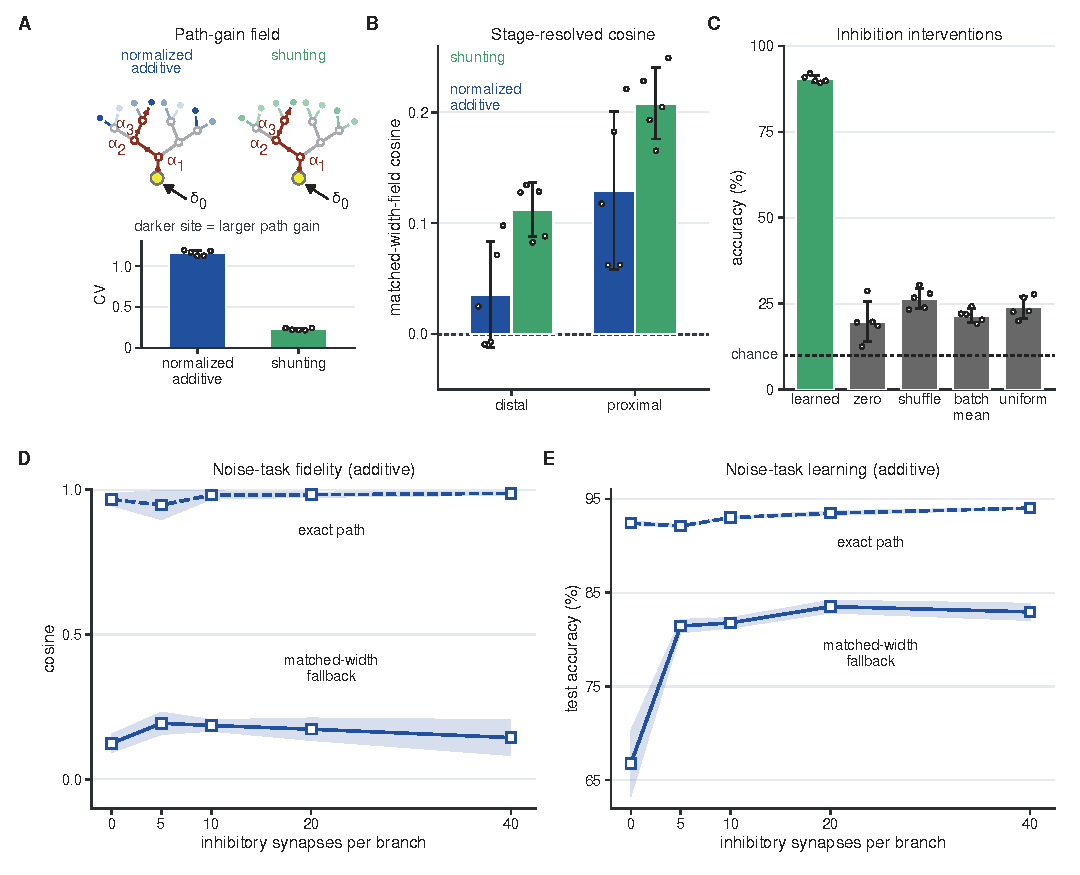
\includegraphics[width=\textwidth]{supplementary/curated/mechanistic_chain.pdf}
\caption{\textbf{Mechanistic chain from path gains to learning in regular-tree models.} MNIST panels \textbf{A--C} use two-stage $[4,4]$ directed trees; the historical noise-resilience panels \textbf{D,E} use two-stage $[3,3]$ additive trees. \textbf{A}, Conductance-stage path-gain field in shunting and normalized-additive models at five inhibitory synapses per branch; the inset shows paired-seed coefficients of variation (CV; standard deviation divided by mean). The schematic is drawn on the shared balanced tree of main Fig.~1B rather than the $[4,4]$ geometry: one root-to-leaf route carries the serial path gains \(\alpha_1\), \(\alpha_2\), \(\alpha_3\), distal sites are tinted by their illustrative path gain (darker, larger) in each model's colour, and \(\delta_0\) is the somatic error. This loading quantity omits branch derivatives and is distinct from the trained exact-error profiles in Supplementary Fig.~S8B,C. \textbf{B}, Stage-resolved cosine of matched-width scalar fallback versus exact MNIST errors; the width-matched somatic stage is excluded because its cosine is one by construction. \textbf{C}, MNIST post-training inhibition interventions: zero, sample shuffle, per-branch batch mean and a uniform matched mean. The dashed rule marks ten-class chance. These also change forward computation and do not isolate backward shunting. \textbf{D,E}, Feedback fidelity and learning on the additive noise task; solid and dashed lines denote matched-width scalar-fallback and exact transport. Bars show standard deviations across checkpoints in \textbf{B} and retained runs in \textbf{C}; shaded bands in \textbf{D,E} show standard deviations across retained runs (0.6--0.9 percentage points at doses 5--40 in \textbf{E}, and below 0.02 for the exact-path series in \textbf{D}, narrower than the marker); white points identify checkpoints in \textbf{B} and runs in \textbf{C}. Historical noise-task shunting aggregates with unresolved execution lineage are excluded and retained in Source Data only. The retained additive aggregates do not resolve their normalization setting. The state-matched focal analysis in main Fig.~8 provides the conductance-specific transport comparison. This chain is the figure support for Supplementary Section~S1; the exact-path field it feeds is drawn at the main-text type scale in main Fig.~1.}
\label{fig:si_mechanistic_chain}
\label{fig:inherited_mechanistic}
\end{figure}

\begin{figure}[p]
\centering
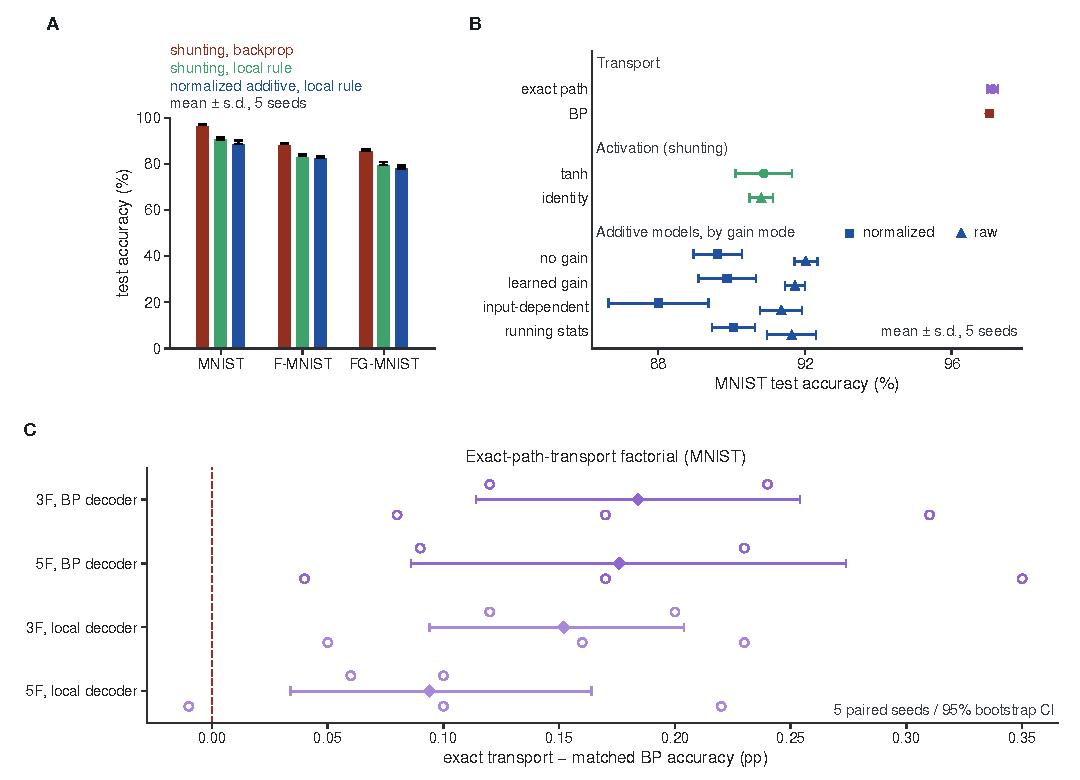
\includegraphics[width=\textwidth]{supplementary/curated/credit_validation.pdf}
\caption{\textbf{Local eligibility and exact transport reproduce the learning gradient.} \textbf{A}, Test accuracy on MNIST, Fashion-MNIST (F-MNIST) and figure-ground MNIST (FG-MNIST) for the shunting architecture trained by backpropagation (red-brown) or by the local rule (green), and for the normalized-additive architecture trained by the local rule (blue); bars are means $\pm$ 1 s.d. across five seeds, and the backpropagation intervals are narrower than the line weight. \textbf{B}, Transport, activation and additive-model implementation controls on MNIST; points are means $\pm$ 1 s.d. across five seeds, and the backpropagation interval is smaller than its marker. Colour names the architecture as in \textbf{A} (red-brown backpropagation, green shunting, blue additive, violet exact path transport); within a family the house marker (circle for shunting, square for additive) is the configuration drawn in \textbf{A} and a triangle is the ablated variant (identity activation without tanh reactivation; raw additive without normalization). The additive group draws the complete normalized/raw $\times$ gain-mode factorial, one gain mode per row. The MNIST backpropagation and normalized-additive conditions in \textbf{A} and \textbf{B} come from different run cohorts (the matched ceiling-refresh and local-rule tuning cohorts in \textbf{A}; the exact-transport and gain-normalization revision cohorts in \textbf{B}): the backpropagation means differ by 0.09 percentage points, and the normalized-additive bar in \textbf{A} lies within the range of the four normalized rows in \textbf{B}. \textbf{C}, Exact-transport-minus-backpropagation accuracy across three-/five-factor and local/backpropagated decoder choices; open circles are five paired seeds, diamonds are condition means and bars are 95\% paired-seed bootstrap intervals; dark violet denotes a backpropagated decoder and lighter violet a local decoder. Exact transport supplies an oracle compartment error. The local three-factor eligibility is sufficient when this error is supplied. Normalized- and raw-additive models are distinct controls; no noise-task shunting aggregate is used here.}
\label{fig:si_credit_validation}
\label{fig:inherited_competence}
\label{fig:inherited_rule_feedback}
\end{figure}

\begin{figure}[p]
\centering
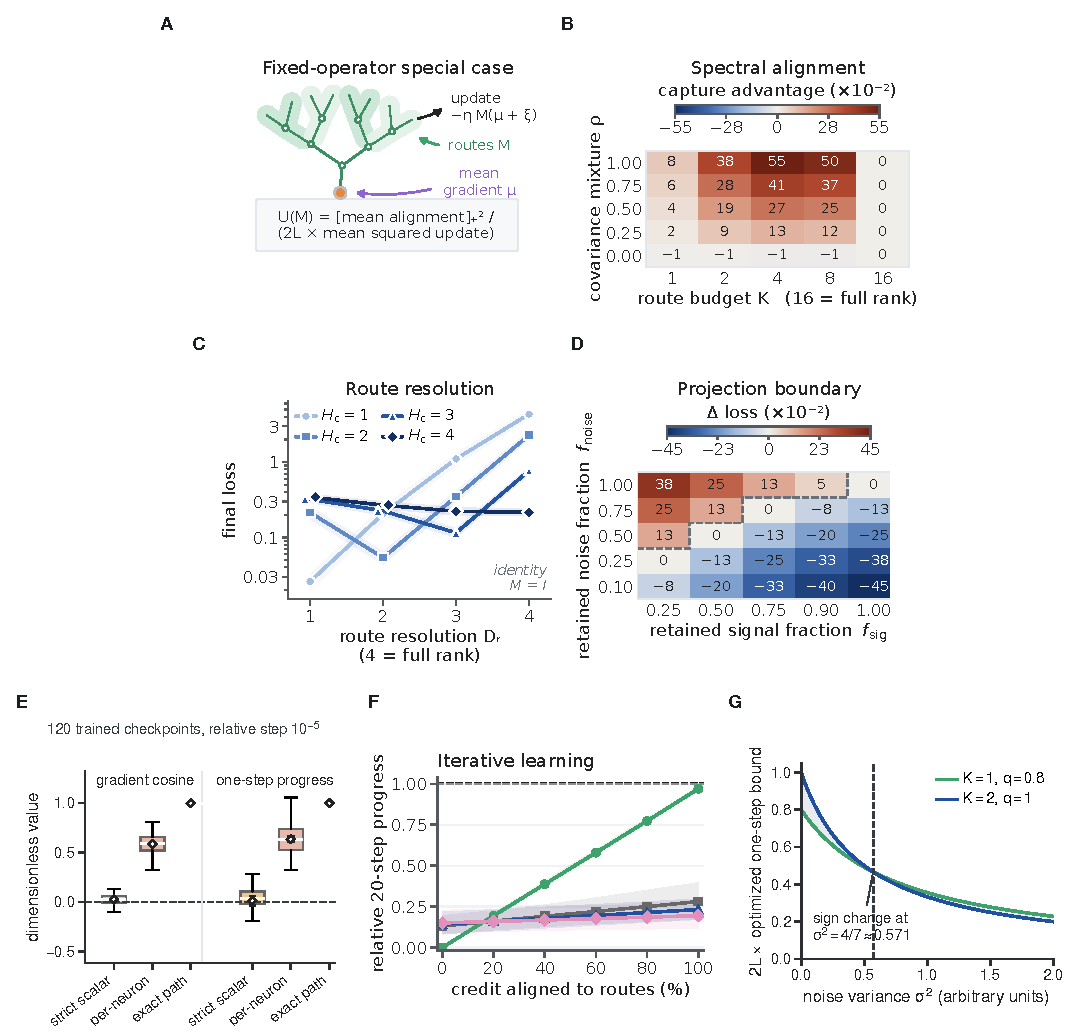
\includegraphics[width=\textwidth]{supplementary/curated/utility_signal_noise.pdf}
\caption{\textbf{Restricted routes trade signal retention against admitted noise, and the one-step quantity is measurable at trained states.} \textbf{A}, Fixed-operator one-step utility bound for the update $M(\bm\mu+\bm\xi)$ (zero-mean noise $\bm\xi$): the boxed $U(M)$, the squared positive part of $\bm\mu^{\top}M\bm\mu$ over $2L\,\mathrm{E}\|M(\bm\mu+\bm\xi)\|^{2}$ ($L$, loss smoothness), lower-bounds the expected one-step loss decrease that \textbf{B--D} sweep. \textbf{B}, Subtree-minus-random spectral capture across route budget $K$ and covariance mixture $\rho$, printed per cell (red positive, blue negative, tint by magnitude); $K=16$ and $\rho=0$ are by-construction controls; only the endpoints are isospectral. \textbf{C}, Final quadratic loss against route resolution $D_{\rm r}$ for hierarchies $H_{\rm c}=1$--$4$, constructed so that fine-scale noise favours an interior resolution; $D_{\rm r}=4$ resolves every leaf ($M=I$); bands, 95\% bootstrap intervals, 50 paired seeds. \textbf{D}, Exact one-step projection boundary: retaining signal fraction $f_{\rm sig}$ and noise fraction $f_{\rm noise}$ changes normalized loss by $(f_{\rm noise}-f_{\rm sig})/2$, printed as in \textbf{B}; unequally spaced fractions form equal cells, so the dashed line is the cell-wise sign boundary, not the diagonal. \textbf{E}, Candidate/exact gradient cosine and norm-matched one-step loss decrease at the same 120 valid trained checkpoints (points; two off-scale strict-scalar values are printed at the floor); exact path is 1 by construction. Boxes, medians, quartiles and 1.5-interquartile-range whiskers; diamonds, means with 95\% checkpoint-bootstrap intervals (one held-out batch, relative step $10^{-5}$) narrower than the marker. \textbf{F}, Separate constructed positive control, eight reconstructed arbors: loss reduction after twenty projected steps versus the full-gradient sequence (green, morphology-selected routes; gray, random paths; blue, depth bins; pink, ancestry-shuffled routes); symbols, cell means with hierarchical 95\% bootstrap intervals. \textbf{G}, Illustrative rank--noise trade-off under isotropic noise, $2L$ times the optimized bound $q^2/(q+K\sigma^2)$ for $(K,q)=(1,0.8)$ (solid) and $(2,1)$ (dashed), crossing at $\sigma^2=4/7$ (shaded between); analytic, no data, not an endpoint-selection prediction. Imposed alignment and oracle projections explain the conditional relationship in \textbf{E,F}, which measures neither biological credit nor a long-horizon selector; the bound is local, and endpoint selection fails prospectively (Fig.~\ref{fig:si_original_selector}).}
\label{fig:si_utility_signal_noise}
\label{fig:supp_alignment}
\label{fig:supp_utility}
\label{fig:si_checkpoint_geometry}
\end{figure}

\begin{figure}[p]
\centering
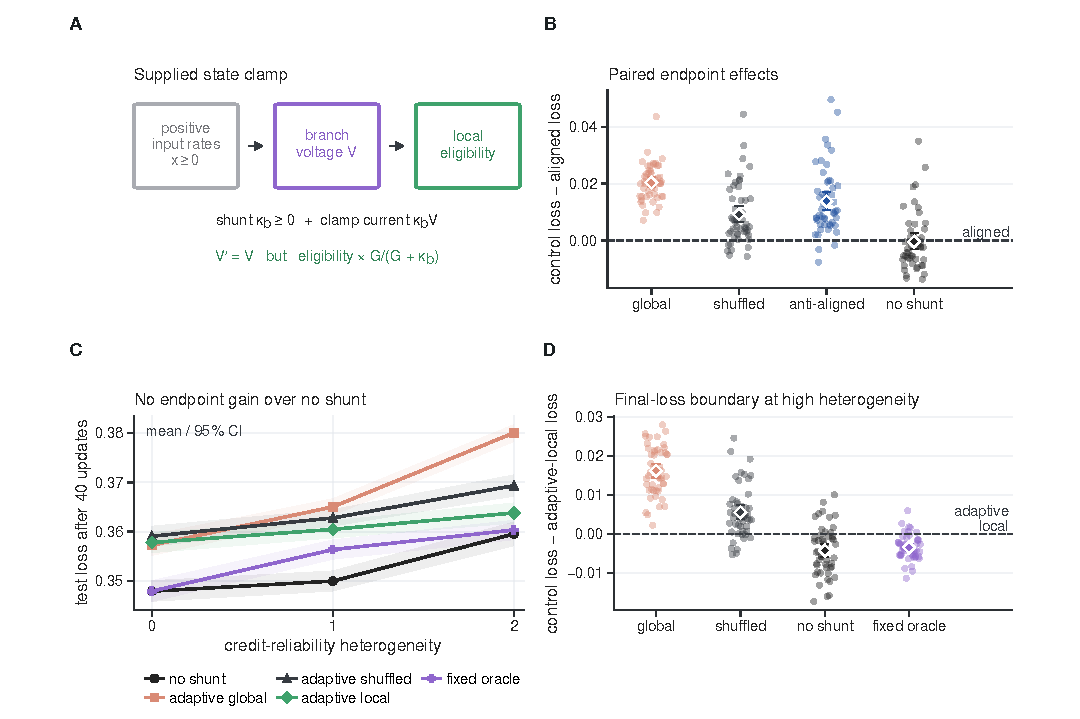
\includegraphics[width=\textwidth]{supplementary/curated/reliability_gain.pdf}
\caption{\textbf{Fixed and estimated reliability gains have bounded learning benefits.} All panels use positive-rate synthetic tasks with eight parallel, nonserial branch blocks. \textbf{A}, A supplied compensating current preserves branch voltage while a positive shunt reduces input resistance and eligibility. \textbf{B}, Paired control-minus-aligned final-loss contrasts at maximal heterogeneity for the best global, shuffled, anti-aligned and unshunted controls; fixed aligned shunting has no reliable final advantage over unshunted noisy learning. \textbf{C,D}, Adaptive-rule final loss and paired control-minus-adaptive contrasts. Adaptive local gain beats global and shuffled attenuation but loses to no shunt and the fixed oracle. In \textbf{B,D} the dashed line is the aligned or adaptive-local reference, translucent dots are the 50 individual paired seeds, and diamonds with bars are means and 95\% paired-seed bootstrap intervals; an interval narrower than its diamond is hidden by it. The point implementation given identical gains reproduces the conductance final loss exactly in all 50 seeds of each study (paired difference 0, 50/50 ties). Curves and shading in \textbf{C} are means and 95\% paired-seed bootstrap intervals across the same 50 seeds. The supplied compensating current in \textbf{A} and the paired gradient observations from which the adaptive rule in \textbf{C,D} estimates its gains are explicit information resources.}
\label{fig:si_reliability_gain}
\label{fig:supp_positive_reliability}
\label{fig:supp_adaptive_reliability}
\end{figure}

\begin{figure}[p]
\centering
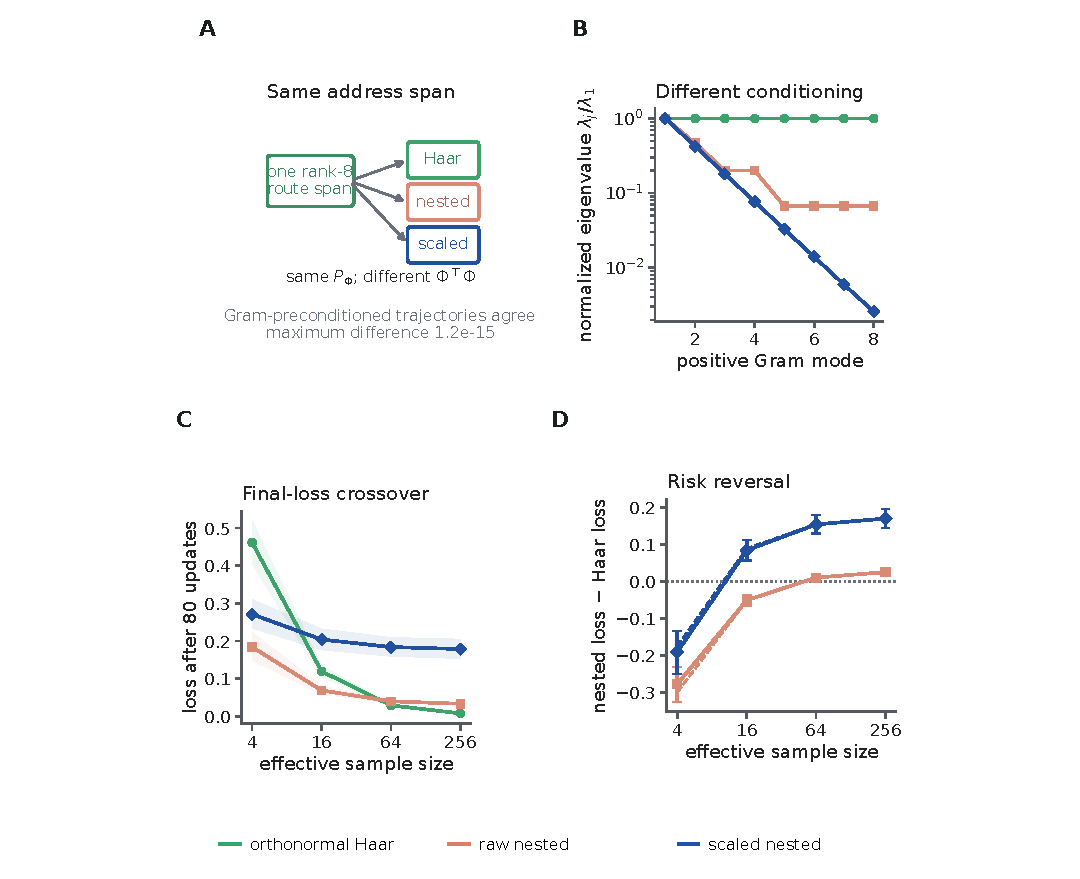
\includegraphics[width=\textwidth]{supplementary/curated/same_span_conditioning.pdf}
\caption{\textbf{Identical route spans can learn differently through conditioning.} \textbf{A}, Haar, raw nested (redundant) and scaled nested (statically scaled) coordinates parameterize the same rank-eight span in sixteen abstract coefficients. \textbf{B}, Positive Gram eigenvalues; condition numbers are 1, 15 and 388.52. \textbf{C}, Population loss after eighty updates across effective sample size on a logarithmic axis; curves and bands are means and 95\% seed-bootstrap intervals across fifty seeds. The strip above the axis shows, for every seed, the predicted effective sample size at which the exact finite-time risks of the nested and Haar coordinates are equal (raw nested: median 38.5, interquartile range 31.1--63.7; scaled nested: median 8.2, interquartile range 6.3--12.6); large symbols and dotted guides mark the medians. \textbf{D}, Paired nested-minus-Haar contrasts; negative values favor nested coordinates. Points and bars are means and 95\% paired-seed bootstrap intervals across fifty seeds (n = 50 pairs); dashed curves are the exact finite-time risk. Slow modes reduce variance at low data and retain bias at high data. Gram-preconditioned controls agree to $1.15\times10^{-15}$. This is a coefficient-learning comparison within one span, not a simulation of forward dendritic morphology or a biological implementation of the preconditioner.}
\label{fig:si_same_span_conditioning}
\label{fig:supp_same_span_learning}
\end{figure}

\clearpage

% Curated from paper commit 7ee9157; generators and exclusions retained.
\section{Image benchmarks and feedback controls}
\label{note:credit_images}
\label{note:artificial}

\subsection{Shared architecture, data and local optimization}

The MNIST core contains one dendritic population of 128 neurons, with no separate inhibitory-cell population. Each neuron has a soma, three proximal compartments and nine distal compartments, denoted $[3,3]$. Separate TopK arrays select 40 excitatory and 20 inhibitory contacts from the 784 pixels at each nonsomatic compartment. There are no somatic input synapses: 92,160 active contacts are selected from 2,408,448 candidate synaptic parameters. Inactive local weights are not updated. Softplus transforms enforce nonnegative synaptic and coupling parameters. A linear $128\times10$ decoder gives ten class scores. The complete network has 2,414,602 parameter slots, including 1,290 decoder parameters.

Pixels are divided by 255 and flattened without additional normalization or augmentation. Each seed divides the 60,000 official training images into 48,000 fitting and 12,000 validation examples; the official 10,000-image test set is held out. The shared MNIST recipe uses three-factor local eligibility, batches of 256, 180 epochs and Adam with $(\beta_1,\beta_2,\epsilon)=(0.9,0.999,10^{-8})$, without weight decay or mixed precision. After minibatch averaging, input, coupling, reactivation and decoder gradients are clipped elementwise to $[-5,5]$. Their original learning rates are $1.5\times10^{-3}$, $7\times10^{-4}$, $5\times10^{-4}$ and $1.5\times10^{-3}$, respectively. Early stopping is disabled and minimum validation loss selects the retained checkpoint. Deterministic PyTorch settings disable TF32 and cuDNN benchmarking and use the highest float32 matrix-multiplication precision.

Every compartment uses the learned output nonlinearity
\begin{equation}
f_n(V)=\frac{\tanh[m_n(V-b_n)]+1}{2},\qquad
f_n'(V)=\frac{m_n}{2}\{1-\tanh^2[m_n(V-b_n)]\},
\label{eq:s_parametric_tanh}
\end{equation}
where $m_n$ and $b_n$ are slope and midpoint. Shunting trees use analytical initialization. Raw-additive trees use the prespecified occupancy-quantile policy: empirical voltage quantiles 0.1 and 0.9 map to outputs 0.1 and 0.9, with minimum quantile width $10^{-3}$, maximum slope 50 and reversion on an invalid fit. The comparisons therefore retain the architecture-specific initialization policies, not identical initial voltage scales.

\subsection{Additive controls and gradient coordinates}

The raw-additive alias \texttt{dendritic\_additive} disables both shunting and additive normalization. Its current sums and local derivatives are
\begin{align}
J_n^{\mathrm E,\mathrm{add}}&=\sum_{i\in\mathcal S_n^{\mathrm E}}g_i^{\mathrm E}x_i^{\mathrm E},&
J_n^{\mathrm I,\mathrm{add}}&=\sum_{j\in\mathcal S_n^{\mathrm I}}g_j^{\mathrm I}x_j^{\mathrm I},\\
J_n^{\mathrm{child},\mathrm{add}}&=\sum_{c\in\mathcal C_n}g_{c\to n}^{\mathrm{den}}a_c,&
V_n^{\mathrm{add}}&=J_n^{\mathrm E,\mathrm{add}}-J_n^{\mathrm I,\mathrm{add}}+J_n^{\mathrm{child},\mathrm{add}},
\label{eq:s_additive_forward}
\end{align}
with $a_n=f_n(V_n^{\mathrm{add}})$, and
\begin{equation}
\frac{\partial V_n^{\mathrm{add}}}{\partial g_i^{\mathrm E}}=x_i^{\mathrm E},\quad
\frac{\partial V_n^{\mathrm{add}}}{\partial g_j^{\mathrm I}}=-x_j^{\mathrm I},\quad
\frac{\partial V_n^{\mathrm{add}}}{\partial g_{c\to n}^{\mathrm{den}}}=a_c,\quad
\delta_c^V=\delta_n^Vg_{c\to n}^{\mathrm{den}}f_c'(V_c).
\label{eq:s_additive_derivatives}
\end{equation}
Inhibition contributes a subtractive current, not a negative conductance. Raw-parameter gradients include the softplus derivative. The inherited normalized-additive control instead standardizes each example across a stage's output coordinates. With $Z_{sn}=J_{sn}^{\mathrm E,\mathrm{add}}-J_{sn}^{\mathrm I,\mathrm{add}}+J_{sn}^{\mathrm{child},\mathrm{add}}$, it uses
\begin{equation}
V_{sn}^{\mathrm{norm}}=\frac{Z_{sn}-\langle Z_{s\cdot}\rangle_n}{\operatorname{sd}_n(Z_{s\cdot})+\epsilon},
\qquad a_{sn}=\frac{\tanh(0.1V_{sn}^{\mathrm{norm}})+1}{2}.
\label{eq:s_historical_normalized_additive}
\end{equation}
Its fixed slope and midpoint are 0.1 and zero. Because this changes forward computation, its outcomes are not pooled with raw-additive results.

The fresh dictionary experiment routes errors of compartment output activation; $f'_n$ remains in local eligibility, including gate-parameter derivatives. Neuron-specific feedback repeats each exact somatic error within that tree. The projected $K=1$ rule averages exact activation errors over all twelve nonsomatic compartments; $K=3$ averages them separately within each proximal compartment and its three children. Both acquire coefficients from the same exact field and preserve its common mean at identical weights, but need not preserve equal field norms. Their somatic error remains exact. Strict scalar instead reduces the neuronal error vector at every core stage, including the soma, using Eq.~\ref{eq:s_scalar_reduction}. Exact transport retains every compartment error. The linear decoder receives exact gradients in all arms. Decoder-only learning suppresses core and gate gradient writeback; initial/final core hashes verify the intended freeze. These projected comparisons test delivery capacity with oracle coefficients.

\subsection{Fresh dictionary controls and retained image cohorts}

The six-rule MNIST experiment compares common rate multipliers $0.3,1,3$. Three development seeds per architecture, rule and multiplier give 108 fits. A separately frozen addendum specified projected $K=1$ before fresh outcomes, with the same tuning procedure. Mean minimum validation loss selects each rule's multiplier. Ten new paired seeds per architecture and rule then test the selected rate and, when different, the original multiplier one. Coincident conditions reuse a fit, giving 190 unique fresh fits; twelve three-epoch canaries are excluded. Pairing covers initialization, contacts, splits and minibatches. Descriptive intervals use 50,000 whole-seed bootstrap draws. Full configurations and seed endpoints are in \texttt{source\_data/image\_ladder\_controls/}.

Capture was measured at initial and exact-trained checkpoints on the first 2,048 official test images. For each example/neuron, the field comprises twelve nonsomatic errors. The primary endpoint averages nonzero field-wise squared-energy ratios; aggregate energy capture is also retained. Activation-space capture matches the trained projections, while voltage-space capture preserves the earlier diagnostic coordinate. Two historical checkpoints reproduced their recorded voltage captures to numerical precision; instrumentation left outputs unchanged. In the earlier fifteen-seed cohort, moving from one to three profiles increased mean voltage-credit capture from 0.480 to 0.625 in shunting trees and from 0.519 to 0.718 in additive trees. These values describe a separate cohort and coordinate from the activation-error capture in main Fig.~1G.

The original MNIST ladder uses seeds 42--56: strict scalar, neuron-specific and exact credit in both architectures give 90 fits; matched-width scalar fallback adds 30. The latter differs from strict scalar in a small near-somatic parameter group, as quantified in Section~\ref{note:rules}. These consistently executed runs replace the superseded mixed-source set; the replacement decision preceded outcome inspection. The independent direct-feedback-alignment factorial uses fifteen paired seeds per dynamics and 120 new fits with frozen exact-readout references. A seed-fixed Gaussian output-to-neuron matrix, scaled by inverse square root of output dimension, replaces the decoder derivative. Ownership controls permute neuronal recipients without changing values or bandwidth.

Fashion-MNIST retains the MNIST architecture, contacts, optimizer, initialization and 180-epoch budget without retuning. Seeds 10200--10209 pair 48,000/12,000 fitting/validation images and the 10,000-image official test set. Sixty fits cross two architectures with matched-width scalar fallback, neuron-specific and exact fields. Neuron-specific-minus-fallback accuracy is 4.46 percentage points (95\% interval 4.09--4.88) for shunting and 3.78 (3.43--4.14) for additive trees; all ten differences are positive in each. Exact-minus-neuron-specific differences are $-0.11$ ($-0.21$ to $-0.01$; 2/10 positive) and 0.13 ($-0.08$ to 0.35; 8/10). The prespecified neuronal-identity criterion required at least 8/10 positive differences and an interval above zero in each architecture. All sixty fits were complete and finite without feedback fallbacks. Full means and tests remain in \texttt{source\_data/fashion\_feedback\_ladder/}.

\subsection{CIFAR-10 and exact-gradient validation}

The raw-additive CIFAR-10 cohort uses flattened images, no augmentation or normalization, a 90:10 training/validation split, one 20-soma $[3,3,3,3]$ population, 25 contacts of each sign per branch and a 20--32--16--10 decoder. The realized \texttt{input\_mode=1} model has direct excitatory/inhibitory inputs and no inhibitory-cell population. A validation-only BP screen jointly selected adaptive initialization and empirical stage calibration from three batches; it cannot attribute their benefit separately. A provisional configuration with mean BP accuracy 38.98\% was excluded for an inadequate operating point. The selected three-seed calibration reached 49.960\% validation and 49.723\% test accuracy. A separate five-seed check reproduced normalized-additive and shunting reference endpoints to within 0.026 percentage points.

All four fresh rules use Adam at $10^{-3}$, batch size 256, at most 200 epochs, patience 40 and the validation-best checkpoint. Weight decay is zero; the separate 0.01 configuration field controls sparse-weight maintenance. Seeds 10800--10819 give eighty finite, complete fits. Mean accuracies are 0.34472 (strict scalar), 0.50865 (neuron-specific), 0.50006 (exact path) and 0.50122 (matched BP). The exact-minus-neuron-specific difference is $-0.00859$ (95\% interval $-0.01171$ to $-0.00547$; 2/20 positive), so the exact-path superiority criteria fail. Exact-minus-BP is $-0.00115$ ($-0.00457$ to 0.00226), with two one-sided tests supporting equivalence within $\pm0.01$ (90\% interval $-0.00398$ to 0.00167; $P=1.58\times10^{-5}$). This is a compact transfer assay, not a competitive vision benchmark.

A separate five-seed exact-transport factorial (42--46) crosses three-/five-factor rules with local/BP decoder updates over 200 epochs and a ReLU core output. Local rates for input, coupling, reactivation and decoder are $1.5\times10^{-3},7\times10^{-4},5\times10^{-4},1.5\times10^{-3}$; matched BP uses $10^{-3},5\times10^{-4},5\times10^{-4},10^{-3}$. Analytic and automatic gradients were compared in 100 diagnostic runs: median relative error $7.43\times10^{-8}$, maximum $1.88\times10^{-7}$, with parameter tensors as diagnostic units. The architectures and method-specific rates above distinguish these protocols.

\subsection{Depth, ownership and input-map controls}

The original depth-by-feedback factorial crosses two tasks, two cores, stages D1--D4, three local fields plus BP and ten seeds: 640 planned fits. Completeness requires the specified seed/configuration, checkpoint and full curves, expected stages, nondegenerate couplings, finite metrics and no transport-shape fallback. All completed, but a later outcome-independent validity check excludes 160 synthetic-noise shunting fits with signed conductance drive. The retained 480 fits contain both cores on MNIST and additive noise-task models. Depth changes compartment and parameter count. The ownership comparison at D2/D4 retains 120/160 fits after the same exclusion. A 400-fit inhibitory-dose family is entirely excluded from inference because its primary shunting contrast uses invalid signed input, although configurations and exclusion records remain available.

The clean exact/BP rerun instead uses valid inputs: two tasks, two cores, four depths, two methods and seeds 42--51 give 320 fits. Shunting uses explicit ReLU transfer; additive noise inputs remain signed. Source commits are \texttt{74792ca9} for implementation and \texttt{4f3612a5} for the nested generator. All 320 fits are finite and complete; 42 use streaming evaluation of a terminal metric. Failed attempts with missing generator code, insufficient memory or rejected signed shunting have no included endpoint. Re-executed configurations retain their scientific settings. Comparisons first average four depths within each seed, then use 20,000 paired bootstrap draws and descriptive Wilcoxon tests. Across all 160 method pairs, mean exact-minus-BP accuracy is $-0.0545$ points; the largest absolute pair difference is 5.90 points. This does not establish pointwise equality.

The spatial-input control uses depth four, 21 contacts per distal branch and 320 planned fits. Spatial branches recursively partition the $28\times28$ feature plane into sixteen disjoint regions; random branches sample all 784 coordinates. The 240 conductance-valid fits cross maps, methods, cores and tasks; the noise task retains only additive models. Persistence under BP and random task projection identifies a forward input-coverage effect. A separate 320-fit noise comparison holds sixteen terminal branches and 960, 960, 968 or 960 active contacts per soma across D1--D4; it retains 160 additive fits. Compartments, couplings and reactivation parameters still increase with depth.

At 120 valid BP checkpoints, a fixed held-out batch compares scalar fallback, neuron-specific and exact fields using nonsomatic stages and trainable branch parameters only. Outcomes are optimally scaled field capture, eligibility-weighted gradient capture/cosine and norm-matched loss change. Relative step $10^{-5}$ is primary; $10^{-6},10^{-4},10^{-3}$ are sensitivity values. Checkpoints are neither updated nor selected by this diagnostic, and bootstrap resampling preserves paired fields. Complete controls and validity accounting accompany the figure-linked Source Data (Supplementary Fig.~\ref{fig:si_checkpoint_geometry}).

\subsection{Identity of the historical noise tasks}

The key \texttt{noise\_resilience} named two generators. The clean rerun's recovered source, commit \texttt{4f3612a5}, draws class $y$ uniformly from $\{0,1,2\}$ and constructs a square image $L_y$: blank, a uniformly selected horizontal row of ones, or a uniformly selected vertical column of ones. It returns
\begin{equation}
x=\operatorname{vec}(L_y+0.2\varepsilon),\qquad
\varepsilon_{ab}\overset{\mathrm{iid}}{\sim}\mathcal N(0,1).
\label{eq:legacy_noisy_lines}
\end{equation}
The executed dispatcher's default side length is 784, giving 614,656 inputs, independently confirmed by checkpoint sizes. Its 10,000 unnormalized, unclipped examples split into 8,000/1,000/1,000 fitting/validation/test samples using run-seeded generators. Projected-noise fields in launch configurations were ignored. Thus these rows test implementation agreement on three classes, not corrupted-MNIST robustness.

The documented prospective depth/routing/dose/fixed-budget protocol instead perturbs MNIST digits as
\begin{equation}
\widetilde x=\operatorname{clip}_{[0,1]}(x+1.5Pz),\qquad z\sim\mathcal N(0,I_{50}),
\label{eq:projected_noise_mnist}
\end{equation}
where $x\in[0,1]^{784}$, $P\in\mathbb R^{784\times50}$ has independent normal entries and unit-norm columns, and digit labels are unchanged. Projection seed is zero; training/validation/test latent-noise seeds are 1/2/3. The intended splits are 48,000/12,000/10,000 without further gain or normalization. Frozen configurations and model sizes support this intended protocol, but no hash of the executed nested generator survives. The fixed-budget outcome/validity join also lacks raw resolved configurations and does not close that gap.

Inherited aggregate feedback/gradient panels lack a complete run-to-generator join. Twenty-six historical shunting points remain unresolved and are excluded from conductance-valid figures and inference; neither generator is assigned to them retrospectively. The fixed-budget audit retains 160 additive and excludes 160 signed-shunting outcomes. The release exposes \texttt{legacy\_noisy\_lines} and \texttt{projected\_noise\_mnist} separately and rejects the ambiguous key without explicit choice. The latter is a frozen implementation of the documented protocol, not recovered historical execution. See \texttt{source\_data/release\_task\_identity/task\_identity.json} and \texttt{source\_data/review\_curve\_lineage/}.

Inherited regime sweeps use five seeds per condition; Gaussian broadcast noise is scaled relative to the original teaching signal, and depth varies at fixed somatic width. Their normalized-additive, raw-additive and shunting variants remain separate. They test operating regimes, not isolated backward effects of inhibition.

\begin{figure}[p]
\centering
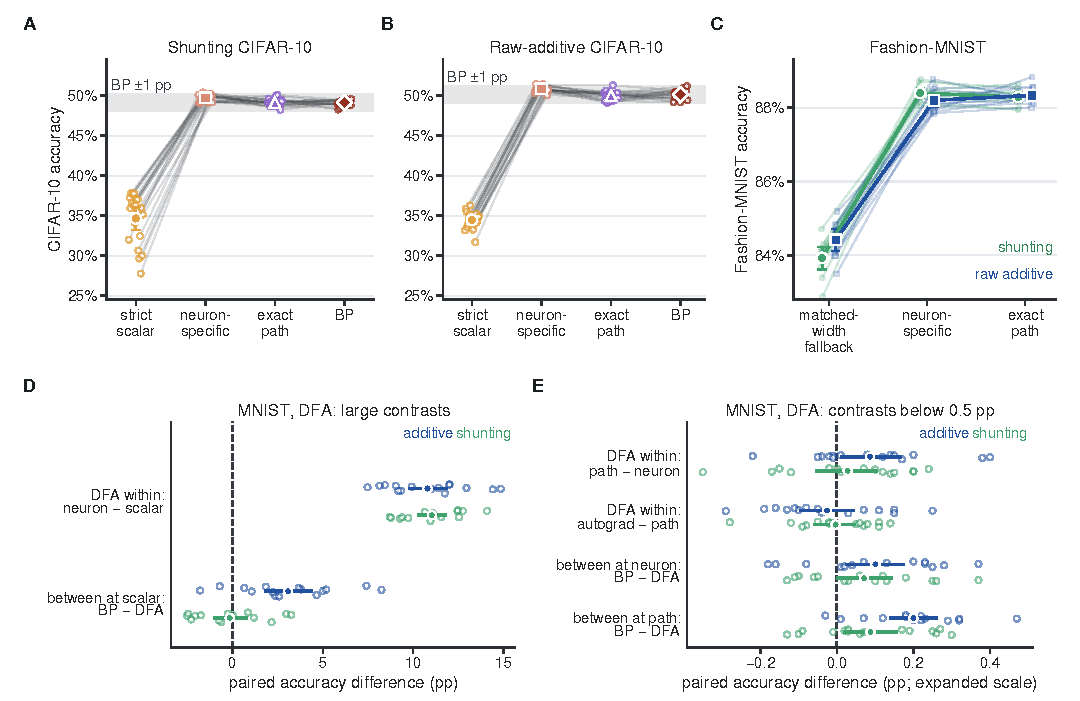
\includegraphics[width=\textwidth]{supplementary/curated/image_generalization.pdf}
\caption{\textbf{The neuron-identity bottleneck generalizes across image and feedback controls.} \textbf{A}, Flattened CIFAR-10 in the shunting architecture, with matched-width scalar fallback, random rank-four, exact-path and backpropagation rules (five seeds). \textbf{B}, Raw-additive CIFAR-10 with strict scalar, neuron-specific, exact-path and backpropagation feedback (twenty paired seeds; 95\% Student-$t$ intervals). Exact path is 0.859 percentage points below neuron-specific feedback and equivalent to backpropagation within the prespecified one-point margin. \textbf{C}, Fashion-MNIST in shunting and raw-additive trees (ten paired seeds; 95\% bootstrap intervals); path resolution adds no reliable benefit. \textbf{D,E}, Dominant and sub-point contrasts under fixed random soma feedback (DFA), with fifteen paired MNIST seeds and 95\% bootstrap intervals. DFA preserves the neuron-versus-scalar benefit, but does not add a second dendritic layer or increase the dimensionality of the ten-class readout error. Percentage-point scales differ.}
\label{fig:si_image_generalization}
\label{fig:regular_regimes}
\label{fig:supp_between_within_factorial}
\end{figure}

\begin{figure}[p]
\centering
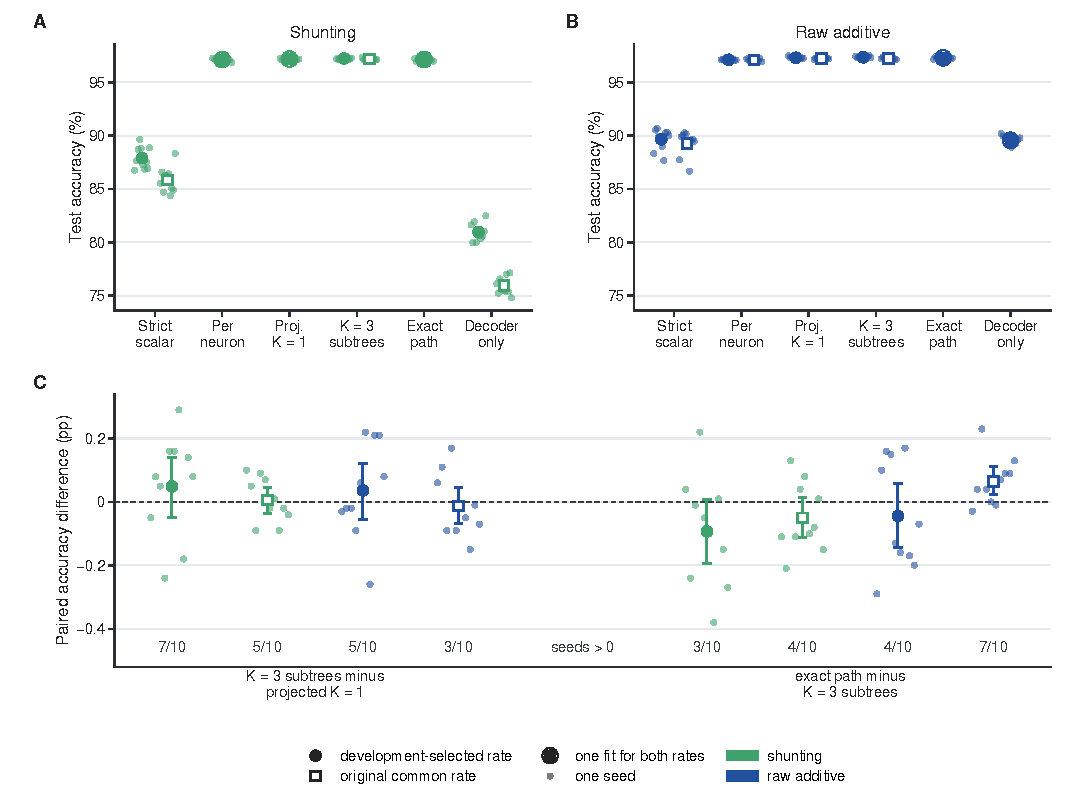
\includegraphics[width=\textwidth]{supplementary/curated/mnist_dictionary_geometry.pdf}
\caption{\textbf{Intermediate dictionaries capture more image-task credit without improving accuracy.} \textbf{A,B}, Six-rule MNIST ladder in shunting and raw-additive networks; ten fresh paired seeds per architecture. Filled/open symbols use development-selected/original common rates. Decoder-only learning freezes the initialized core. \textbf{C}, Paired accuracy differences for three profiles versus a projected common profile, and exact versus three-profile credit. \textbf{D}, Initial and trained activation-error capture by one or three profiles, averaged over 2,048 images within each seed. Projection coefficients use the exact field. Means and bars in A--D have descriptive 95\% seed-bootstrap intervals. \textbf{E--G}, Independent fifteen-seed cohort: common-state branch-gradient cosine, soma-normalized exact voltage-error magnitude by depth, and within-depth path-specific error energy. These distinguish direction, amplitude and spatial variation; exact-path cosine one is definitional. Greater path-specific variation did not yield an image accuracy benefit. Voltage- and activation-space capture are different quantities. All image cohorts have one dendritic layer and a linear readout.}
\label{fig:si_mnist_dictionary_geometry}
\label{fig:supp_image_diagnostics}
\label{fig:supp-image-ladder-controls}
\end{figure}

\begin{figure}[p]
\centering
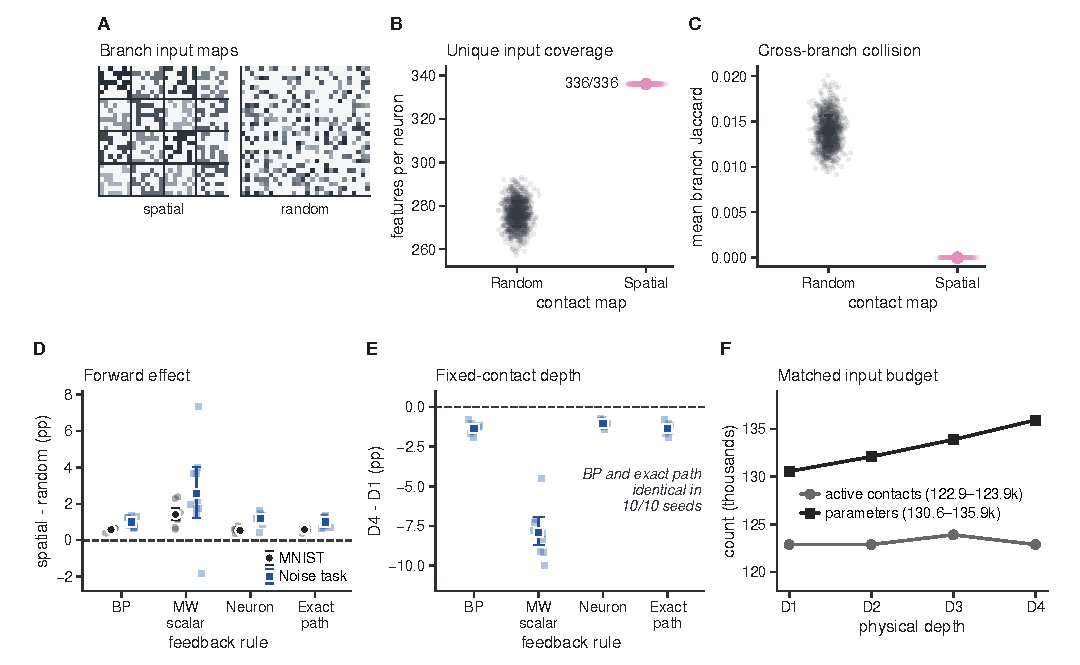
\includegraphics[width=\textwidth]{supplementary/curated/input_coverage_depth.pdf}
\caption{\textbf{Input coverage and ordinary-task depth are distinct from credit resolution.} \textbf{A--D}, Spatial versus randomly assigned contacts in depth-four $[2,2,2,2]$ trees: example map, unique input coverage, cross-branch overlap and learning benefit under backpropagation and three local fields. Contact count is matched, but spatial maps reach more unique inputs and avoid collisions. The accuracy benefit persists under backpropagation and therefore reflects a forward sparsity prior. \textbf{E,F}, Separate raw-additive historical noise cohort with sixteen terminals: all four D4-minus-D1 accuracy contrasts are negative in 10/10 paired seeds; active contact counts are approximately fixed while parameter counts vary. Learning contrasts use means and 95\% paired-seed bootstrap intervals; map summaries use mean $\pm$ s.d. The noise-task executed generator remains unresolved and its shunting runs fail the positive-conductance input criterion. These retained additive outcomes are a depth boundary, not evidence for shunting; exclusions are enumerated in Table~\ref{tab:input_validity}.}
\label{fig:si_input_coverage_depth}
\label{fig:supp_spatial_audit}
\label{fig:supp_fixed_budget}
\end{figure}

\clearpage

% Curated from paper commit 7ee9157; original equations and protocol identities retained.
\section{Branch conflict, ancestry routing and coefficient learning}
\label{note:conflict_ancestry}

\subsection{Context-gated Fashion-MNIST protocol}

The context-gated task used Fashion-MNIST classes 0 and 6. Inputs were
average-pooled to $7\times7$, standardized using training data and augmented
with a constant coordinate. Each seed used
8,192 training and 2,000 test draws with replacement from the official binary
splits, balanced across context and label. Branch counts were $B=2,4,8$;
conflict doses were $0,0.25,0.5,4/7,0.6,2/3,0.75,1$. Thresholding one
underlying uniform mask made conflict nested across doses. Correct, shared,
cyclically deranged, BP and gated-point rules reused inputs and initialization.
Full-batch descent used 250 updates at step 0.04 and an initial weight
standard deviation (SD) of 0.01.
Three exploratory seeds (100--102) selected a stable setting; an additional
implementation-check seed was also excluded. Analysis seeds 11000--11019
were fixed before outcomes, with no outcome-dependent stopping.

The primary estimand was each seed's least-squares slope of
correct-minus-shared accuracy on conflict, separately for each $B$.
Prespecified criteria required positive slopes in at least 16/20 seeds,
at least ten percentage points of separation at full conflict, less than
two points at zero conflict, correct routing above derangement and exact
BP/gated-point agreement. All criteria passed. The maximum analytic-versus-
autodifferentiation discrepancy was $3.43\times10^{-7}$; equivalent-rule
accuracy differences were zero. Intervals used 20,000 paired-seed bootstrap
draws; tests were two-sided Wilcoxon tests. Mean-field assumptions and empirical
chance crossings are distinguished below.

The same twenty seeds were replayed for post hoc gradient diagnostics at epochs 0, 1, 10, 50, 100 and 250, comparing both each method's own state and a common exact-rule state. Official input-file checksums were verified; the input manifest and all 28,800 rows are retained in \texttt{source\_data/review\_branch\_trajectories/}. Endpoint drift was below $5\times10^{-9}$ in loss. At conflict 0.5, common-state shared-gradient cosine fell from 0.987 to $-0.519$ for four branches and from 0.952 to $-0.701$ for eight branches by epoch 250 (Supplementary Fig.~\ref{fig:si_branch_conflict_controls}). The initialization boundary below was retained without refitting; trained gradient direction and trained accuracy crossing are separate endpoints.

\subsection{Mean-field boundary for context-gated branch selection}

The Fashion-MNIST conflict experiment selects one branch $c$ uniformly from
$B$ branches. Only $\bm w_c^{\mathsf T}\bm x_c$ enters the logit, so the
exact derivative of every unselected branch is zero. Shared feedback omits
that selector and updates every active eligibility. For the centered
mean-field prediction, assume balanced class signs $s\in\{-1,1\}$,
class means $\E[\bm x\mid s]=s\bm v$, and zero logits, so the logistic
error is $\delta=-s/2$. An unselected input copies the selected image with
probability $1-\chi$ and is independently drawn from the opposite class
with probability $\chi$. Its mean class evidence relative to the selected
view is therefore $1-2\chi$. The resulting compatibility matrix is
\[
C_\chi=(1-2\chi)\bm 1\bm 1^{\mathsf T}+2\chi I.
\]
Its shared-mode eigenvalue is $B-2\chi(B-1)$, which vanishes at
$\chi_c=B/[2(B-1)]$. Under these population and initialization assumptions,
the expected shared update loses positive alignment with the exact update
at that boundary. Logistic derivatives and class-conditional moments need
not preserve this relation as weights change. The empirical trained
chance crossing is consequently a separate descriptive endpoint, not a
theorem about the entire optimization trajectory. The missing branch
selector may be supplied in feedback or in local eligibility; it is not
evidence that the unselected branches require opposite exact errors.

\subsection{Two-branch subtree-address experiment}

The minimal two-sibling experiment used ten paired seeds (4100--4109), following an excluded numerical-check seed 4099. The check verified nondegenerate shared capture, exact-route capture one and analytic exact/BP agreement. The subsequent eight-stream factorial varied route budget.

For seed-specific unit vectors $\bm u_A$ and $\bm u_B$, binary label sign
$y\in\{-1,1\}$ and context $c\in\{0,1\}$, the two input means were
\begin{align}
\mathbb E[\bm x_A\mid y,c]
&=y\,[\mathbb 1(c=0)-0.75\mathbb 1(c=1)]\bm u_A,\\
\mathbb E[\bm x_B\mid y,c]
&=y\,[\mathbb 1(c=1)-0.75\mathbb 1(c=0)]\bm u_B.
\label{eq:s_credit_reversal_task}
\end{align}
Each stream had 12 coordinates and independent Gaussian noise with standard
deviation 1.15. The 2,048-example train and test splits contained exactly 512
examples in each context--label cell. The somatic logit selected branch $A$
when $c=0$ and branch $B$ when $c=1$. Both inputs nevertheless remained
active, preventing the one-coordinate rule from acquiring branch specificity
through a zero eligibility on the distractor.

For somatic logit $z$ and logistic sigmoid $\sigma$, let
$\delta=\sigma(z)-\mathbb 1(y=1)$ and
$\bm r(c)=(\mathbb 1[c=0],\mathbb 1[c=1])$. Exact and correct-subtree
coefficients were $\delta\bm r(c)$; within-neuron derangement reversed the
two entries, giving $\delta\bm r(c)_{::-1}$; the shared neuronal and same-depth controls used
$\delta(1,1)$; and the random rank-two control used
$\delta\bm r(c)R_s^{\mathsf T}$ for a seed-fixed orthogonal rotation $R_s$.
The gated point emulation used one somatic coefficient together with the
context-gated features $(\mathbb 1[c=0]\bm x_A,
\mathbb 1[c=1]\bm x_B)$, making its alternative address resource explicit.
All conditions had 24 trainable weights and the same paired initialization and
batch order. The random dense control had four routing nonzeros; the sparse
two-route conditions had two.

Training used mini-batch stochastic gradient descent (SGD), learning rate 0.3,
batch size 64 and 60 epochs.
The switch endpoint applied another 12 epochs to 1,024 context-1 examples with
balanced labels and measured the change in context-0 accuracy. For gradient
geometry, exact and candidate per-example gradients were concatenated over
both branches. Scaled capture was squared cosine after optimal scalar
rescaling. The one-step candidate was normalized to the exact batch-gradient
norm and evaluated at step 0.25. The Source Data indexed in Table~\ref{tab:source_index} retain every
tested condition; no condition was removed on the basis of its outcome.

All controls, including poor deranged and variable random-map outcomes, are retained. Correct routing, exact transport, BP and gated-point emulation coincide because the exact path coefficient is the binary selector. Thus this experiment isolates the supplied address resource; the gated-point control reproduces it.

\subsection{Subtree-address bandwidth and architecture factorial}

To vary feedback bandwidth, the complete factorial extended the two-sibling
task to eight context-selected streams arranged in a balanced binary hierarchy. Context and binary
label were exactly balanced in train and test sets, every stream remained
active on every example, and the sign of the task signal reversed outside the
selected context. Thus a shared coefficient could not recover the required address simply
because off-route eligibilities were zero. The prespecified feedback budgets
were $K\in\{1,2,4,8\}$ nested routes. Twenty paired analysis seeds
(4200--4219) crossed five representations and 27 method--budget combinations,
giving 135 fits per seed and 2,700 fits in total.

The dendritic tree, explicitly gated point model, flat-compartment model and
grouped-point model were implementation-equivalent controls: each contained 64
trainable weights, 64 active input contacts and one output nonlinearity, and
each received the same routed coefficient field. The fifth representation was
a degree- and depth-matched rewired tree. Its resource counts were unchanged,
but its ancestry groups were permuted relative to the task hierarchy. Feedback
families comprised correct ancestry, fixed within-neuron derangement,
depth-interleaved groups, random sparse groups, a seed-fixed random rank-$K$
map, and a task-fitted rank-$K$ upper bound. Neuron-shared, exact-transport and
analytic-backpropagation references completed the design. Route fields were
unit-normalized per example. Data, initialization and every
stochastic control map were keyed to seed, method family and $K$, so matched
representations saw identical stochastic realizations.

Pre-analysis checks required balanced labels and contexts, nonzero activity in every stream, shared capture below 0.2, exact capture one, analytic exact/BP equality and no fallback. An initial 2,700-fit cohort used stochastic maps unpaired across representation labels and was excluded. Only the complete repeat with paired maps and cross-representation equivalence checks enters inference.

The primary bandwidth contrasts are retained in the Source Data indexed in Table~\ref{tab:source_index}.
Correct nested-subtree routing strongly exceeded route derangement at $K=2$ and $K=4$, but
its comparison with the best matched non-anatomical control was deliberately
more stringent: ancestry lost at $K=1$ and $K=2$, won by 0.0127 accuracy at
$K=4$ (95\% paired seed-bootstrap interval 0.00593--0.01946; 15/20 seeds;
paired Wilcoxon signed-rank Holm-adjusted $P=0.0101$ across the four budgets;
the Source Data retain the paired mean-sign-flip sensitivity test), and tied at full rank. Correct routing on the
task-matched tree exceeded the rewired tree at $K=2$ and $K=4$ in all 20
seeds. The four matched representations were exactly equal in every condition
(maximum held-out-accuracy difference zero). The experiment therefore supports
an intermediate-bandwidth advantage for a task-aligned nested address, while
showing that an explicitly routed point implementation can reproduce it.

\subsection{Trained partition-residual reconstruction}

Using the saved configurations and outputs, we quantified irreducible address
error in a post hoc diagnostic of the complete factorial. For example $b$, let
$c_b$ denote context, $\delta_b$ the somatic error, $e_{c_b,i}$ the indicator
selecting leaf $i$, and $\bm x_{bi}$ its input vector. We defined the exact
coefficient field $c_{bi}=\delta_b e_{c_b,i}$, coordinate weight
$w_{bi}=\lVert\bm x_{bi}\rVert_2^2$, and active route field $\phi_{bi}$.
Allowing the best single coefficient for that route on each example gives
\begin{equation}
 z_b^*=\frac{\sum_i w_{bi}\phi_{bi}c_{bi}}
 {\sum_iw_{bi}\phi_{bi}^2},\qquad
 \mathcal C_{\mathrm{part}}=1-
 \frac{\sum_{b,i}w_{bi}(c_{bi}-z_b^*\phi_{bi})^2}
 {\sum_{b,i}w_{bi}c_{bi}^2}.
\label{eq:s_trained_partition_capture}
\end{equation}
This is the normalized complement of the shared-coefficient residual in
Eq.~\ref{eq:s_partition_variance}. It grants an optimal route coefficient and
therefore isolates address/support error from the coefficient scale actually
used during training.

All 20 seeds and 135 conditions per seed were reconstructed at initialization
and after 80 training epochs. Reconstructed losses agreed with the recorded
values within $4.97\times10^{-9}$ and accuracies within $5.01\times10^{-11}$,
the precision of the saved decimal tables; the address-plus-coefficient Pythagorean
decomposition closed within $7.28\times10^{-12}$. On the dendritic-tree
representation, trained correct-ancestry capture was 0.162, 0.315, 0.547 and
1.000 at $K=1,2,4,8$. Fixed coordinate-to-arbor derangement had the common scalar value
at $K=1$ and zero capture at $K=2,4,8$, because its active support excluded the
target leaf (Supplementary Fig.~\ref{fig:si_ancestry_coefficients}A).

For each seed we averaged implementation-equivalent representations within
feedback family and budget, then correlated trained capture with held-out
accuracy across conditions. The mean within-seed Spearman correlation was
0.824 (95\% seed-bootstrap interval 0.810--0.838; 20/20 positive; two-sided
Wilcoxon $P=1.91\times10^{-6}$). Restricting the analysis to the six route
families and $K<8$ removed the exact full-rank boundary and gave 0.639
(0.610--0.665; 20/20 positive; $P=1.91\times10^{-6}$; Source Data, Table~\ref{tab:source_index}). This association is descriptive
and post hoc. In particular, ancestry, depth-interleaved and random sparse
partitions had similar address capture at matched $K$, so the residual does
not explain the small trained ancestry advantage at $K=4$.

\subsection{Learning coefficients from an explicit local context cue}
\label{note:local_context_encoder}

To test whether coefficients could be learned from a supplied cue, we used a
four-route dictionary on fresh versions of the balanced eight-context task.
We retained its 64 forward weights, paired initialization,
2,048-example train and test sets, and 80 full-batch task-training updates.
The dictionary was fixed before task training:
$\Phi_{bk}=\mathbf{1}[k=\lfloor b/2\rfloor]/\sqrt2$ for zero-indexed
blocks $b=0,\ldots,7$ and routes $k=0,\ldots,3$.
For trial $i$ with context $c_i$, the supplied local cue was
$\bm h_i=\bm e_{c_i}+\sigma_h\bm\epsilon_i$, with
$\bm\epsilon_i\sim\mathcal N(0,I_8)$. Here $\bm e_{c_i}$ is the one-hot
context vector and $\sigma_h$ is cue-noise SD. The cue is an additional
information resource; the experiment does not infer a biological signal.

Separate balanced calibration trials supplied the target route-activation
vector $\bm e_{\lfloor c_i/2\rfloor}$. A four-output softmax encoder with
an intercept learned this mapping by minibatch delta-rule updates. Weights
started at zero; calibration used 30 epochs, batch size 16, step 0.2 and
weight decay 0.001 on non-bias weights. Calibration sets of 16, 64 and 256
trials were nested within each cue-noise condition. Because epoch count was
fixed, increasing sample count also increased the number of encoder updates.
This axis therefore changes both calibration data and computation.
No task labels, exact task gradients or held-out task outcomes entered encoder
training. Its parameters were frozen before the classification weights were
trained.

At cue delays $d=0,1,4$ trials, the encoder received the cue array circularly
shifted by $d$. Predicted coefficients $\bm c_i$ produced the normalized
field $\Phi\bm c_i/\|\Phi\bm c_i\|$. Delay is a mismatch between the
current eligibility and an earlier independent context; it is not a calibrated
physiological time constant. Controls used exact one-hot route selection,
a uniform frozen profile, or a cyclic permutation of the learned coefficient
coordinates. Exact and frozen controls repeated across nuisance conditions
are algebraic repetitions rather than independent evidence. Task updates used
the original factor-eight context rescaling and step 0.3.

Twenty analysis seeds (52000--52019) followed the excluded implementation-check
seed 51999.
Crossing three calibration sizes, cue-noise SDs $0,0.5,1$, delays and four
rules produced 2,160 task fits and 10,800 checkpoint rows. At task epochs
0, 1, 10, 40 and 80, we recorded held-out accuracy/loss and delivered-versus-
exact gradient cosine at each method's own state. Held-out cue classification,
coefficient mean squared error (MSE) and route-norm errors supplied separate
encoder diagnostics.
The protocol, fixed before new outcomes but not publicly preregistered, is
\texttt{configs/review\_completion/coefficient\_encoder.json}.

The primary condition used 256 calibration trials, cue-noise SD 0.5 and no
delay. Learned coefficients improved accuracy over the frozen profile by
7.16 percentage points (95\% paired-seed bootstrap interval 6.26--8.07;
20/20 positive) and over mismatched coefficients by 7.10 points
(6.19--7.99; 20/20). They remained 54.47 points below exact route selection
(53.54--55.45; 20/20 lower). Two-sided Wilcoxon tests restored the exact
$1/2048$ accuracy-count grid before ranking and used Holm correction across
these three primary contrasts. Adjusted $P$ values were
$5.72\times10^{-6}$ versus the frozen rule and
$1.77\times10^{-4}$ versus each other control. Intervals used 20,000
paired-seed draws; other grid contrasts are descriptive sensitivities.
All fits were finite. Learning from the supplied cue improved performance
relative to fixed or misassigned coefficients, but left a large gap to the
oracle. The experiment does not establish autonomous discovery of credit
coordinates in a biological neuron. The complete outputs are in
\texttt{source\_data/review\_coefficient\_encoder/}.

An exploratory follow-up was specified after observing the soft-encoder
outcomes. The same trained encoder, original paired seeds and task data were
retained, but its maximum-probability route was delivered as a one-hot vector.
No encoder parameter was refitted and no hyperparameter was selected from
the task outcomes. This hard readout is a paired sensitivity, not a new
independent replication or a replacement for the primary soft rule
(Supplementary Fig.~\ref{fig:si_ancestry_coefficients}). At the primary
noise SD 0.5, mean accuracy was 25.825\% for soft coefficients, 64.031\%
for hard selection, 80.291\% for exact selection and 18.669\% for the
frozen profile. Hard-minus-oracle accuracy remained $-16.26$ percentage
points (95\% paired-seed interval $-17.83$ to $-14.83$), while hard-minus-
frozen was 45.36 points (43.69--46.92). At zero noise and 256 calibration
trials, hard selection equaled the oracle numerically, whereas the soft rule
reached 79.978\%. With only 16 noise-free calibration trials, the soft
encoder already identified every context's route correctly, yet its graded
output gave 19.392\% task accuracy; selecting its maximum-probability route
gave the oracle's 80.291\%. This sensitivity isolates leakage into incorrect
routes from failure to identify the correct route. All hard-readout intervals and
unadjusted tests are descriptive; these reused conditions do not define a
new primary family. Both learned readouts failed when cues were delayed across
independent contexts. Thus accurate route identification does not guarantee
that graded coefficients are suitable for the learning rule: readout and
timing are separate constraints. All exploratory fits and unchanged encoder
settings are in \texttt{source\_data/review\_coefficient\_hard\_readout/}.

\subsection{Route overlap and task interference}

We finally examined how overlap between addressed regions and leakage outside
an intended route determine interference with an already learned task.
Branch-specific plasticity during motor learning suggests that different
tasks can recruit different dendritic regions \citep{cichon2015branch}. Let
$\bm w_A$ be an optimum of a quadratic Task-A objective with Hessian $H_A$,
and let an approximate Task-B teaching field produce update
$-\eta M_B\bm g_B$, where $\eta$ is the step size, $\bm g_B$ is the Task-B
gradient and $M_B$ is its routing operator. Expansion about the Task-A optimum removes the first-order
term, leaving the exact loss increase
\begin{equation}
\mathcal L_A(\bm w_A-\eta M_B\bm g_B)-\mathcal L_A(\bm w_A)
=\frac{\eta^2}{2}\bm g_B^\mathsf{T}M_B^\mathsf{T}H_AM_B\bm g_B.
\label{eq:supp_interference}
\end{equation}
In the equal-route example, opposing updates on the shared fraction $\omega$
have magnitude two, whereas leakage onto the Task-A-only fraction has
magnitude $\lambda$. Dividing by route size gives
$\eta^2[4\omega+\lambda^2(1-\omega)]/2$. Numerical vector updates matched this
identity to $4.2\times10^{-17}$ absolute error
(Eq.~\ref{eq:supp_interference}). Separated routes therefore
protect a learned task only when both anatomical overlap and teaching-field
leakage are small. The published somatostatin (SST) perturbation is consistent with the
resulting prediction that loss of branch-selective inhibition increases
effective leakage and cross-task interference \citep{cichon2015branch}, but it
does not uniquely identify the credit-routing mechanism. This static identity
does not model dendritic calcium, spikes, eligibility timing or the SST intervention.

\begin{figure}[p]
\centering
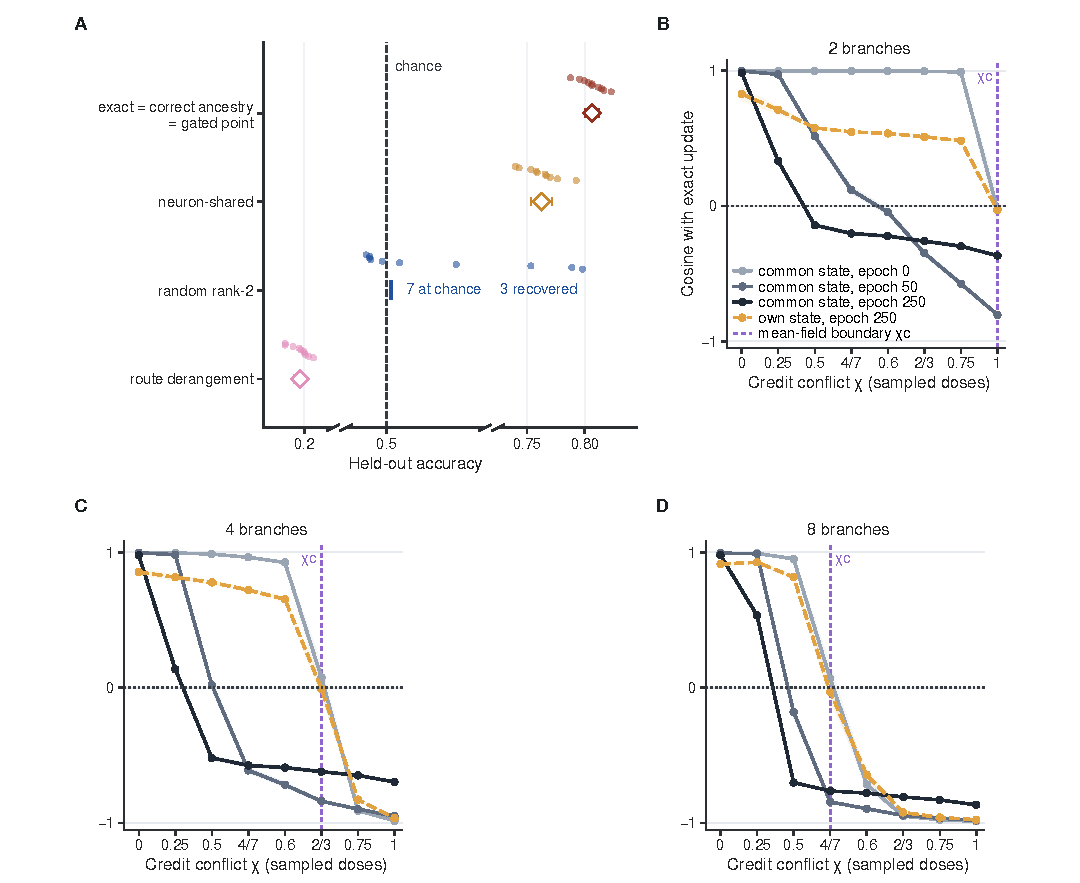
\includegraphics[width=\textwidth]{supplementary/curated/branch_conflict_controls.pdf}
\caption{\textbf{Branch-selective credit limits interference and preserves update direction.} \textbf{A}, Two-branch learning in ten paired seeds. Points show seeds; large symbols and bars are means and 95\% paired-seed bootstrap intervals. Exact path and the equivalent gated-point rule supply branch selection; the context-0 forgetting of the same cohort is drawn at the main-text type scale in main Fig.~2E. \textbf{B--D}, Shared-versus-exact gradient cosine in the separate branch-conflict experiment with two, four or eight branches. Solid curves evaluate common exact-learning states at epochs 0, 50 and 250; dashed curves evaluate the shared learner's own final state. Curves and shading use twenty paired seeds and 95\% bootstrap intervals. An exact quadratic interference calculation is given in the accompanying derivation. Learned-state geometry can depart from the initialization mean-field approximation.}
\label{fig:si_branch_conflict_controls}
\label{fig:supp_prospective_diagnostics}
\label{fig:supp_path_demand}
\end{figure}

\begin{figure}[p]
\centering
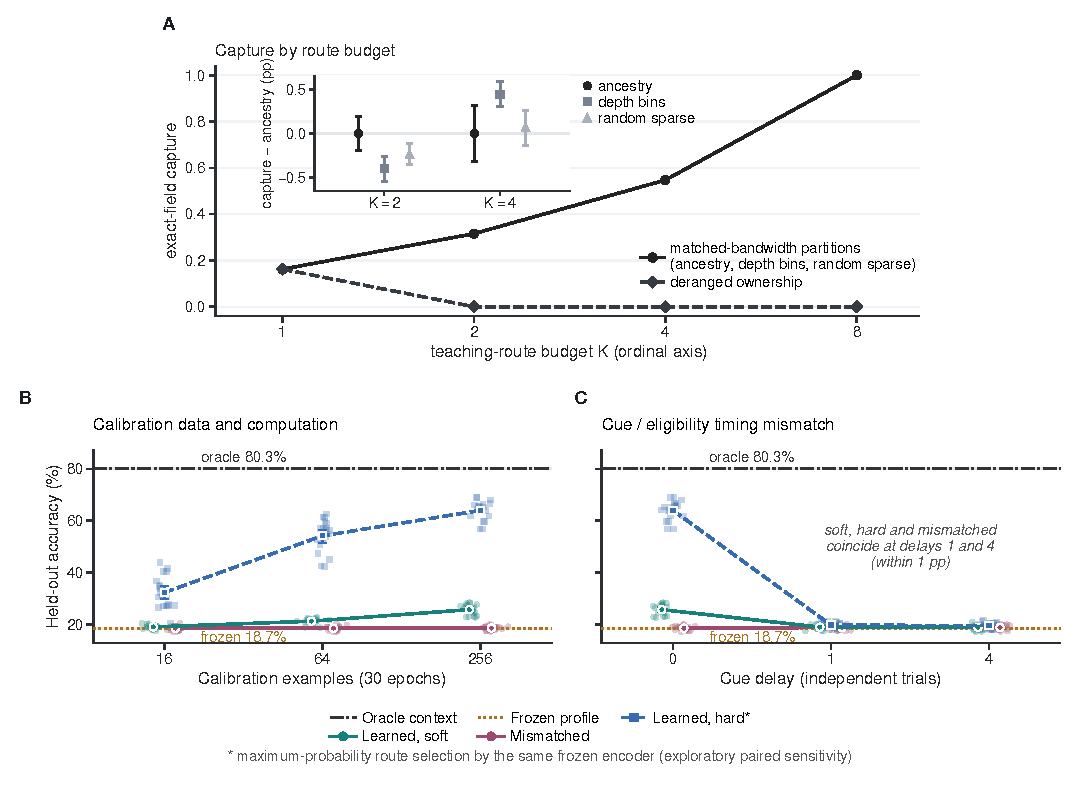
\includegraphics[width=\textwidth]{supplementary/curated/ancestry_coefficients.pdf}
\caption{\textbf{Available route span and learned route coefficients are different constraints.} \textbf{A}, Trained field capture by route budget in the eight-context factorial. Ancestry, depth and random partitions have coincident capture at matched bandwidth; derangement removes the target coordinate. Capture therefore does not explain the small ancestry-specific advantage, and capture alone does not predict trained utility: the within-seed Spearman correlation between capture and utility is about 0.82 over all budgets and 0.64 for $K<8$, and is retained numerically in Source Data. \textbf{B}, Held-out accuracy versus calibration set size (16, 64 and 256 examples) at cue-noise standard deviation 0.5 and zero delay; 30 epochs are fixed, so both data and computation increase. \textbf{C}, Cue delay at 256 calibration trials and noise SD 0.5; delays mismatch independent contexts and are measured in trials, not physiological time. In \textbf{B,C} the dashed curves marked with an asterisk use maximum-probability route selection by the same frozen encoder, an exploratory paired sensitivity specified after the soft outcomes with no encoder refit. Curves, diamonds and bars are means and 95\% paired-seed bootstrap intervals over twenty fresh analysis seeds. The cue-noise sensitivity of the same encoder is drawn at the main-text type scale in main Fig.~3F. The calibration cue and activation targets are supplied resources. No serial forward dendritic computation is present.}
\label{fig:si_ancestry_coefficients}
\label{fig:supp_partition_residual}
\label{fig:supp_local_context_encoder}
\end{figure}

\clearpage

% Curated from paper commit 7ee9157; original equations and protocol identities retained.
\section{Interaction structure, compatible trees and spatial credit}
\label{note:interactions_boolean}

\subsection{Interaction structure at fixed input-sensitivity rank}
\label{note:interaction_structure}

A tree constrains representation only if its units have restricted input access. A dense trainable leaf-input map can compensate for generic route rotations: if $W=\Phi V$, with orthonormal $K$-column routes $\Phi$, and $Q_r^{\mathsf T}H_T\Phi$ has row rank $r$, a suitable $V$ reproduces every noiseless context in the linear task of Section~\ref{note:prospective_selection}. The algebraic study below instead fixes each input to one named leaf. Its exhaustive capacity analysis was formulated after the prospective-selector outcomes and is a population diagnostic.

To impose local input access, we placed eight independent Rademacher inputs
(each equally likely to be $-1$ or $+1$) at named leaves of a binary tree.
For internal node $v$, let $u_{\mathrm L}$ and $u_{\mathrm R}$ be its
child outputs and let $a_v,b_v,c_v,d_v$ be its four trainable coefficients.
Each of the seven internal nodes computes
\begin{equation}
 u_v=a_v+b_vu_{\mathrm L}+c_vu_{\mathrm R}
       +d_vu_{\mathrm L}u_{\mathrm R}.
 \label{eq:s_multiaffine_node}
\end{equation}
Only the root is read out. Every candidate has 28 free coefficients and 14
edges, with no dense input mixing, intermediate readout or access to inputs
outside a node's subtree.
The fixed pool combines three shapes---a balanced tree, a comb and a tree
with a $3+5$ root split---with the same four predetermined leaf permutations,
giving twelve candidates. Equal edge
and coefficient counts do not imply equal cable length, latency or biological
energy cost. These signed algebraic nodes are not conductance compartments.

The primary target census contains all 105 perfect matchings $M$ and all
35 unordered four-plus-four partitions $A$ of the eight inputs:
\begin{equation}
 f_M(\bm x)=\tfrac12\sum_{(i,j)\in M}x_ix_j,
 \qquad
 f_A(\bm x)=\tfrac12\left(\prod_{i\in A}x_i+
                              \prod_{i\notin A}x_i\right).
 \label{eq:s_interaction_targets}
\end{equation}
The targets are enumerated independently of the candidate trees. Evaluating
all $2^8=256$ equally weighted inputs gives target variances 1 and $1/2$,
respectively. For the continuous derivative of each target's unique
multilinear extension,
\begin{equation}
 \E[\nabla_{\bm x}f\,\nabla_{\bm x}f^{\mathsf T}]=I_8/4.
 \label{eq:s_equal_input_sensitivity}
\end{equation}
Thus both algebraic and participation-ratio effective rank are eight, and
the complete input-sensitivity spectrum agrees. This is a property of the
target, not equality of changing model parameter-gradient or synaptic-credit
moments. Normalized MSE (NMSE) divides population squared error by the stated
target variance.

Interaction-tensor descriptions have previously been used to analyze
structured neural function classes \citep{cohen2016tensor}. The centered
constant-feature criterion below is derived for the specific local model in
Eq.~\ref{eq:s_multiaffine_node}.

\subsection{A necessary and sufficient centered-cut condition}
\label{note:centered_cut_theorem}

For each subset $U$ of input indices, define the Walsh function
$\chi_U(\bm x)=\prod_{i\in U}x_i$, with $\chi_\emptyset=1$. These
functions form an orthonormal basis under the uniform input distribution.
Writing $c_U$ for the coefficient of $\chi_U$ gives
$f=\sum_U c_U\chi_U$. If $\bm c_f$ and $\bm c_g$ collect the
coefficients of two functions $f$ and $g$, Parseval's identity gives
$\E[(f-g)^2]=\|\bm c_f-\bm c_g\|^2$. For the leaf set $S$ of an actual
subtree, reshape the target coefficients into $C_S$, with row index a subset
of $S$ and column index a subset of its complement $\bar S$. Let $C_S^\circ$ denote
this matrix after removing the row for the empty subset of $S$.

\begin{proposition}[Exact representation by a scalar multi-affine tree]
\label{prop:s_centered_tree_iff}
For a fixed binary tree with one named Rademacher input at each leaf, a target
is represented exactly by Eq.~\ref{eq:s_multiaffine_node} and a root-only
output if and only if $\operatorname{rank}(C_S^\circ)\leq1$ at every proper
subtree cut.
\end{proposition}

\begin{proof}
Every ancestor is affine in a particular child's output, and sibling inputs
are disjoint. Consequently a represented function can be written
$g=A(\bm x_{\bar S})+h_S(\bm x_S)B(\bm x_{\bar S})$. Its full cut matrix
has rank at most two; removing the empty-$S$ row leaves rank at most one.
This proves necessity.

For sufficiency, call a cut active when $C_S^\circ\ne0$. At each active
cut, choose a centered function $h_S$ whose
Fourier coefficients span the column space of $C_S^\circ$, and define
$V_S=\operatorname{span}\{1,h_S\}$. If $C_S^\circ=0$, take $h_S=0$ and
$V_S=\operatorname{span}\{1\}$. At a leaf use
$V_i=\operatorname{span}\{1,x_i\}$. The condition implies
$f\in V_S\otimes\mathcal H_{\bar S}$, where $\mathcal H$ is the complete
finite-dimensional function space on the indicated inputs.

For sibling leaf sets $L$ and $R$, the orthogonal projections onto $V_L$
and $V_R$ commute because
they act on disjoint input factors. Hence
$f\in V_L\otimes V_R\otimes\mathcal H_{\overline{L\cup R}}$.
For a non-root parent $P=L\cup R$ with nonzero centered component, write
$f=1_P\otimes A+h_P\otimes B$, with $B\ne0$. Contracting the outside
factor against a linear functional that maps $B$ to one gives
$h_P+c1_P\in V_L\otimes V_R$, where $c$ is a scalar contributed by $A$. Since the constant function also belongs to
this product space, so does $h_P$. It is therefore a linear combination of
$1,h_L,h_R,h_Lh_R$, exactly the four allowed features. Inactive parent
features are zero and cause no exception. At the root, the complete target
itself belongs to the product of its children's spaces. Induction supplies
all local coefficients and proves sufficiency.
\end{proof}

Retaining the constant feature in every subtree makes this criterion
stronger than an uncentered rank-two constraint. Let
$\mathcal T_{\rm proper}$ be the leaf sets of the tree's proper subtrees,
and let $\sigma_j(C_S^\circ)$ be the singular values in decreasing
order. The optimal low-rank approximation identity and Parseval then give
\begin{equation}
 \operatorname{MSE}(f,g)\geq
 \max_{S\in\mathcal T_{\rm proper}}
       \sum_{j\geq2}\sigma_j(C_S^\circ)^2.
 \label{eq:s_centered_cut_bound}
\end{equation}
Taking the maximum preserves a lower bound. Summing tails from overlapping
cuts instead gives a heuristic score, without the same guarantee. A positive maximum-cut bound need not equal the true optimum.
The condition applies to actual subtree cuts; the complement of a subtree
need not itself be a subtree. For the matching $(12)(34)(56)(78)$, an
even--odd root split has centered tail $0.75$, whereas the full rank-two tail
is $0.5$. For the two-quartet target with supports $1234$ and $5678$, a
five-leaf subtree $12345$ has centered tail $0.25$ despite a zero full
rank-two tail. Supplementary Fig.~\ref{fig:si_scalar_tree_capacity}
compares both bounds with fitted population error.

The proof requires ancestors to be affine in each child's output. A general
nonlinear scalar ancestor can generate higher cut rank from one scalar
feature. Neither the necessity condition nor Eq.~\ref{eq:s_centered_cut_bound}
therefore applies automatically to a tanh tree or a conductance model.

\subsection{Population fitting, complete-tree construction and depth}
\label{note:constructive_morphology}

All twelve candidates were fitted to every primary target by 32 alternating
least-squares (ALS) sweeps with four fixed random restarts. Conditional on the
other nodes, the design for one node is
$q(\bm x)[1,u_L,u_R,u_Lu_R]$, where $q$ is the derivative of the root with
respect to that node's output. The offset is the current root output minus
$q u_v$. Sweeps alternate postorder and preorder. Hidden mean/scale gauges
are normalized with exact parent compensation. Every restart and checkpoints
at 0, 2, 8 and 32 sweeps are retained: 6,720 fits and 26,880 checkpoint rows.
The endpoint is the smallest achieved NMSE among the four restarts. The difference between this endpoint and
Eq.~\ref{eq:s_centered_cut_bound} can reflect both incomplete optimization
and a loose bound, so it is not a certified optimization gap. Full-domain fitting
has no held-out generalization interpretation.

For score-based selection among the twelve fixed candidates, values within
$10^{-10}$ are treated as ties and resolved by lexicographic candidate
identifier. A separately retained summary applies this tolerance to the raw
floating-point minima without changing any fit.
The two-sweep pilot fits every candidate; the best-fixed baseline chooses a
single candidate per family in hindsight. The uniform-random baseline is its
exact candidate expectation. Family averages and paired shape/assignment
counts are descriptive censuses, with error comparisons at tolerance
$10^{-7}$ and no sampling confidence intervals over the enumerated tasks.
The lower bound is attained within this tolerance in 1,407/1,680 endpoints.
Although some restarts develop large cancelling coefficients, every case
selected by a deterministic policy has an existing equivalent restart within
$10^{-7}$ NMSE whose coefficient norm is at most 2.645752. All original fits,
including the remaining poorly conditioned case, remain included.

To search beyond the fixed pool, we used an exploratory dynamic program
over all input subsets. Let $c(S)$ be the normalized cut tail from
Eq.~\ref{eq:s_centered_cut_bound}, with zero cost at the root and leaves.
Let $b(S)$ be the smallest achievable maximum cut cost for a subtree on
leaf set $S$, with base case $b(\{i\})=0$. Then
\begin{equation}
 b(S)=\max\left\{c(S),\min_{L\dot\cup R=S}
                            \max[b(L),b(R)]\right\}.
 \label{eq:s_tree_minimax_dp}
\end{equation}
Every binary tree decomposes into one root split and two independent
children, so this recurrence covers all trees. A second pass restricts every
cut to the globally minimal threshold, then minimizes total tail, depth and
deterministic split ties. Costs are rounded to 12 decimals for numerical
ties. This corrected two-pass version is retained separately from the first
exploratory construction and agrees with exhaustive enumeration of all 945
six-input trees on four random cost tables. At a zero threshold, the theorem
makes the minimum-depth solution the shallowest exact tree in this class;
for a positive threshold only the cut score, not fitted error, is optimized.

Dominant left singular vectors of the centered cut matrices define local
scalar features, and four-feature least squares recovers each node's
coefficients. All 105 matching and 35 quartic targets reconstruct at minimum
depth three. A separate positive control uses 24 unique seeded permutations
$\pi$ of the nested target
\begin{equation}
 f_\pi(\bm x)=\tfrac12\sum_{k\in\{2,4,6,8\}}
                         \prod_{j=1}^k x_{\pi(j)}.
\end{equation}
Its rank is eight but its spectrum
$(1/4,1/4,1/2,1/2,3/4,3/4,1,1)$ differs from the primary families; it is
constant only within this control family. Every nested target requires
depth four. An independent depth-constrained recurrence gives minimum
centered-cut NMSE bound 0.146446609407 at depth at most three and zero at
depth four. All 164 constructions have NMSE below $7\times10^{-30}$ and
maximum absolute coefficient one up to rounding
(Supplementary Fig.~\ref{fig:si_scalar_tree_capacity}). The algorithm
uses the complete target Fourier tensor: these are exact-target capacity
certificates, not predictions from limited calibration data.

\subsection{Boolean interactions, scalar tree structure and conditional credit}
\label{note:boolean_morphology}

We used four-input Boolean functions to make the structural and credit
questions explicit. The complete domain comprises sixteen equally weighted
patterns. Writing $b_i=(x_i+1)/2$ for Rademacher inputs $x_i\in\{-1,1\}$, the
raw labels $y\in\{0,1\}$ are defined below. The symbols $\land$,
$\lor$ and $\oplus$ denote AND, OR and exclusive OR (XOR), respectively:
\begin{align}
 y_{\rm AND}&=b_1\land b_2\land b_3\land b_4,\qquad
 y_{\rm OR}=b_1\lor b_2\lor b_3\lor b_4,\\
 y_{\rm parity}&=b_1\oplus b_2\oplus b_3\oplus b_4,\\
 y_{\rm OR(AND)}&=(b_1\land b_2)\lor(b_3\land b_4),\\
 y_{\rm XOR(AND)}&=(b_1\land b_2)\oplus(b_3\land b_4),\\
 y_{\rm AND(XOR)}&=(b_1\oplus b_2)\land(b_3\oplus b_4),\\
 y_{\rm nested}&=b_1\land\bigl[b_2\lor(b_3\land b_4)\bigr].
\end{align}
These are specified mechanistic examples rather than a representative
sample of natural tasks. The associative AND, OR and parity families control
for claims that greater depth or a particular input grouping is inherently
necessary. Task permutations preserve a family's truth-table distribution;
comparisons between families need not preserve its input-gradient spectrum.

Every candidate has three scalar internal units, twelve trainable
coefficients and six edges. For child outputs $\ell,r$ and trainable coefficients $a,b,c,d$, each
unit computes $u=a+b\ell+cr+d\ell r$. Only the root supplies the output. All local coefficients can change during learning. There is no
additional dense decoder or access to inputs outside a unit's descendant
subtree. This is the multi-affine algebraic class of
Proposition~\ref{prop:s_centered_tree_iff}, not a positive-conductance neuron.
An independent enumeration of all fifteen unordered, rooted, full binary
trees on four labeled inputs supplies the structural analysis: three balanced
trees have depth two, and twelve comb trees have depth three. An actual subtree
cut is evaluated by removing the Fourier row for the constant function
inside that subtree and retaining the singular-value tail beyond rank one. The maximum cut tail is a lower bound
on regression MSE for the entire tree; zero tails on every actual cut are
necessary and sufficient for exact representation in this class. These
capacity statements do not by themselves establish convergence of a
particular optimizer or attainability under an additional parameter box.

We distinguish exact truth-value regression from threshold classification.
Let $\mu_y=\E[y]$ and $\sigma_y=\sqrt{\Var(y)}$ be the mean and
standard deviation over all sixteen patterns. Training targets are
$t=(y-\mu_y)/\sigma_y$. Mean squared error on $t$ therefore equals raw-output MSE
divided by $\operatorname{Var}(y)$. A predicted normalized output $\hat t$
corresponds to the raw Boolean decision
$\hat t\geq(0.5-\mu_y)/\sigma_y$. High classification accuracy does not imply
small regression error, and a positive regression lower bound does not
establish a classification impossibility. AND and OR are imbalanced: a
constant majority prediction has accuracy $15/16$. Balanced accuracy averages the true-positive rate (TPR) and true-negative
rate (TNR), $(\mathrm{TPR}+\mathrm{TNR})/2$, and distinguishes this trivial result from
accurate decisions on both classes. All sixteen truth patterns contribute
to each reported population endpoint; they are not independent biological
replicates.

\begin{proposition}[An explicit Boolean grouping obstruction]
\label{prop:boolean_xor_and}
Let $f=(b_1\land b_2)\mathbin{\mathrm{XOR}}(b_3\land b_4)$ on uniform
independent bits, and let $z=(f-3/8)/\sqrt{15/64}$. A scalar multi-affine
balanced tree grouped as $(b_1,b_3)\mid(b_2,b_4)$ or
$(b_1,b_4)\mid(b_2,b_3)$ has population NMSE at least $8/15$ for every
choice of its coefficients. The aligned grouping
$(b_1,b_2)\mid(b_3,b_4)$ represents $z$ exactly with coefficients in
$[-2,2]$.
\end{proposition}
\begin{proof}
For the crossed cut $b_1b_3\mid b_2b_4$, the raw-target centered Walsh matrix,
with nonconstant inside rows ordered as $x_1,x_3,x_1x_3$, is
\[
 C=\frac18\begin{pmatrix}
 1&1&-1&-1\\
 1&-1&1&-1\\
 -1&-1&-1&-1
 \end{pmatrix}.
\]
The columns correspond to $1,x_2,x_4,x_2x_4$. Its three orthogonal rows each
have squared norm $1/16$, so the rank-one tail is exactly $1/8$.
Dividing by $\operatorname{Var}(f)=15/64$ gives $8/15$; the other crossed
pairing is symmetric. For the aligned tree, set
\[
 u=2b_1b_2-1=\frac{-1+x_1+x_2+x_1x_2}{2},\qquad
 v=2b_3b_4-1=\frac{-1+x_3+x_4+x_3x_4}{2},\qquad
 z=\frac{1-4uv}{\sqrt{15}}.
\]
The largest absolute coefficient is $4/\sqrt{15}<2$.
\end{proof}

Exact rational Walsh coefficients were checked for all 105 family--tree pairs. All 49 zero-bound cases were reconstructed by signed Boolean slices and four-corner interpolation: AND, OR and parity admit all fifteen trees; each mixed-gate target admits one. Every normalized construction lies within $[-2,2]$, with maximum absolute coefficient $4/\sqrt{15}$. This verifies existence within the experimental box, independently of optimization.

The OR-of-AND target and the nested target each use two AND gates and one OR
gate, yet their minimum exact depths are two and three. For the nested
function, the smallest lower bound among all three balanced trees is
$(22-2\sqrt{57})/55\simeq0.12546$ NMSE; the stated comb tree is exact.
All seven functions have input-gradient rank four, but their full spectra
generally differ. This is a rank-versus-interaction example, not an
isospectral comparison between the mixed-gate families. The maximum over
cuts remains a lower bound; we do not assume every incompatible whole tree
attains it.

\paragraph{Gate coordinates illustrate conditional derivatives.}
The elementary gates can also illustrate how another branch affects a
local derivative. In raw Boolean branch-output coordinates
$u,v\in\{0,1\}$, their multilinear extensions are
\begin{align}
 F_{\rm AND}(u,v)&=uv,&\quad \partial_uF_{\rm AND}&=v,\\
 F_{\rm OR}(u,v)&=u+v-uv,& \partial_uF_{\rm OR}&=1-v,\\
 F_{\rm XOR}(u,v)&=u+v-2uv,& \partial_uF_{\rm XOR}&=1-2v.
\end{align}
The other branch thus gates a derivative's magnitude or sign in these
canonical coordinates. The XOR-of-AND diagram illustrates this dependence
and a specific input-grouping constraint. Its gate labels are explanatory;
the learned units are not constrained to remain Boolean gates or to preserve
that representation. A broadcast learner can change internal coordinates,
so the derivative diagram is not a proof that broadcast cannot learn the
task. Positive affine normalization of the raw target changes derivative
scale but not these signs. Actual learned update fields and finite-training
outcomes require the separate experimental comparisons below.

\paragraph{Frozen learning comparisons.}
Four candidate trees were tested: the three balanced pairings and the comb
$b_1\mid[b_2\mid(b_3,b_4)]$. These are four of the fifteen trees in the independent
capacity analysis. Each seed applied one common physical input permutation
to both the semantic task variables and candidate leaves. Per-family streams
supplied initialization, a 256-observation training cache, 1,024 independent
test observations and minibatch indices. All paired tree, optimizer, credit
and rate conditions shared these streams within family. Data were drawn
uniformly with replacement from the sixteen patterns; training and test
labels received independent Gaussian noise of SD 0.15 in normalized-target
units. Independent draws could repeat the same input pattern.

Every coefficient began from an independent mean-zero Gaussian with SD 0.5,
except zero biases; no target gates, coefficients or exact-construction
weights were used. Initial weights and every subsequent update were clipped
to $[-2,2]$. Training used 2,048 updates, minibatches of 32, and gradient norm
clipping at ten. Exact credit multiplied each local eligibility by the
current complete path derivative. Broadcast set the two nonroot internal
sensitivities to one; root sensitivity remained one under both rules. All
twelve coefficients were trainable. Stochastic gradient descent (SGD) and Adam were tested separately;
Adam used $(\beta_1,\beta_2)=(0.9,0.999)$ and $\epsilon=10^{-8}$.

Five development seeds (2026110--2026114) selected a rate separately for each
optimizer and rule from 0.003, 0.01 and 0.03, minimizing mean final clean
population NMSE over all seven families and four trees. Ties within
$10^{-12}$ selected the smaller rate. Adam selected 0.003 for exact credit
and 0.01 for broadcast; SGD selected 0.03 and 0.01, respectively. These choices were recorded with cryptographic hashes before twenty new
seeds (2026210--2026229), which
retained all three rates. The resulting 6,720 fresh fits supplied 53,760
records at updates 0, 1, 16, 64, 256, 512, 1,024 and 2,048. An implementation check using seed 2026000 exercised all 336 conditions
and was excluded from inference. These seeds vary initialization,
permutation and sampled noisy data for seven fixed logical templates;
they do not sample new Boolean function families.

The primary endpoint was clean population NMSE evaluated on all sixteen
patterns. No sampled test variance or observed class-frequency denominator
entered this endpoint. Noisy-test NMSE, raw threshold accuracy and balanced
accuracy were secondary. Gradient cosines compare the delivered and exact
aggregate clean-population gradients at each learner's own trained state,
before clipping or optimizer transformation; they are not mean per-example
cosines or common-state comparisons between separately trained rules.

Two primary Adam contrasts concerned XOR-of-AND: the mean of the two crossed
balanced-tree errors minus aligned-tree exact-credit error, and broadcast
minus exact error on the aligned tree. The latter compares the
prespecified development-selected recipes, not identical learning rates.
Ten thousand resamples of twenty paired seed blocks supplied two-sided
Bonferroni-adjusted 97.5\% intervals for these two contrasts. A positive
adjusted lower limit and mean improvement of at least 0.01 NMSE were both
required. Other task, optimizer and common-rate contrasts have descriptive
pointwise 95\% intervals.

The grouping improvement was 0.56317 NMSE $[0.54914,0.58275]$, satisfying both
primary criteria. The credit difference was 0.002507
$[0.001780,0.003318]$: its adjusted interval excluded zero, but it did not
meet the prespecified 0.01-NMSE mean-effect margin. Both recipes learned the
aligned XOR-of-AND task well and classified all sixteen patterns correctly
in every fresh seed. All three same-rate Adam credit differences
were also below 0.003 NMSE. The low-rate SGD contrast had a wide interval and
is retained. The larger parity credit differences are descriptive outcomes
of a prespecified control task, not primary discoveries. Neither the gate
illustration nor these observations establish an impossibility theorem for
broadcast learning, or show that a particular change of internal coordinates
caused its success. Full-rate outcomes, constant-mean and random-candidate
references, clipping records, weights and source/selection hashes are retained
under \texttt{source\_data/boolean\_morphology}.

% Explicitly post hoc, specified after reviewing the fresh Boolean results.
\paragraph{Post hoc diagnostic of local target information.}
After examining the fresh learning outcomes, we asked how much target
information was available within each proper input subset $S$. In this
diagnostic, $f$ denotes a raw Boolean target, $z=(f-\E[f])/\sqrt{\Var(f)}$
its normalized version, and $\widehat f_U$ its Walsh coefficient on input
subset $U$. The squared $L^2$ norm below averages over the uniform input
distribution. We defined
\[
 P_S=\big\|\mathbb E[z\mid x_S]\big\|_{L^2}^2
 =\frac{1}{\operatorname{Var}(f)}
   \sum_{\emptyset\ne U\subseteq S}\widehat f_U^{\,2}.
\]
We cross-checked all ninety-eight task--subset values by exact rational
evaluation of conditional means on the full truth table. Parity4 has $P_S=0$
for every proper subset. XOR-of-ANDs instead has $P_S=1/5$ for every two-input
subset, including compatible and crossed pairs. Thus this diagnostic quantifies
accessible lower-order target information rather than grouping compatibility.

Let $F$ denote the model's normalized prediction. At fixed parameters, a
local eligibility $e_S(x_S)$ at a nonroot subtree is a
function only of that subtree's inputs. Conditional expectation gives
$\mathbb E[ze_S]=\mathbb E[\mathbb E[z\mid x_S]e_S]$; when $P_S=0$, the direct
target contribution to the population broadcast update
$\mathbb E[(F-z)e_S]$ vanishes. This identity does not imply an inability to
learn: label-dependent changes in root coefficients can subsequently affect
$F$, and finite training samples and stochastic updates need not exhibit exact
population cancellation. The diagnostic was added after observing the learning
results and did not change the training protocol or its predeclared criteria.
\subsection{Learning compatible trees with exact and restricted credit}
\label{note:morphology_credit_learning}

To separate credit assignment from uncertainty in structure estimation, this experiment supplied a tree compatible with the full target. Three development seeds and twenty fresh seeds generated independent signed and permuted matching, quartet and nested-interaction targets. The complete target Fourier tensor supplied a compatible tree through the preceding dynamic program; no target-derived coefficients initialize learning. An independent permutation of leaf labels preserved the exact shape, 28 coefficients and 14 edges. Chance compatible permutations were retained. The primary matching and quartet families retained identical input-sensitivity spectra, while the nested family had the previously stated anisotropic spectrum.

All seven internal units initialized their non-bias coefficients independently from $\mathcal N(0,0.5^2)$, with zero biases. The same initial coefficients, training cache and minibatch draws were used across paired assignments, credit rules and optimizers. Local features were $(1,u_L,u_R,u_Lu_R)$ and the exact path derivative $q_v=\partial u_{\rm root}/\partial u_v$ supplied credit. Exact gradients agreed with central finite differences for every coefficient in all three families. Root sensitivity was one under every rule. The six nonroot internal units received either the exact field, a unit root broadcast, the orthogonal projection onto a single constant profile, or the projection onto two proximal-subtree indicator profiles. A size-matched permutation of the latter profiles served as a control. All projected coefficients were computed from the current exact field and are therefore oracle coefficients; the experiment did not learn a circuit estimator for them.

Training used 2,048 independently sampled Rademacher examples with output noise SD~0.15 and 1,024 minibatch updates of size~64. The gradient corresponded to half-MSE divided by the known clean target variance. Stochastic gradient descent (SGD) and Adam ($\beta_1=0.9,\beta_2=0.999$, $\epsilon=10^{-8}$) each tested learning rates 0.003, 0.01 and 0.03. Update gradients were clipped at norm~10 and parameters projected to $[-2,2]$, which contains all exact constructions. Every clipping/projection count was recorded. These are constrained finite-horizon training results, not estimates of unrestricted optimization optima.

A separate learning rate for each optimizer and rule minimized mean development population NMSE over all families and both assignments. A common rate per optimizer was also selected on development. All choices were recorded with cryptographic hashes before any fresh fit; all three rates remain in the released outcomes. Every SGD rule selected the upper tested rate, so the grid does not establish its best attainable optimizer setting. The independent test set contained 4,096 examples with fresh SD~0.15 output noise. Test NMSE, normalized by the clean target variance, was primary; noiseless population NMSE on all 256 inputs was secondary. Evaluation at steps 0, 1, 16, 64, 256 and 1,024 retained 21,600 checkpoint rows from 3,600 fresh fits. The endpoints at the development-selected rates contained 1,200 fits. No run was excluded. Ten thousand bootstrap samples of twenty whole paired seed blocks were drawn for pointwise 95\% intervals, averaging families within seed for pooled contrasts. Multiple subgroup intervals are descriptive, not separately multiplicity-adjusted discoveries.

Exact credit strongly improves learning of compatible quartet and nested targets under both frozen optimizer recipes. Broadcast is already effective for matching targets and outperforms exact credit there under SGD. Restricted two-subtree projections help in some Adam conditions but do not consistently beat shuffled profiles, and have essentially no pooled advantage over broadcast under SGD. For compatible trees trained with exact credit and Adam, mean test NMSE was 0.0329; permuting the input labels increased it to 0.6080. At the common Adam rate 0.01, the compatible exact/broadcast averages remain 0.0329/0.5973. Supplementary Fig.~\ref{fig:si_oracle_profile_credit} reports the full family, optimizer, profile, assignment and rate controls. Numerical outcomes and source/selection hashes are in \texttt{source\_data/morphology\_credit/}.
\subsection{Matched fixed-profile learning and credit-field geometry}

This experiment separates forward compatibility, spatial profile calibration and learning. This matched cohort retains the seven-unit model, 28 coefficients and compatible constructions above, specializing hierarchical tensor representations to scalar messages \citep{hackbusch2009tensor,grasedyck2010hierarchical}. Pairwise and quartic targets share a balanced tree and seed-specific leaf permutation. Independent coefficient signs have magnitude one-half; both input moments equal $I_8/4$, while target variances are one and one-half. The nested target uses its separate compatible tree and anisotropic spectrum.

Let $q_n(x)=\partial u_0/\partial u_n$ be the exact path derivative for unit $n$, and let $\delta(x)$ be the scalar derivative of normalized half-squared error with respect to root output. Local coefficient eligibilities are $1,u_L,u_R,u_Lu_R$. Exact credit multiplies these by $\delta q_n$. Unit broadcast replaces $q_n$ by one. An initially calibrated profile uses $a_n=256^{-1}\sum_x q_n(x)$ over 256 unlabeled initialization examples, then keeps $a_n$ fixed. The sign control retains only $\operatorname{sign}(a_n)$. Profiles require no target labels. Learning-rate choices are separate from the profile calculation. Fixed positive coordinate scaling largely cancels under Adam, so calibrated and sign-only Adam trajectories are expected to be nearly identical; they are not independent mechanistic confirmations.

The protocol preceded three disjoint development seeds, with the same rate grid for each rule and optimizer. Separate rule-specific and common rates minimized final validation NMSE across families and were sealed before twenty paired fresh seeds. Matching/quartic conditions share initialization, calibration, examples, noise and minibatches. The Adam primary contrast is the quartic-minus-pairwise difference in initial-profile-minus-exact held-out error. All selected/common-rate unions are retained: 432 development, 1,200 fresh fits, and 48 excluded short checks.

Algebraic train/validation/test sizes are 2,048/1,024/4,096; minibatches have 64 examples. Nonbias coefficients initialize independently with Gaussian SD 0.5 and biases zero. Both SGD and Adam test 0.003/0.01/0.03; Adam uses $(0.9,0.999)$ and $\epsilon=10^{-8}$. Fits retain norm clipping ten, box $[-2,2]$, all contacts and steps 0, 1, 16, 64, 256, 512 and 1,024. Label-noise SD 0.15 gives NMSE floors 0.0225 for matching/nested and 0.045 for quartic; normalized half-MSE uses each family's clean variance. All poorly fitted exact endpoints remain. Pointwise intervals use 10,000 whole-seed draws.

The separate positive-conductance comparison uses the compatible sixteen-parameter teacher of Section~\ref{sec:conductance_grouping_bridge}, not the algebraic quartic target. Data sizes are 1,024/1,024/4,096 without label noise, box $[-5,5]$, SGD rates 0.001/0.003/0.01 and Adam rates 0.003/0.01/0.03.

For each saved state, let $Q$ have one row per evaluation example and six columns containing $q_n$. For a dictionary $A$, energy capture is $\|QP_A\|_F^2/\|Q\|_F^2$, where $P_A$ is its orthogonal projector. The best fixed rank-one profile is the leading right singular vector of $Q$, with capture $\sigma_1(Q)^2/\sum_j\sigma_j(Q)^2$. Its profile and per-example amplitudes are oracle fits. The uncentered second moment is $C=Q^{\mathsf T}Q/N$, and participation-ratio effective rank is $(\operatorname{tr}C)^2/\operatorname{tr}(C^2)$. We additionally evaluated unit broadcast, the fixed initial profile, ancestry spans, full-rank capture, and loss-error-weighted fields $\operatorname{diag}(\delta)Q$. The latter has its own optimal profile; applying the path-optimal profile after error weighting answers a different question.

Eligibility-weighted reconstruction multiplies exact and projected path fields by their local coefficient features before comparing parameter updates. Site-normalized spectra divide each path coordinate by its root-mean-square magnitude, exposing sensitivity to fixed coordinate scaling. Raw capture energies are not invariant to arbitrary hidden-unit rescaling. At identical weights and inputs, $Q$ is independent of the target; a scalar residual also cancels from normalized per-example projection capture whenever it is nonzero. Eighty common-state relabeling controls verify that identity. These diagnostics characterize learned-state geometry, rather than infer a task-only credit rank at initialization.

An independent saved-state audit checked 20,160 metrics and 120 matching--quartic pairing identities. For the earlier cohort whose states had not been stored, replay reconstructed 3,600 checkpoints and matched 28,800 archived metrics within $9\times10^{-16}$. These are reconstructed states, distinguished from the directly archived matched-cohort checkpoints. Source Data retain the complete numerical audit.

The positive-conductance comparison uses the prior compatible teacher across three paired input permutations and the same credit definitions. It does not implement the algebraic quartic target. All four rules learn it accurately with Adam; exact credit has mean NMSE $9.39\times10^{-6}$, compared with $1.35\times10^{-6}$ for the fixed-profile controls. Positive path derivatives make sign and unit broadcasting identical. Both models' local updates were independently checked by finite differences. Protocols, selections, checkpoints, full trajectories, numerical audits and scripts are supplied in \texttt{source\_data/credit\_rule\_bridge/}, \texttt{source\_data/credit\_resolution\_bridge/} and their corresponding script directories.
\subsection{Balanced extension of the matched credit-rule comparison}
\label{sec:credit_rule_extension}

After examining the released 1,024-update outcomes, we froze and committed a longer-budget protocol before running any extended trajectories. This is a protocol-led extension of previously observed seed blocks, not a fresh confirmatory cohort. All 720 algebraic trajectories were retained: twenty seed blocks, three task families, four delivery rules, Adam and SGD, and the union of the original development-selected and common rates. Matching and quartic targets retain the same balanced tree, initialization and example streams; nested targets retain their separately compatible trees. No rates were retuned.

Every trajectory was replayed from initialization and run for exactly 16,384 updates, preserving examples, minibatches, local rules, gradient clipping and coefficient bounds $[-2,2]$. All original checkpoint arrays, numerical curves and diagnostics through 1,024 updates reproduced. Additional observations occurred every 256 updates after 1,024. Terminal outcomes at 1,024, 4,096, 8,192 and 16,384 updates preserve the original endpoint definition. Secondary states minimized validation NMSE over the declared observations within each budget, with ties assigned to the earlier checkpoint. Test and full-domain population errors were used only for reporting. Independent recomputation of all 5,760 budget-outcome rows from saved weights reproduced test, validation and population NMSE exactly; all 2,880 validation-only selections were checked.

All twenty selected-rate Adam exact quartic fits reached the test noise floor by 4,096 updates, resolving three slow 1,024-update outcomes. By that budget exact pairwise credit also had slightly lower mean error than the initial profile, with eighteen of twenty exact wins. The original pairwise mean ordering reflected slow exact seeds, despite exact credit winning fifteen of twenty initial pairs. Compact endpoints are in Supplementary Table~\ref{tab:credit_rule_extension_endpoints}.

At 16,384 updates, the selected-rate calibrated-minus-exact quartic-minus-pairwise interaction was 0.9516 (95\% paired interval, 0.8829--1.0123) for terminal states and 0.7903 (0.6915--0.8797) for validation-selected states. Corresponding common-rate effects were 0.9028 and 0.7952. All four contrasts were positive in every seed. Intervals use 10,000 whole-seed bootstrap draws and are descriptive because the original outcomes were already known.

The comparisons remain constrained by time, parameter bounds and historical rates. Every selected-rate Adam initial-profile trajectory had contacted a coefficient bound by 16,384, whereas none of the corresponding exact trajectories had. Validation-selected initial-profile states still had substantial quartic and nested error, and the full record retains clipping and bound events. Extended exact-trained path fields remained almost one-dimensional for pairwise targets but multidirectional for quartic and nested targets; the original main-figure capture analysis is retained unchanged. These results strengthen the fixed-budget contrast and explain the slow exact runs, without proving that a bounded fixed profile fails under every optimizer or that full compartment resolution is uniquely necessary.

\subsection{Noise sensitivity with inherited learning rates}
\label{sec:noise_sensitivity}

For a homogeneous multilinear polynomial $f=\sum_{|U|=d}c_U\chi_U$
under independent symmetric binary inputs, orthogonality gives
$\operatorname{Var}(f)=\sum_Uc_U^2$ and
$\E\|\nabla_xf\|^2=\sum_U|U|c_U^2=d\operatorname{Var}(f)$.
Matching pairwise and quartic derivative spectra therefore forces unequal
target variances, one and one-half. Identical absolute label noise is not
identical relative noise. We tested this alternative explanation directly.

An internally specified post-review protocol used twenty additional paired
seed blocks, disjoint from the original bridge cohort. Both targets retained
the same seven-unit tree, leaf permutation, initial coefficients, input
matrices, standardized noise, calibration examples and minibatch indices
within each seed. The three label-noise conditions were SD 0.15,
SD zero, and SD $0.15\sqrt{\operatorname{Var}(f)}$. The last condition gives
relative noise variance 0.0225 for both targets. Fixed and relative noise
are consequently identical for the pairwise target, providing an exact
implementation check rather than independent observations.

We retained the original Adam rates selected on the earlier development
split: 0.003 for exact and unit broadcast, 0.01 for calibrated and sign-only
broadcast, plus common rate 0.003 for every rule. Rates were not selected
again for any noise condition. Each task/noise combination therefore had
six unique rule--rate trajectories. Twenty seeds, two tasks and three noise
conditions gave 720 trajectories, all run to 16,384 updates with the original
batch size 64, parameter bounds $[-2,2]$ and norm-ten clipping. Training,
validation and test sets contained 2,048, 1,024 and 4,096 examples;
calibration used 256 unlabeled examples. Every condition used the same Adam
moment coefficients and numerical stabilization as the original bridge.

The primary endpoint was the quartic-minus-pairwise difference in the
calibrated-minus-exact error gap, evaluated without noise over all 256 input
patterns. This removes finite test-sample and test-noise variation while
retaining the effect of training noise. All fixed checkpoints, noisy-test
outcomes, unit/sign-only controls, clipping and bound contacts are retained.
Whole-seed bootstrap intervals use 10,000 resamples; other checkpoints and
common rates are descriptive sensitivities. No test outcome selects a
checkpoint or learning rate.

At 16,384 updates the primary difference was 0.963 with fixed absolute noise,
1.030 without noise and 1.007 with matched relative noise. Each was positive
in all twenty seeds; the common-rate differences were 0.911, 0.916 and
0.911, also positive in all seeds (Table~\ref{tab:noise_sensitivity}).
Thus the tested fixed-profile deficit persists when the noise imbalance is
removed. This does not establish noise-optimal settings, unconstrained
convergence or a requirement for all six exact channels. The seed-level
tables include every outcome. Independent forward replay of the 1,024- and
16,384-update checkpoints agreed within $10^{-10}$ with clean-domain
outcomes. Code and protocol identities are in
\texttt{noise\_controls\_provenance.json}; complete curves and contrasts are
under the same prefix in \texttt{source\_data/curated\_publication/}.

\begin{figure}[p]
\centering
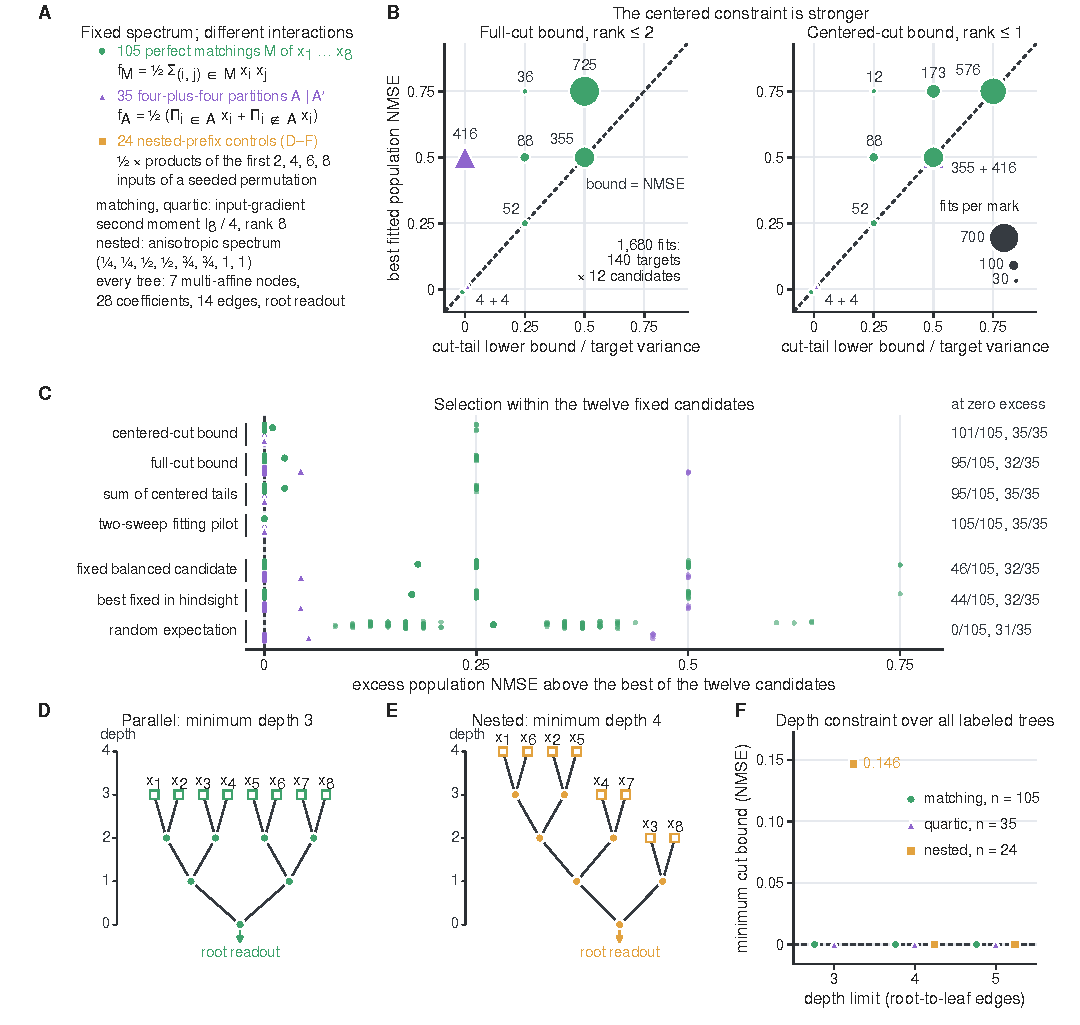
\includegraphics[width=\textwidth]{supplementary/curated/scalar_tree_capacity.pdf}
\caption{\textbf{Interaction structure constrains scalar trees at matched input spectra and resources.} \textbf{A}, Exhaustive pairwise matching and two-quartic target families on eight independent binary inputs and the 24 nested-prefix controls (one anisotropic spectrum); the panel is the key of the sheet: green filled circles, the 105 matching targets; purple filled triangles, the 35 quartic targets; amber filled squares, the 24 nested controls; grey dashed rules are references (equality in \textbf{B}, zero in \textbf{C} and \textbf{F}). \textbf{B}, Full rank-two and centered rank-one cut-tail lower bounds versus achieved population NMSE; mark area is proportional to the number of fits at that point, printed beside each mark (1,680 fits, 4--725 per point; marks of at most 18 fits sit at a 3.2 pt floor; area key, 30, 100 and 700 fits). Marks of both families at one point are superposed, the smaller on top, with one label for both counts (355 + 416 at bound 0.5, centered); the two four-fit marks at the origin touch along the equality rule. \textbf{C}, Excess NMSE above the best fitted candidate in the fixed pool of twelve: large marks, family means over the 105 matching (upper sub-row) or 35 quartic (lower sub-row) targets; small translucent dots, the per-target values, jittered vertically; the right-hand column counts targets at exactly zero excess. Above the gap, the four bound and pilot selectors; below it, the fixed balanced-shape candidate (mean excess 0.181 matching, 0.043 quartic), best-fixed selection in hindsight and the uniform random expectation. Under the centered-cut bound 101 of 105 matching and all 35 quartic targets have zero excess, so the matching mean 0.0095 rests on four targets at 0.25. \textbf{D}, Tree returned for the first enumerated matching, a depth-three parallel construction. \textbf{E}, First seeded nested-prefix control tree, of minimum depth four. Inputs enter at the top and the root is read out at the foot, as in main Fig.~4A: open squares, input leaves; filled discs, multi-affine nodes; both trees at one level pitch against the shared depth ruler. \textbf{F}, Minimum possible maximum centered-cut bound over all labeled binary trees at depth limits of 3, 4 or 5 edges (ordinal axis; families side by side at each limit), identical within each family ($n$ = 105, 35 and 24): zero at every limit for matching and quartic targets; 0.146 at depth limit 3 and zero at 4 and 5 for nested controls; the dashed rule marks zero.}
\label{fig:si_scalar_tree_capacity}
\label{fig:supp_interaction_structure}
\label{fig:supp_constructive_morphology}
\end{figure}

\begin{figure}[p]
\centering
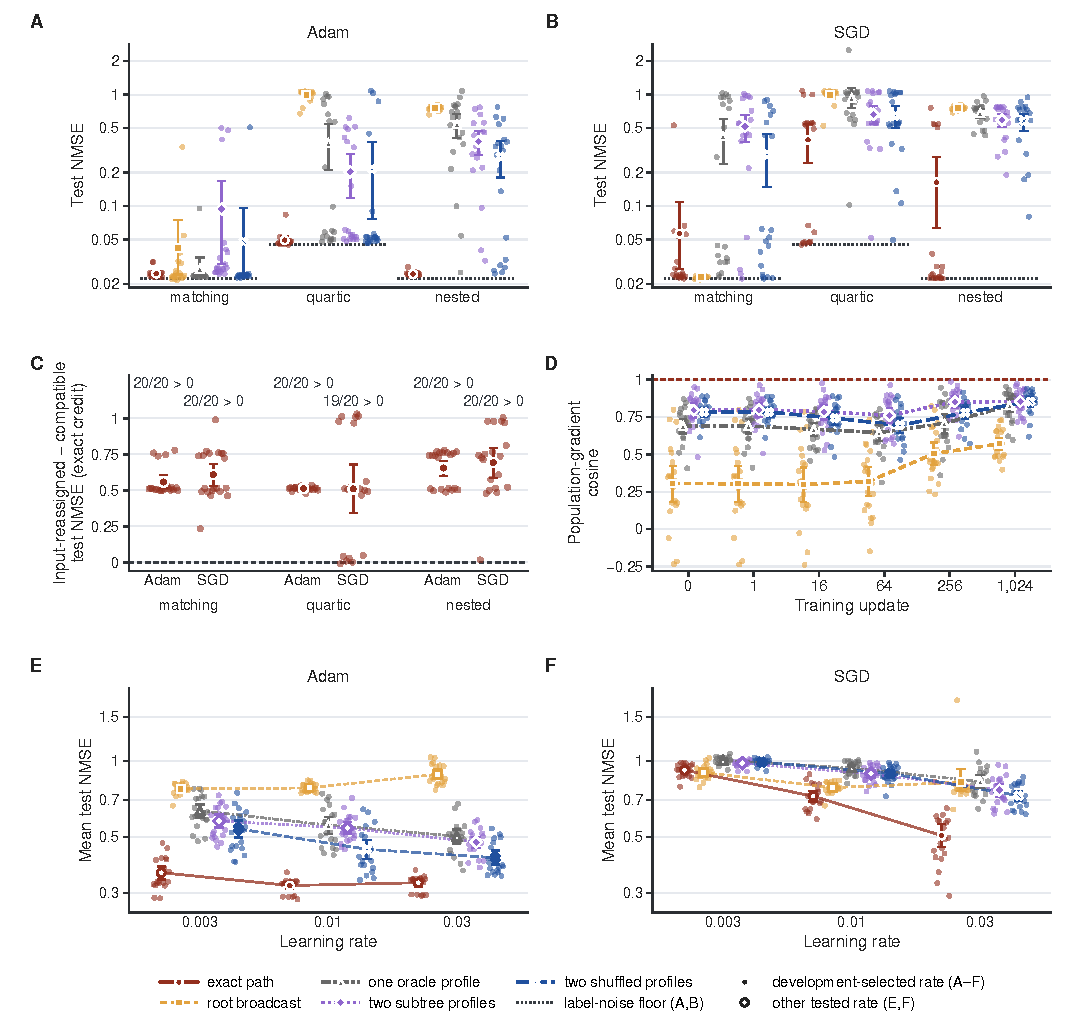
\includegraphics[width=\textwidth]{supplementary/curated/oracle_profile_credit.pdf}
\caption{\textbf{Task-dependent credit requirements in bounded multi-affine trees.} \textbf{A,B}, Final test normalized mean squared error (NMSE) on oracle-compatible trees under Adam and stochastic gradient descent (SGD), respectively. Exact path (red-brown, circle, solid line), root broadcast (amber, square, dashed), one oracle profile (grey, triangle, dash-dot), two subtree profiles (violet, diamond, dotted) and two shuffled profiles (blue, cross, long dash). The NMSE axis is logarithmic; small translucent points are the twenty individual seeds behind each mean, and dotted rules spanning only the family they apply to mark the known label-noise floors: 0.0225 for matching and nested tasks and 0.045 for quartic tasks. \textbf{C}, Paired exact-credit NMSE increase after reassigning the leaf inputs (not the shuffled-profiles rule) while preserving tree shape and parameter count, for Adam and SGD (axis labels); every mark is the exact-path red-brown, the twenty paired seed differences are drawn behind each mean, the number of positive differences out of twenty is printed above each strip, the dashed rule is zero, and the Adam quartic interval (0.507--0.517), narrower than its marker, is printed beside the point. \textbf{D}, Adam gradient cosine between the exact and delivered aggregate clean-population updates, evaluated at each rule's own trained state after 0, 1, 16, 64, 256 and 1,024 updates (equally spaced ordinal axis), each seed averaging the three task families before aggregation; the exact-path cosine is 1 by definition and is the dashed red-brown reference, not a series; the fan behind each mean is the twenty per-seed values. Points and whiskers in \textbf{A--F} are means and pointwise 95\% intervals from 10,000 whole-seed bootstrap draws, twenty fresh seeds per family. \textbf{E,F}, Final NMSE at the three tested learning rates 0.003, 0.01 and 0.03 (categorical positions), averaged over both compatible and reassigned input assignments and all three families, on one common logarithmic NMSE axis; each point carries its twenty per-seed means and whisker, and thin connectors in each rule's dash pattern join the three rates. Filled markers, the development-selected rate of each rule and optimizer (used in \textbf{A--D}); open markers, the other tested rates. The Adam strips of \textbf{C} are main Fig.~4H's contrast (``matching'' is ``Pairwise'' there).}
\label{fig:si_oracle_profile_credit}
\label{fig:supp_morphology_credit}
\end{figure}

\begin{figure}[p]
\centering
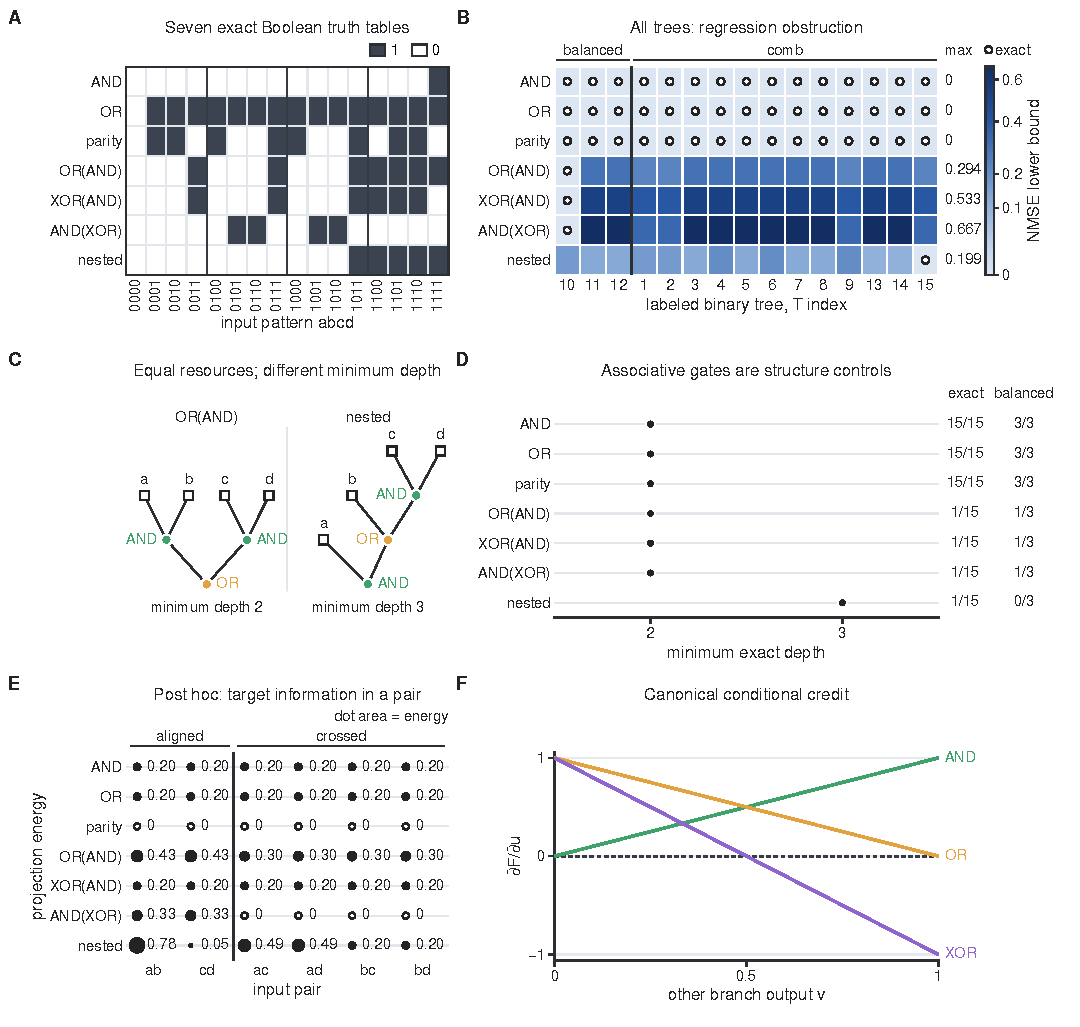
\includegraphics[width=\textwidth]{supplementary/curated/boolean_capacity.pdf}
\caption{\textbf{Boolean interactions distinguish structure, depth and canonical credit.} \textbf{A}, Truth tables of seven four-input templates on the sixteen equally weighted patterns (white, 0; slate, 1); columns are $abcd$ in numeric order, $a$ the most significant bit, hairlines between groups of four sharing $a$ and $b$. Mixed targets: \((a\land b)\lor(c\land d)\), \((a\land b)\mathbin{\mathrm{XOR}}(c\land d)\), \((a\mathbin{\mathrm{XOR}}b)\land(c\mathbin{\mathrm{XOR}}d)\) and nested \(a\land[b\lor(c\land d)]\). \textbf{B}, Centered-cut normalized-mean-squared-error (NMSE) regression lower bounds for all fifteen labeled binary trees (twelve coefficients, six edges); the rule separates the balanced (depth-two) trees T10--T12 from the twelve comb trees. The colour ramp is a power mapping (exponent 0.6) of the bound from a faint tint (zero cells palest); the nested row is positive on every tree but T15 (0.105--0.199); row maxima are printed at right. Open rings (a marker, not a bound) mark the 49 exactly representable family--tree pairs, certified with coefficients in $[-2,2]$ (largest $4/\sqrt{15}$; T indices and cut sets in Source Data). \textbf{C}, OR-of-AND and nested each use two AND gates and one OR gate (node colours as in \textbf{F}; inputs above, output below) but need minimum exact depths two and three. \textbf{D}, Minimum exact depth (ordinal axis, 2 or 3); the columns count exactly compatible trees among all fifteen (the ring counts of \textbf{B}) and among the three balanced: 15/15 and 3/3 for AND, OR and parity, 1/15 and 1/3 per mixed-gate target, 1/15 and 0/3 for nested. \textbf{E}, Post hoc target-projection energy $\|\mathbb E[z\mid x_S]\|^2$ of all seven families on the six two-input subsets, normalized target $z$: dot area is proportional to the energy, values printed beside the dots, exact zeros are open rings, and the rule separates aligned pairs ($ab$, $cd$) from crossed. XOR-of-AND has $1/5$ on every pair; parity has zero on every proper subset (all fourteen per family in Source Data). \textbf{F}, Canonical derivatives \(\partial F/\partial u\) for left-branch output \(u\) against right-branch output \(v\): AND, \(v\); OR, \(1-v\); XOR, \(1-2v\); dashed rule, zero. Green, amber and violet in \textbf{C,F} name the gates AND, OR and XOR, not bound values; \textbf{D,E} are drawn in ink only. Panels are exhaustive analytic diagnostics (no sampling error bars): positive bounds concern truth-value regression, not threshold classification; \textbf{E} is local target information, predicting neither grouping compatibility nor broadcast-learning failure; \textbf{F}'s raw derivatives need not survive training and imply no learning outcome; assumptions: Supplementary Note~\ref{note:boolean_morphology}.}
\label{fig:si_boolean_capacity}
\label{fig:supp_boolean_theory}
\end{figure}

\begin{figure}[p]
\centering
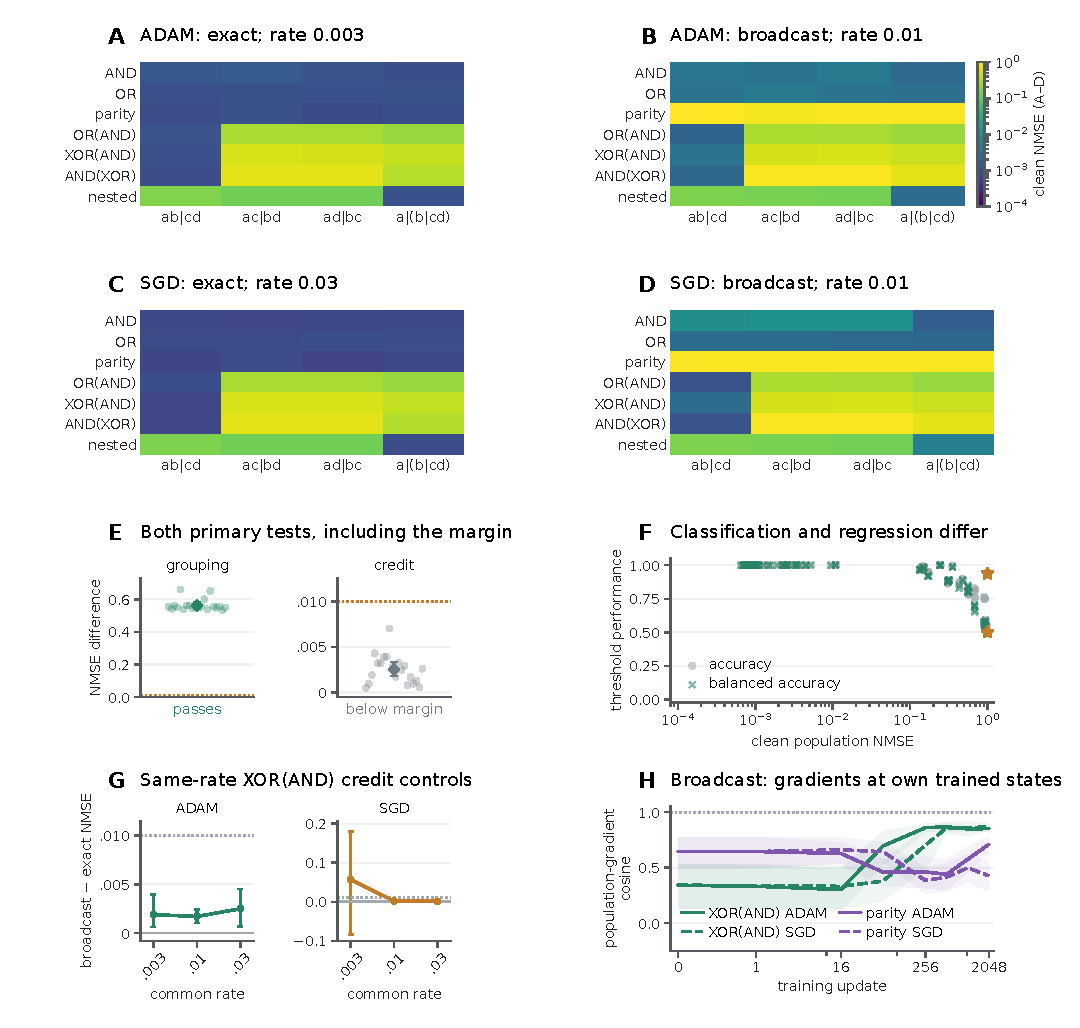
\includegraphics[width=\textwidth]{supplementary/curated/boolean_learning.pdf}
\caption{\textbf{Boolean grouping benefit and a small primary credit effect under frozen recipes.} \textbf{A--D}, Clean population normalized mean squared error (NMSE), twenty-seed means, for seven target families (rows, labelled at \textbf{A,C}) and four trees (three balanced groupings and the comb a|(b|cd)) under Adam (\textbf{A,B}) and stochastic gradient descent (SGD; \textbf{C,D}) with exact (\textbf{A,C}) or broadcast (\textbf{B,D}) credit, on one logarithmic colour scale (key at right). Rates (0.003, 0.01, 0.03 and 0.01 in \textbf{A--D}) were selected per optimizer and rule on five development seeds; per-cell 95\% intervals are in Source Data. \textbf{E}, Prespecified Adam XOR-of-AND contrasts: grouping, the crossed-tree mean (ac|bd, ad|bc) minus the aligned ab|cd under exact credit; credit, broadcast minus exact on ab|cd. Dots (green, as XOR-of-AND in \textbf{G,H}), twenty paired seed differences; rules and whiskers, means and Bonferroni-adjusted 97.5\% intervals (grouping 0.549--0.583); amber dotted, the 0.01-NMSE mean-effect margin. The grouping axis is broken, zero and the margin in its foot strip; the credit subpanel has its own y range and a solid zero rule. Grouping passes both criteria, credit does not; both rules classify all sixteen patterns perfectly in every seed. \textbf{F}, Accuracy (gray circles) and balanced accuracy (blue crosses) versus NMSE for the 112 conditions at raw-output threshold 0.5; sixty overprint at 1.00 on both. Amber stars, the AND/OR constant-majority references (NMSE one, accuracy $15/16$, balanced accuracy $1/2$). \textbf{G}, Same-rate broadcast-minus-exact contrasts on the aligned XOR-of-AND tree, Adam (left) and SGD (right): dots, twenty paired seed differences per common rate (logarithmic axis); rules and whiskers, joined across rates, means with descriptive 95\% intervals; amber dotted, the 0.01 margin; dark solid, zero. The SGD y axis is symmetric-log (linear within $\pm 0.002$) to keep the rate-0.003 seed differences ($-0.94$ to $0.61$) in view. \textbf{H}, Broadcast gradient cosine on the aligned balanced tree for XOR-of-AND (green) and parity (violet); solid lines, filled markers Adam; dashed lines, open markers SGD; on all sixteen clean patterns at each learner's own state before clipping or optimizer transformation; eight checkpoint markers on a logarithmic update axis from 1, and update 0 (shared initial state, one whisker per optimizer) left of an axis break; amber dotted, cosine one. Bands and whiskers, pointwise 95\% intervals. The large parity credit effect is descriptive.}
\label{fig:si_boolean_learning}
\label{fig:supp_boolean_learning}
\end{figure}

\begin{figure}[p]
\centering
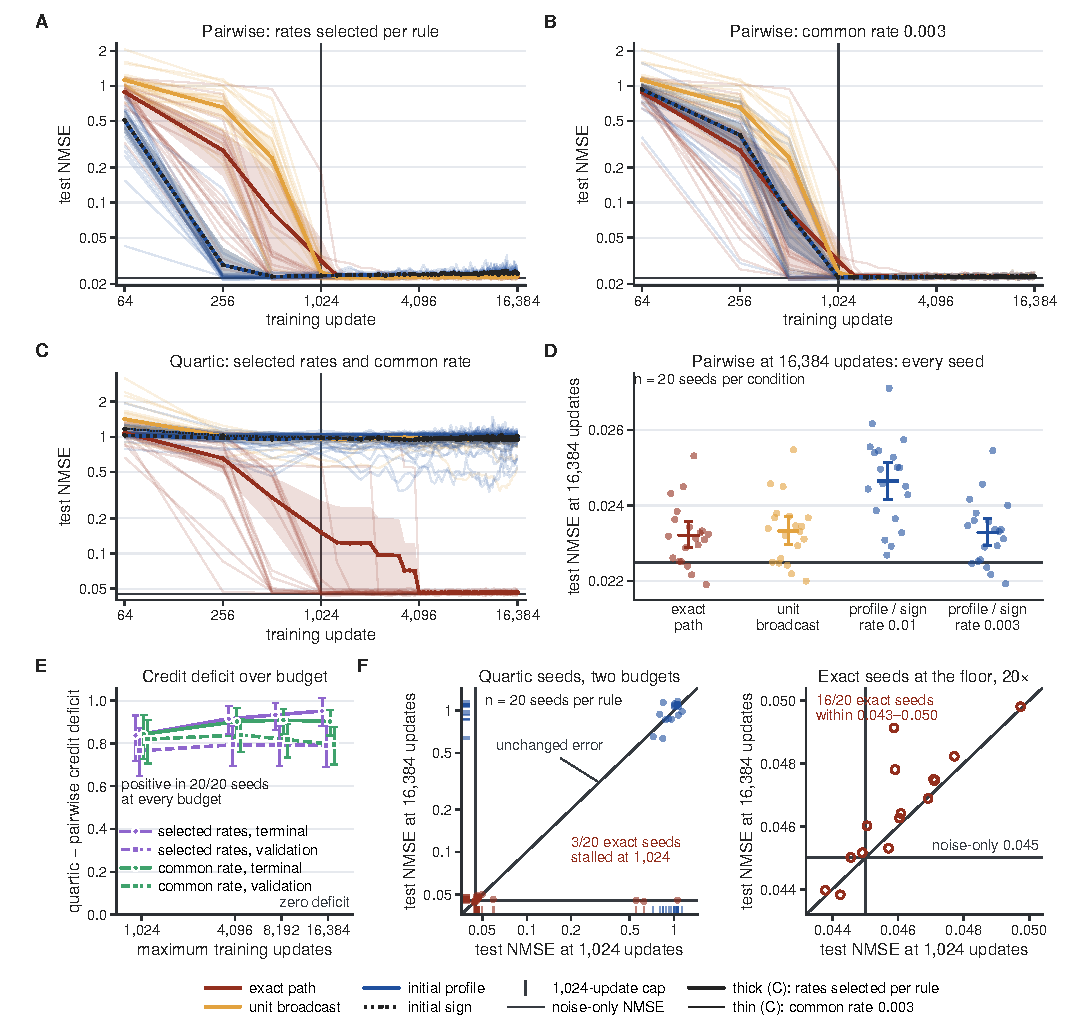
\includegraphics[width=\textwidth]{supplementary/curated/fixed_profile_budget.pdf}
\caption{\textbf{Longer matched budgets retain the task-dependent fixed-profile deficit.} \textbf{A,B}, Pairwise targets under Adam at the rates selected per rule (0.003 for exact path and unit broadcast, 0.01 for initial profile and initial sign) and at the common rate 0.003. In \textbf{A--D} and \textbf{F} colour names the credit rule (key below the sheet): dark red, exact path; amber, unit broadcast; blue, initial profile; black dotted, initial sign. Both axes of \textbf{A--C} are logarithmic; thick curves are means with a dot at each of the 64 measured checkpoints, tinted bands descriptive 95\% whole-seed bootstrap intervals, faint hairlines the twenty seed trajectories of each rule (no separate initial-sign fan: it coincides with the initial-profile fan where the rules share a rate); thin solid grey rules mark the 1,024-update cap (vertical) and the noise-only NMSE (horizontal; 0.0225 pairwise, 0.045 quartic). \textbf{C}, Quartic targets under both rate choices: exact-path and unit-broadcast selected rates equal the common rate, so those curves are drawn once; initial profile and initial sign are thick at the selected rate (0.01) and thin at the common rate (0.003). \textbf{D}, Test NMSE at 16,384 updates for all twenty pairwise seeds (dots, $n=20$ per condition), the mean (short rule) and its 95\% whole-seed bootstrap interval (whisker) for exact path, unit broadcast and the coinciding initial-profile/initial-sign pair at rate 0.01 and at 0.003, against the 0.0225 floor (thin grey rule). \textbf{E}, Quartic-minus-pairwise difference in initial-profile-minus-exact NMSE at budgets 1,024, 4,096, 8,192 and 16,384: circles/solid, terminal states; squares/dashed, validation-selected states; here colour names the rate view: violet, rates selected per rule (the series of main Fig.~4F); green, the common rate 0.003. Whiskers, 95\% paired whole-seed bootstrap intervals, offset slightly at each budget; every difference is positive in 20/20 seeds; the thin grey rule marks zero deficit. \textbf{F}, All twenty exact-path and twenty initial-profile quartic seeds at 1,024 and 16,384 updates (left, logarithmic axes; dots with a rug tick per seed on each axis); the thin grey diagonal marks unchanged error and the thin grey guides the quartic noise-only NMSE 0.045. The three exact seeds stalled at 1,024 updates (0.55--1.06; main Fig.~4D) are at the floor by 16,384; the right-hand panel enlarges the 0.043--0.050 window twenty-fold, where the other sixteen exact seeds (open circles) lie on both axes.}
\label{fig:si_fixed_profile_budget}
\label{fig:supp_credit_rule_extension}
\end{figure}

\begin{figure}[p]
\centering
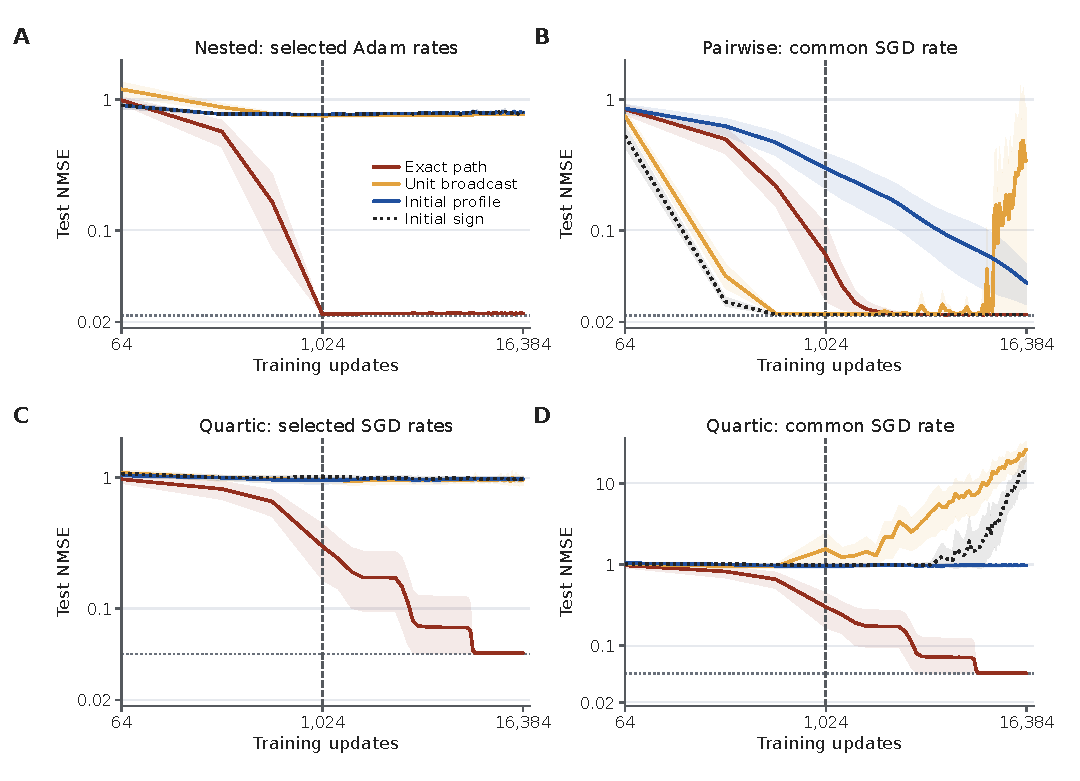
\includegraphics[width=\textwidth]{supplementary/curated/credit_optimizer_controls.pdf}
\caption{\textbf{Nested targets and SGD controls in the balanced budget extension.} \textbf{A}, The same condition as main Fig.~4E, repeated as the reference for the SGD panels: nested targets under Adam at the selected rates, 0.003 for exact-path and unit-broadcast credit and 0.01 for initial-profile and initial-sign credit. \textbf{B}, Pairwise targets under SGD at the common rate 0.03 for all four rules. \textbf{C,D}, Quartic targets under SGD at the selected rates (\textbf{C}: 0.03 for exact-path and initial-profile credit, 0.01 for unit and initial-sign broadcast) and at the common rate 0.03 (\textbf{D}); exact-path and initial-profile credit use rate 0.03 in both, so those runs are drawn once, in \textbf{C}, and \textbf{D} shows only the unit and initial-sign broadcast arms. Colours follow the main figures and line style also names the rule: exact path dark red solid, unit broadcast amber dashed, initial-profile broadcast (the calibrated broadcast of main Fig.~4) blue solid and initial-sign broadcast black dotted. Heavy curves show mean test NMSE from update 64 onward over the 64 saved checkpoints, thin lines are the 20 individual seeds of each rule, and pale bands give descriptive 95\% whole-seed bootstrap intervals of the mean (10,000 draws). A mean can sit where no seed does: in \textbf{B} the unit-broadcast mean rises to 0.34 at 16,384 updates because 2 of 20 seeds diverge (to 2.3 and 4.2) while 18 end at the floor, and 5 of 20 initial-profile seeds end at 0.050--0.125; in \textbf{D}, 18 of 20 unit-broadcast and 15 of 20 initial-sign seeds exceed NMSE 1. In \textbf{A} the three broadcast controls coincide to within 6\% after 1,024 updates, and in \textbf{C} all three stay between 0.94 and 1.09 without diverging, so their curves overprint and are told apart by line style. Vertical dashed lines mark the original 1,024-update cap; light grey solid rules mark the noise-only NMSE, printed under the left end of each rule (0.0225 in \textbf{A},\textbf{B}; 0.045 in \textbf{C}); \textbf{D} lies entirely above its floor of 0.045. In \textbf{B} the initial-sign and unit-broadcast means reach the floor by update 512 and the exact-path mean by 2,304, overprinting on it thereafter apart from the unit-broadcast excursions after 9,472 updates (2 of 20 seeds). \textbf{A} and \textbf{B} are single conditions, not a matched pair; only \textbf{C} and \textbf{D} contrast the two rate views at fixed task and optimizer. The update axis is logarithmic in every panel, and each vertical axis is logarithmic and tight to its own panel's seeds: 0.014--2.6 in \textbf{A}, 0.014--9.4 in \textbf{B}, 0.032--2.6 in \textbf{C} and 0.28--95 in \textbf{D}, which retains every divergent broadcast seed (up to 74).}
\label{fig:si_credit_optimizer_controls}
\label{fig:supp_credit_rule_extension_controls}
\end{figure}

\clearpage

% Curated from paper commit 7ee9157; original equations and protocol identities retained.
\section{Credit delivery in conductance-tree learning}
\label{note:conductance_learning}

\subsection{Conductance-tree tasks with aligned or opposed feature tuning}
\label{sec:conductance-credit-demand}
We tested whether context-dependent branch selection can create a learning advantage for spatially resolved credit in a conductance tree. The model contains four terminal compartments, two proximal compartments and a soma. It uses DendriNet's directed steady-state excitatory/inhibitory balance with identity reactivation; it is not a reciprocal cable model. All 24 positive conductances are trainable, including inhibitory gains and daughter and somatic couplings.

For each example, two independent latent variables $z_1,z_2\sim\mathcal U[-2,2]$ generate positive features $x_j^+=\exp(z_j)$ and $x_j^-=\exp(-z_j)$. Both subtrees receive the same latent features: terminals 0 and 2 receive $z_1$, and terminals 1 and 3 receive $z_2$. Each terminal has two excitatory and two inhibitory conductances. Its effective excitatory and inhibitory conductances and voltage are
\begin{equation}
 E_j=g_{E+,j}x_j^++g_{E-,j}x_j^- ,\qquad
 I_j=g_{I+,j}x_j^++g_{I-,j}x_j^- ,\qquad
 v_j=\frac{E_j}{1+E_j+I_j}.
\end{equation}
This normalization sets leak conductance to 1 and excitatory, inhibitory and leak reversal potentials to 1, 0 and 0. An independent binary context $c$ is sampled with equal probability. Proximal compartment $p\in\{0,1\}$ receives inhibitory activity $a_p=A\mathbf 1[c\ne p]$, with $A=10$ for the primary task pair. Its voltage and the somatic voltage are
\begin{equation}
 u_p=\frac{\sum_{j\in\mathrm{ch}(p)}g_{pj}v_j}
 {1+\sum_{j\in\mathrm{ch}(p)}g_{pj}+g_{I,p}a_p},\qquad
 v_s=\frac{g_{s0}u_0+g_{s1}u_1}{1+g_{s0}+g_{s1}},
\end{equation}
where $\mathrm{ch}(p)$ denotes the two terminal daughters of proximal compartment $p$. Here $u_p=v_{4+p}$ denotes a proximal voltage; thus $v_j$, $j=0,\ldots,5$, indexes all six nonsomatic compartment voltages. All conductances are parameterized by their logarithms.

Labels are the noiseless somatic responses of a teacher with this exact model, establishing a constructive zero forward-error floor. In the aligned task every teacher terminal has nominal gains $(8,0.25,0.25,8)$, ordered as $(E+,E-,I+,I-)$. In the opposed task terminals 2 and 3 instead have $(0.25,8,8,0.25)$. Teacher log gains receive independent Gaussian perturbations of standard deviation 0.15, shared across the paired tasks. Parent inhibitory gains are nominally 15, daughter couplings are $(20,0.2)$ in each subtree, and somatic gains are 4. Students start with terminal gains 1 and these same other nominal gains, with independent Gaussian perturbations of standard deviation 0.4 applied to all 24 log gains. No exact symmetry is imposed. Paired tasks have identical student initializations, input samples, contexts and minibatches; their teacher tuning differs. Identical input samples do not imply identical task input-sensitivity spectra.

Training minimizes half the mean squared error divided by training-target variance. Writing $\delta=(v_s-y)/\operatorname{Var}_{\mathrm{train}}(y)$, the exact update uses the path factor $q_j=\partial v_s/\partial v_j$ and local eligibility $\partial v_j/\partial\theta_j$. Here $\theta_j$ is a local log conductance. Excitatory eligibilities retain the factor $(1-v_j)/D_j$, inhibitory eligibilities retain $-v_j/D_j$, and daughter-coupling eligibilities retain $(v_{\mathrm{child}}-v_{\mathrm{parent}})/D_{\mathrm{parent}}$, together with their corresponding input and conductance factors; $D$ is the local conductance denominator. Thus changing the credit rule leaves all local voltage derivatives intact. Somatic couplings receive the exact somatic factor 1 under every rule.

The six non-somatic path factors are delivered exactly, replaced by 1, replaced by a fixed initial profile, or projected into three fixed spatial patterns. The initial profile is the mean initial exact path field on 512 independently generated, unlabeled calibration examples. The three-pattern dictionary retains this profile on terminals $(0,1)$, terminals $(2,3)$ and proximal compartments $(4,5)$, respectively, with zero entries elsewhere. If $A$ is the resulting six-by-three matrix, the oracle rule delivers $A(A^\top A)^{-1}A^\top\boldsymbol q$ for the current example. Its coefficients use the current exact field. It tests a restricted spatial dictionary with an oracle encoder; it is not a locally estimated routing rule or evidence that three independent external errors are necessary. At fixed parameters the binary context generates at most two path profiles, so this experiment concerns branch selection rather than a six-dimensional or quartic-interaction requirement.

Each task/seed has 2,048 training, 1,024 validation, 4,096 test and 1,024 diagnostic examples, independent of the calibration sample and of one another. No noise is added to labels. Across the 20 fresh teachers, mean test-target variance is 0.024108 for aligned tuning and 0.014691 for opposed tuning. Test NMSE divides mean squared error by each test set's clean target variance.

Development comprised three seeds, four regimes, four credit rules, two optimizers and three rates, for 288 fits. Every outcome is retained. The regimes were aligned strong gating, opposed strong gating, opposed moderate gating ($A=1$), and opposed ungated ($A=0$). Before development outcomes, the primary strong-opposed regime had to satisfy mean teacher rank-one path capture at most 0.90 and mean exact-Adam validation NMSE at most 0.02, with a declared fallback order. Selection did not use the between-rule gap. Strong opposed tuning qualified, and a separate selection freeze preceded the 20 fresh paired blocks. Adam rates were $0.003,0.01,0.03$, and SGD rates were $0.03,0.1,0.3$. Each task/rule/optimizer selected the rate with lowest mean development best-validation NMSE; a common rate minimized the mean over rules. In the fresh task pair all selected rates equal their common rates: 0.03 for Adam and 0.3 for SGD. The common-rate results therefore reuse the same fits. The fresh cohort comprises $20\times2\times4\times2=320$ fits.

Minibatches contain 128 examples sampled with replacement. Adam uses $\beta_1=0.9$, $\beta_2=0.999$ and $\epsilon=10^{-8}$; SGD has no momentum. The original budget is 4,096 updates, with global gradient norm capped at 10 and log conductances projected into $[-7,7]$. Validation checkpoints are updates 0, 64, 256, 1,024, 2,048 and 4,096; the lowest-validation-loss checkpoint supplies the primary test endpoint. Every fresh fit continues, with its original optimizer and minibatch state, to 16,384 updates, adding validation checkpoints 8,192, 12,288 and 16,384. This extension was declared before fresh outcomes and retains earlier checkpoints when selecting its endpoint. These are fixed optimization budgets, not claims of convergence. No fresh or extended fit undergoes gradient-norm clipping. Exact and oracle fits never reach a parameter bound, whereas broadcast fits can do so.

The primary interaction is the calibrated-minus-exact NMSE gap for opposed tuning minus the corresponding gap for aligned tuning. Confidence intervals are paired percentile bootstrap intervals from 20,000 resamples of the 20 teacher/initialization seed blocks. Full rule-specific, seed-specific and checkpoint-specific outcomes are supplied. Post-fit diagnostics report squared-energy capture for the path field and the loss-weighted field, their best rank-one projections, and projection into the frozen initial profile after weighting by squared local eligibility, with or without squared somatic error. All are oracle diagnostics rather than additional training rules.

To identify cancellation across contexts, each rule is evaluated at the same initial, 256-update, primary-best and extended-best states of each selected Adam fit. For a given state, the cancellation ratio is the norm of the probability-weighted sum of context-conditional distal gradients divided by the probability-weighted sum of their norms. Lower values indicate stronger cancellation. All 2,560 audited mean gradients reproduce the training adapter exactly. Since path factors and fixed profiles are positive, per-example approximate gradient estimates have nonnegative inner products with exact per-example gradients; the failure being tested concerns averaging conflicting examples.

A separately timestamped posthoc sensitivity restarts every fresh condition from its original initialization for 16,384 updates with wider log bounds $[-20,20]$ and unchanged rates. It also replays every original-bound trajectory to record first contact with each parameter bound. These 640 trajectories reuse the same 20 seed blocks. All 320 original-bound replays reproduce every final parameter exactly. The wider-bound interaction remains positive in all 20 seeds for both optimizers. At the last saved checkpoint before each calibrated Adam fit's first original bound contact, its opposed-task gap is already positive in all 20 seeds. Some broadcast parameters also reach the wider bounds, so this control establishes robustness across a much wider conductance range rather than unbounded convergence. The retained moderate-gating development regime also shows a substantial broadcast deficit despite teacher rank-one path capture near 0.98. Raw path-energy capture is therefore not a sufficient criterion for learning: a small spatial component can distinguish the gradient contributions of competing contexts.

\subsection{Local inhibitory gating in the conductance task}
\label{sec:local_conductance_gate}
\label{sec:review_followups}
This study was specified after exposure to a referee panel's exploratory gate results. Those runs are excluded here. The protocol and numerical adapter were committed before execution on twenty new seed blocks, 2026090801--2026090820. Within each seed, aligned and opposed targets and all nine rules shared teacher perturbations, initial students, features, contexts and minibatch streams. The 24-conductance model, nominal gains, input streams and independent perturbations are defined in Section~\ref{sec:conductance-credit-demand}; every conductance remains plastic.

Let $\delta=(V_s-y)/\operatorname{Var}_{\rm train}(y)$ denote the somatic error and $a_p\in\{0,10\}$ the inhibitory activity at parent $p$. The hard local rule multiplies terminal eligibilities by $\delta\bm1[a_p=0]$, while proximal and somatic eligibilities receive $\delta$. It uses neither exact paths nor exact-field projections during learning. A secondary continuous gate uses $\delta/(1+g_p^{\rm I}a_p)$ at terminals, again retaining unit proximal and somatic multipliers. Both receive an imposed inhibitory context and an output error; neither generates those signals autonomously.

Exact, uniform, calibrated and three-profile oracle rules retain the previous comparators. Calibration averages initial exact path derivatives on 512 unlabeled examples. Two weighted leaf-subtree profiles with oracle projection amplitudes and unit proximal credit test the context distinction separately from proximal provision. The earlier three-profile oracle also includes a weighted proximal-pair column. The new control therefore has two distal profiles plus a fixed proximal rule, rather than an entirely two-dimensional six-site dictionary. Further controls reverse the distal gate or apply it at the proximal compartments as well. In the latter, inhibitory eligibility is nonzero only when inhibition is present, while its credit multiplier is then zero; both proximal inhibitory gradients vanish identically.

Data sizes, half-NMSE objective, Adam parameters, batch size 128, clipping threshold ten and log bounds $[-7,7]$ were unchanged. The primary rate was 0.03; 0.01 and 0.1 were symmetric robustness conditions for all rules. All $20\times2\times9\times3=1,080$ trajectories continued to 16,384 updates. Minimum validation NMSE selected a state within the primary 4,096-update and extended windows, while fixed endpoints and every saved observation remain available separately.

Two prespecified paired contrasts used exact two-sided sign-flip tests: opposed-task broadcast-minus-local-gate NMSE, and the difference in this gap between opposed and aligned tasks. Both were positive in all twenty seeds, with Holm-adjusted $P=3.81\times10^{-6}$ in the two-test family. Intervals use 20,000 whole-seed bootstrap draws. Other rates, budgets and contrasts are descriptive. The local-minus-exact opposed-task difference was $1.49\times10^{-6}$ (95\% interval, $-1.60\times10^{-6}$ to $4.86\times10^{-6}$), and the maximum local-gate seed error was $5.47\times10^{-5}$. These satisfy the frozen practical precision reference without establishing asymptotic equivalence.

At the primary rate, exact, proper local gates and both oracle dictionaries contacted no bounds; opposed broadcast contacted bounds in 18/20 fits by 4,096 and 20/20 by 16,384. No fit clipped gradients. Ten mechanism tests verify the derivatives, absence of exact-path access in the hard local update, and the proximal eligibility failure. Excluded historical-seed replays reproduced prior exact, unit and calibrated trajectories bit for bit and the independently projected dictionary to floating-point association error. Protocols, fresh-seed outcomes, states, curves and validation records are in \texttt{source\_data/conductance\_local\_gate/}.

\paragraph{Retained first conductance study.}
A separately frozen first study used the same seven-compartment topology but one excitatory and one inhibitory feature per terminal, giving 16 trainable conductances. An independent context selected one subtree. Its two terminal latent inputs were $z_1,z_2\sim\mathcal U[-2,2]$; the inactive subtree received $-\rho z_j+\sqrt{1-\rho^2}u_j$, where $u_j$ were independent draws from the same distribution and $\rho\in\{0,1\}$ set independent or opposite distractors. Each terminal received $\exp(z)$ through its excitatory contact and $\exp(-z)$ through its inhibitory contact, with the corresponding selected or inactive latent value. The four development regimes were ungated/independent, strong-gated/independent, strong-gated/opposite and moderate-gated/opposite, using inhibitory activities $A=0,10,10,1$, respectively. Nominal teacher excitatory gains were $(0.25,8,0.25,8)$ and inhibitory gains $(8,0.25,8,0.25)$; nominal student gains were 2 and 0.7, respectively. Parent inhibition, daughter couplings and somatic gains were 15, $(20,0.2)$ per subtree and 4, as above. Teacher and student log gains had independent Gaussian perturbations of standard deviations 0.15 and 0.4. Labels were noiseless outputs of the same teacher circuit. Dataset sizes, calibration, optimizers, learning-rate grids, batch size, validation cadence and the two update budgets matched those specified above. Three development seeds, four regimes, three rules, two optimizers and three rates gave 216 development fits. The declared teacher-geometry and exact-learnability criteria selected strong-gated/opposite inputs, paired with the ungated/independent control; this comparison changes both gating and distractor dependence. Twenty fresh seeds gave 240 fits, all continued to the larger budget. All outcomes are retained. After 16,384 updates, its gated-task calibrated-minus-exact gap was $0.000502$ [$0.000267$, $0.000772$] NMSE, positive in all 20 seeds; under Adam the mean broadcast error remained below 0.0006 NMSE. This small precision effect motivated the separately declared opponent-tuning model above. The first result and all unsuccessful development regimes remain part of the evidence.
\paragraph{Expanded learning-rate screen.}
Because the original development selection lay at the upper edge of its rate grid, we performed a separately specified post hoc screen using the original three development seeds (201--203). Each of the four credit rules received the same six-rate search on both the aligned and opposed tasks: $\{0.003,0.01,0.03,0.1,0.3,1\}$ for Adam and $\{0.03,0.1,0.3,1,3,10\}$ for SGD. We reran the original rates alongside the added rates, giving every fit 16,384 updates and selecting its minimum validation NMSE among checkpoints at 0, 64, 256, 1,024, 2,048, 4,096, 8,192, 12,288 and 16,384 updates. All other task, initialization, optimizer and conductance-bound settings remained those of the original opponent study. The screen comprises 288 retained fits; no test outcome entered rate selection.

Before inspecting these outcomes, we specified that an improvement of at least 0.01 NMSE and at least 10\% in mean opposed-task validation error for either broadcast rule would trigger a follow-up on the 20 previously used fresh seed blocks. The first criterion compared the best added rate with the best original-grid rate at the same update budget; a pre-outcome addendum also compared the best rate across the whole grid with the originally selected rate (0.03 for Adam and 0.3 for SGD). Any triggered follow-up would retune all four rules on both tasks using development validation alone and would be reported as reuse of existing blocks. Neither criterion was met. No added rate improved the opposed-task broadcast minimum; within the original grid, reducing Adam's rate to 0.003 lowered mean validation NMSE by approximately 0.00647 (0.89\%), and reducing the unit-broadcast SGD rate to 0.1 lowered it by 0.03348 (4.46\%). Calibrated-broadcast SGD retained rate 0.3. We therefore performed no additional fresh-block fits. These results address a finite grid at the stated update budget and do not establish optimizer-independent convergence.

\subsection{Input grouping and restricted credit in directed conductance trees}
\label{sec:conductance_grouping_bridge}

We used a minimal directed shunting model to test input grouping while holding the branching shape and parameter counts fixed. Four terminal compartments fed two proximal compartments and a soma. Every model had seven compartments, six child couplings, four excitatory contacts, six inhibitory contacts and sixteen trainable conductances. Leak conductance was one; excitatory and inhibitory reversal potentials were one and zero. All compartment activations were the identity, and the soma had no direct synaptic inputs or additional decoder. Let $i\in\{0,1,2,3\}$ index terminal compartments and $j\in\{1,2\}$ proximal compartments. Write $T_i$, $P_j$ and $S$ for terminal, proximal and somatic voltages. The pair $\mathcal S_j$ contains the terminals assigned to proximal compartment $j$. Terminal $i$ has synaptic conductances $g_i^{\mathrm E}$ and $g_i^{\mathrm I}$, and $b_{ji}$ couples it to proximal compartment $j$. The maximal proximal shunt conductance is $h_j$, and $a_j$ couples that compartment to the soma. For terminal activities $x_i^{\mathrm E},x_i^{\mathrm I}$ and proximal shunt input $z_j$,
\begin{align}
T_i&=\frac{g_i^{\mathrm E}x_i^{\mathrm E}}
 {1+g_i^{\mathrm E}x_i^{\mathrm E}+g_i^{\mathrm I}x_i^{\mathrm I}},\\
P_j&=\frac{\sum_{i\in\mathcal S_j}b_{ji}T_i}
 {1+\sum_{i\in\mathcal S_j}b_{ji}+h_jz_j},\\
S&=\frac{a_1P_1+a_2P_2}{1+a_1+a_2}.
\end{align}
The positive local input $z_j$ controls shunt conductance; it carries no teaching signal. Conductances were parameterized as $g=\exp(\theta)$, with $\theta\in[-5,5]$. The matched resources were compartment, contact, coupling and parameter counts and the admissible conductance range; total learned conductance was not constrained to be equal. No fresh run reached a parameter bound. The NumPy implementation was checked compartment by compartment against the repository's production \texttt{forward\_branch\_dynamics} function in its identity-activation, zero-numerical-offset configuration. All sixteen log-conductance derivatives and ten input derivatives agreed with autograd to the numerical tolerances reported in the accompanying tests. This is a directed steady-state model, not a reciprocal cable or spiking model.

The three groupings were $(01\mid23)$, $(02\mid13)$ and $(03\mid12)$. A planted teacher used the same conductance equations, with independent Gaussian perturbations of standard deviation $0.25$ in log conductance around $g^{\mathrm E}=2$, $g^{\mathrm I}=0.7$, $h=3$, $b=3$ and $a=4$. Independent student perturbations had standard deviation $0.4$ around these centers and were shared across paired candidate groupings, credit rules and optimizer settings. Student initialization did not use teacher coefficients. Teacher tasks permuted terminal excitatory/inhibitory input pairs together; the proximal inputs retained their identities. Paired task inputs were inversely permuted so that the realized target values were identical across the three tasks. Thus each task had the same input distribution and the same spectrum of the input-gradient second moment. The latter was verified from 2,048 paired probes per seed; its matrix entries could differ by the corresponding coordinate permutation. Compatibility meant that the student's input grouping matched the teacher's grouping. These tasks are planted mechanistic positive controls within one model class, rather than tests of transfer to an unseen class of biological computations.

Each input was $\exp(\sigma Z-\sigma^2/2)$ for independent standard-normal $Z$. We used $\sigma=0.7$ for terminal excitatory and inhibitory inputs and $\sigma=1.2$ for proximal shunt inputs. All activities and conductances were strictly positive, all voltages lay between the reversal potentials, and there was no label noise. Each task used 1,024 training, 1,024 validation, 4,096 test and 256 calibration examples from independent random streams. Within a task, every candidate and credit rule received the same examples and minibatch indices. Training minimized half-MSE divided by the training target variance. Reported NMSE is MSE divided by the target variance of the evaluation split; it is dimensionless and is not a percentage.

Four feedback conditions shared the forward model. Let $V_n$ be the voltage of compartment $n$ and $L$ the training loss. Write $\rho_n=\partial S/\partial V_n$ for its current exact path sensitivity and $\delta_0=\partial L/\partial S$ for the somatic loss derivative. Exact transport supplied $\delta_0\rho_n$. A fixed calibrated broadcast supplied $\delta_0\gamma_n$, where $\gamma_n$ was the mean initial path sensitivity of that student's own forward states on the label-free calibration inputs. The profile was frozen during training. A one-profile projection used the same $\bm\gamma$ and supplied its best Euclidean fit to the current nonsomatic field. The two-subtree condition restricted $\bm\gamma$ to each proximal compartment and its two terminal descendants, giving disjoint columns $\bm A_j$. Its coefficients were
\begin{equation}
c_j=\frac{\bm A_j^{\mathsf T}\bm\rho}
 {\bm A_j^{\mathsf T}\bm A_j}.
\end{equation}
The one-profile projection used the analogous coefficient with $\bm A=\bm\gamma$. These per-trial coefficients had access to the current exact student path field; both projection rules are oracle diagnostics of restricted feedback, not learned coefficient estimators. Soma error remained exact in every condition. Each conductance update multiplied the delivered compartment error by its local conductance eligibility, including the chain derivative of the exponential parameterization. For a child coupling, the local conductance derivative was $(V_{\rm child}-V_{\rm parent})/G_{\rm parent}^{\rm tot}$, where $G_{\rm parent}^{\rm tot}$ is the parent's total open conductance. Credit geometry was evaluated at the corresponding exact-learning model's common checkpoint state; the reported path-capture normalization excluded the soma.

We used 1,000 minibatch updates of size 128, with checkpoints at 0, 10, 100, 300 and 1,000. Stochastic gradient descent (SGD) and Adam were evaluated separately; Adam used $(\beta_1,\beta_2)=(0.9,0.999)$ and $\epsilon=10^{-8}$. One learning rate per optimizer was chosen by averaging final validation NMSE over five development seeds (15300--15304), all task/student groupings and all four credit rules. The original SGD grid was $0.001,0.003,0.01$; because its optimum was at the upper boundary, an additional development-only bracket tested $0.03,0.1,0.3,1$. Every result, including unstable high-rate trajectories, was retained. Adam tested $0.003,0.01,0.03$. The selected rates were $0.3$ for SGD and $0.01$ for Adam. These settings were frozen before the twenty fresh seeds (15400--15419), producing $20\times3\times3\times4\times2=1,440$ fits and 7,200 checkpoint outcomes. No learning rate, horizon or credit rule was selected using fresh training outcomes. The two primary contrasts were the Adam exact-gradient grouping effect and the Adam calibrated-broadcast-minus-exact effect within compatible groupings. Other contrasts are descriptive optimizer and feedback-resolution sensitivities.

Inference used the seed as the independent unit. Each seed's compatible mean averaged its three teacher-task permutations; its incompatible mean additionally averaged the two mismatched student groupings per task. Confidence intervals used 10,000 bootstrap resamples of these paired seed summaries. Intervals are pointwise rather than simultaneous across all reported subgroup comparisons. All sources, rates, states, physical-domain checks and numerical tests are retained under \texttt{source\_data/morphology\_conductance}; execution code is under \texttt{scripts/morphology\_conductance}.

\paragraph{An interaction lower bound for this conductance model.}
Let $R_i$ denote a teacher terminal response, $A_j=(1+\sum_i b_{ji}+h_jz_j)^{-1}$ its proximal attenuation, and $\beta_j=a_j/(1+a_1+a_2)$. The sum in $A_j$ runs over the teacher terminals assigned to proximal compartment $j$. The teacher output is a sum of terms $\beta_j b_{ji}R_iA_j$. Let $p_{\rm teacher}(i)$ and $p_{\rm student}(i)$ denote the proximal parent assigned to terminal $i$ in the teacher and student, respectively, and write $p(i)=p_{\rm teacher}(i)$. For terminal $i$, set $j=p(i)$. Because terminal inputs and proximal shunt inputs are independent, a term whose terminal and teacher shunt belong to different \emph{student} proximal input blocks has the centered interaction
\begin{equation}
H_i=\beta_jb_{ji}(R_i-\mathbb E R_i)(A_j-\mathbb E A_j).
\end{equation}
Every admissible student output is additive across its two proximal input blocks. Each such $H_i$ is orthogonal to all functions additive across those blocks, and the omitted $H_i$ are mutually orthogonal. Therefore, for every choice of the student's conductances,
\begin{equation}
\mathbb E[(S_{\rm teacher}-S_{\rm student})^2]
\geq\sum_{i:\,p_{\rm student}(i)\ne p_{\rm teacher}(i)}
 (\beta_{p(i)}b_{p(i)i})^2
 \operatorname{Var}(R_i)\operatorname{Var}(A_{p(i)}).
\end{equation}
The bound is zero for compatible groupings. It is a lower bound for the larger class of arbitrary functions additive across the student's proximal blocks, not a claim that the constrained rational student attains it. Its validity relies on the specified independent inputs, identity somatic activation and absence of direct somatic synaptic inputs; it does not extend automatically to arbitrary conductance architectures or nonlinear readouts. An equivalent obstruction is the absence of a mixed derivative between a terminal input and a shunt input assigned to the other student subtree.

We specified this diagnostic before the fresh training outcomes and retained the learner and rate-selection procedure unchanged. Population lognormal moments were evaluated with 32-, 64- and 128-node Gauss--Hermite quadrature. The primary bound used 128 nodes; the maximum change from 64 to 128 nodes was below $8\times10^{-17}$ in normalized-MSE units. This is a converged numerical evaluation of an analytic bound, not a formally certified quadrature error. Across the fresh teacher draws, the mean incompatible population-NMSE lower bound was $0.013222$, with a minimum of $0.005367$ across task/candidate pairs. These are population lower bounds, distinct from held-out sample NMSE.

\subsection{Graded context and independently specified sensory targets}
\label{sec:gate_generalization}

The binary-context experiment above leaves two questions open: whether a local
gate works with continuously varying inhibition, and whether its benefit extends
to targets not generated by the conductance teacher. We retained the directed
seven-compartment circuit but supplied four independent latent features
$z_i\sim\mathcal U[-2,2]$, rather than duplicating two features across subtrees.
Each terminal received $\exp(z_i)$ and $\exp(-z_i)$ through its excitatory and
inhibitory contacts. Context $c$ supplied proximal inhibitory activities
$a_0=10c$ and $a_1=10(1-c)$. All rules trained the same 24 log conductances
and an affine readout $\widehat y=w_{\rm out}V_s+b_{\rm out}$, using its exact
somatic error and the same exact local conductance eligibilities.

Three tasks separated these changes. The \emph{graded teacher} task used
$c\sim\mathcal U[0,1]$ and noiseless outputs of the opposed-tuning conductance
teacher. It remains a model-matched task. Two other tasks defined targets
independently of that teacher:
\begin{equation}
t_0(\bm z)=\frac{\tanh z_1+\tanh z_2}{2},\qquad
t_1(\bm z)=-\frac{\tanh z_3+\tanh z_4}{2},\qquad
y=(1-c)t_0(\bm z)+ct_1(\bm z).
\end{equation}
In \emph{sensory selection}, a balanced binary context selects one stream;
in \emph{graded sensory mixture}, uniform continuous context weights both.
These are steady-state analogues of context-dependent selection, not a
reproduction of temporal evidence accumulation or of a particular cortical
circuit. The externally specified targets are not guaranteed representable by
this neuron.

Exact paths and unit broadcast were compared with three distal delivery rules.
The original proportional gate used $\gamma_p=1/(1+g_p^{\rm I}a_p)$.
A relative-resistance gate instead used
\begin{equation}
\gamma_p^{R}=\frac{D_p^{\rm base}}{D_p^{\rm base}+g_p^{\rm I}a_p},\qquad
D_p^{\rm base}=1+\sum_{i\in\operatorname{children}(p)}g_{i\to p}^{\rm den}.
\end{equation}
This equals the parent's input resistance divided by its uninhibited value.
Both gates use parent-compartment state, broadcast to its two terminals;
they do not evaluate exact paths or project an exact error field.
Proximal and somatic multipliers remain one. A swapped proportional gate
uses the other parent's inhibitory activity, testing misassignment with the
same available signals rather than supplying a local mechanism.

The relative-resistance rule has a specific relationship to exact credit in
this directed, identity-output circuit. For a terminal $i$ with parent $p$,
\begin{equation}
\frac{\partial V_s}{\partial V_i}
=\frac{g_{p\to s}^{\rm den}g_{i\to p}^{\rm den}}
 {D_sD_p^{\rm base}}\,\gamma_p^{R}.
\end{equation}
Here $D_s=1+\sum_pg_{p\to s}^{\rm den}$. At fixed weights, the prefactor is
independent of the example, while $\gamma_p^R$ preserves the context dependence.
This identity motivates the rule but does not guarantee the same training
trajectory: prefactors differ across parameters and change as conductances
learn. Nor does it extend unchanged to reciprocal cables or active branches.

Three development seeds compared five rules at Adam rates 0.01, 0.03 and 0.1.
For each task and rule, the minimum mean development-validation error selected
one rate before twenty fresh paired seeds were run. This was an internally
frozen follow-up after development, not an externally preregistered study.
All three rates were retained in the fresh cohort, giving 900 trajectories;
primary summaries use only the fixed development-selected rate. Each trajectory
used 2,048 training, 1,024 validation and 4,096 test examples, minibatches of
128 and 4,096 updates. Validation was evaluated every 64 updates and selected
the state; test outcomes selected neither states nor rates. NMSE divides by
the target variance in each evaluation split. Log conductances remained in
$[-7,7]$; readout weights were unconstrained, and gradient norms were clipped
at 10. The readout started with slope one for the graded teacher and four for
the external targets, with a common bias centering training targets within
each paired seed. Initial conductances and minibatch streams were paired
across rules. Intervals are descriptive 95\% whole-seed percentile bootstrap
intervals; they do not establish equivalence to exact credit.

Numerical derivatives checked all 26 trainable parameters. A separate check
against DendriNet's production branch dynamics reproduced the circuit's
voltages and exact conductance gradients. Sentinel tests prohibit exact-path
evaluation by the local rules. These validate the independent adapter, not a
population-level or reconstructed-neuron implementation.

Table~\ref{tab:gate_generalization} reports the fresh-seed outcomes. Relative
resistance gating reduced NMSE relative to unit broadcast in all twenty seeds
for each task. The paired mean reductions were $0.00242$
[$0.00147$, $0.00362$] for the graded teacher, $0.000157$
[$0.000141$, $0.000173$] for sensory selection, and $0.00776$
[$0.00655$, $0.00903$] for graded mixtures. In sensory selection both exact
credit and local gating already gave small absolute errors; the advantage
over broadcast is a precision improvement, not rescue from task failure.
The original proportional gate also learned the graded teacher and binary
sensory selection accurately, but gave higher mean graded-mixture error than
unit broadcast ($0.123$ versus $0.106$). Relative resistance gating gave
$0.09786$, close in magnitude to exact credit's $0.09783$, but with a small
positive paired difference of $2.70\times10^{-5}$
[$1.24\times10^{-5}$, $4.20\times10^{-5}$]. Similar means are therefore not
evidence of mathematical or statistical equivalence. Wrong-branch gating
performed poorly on all three tasks.

The outcomes remain conditional on the optimizer, bounded conductances and
training window. For the graded teacher, 13/20 broadcast trajectories and no
exact or local-gate trajectories contacted a bound. For sensory selection,
the counts were 20/20 for broadcast, 3/20 for exact, 4/20 for the proportional
gate and 5/20 for relative resistance gating. For graded mixtures, 19/20
exact and 20/20 proportional-gate trajectories contacted bounds, compared
with none for broadcast or relative resistance gating. These counts concern
the full fixed-rate trajectory, not necessarily its validation-selected state.
The appreciable residual with exact credit in graded mixtures prevents
attributing all error to restricted feedback: representational and
optimization limitations remain unresolved. No claim of asymptotic optimality,
necessity of dendritic anatomy, or learning in reconstructed or spiking neurons
follows from this cohort.

The three development seeds were 2026091700--2026091702, and fresh seeds were
2026091800--2026091819. Compact endpoints, means, paired contrasts and the
protocol/source hashes are retained under
\path{source_data/curated_publication/gate_generalization_*}; the generator,
rate-selection protocol and replay checks are in
\path{scripts/conductance_gate_generalization/}. Re-evaluating every archived
validation-selected parameter state reproduced all 900 reported test NMSEs.

\subsection{Sensory selection in DendriNet populations}
\label{sec:dendrinet_selection}

The independent seven-compartment implementation isolates the gate mechanism.
To test its transfer to the production network implementation, we trained
DendriNet populations with fixed, grouped input contacts. The principal
configuration contained sixteen somata, each with a $[4,2]$ tree: eight
terminal compartments, four proximal compartments and one soma. Each pair
of terminals received two features of one sensory stream. An affine readout
combined the sixteen somatic voltages. Leak and reversal potentials were
those of the artificial conductance models in Methods. All excitatory,
inhibitory and coupling conductances, and the readout, were plastic; input
supports were fixed rather than chosen by adaptive contact selection.

\paragraph{Tasks and forward controls.}
For four streams indexed by $b=0,1,2,3$, independent latent features
$z_{bj}\sim\mathcal U[-2,2]$, $j=1,2$, supplied positive terminal inputs
$\exp(z_{bj})$ and $\exp(-z_{bj})$. A one-hot cue $\bm c$ selected one stream.
Every terminal also received the same four excitatory cue channels, so none
of the forward controls lacked context information. The targets were
specified independently of the network:
\begin{equation}
y=\sum_{b=0}^3 c_b(-1)^b
\left[\frac{\tanh z_{b1}+\tanh z_{b2}}2
       +\beta\tanh z_{b1}\tanh z_{b2}\right].
\label{eq:si_selection_target}
\end{equation}
Alternating signs prescribe opposed feature tuning across streams. They do
not supply targets to the network. The primary task sets $\beta=0$ and uses
identity compartment outputs. A secondary condition sets $\beta=0.25$ and
uses $\tanh(V_p)$ at proximal compartments, allowing the two features to
interact. This secondary condition changes both target and representation;
it is not an isolated test of the effect of adding a nonlinearity.

In the shunting forward model, proximal inhibitory activity was
$a_b^{\rm I}=4(1-c_b)$. With $D_p^0=1+\sum_i g_{i\to p}^{\rm den}$ and child current
$I_p=\sum_i g_{i\to p}^{\rm den}a_i$, the proximal voltage was
$V_p^{\rm sh}=I_p/(D_p^0+g_p^{\rm I}a_b^{\rm I})$. Tonic inhibition replaced
$a_b^{\rm I}$ by its training-distribution mean $\bar a^{\rm I}=3$; the excitatory cue inputs
were unchanged. A current-injection control preserved that tonic denominator
but varied a context-dependent current:
\begin{equation}
V_p^{\rm cur}=
\frac{I_p-g_p^{\rm I}(a_b^{\rm I}-\bar a^{\rm I})\bar V_p}
     {D_p^0+g_p^{\rm I}\bar a^{\rm I}}.
\end{equation}
Here $\bar V_p$ was the mean tonic voltage at initialization, estimated
using training inputs and then held fixed. This matches the incremental
inhibitory current at that reference voltage, not the full voltage
distribution throughout training. Shunting, tonic and current models had
the same parameter count, cue channels and paired initial parameters.

\paragraph{Learning rules.}
The local rules detached intercompartment connections when differentiating
the loss, while retaining each compartment's exact local derivatives.
The affine readout supplied a separate somatic error to each neuron:
\begin{equation}
\widehat y=\sum_{u=1}^{16}w_u^{\rm out}V_u+b^{\rm out},\qquad
\ell=\frac{(\widehat y-y)^2}{2\operatorname{Var}_{\rm train}(y)},\qquad
\delta_u^V=\frac{w_u^{\rm out}(\widehat y-y)}{\operatorname{Var}_{\rm train}(y)}.
\end{equation}
Training averaged $\ell$ over the minibatch. Thus broadcast here means
sharing a neuron's error across its own compartments, not sharing one
scalar across all sixteen neurons.
Proximal and somatic updates used this error without spatial attenuation.
At a terminal whose proximal parent was $p$, the relative-resistance rule
instead delivered
\begin{equation}
\widehat\delta_{ui}^V=\delta_u^V h_{up},\qquad
h_{up}=\frac{D_{up}^0}{D_{up}^0+g_{up}^{\rm I}a_b^{\rm I}}.
\label{eq:si_dendrinet_gate}
\end{equation}
Unit broadcast set $h=1$. A wrong-branch control cyclically permuted
the four parent gates within each neuron. A uniform-gain control replaced
them by their within-neuron root-mean-square,
$h_u^{\rm rms}=(\sum_{p=1}^4h_{up}^2/4)^{1/2}$, preserving
the gate-vector norm but not the norm of the eligibility-weighted parameter
update. Exact BP provided a reference. All five rules shared the same
forward model within a condition and trained the same parameters.
In the tonic and current controls, the local gate still used the supplied
trial-dependent inhibitory cue. These conditions therefore test a proposed
credit signal without its corresponding forward shunt, not the exact
resistance of those alternative forward models. In the nonlinear-parent
condition the gate omitted the parent's activation derivative. Local
training accessed neither exact path products nor exact-gradient diagnostics.

The chain rule explains this distinction. In the shunting model, exact
terminal credit is
\begin{equation}
\delta_{ui}^V=\delta_u^V\,
\frac{g_{p\to u}^{\rm den}g_{i\to p}^{\rm den}}{D_uD_p^0}
h_{up} f'_p(V_p),\qquad
D_u=1+\sum_p g_{p\to u}^{\rm den}.
\end{equation}
At fixed weights, the prefactor is constant across examples. With identity
parent outputs, $f'_p=1$ and the relative-resistance gate preserves the
entire context dependence of terminal transport, but not its branch-specific
constant factors. With nonlinear parents, $f'_p=1-\tanh^2(V_p)$ varies with
both input and context. Resistance alone no longer supplies all of the
example-dependent transport. This predicts a limitation of the particular
gate, not an inability of local signals in general to support nonlinear
dendritic learning.

\paragraph{Distractor stress test and development.}
The held-out stress test replaced only irrelevant latent inputs by
$z_{bj}^{(s)}=[1+(s-1)(1-c_b)]z_{bj}$, with
$s\in\{1,1.5,2,2.5,3\}$. Relevant features, cue and target were identical
across severities within a seed. Because the input encoding is exponential,
this manipulation broadens the presynaptic-rate distribution nonlinearly.
The ordinary test set was an independent draw from the training distribution;
it was not the $s=1$ member of the stress-test sample. This is a synthetic
robustness test, not a natural-image benchmark.

Three development seeds (2026092100--2026092102) compared Adam rates
0.01, 0.03 and 0.1 for each forward/rule combination over 2,048 updates,
giving 180 trajectories. Minimum mean validation NMSE selected one rate
per condition. The fresh cohort used twenty disjoint paired seeds
(2026092200--2026092219), the selected rates and 4,096 updates: 400
trajectories over the three identity-output forward models and the
shunting nonlinear-parent condition. Training, validation and test sizes
were 2,048, 1,024 and 4,096; batches contained 128 examples. Validation
every 128 updates, including initialization, selected the checkpoint.
NMSE divided by the variance of targets in the evaluation split.
Log conductances were clipped to $[-9,9]$ and gradient norms to ten;
bound and clipping contacts were recorded. Rates and checkpoints were
not selected using test or distractor-stress outcomes.

Two primary contrasts were specified before fresh outcomes: broadcast
minus relative-resistance NMSE, and uniform-RMS minus relative-resistance
NMSE, both at $s=3$ in the identity-output shunting condition. Two-sided
paired sign-flip tests were Holm-adjusted over these two contrasts;
95\% percentile intervals resampled whole seeds. Other comparisons were
descriptive. Common-state diagnostics measured the core-gradient cosine
and the change in NMSE after an equal-length, $10^{-3}$ displacement in
log-conductance space, holding the readout fixed. These diagnostics neither
generated nor selected the local training updates. The protocol followed
the exploratory cohort below and was internally frozen, not externally
preregistered.

\paragraph{Fresh-seed outcomes and boundary.}
Table~\ref{tab:dendrinet_selection} reports all fresh conditions. In the
separable shunting task at severity three, the paired broadcast-minus-gate
NMSE difference was 0.01038 [0.00864, 0.01244], and the uniform-RMS-minus-gate
difference was 0.00959 [0.00816, 0.01120]. Both were positive in all twenty
seeds; both Holm-adjusted sign-flip $P$ values were $3.81\times10^{-6}$.
Mean errors were 0.010506 for broadcast, 0.009716 for uniform RMS,
0.0001213 for the relative-resistance gate and 0.0001191 for exact BP.
The near agreement of the last two means is not an equivalence test.
Wrong-branch gating gave 0.06017. Ordinary-test errors were small for all
three principal rules, so the most pronounced benefit concerns robustness
outside the training input range, rather than rescue of ordinary task learning.

The forward controls separated this credit benefit from input suppression.
At severity three, exact BP gave mean NMSE 0.2435 with tonic inhibition and
0.3056 with matched current injection, compared with 0.0001191 with
forward shunting. Relative-resistance gating gave 0.2420 and 0.2250 in the
two alternative forwards. All twenty paired differences favored shunting
for each of the three principal rules. These comparisons concern trained
forward models; they do not hold their final weights fixed. Nor do the
differences in differences imply a synergistic interaction: the absolute
broadcast-minus-gate reduction was larger in the poorly performing
tonic and current controls.

At common exact-trained shunting states, the mean core-gradient cosine with
exact BP was 0.312 for broadcast, 0.484 for relative-resistance gating and
0.416 for uniform RMS gating. Mean NMSE decreases after equal-length core
steps were $1.02\times10^{-6}$, $1.57\times10^{-6}$ and
$1.37\times10^{-6}$, respectively, with the readout fixed. These descriptive
diagnostics support a directional contribution beyond a change in overall
update magnitude; they do not establish equivalence of training trajectories.

A secondary common-rate check was specified during fresh execution,
without altering the primary protocol. Sixty additional trajectories on
the same twenty seeds supplied the three missing rule--rate combinations,
allowing broadcast, uniform RMS and the spatial gate to be compared at both
Adam 0.03 and 0.1. The gate reduced distractor error in all twenty seeds
against each control at each rate. The broadcast-minus-gate differences
were 0.01031 [0.00857, 0.01236] at 0.03 and
0.000681 [0.000543, 0.000849] at 0.1. Thus the effect persisted at common
rates but its magnitude was rate-sensitive; these repeated seed blocks
are not a second independent confirmation.

The nonlinear-parent interaction condition gave a different result.
Exact BP reached mean ordinary-test NMSE $5.06\times10^{-5}$, whereas
relative-resistance gating gave 0.05109, broadcast 0.04712 and uniform
RMS gating 0.04893. This task is learnable by the nonlinear network under
exact credit, but the tested resistance-only approximation did not recover
that performance. The contrast is consistent with its missing parent-gain
factor; the experiment does not isolate that factor from every other
optimization difference. Bound contacts also limit interpretation: in the
separable shunting cohort, 12/20 exact and 7/20 gated trajectories contacted
a bound, compared with none for broadcast or uniform RMS. In the nonlinear
condition the respective counts were 2/20, 18/20, 19/20 and 19/20. These
counts cover full trajectories, not only selected checkpoints. Tonic and
current controls also frequently contacted bounds. No claim of unbounded
or asymptotically optimal learning follows.

All 400 primary-cohort checkpoints reproduced their ordinary-test and five
stress-test NMSEs exactly on replay. All sixty common-rate checkpoints
reproduced those outcomes to absolute tolerance $10^{-10}$. Complete
endpoints, validation trajectories, paired contrasts, diagnostics and source
hashes are retained in
\path{source_data/curated_publication/inhibitory_selection_*}; generators
and verification code are in \path{scripts/inhibitory_selection/}.

\paragraph{Exploratory cohort and its representation limit.}
An earlier matrix crossed one or sixteen somata, two or four streams
using configurations $(1,2)$, $(16,2)$ and $(16,4)$, selection or graded
mixture targets, three forward models, five rules and two rates
(0.01 and 0.03). Three paired development seeds gave 540 trajectories
of 1,024 updates with log-conductance bounds $[-7,7]$. Mixture cues
were sampled from $\operatorname{Dirichlet}(1,\ldots,1)$ and weighted
all streams in Eq.~\ref{eq:si_selection_target}. All compartments had
identity outputs, but the target included $\beta=0.25$.

That configuration cannot represent its within-stream product term:
conditional on the cue, each terminal depends on one latent feature,
proximal denominators depend only on context, and the soma and readout
combine feature functions additively. For independent symmetric inputs,
the product is orthogonal to every such additive predictor. Writing
$v=\mathbb E[\tanh^2z]=1-\tanh(2)/2$, the population squared-error floor
normalized by target variance is
\begin{equation}
\frac{\beta^2v^2}{v/2+\beta^2v^2}
=\frac{v}{8+v}=0.06081\quad(\beta=0.25).
\end{equation}
The same ratio applies to the independent-stream mixture after averaging
the squared cue weights. It is not label noise or evidence of failed credit
assignment. The primary follow-up removes this term; the nonlinear-parent
condition instead removes the additive-model obstruction, without assuming
exact representability of the entire target.

The pilot motivated the robustness question. In the sixteen-neuron,
four-stream shunting condition, mean selection NMSE at $s=3$ was 0.0655
with relative-resistance gating, 0.0830 with broadcast, 0.0826 with uniform
RMS gating and 0.1475 with wrong-branch gating; exact BP gave 0.0653.
The same local gate did not improve graded mixtures: its NMSE was 0.1669,
versus 0.1622 with broadcast and 0.1571 with uniform RMS gating.
These are descriptive means over three development seeds, not confirmation
or evidence of equivalence. Of 90 selected rates, 89 were the grid maximum;
92 of 270 selected runs chose the training cap and 50 contacted a bound.
The full matrix, including the unfavorable outcomes, is retained in
\path{source_data/curated_publication/inhibitory_transfer_pilot_*}.

\subsection{Testing the missing parent sensitivity}
\label{sec:parent_sensitivity}

The resistance gate omits the input-dependent derivative of a nonlinear
parent. To test this explanation without changing representability, we kept
the nonlinear-parent interaction task of Section~\ref{sec:dendrinet_selection}
unchanged: sixteen production DendriNet neurons, each with a $[4,2]$ tree,
shunting forward integration, proximal $\tanh$ outputs and target interaction
coefficient $\beta=0.25$. Every condition trained the same conductances and
affine readout from paired initial states and examples.

The augmented rule delivered
\[
\widehat\delta^V_{ui}=\delta_u^V h_{up}f'_p(V_p)
\]
at terminals, while retaining ungated somatic error at proximal compartments.
It uses the current parent's voltage sensitivity, not an exact-gradient
projection. Access to this parent quantity at descendant synapses is an
assumption of the rule, not a demonstrated biological transmission mechanism.
A shuffled control permuted $f'_p(V_p)$ across examples separately within
each parent and context in every minibatch. This preserves conditional
marginals and branch assignment while disrupting the derivative's joint
dependence on the current input. Its random stream was independent of
minibatch sampling. Unit broadcast, resistance alone and exact BP were
retained. A full-factor diagnostic additionally supplied $\kappa_{ui}$ at
terminals and the parent-to-soma coupling ratio at proximal compartments.
This is algebraically exact BP, verified for all parameters; it is not an
independent learning mechanism or replication.

\paragraph{Why the interaction term is informative.}
For a terminal driven by $z_{b1}$, its local eligibility
$e_i(z_{b1},\bm c)$ does not depend on its sibling feature $z_{b2}$.
At fixed weights, a cue-only gate therefore gives
\[
\E\!\left[h_{up}(\bm c)e_i(z_{b1},\bm c)
          \tanh z_{b1}\tanh z_{b2}\mid\bm c\right]=0,
\]
because the features are independent and $\E[\tanh z_{b2}]=0$.
This removes the target-interaction contribution to the expected terminal
update, not the entire gradient: prediction-dependent terms, proximal
plasticity and readout updates remain. A parent derivative depending on both
features breaks this factorization. An exact symmetric-grid calculation
verified the cancellation for broadcast and resistance-only delivery and
nonzero target-interaction gradients for exact and augmented delivery.

\paragraph{Development, confirmation and diagnostics.}
Three development seeds compared Adam rates 0.01, 0.03 and 0.1 and SGD
rates 0.01, 0.1 and 1 over 2,048 updates. All six rules used the original
log-conductance bounds $[-9,9]$ under both optimizers. A predefined Adam
sensitivity with bounds $[-12,12]$ retained exact BP, resistance,
augmentation and shuffled augmentation, giving 144 development fits.
Mean validation NMSE selected rates separately for each rule, optimizer and
bound. Development did not evaluate test outcomes. Twenty disjoint fresh
paired seeds then ran all sixteen conditions for 4,096 updates (320 fits).
Training, validation and test sizes were 2,048, 1,024 and 4,096; minibatches
contained 128 examples. Validation selection included initialization and
every 128 updates. All arms used norm-ten clipping and exponential
conductance parameterization. Selected and final states, first bound-contact
step, contact counts, clipping counts and selected-state bound fractions
were retained. The protocol was internally specified after the earlier
failure, not externally preregistered.

The two primary contrasts were resistance-minus-augmented and
shuffled-minus-augmented ordinary-test NMSE under Adam with the original
bounds. Paired inference used twenty seeds, 10,000 seed-bootstrap resamples
and exact two-sided sign-flip tests with Holm correction across these two
contrasts. Other comparisons were descriptive. A common-rate addendum,
specified during fresh execution before inspecting fresh outcomes, used
the augmented rule's development-selected Adam rate of 0.03. Sixty fits
supplied the missing broadcast, resistance and shuffled conditions on the
same twenty seeds; the three other rules reused their primary trajectories.
This is a sensitivity analysis, not a second independent cohort.

At initial and selected states, terminal-gradient diagnostics used a common
512-example diagnostic set and the same variance normalization. Subtracting
gradients for the separable target from gradients for the complete target
at identical predictions isolated the target-interaction component.
Projection onto, and cosine with, its exact counterpart assessed the missing
signal directly; whole-gradient cosine alone need not detect its absence.
Shuffled comparisons reused the same permutation for this subtraction and
restored their random-generator state afterward. These exact-gradient
diagnostics neither supplied training updates nor selected settings.

\paragraph{Results and scope of the rescue.}
Table~\ref{tab:parent_sensitivity} reports every fresh condition, including
the common-rate sensitivity. Under Adam with the original bounds, the
resistance-minus-augmented difference in ordinary-test NMSE was 0.05033
(95\% paired bootstrap interval, 0.04993--0.05074), and the
shuffled-minus-augmented difference was 0.04353 (0.04178--0.04526).
Both were positive in all twenty seeds, with exact two-sided sign-flip
$P=1.91\times10^{-6}$ and Holm-adjusted $P=3.81\times10^{-6}$.
The augmented rule remained slightly less accurate than exact BP on
ordinary inputs: augmented-minus-exact NMSE was $1.53\times10^{-5}$
(descriptive paired interval, $4.34\times10^{-6}$--$2.76\times10^{-5}$).
At the common Adam rate 0.03, resistance and shuffled NMSE were 0.05088
and 0.04769, against $6.02\times10^{-5}$ for augmentation; both advantages
again occurred in every seed. These comparisons reuse the same twenty
seed blocks and do not constitute independent replication.

The resistance-only and augmented primary fits never contacted a bound;
widening the bounds left both trajectories unchanged. The shuffled
control contacted a bound in 20/20 original-bound and 19/20 wider-bound
fits and remained poor. Thus the resistance-only failure is not explained
by bound contact, while saturation remains a feature of the shuffled
arm. Under SGD, resistance-minus-augmented NMSE was only 0.00118
(0.00111--0.00125), despite being positive in all seeds. Exact BP and
full-factor delivery agreed numerically under both optimizers, but SGD
at its validation-selected rate did not reach the low-error Adam regime
within 4,096 updates. These results do not establish optimizer-invariant
equivalence between augmentation and exact transport.

The new resistance-only rate was 0.01, compared with 0.1 in the previous
nonlinear cohort. Its lack of bound contact therefore does not contradict
the earlier 18/20 contacts. At the new common rate 0.03, resistance-only
fits contacted a bound in 18/20 seeds while retaining high error.

Finite-sample gradient diagnostics are retained as characterization, not
as a second test of the population cancellation identity. On the
512-example initial diagnostic sets, the mean interaction-component
cosines with exact transport were 0.959 for resistance, 0.962 for
augmentation and 0.959 for shuffled augmentation. Sampling fluctuations
therefore obscure the analytically missing expected component in this
small diagnostic set. The controlled training comparison and the
symmetric-grid identity, rather than these similar cosines, support
the stated interpretation. Selected and endpoint checkpoints were
re-executed for all 380 new fresh fits; test, validation and distractor
outcomes reproduced with zero discrepancy at the stored precision.

\subsection{A bounded development check of plain SGD}
\label{sec:sgd_development}

The earlier SGD comparison did not isolate a derivative-specific failure:
exact BP also remained inaccurate. We therefore specified a bounded
optimization check before evaluating further outcomes. The unchanged
nonlinear-parent interaction model used exact BP, the original three
development seeds, rates 0.003, 0.01, 0.03, 0.1, 0.3 and 1, and 32,768
updates: eight times the original fresh budget. SGD had no momentum.
Initialization, training/validation samples, batch size 128, log bounds
$[-9,9]$, norm-ten clipping and validation checks every 128 updates were
unchanged. The protocol required validation-selected NMSE at most 0.001
in all three seeds at some rate before launching a fresh four-rule cohort.
Rate selection and the success criterion used validation only; test data
were never evaluated.

All eighteen fits completed. No rate passed. The best mean validation NMSE
was 0.03206 at rate 0.3, with seed values between 0.02500 and 0.04114
(Table~\ref{tab:sgd_development}). We therefore stopped under the specified
rule and did not launch fresh comparisons. These are reused development
seeds, not additional confirmatory evidence. Independent validation replay
of selected and endpoint states reproduced all stored values within
$10^{-12}$. Complete curves, outcomes and source identities use the
\texttt{sgd\_development} prefix in
\texttt{source\_data/curated\_publication/}.

The check supports describing the original SGD arm as an optimization-
limited, finite-budget sensitivity. It does not show that the augmented
rule lacks useful information under SGD, nor exclude other rates,
momentum, parameterizations or longer budgets. No such extensions were
selected after inspecting these outcomes.

\subsection{Separating nonlinear parents from target interactions}
\label{sec:nonlinear_separable}

The original comparison changed both parent nonlinearity and the target.
As an additional sensitivity, we retained the nonlinear rescue
network and removed only the target's interaction coefficient, setting
$\beta=0$. The twenty rescue seed blocks, initial states, input samples,
minibatches, $\tanh$ parents, log bounds $[-9,9]$ and 4,096-update budget
were reused. All five rules used common Adam rate 0.03, inherited from the
previous common-rate sensitivity without retuning on the new task. These
100 trajectories are a paired task control, not an independent replication.
Validation on the separable target selected checkpoints every 128 updates,
including initialization. The frozen rescue trainer was unedited; only its
target adapter changed. Target-interaction diagnostics were omitted because
that target component is absent.

Mean ordinary-test NMSE was $1.587\times10^{-4}$ for broadcast,
$9.321\times10^{-5}$ for resistance, $7.523\times10^{-5}$ for augmentation,
$8.956\times10^{-5}$ for shuffled augmentation and $5.097\times10^{-5}$ for
exact BP. The paired resistance-minus-augmented difference was
$1.797\times10^{-5}$ (descriptive 95\% bootstrap interval,
$1.432\times10^{-5}$--$2.161\times10^{-5}$), positive in all twenty seeds.
The shuffled-minus-augmented difference was $1.432\times10^{-5}$, positive
in eighteen seeds (Table~\ref{tab:nonlinear_separable}). Thus resistance alone
reached low error with nonlinear parents when target interactions were
removed. This restricts the large rescue to the tested conjunction of
nonlinear computation and target demand, rather than parent nonlinearity
alone. Re-evaluation of every selected checkpoint reproduced stored test
outcomes. Complete records use the \texttt{nonlinear\_separable} prefix in
\texttt{source\_data/curated\_publication/}.

\subsection{Context alignment at archived selected states}
\label{sec:context_alignment}

We characterized all 400 selected checkpoints of the original population
study without further training. At each state, every delivered rule was
evaluated on the same deterministic diagnostic set of 2,048 examples,
stratified by its four realized contexts. For parameter block $b$, define
\[
M_{cc'}^{(b,r)}=
\frac{\langle\widehat{\bm g}_{c}^{(b,r)},\bm g_{c'}^{(b,\mathrm{exact})}\rangle}
{\|\widehat{\bm g}_{c}^{(b,r)}\|\,\|\bm g_{c'}^{(b,\mathrm{exact})}\|}.
\]
Here $\widehat{\bm g}_{c}^{(b,r)}$ is the mean delivered gradient from
context $c$ under rule $r$, and the reference is the exact loss gradient
from recipient context $c'$ at the same weights. Positive entries predict
an infinitesimal loss decrease under the negative delivered-gradient
direction; they do not describe the stored Adam update. We used a common
diagnostic target-variance normalization. Norms, dot products, sample counts
and all matrix entries are retained. No evaluated norm fell below the
$10^{-14}$ threshold for an undefined cosine.

Terminal, proximal, somatic and readout blocks were analyzed separately.
Four diagonal and twelve off-diagonal entries were averaged within each
seed before whole-seed bootstrap inference, giving twenty independent
units per trained condition. All five rules, four forward/task conditions
and five trained-rule states are retained: 128,000 matrix entries in total.
For current-injection checkpoints, the stored calibration anchor was
restored without recalibration. Checkpoint and original execution-source
hashes were verified before evaluation.

At exact-trained states of the separable shunting model, mean terminal
within-context alignment was 0.541 for resistance versus 0.302 for
broadcast, 0.302 for uniform RMS and 0.0108 for wrong-branch delivery.
Off-diagonal means were 0.00078, 0.0415, 0.0415 and 0.0329, respectively
(Table~\ref{tab:context_alignment}). These results support correct recipient
assignment and stronger matching-context alignment. They do not show a
general negative cross-context effect: the terminal off-diagonal means
are positive or near zero. Exact self-alignment equals one by construction.
Soma and readout delivery are shared across rules at a fixed state; the
block tables retain this implementation check. Selected checkpoints do not
reconstruct a training trajectory or establish continual-learning
performance. Complete matrices, per-seed averages, summaries and source
identities use the \texttt{context\_alignment} prefix.

\begin{figure}[p]
\centering
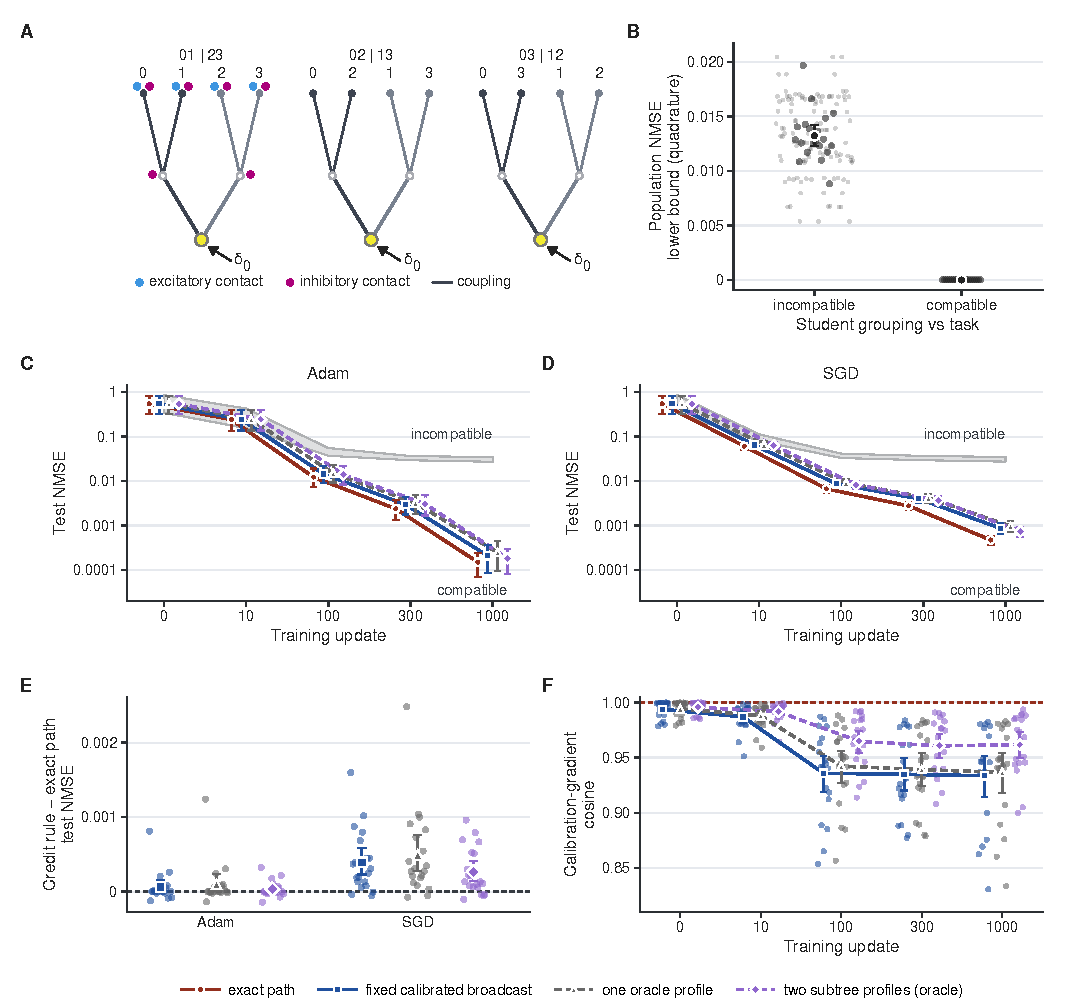
\includegraphics[width=\textwidth]{supplementary/curated/conductance_grouping.pdf}
\caption{\textbf{Input grouping and restricted feedback in positive-conductance trees.} \textbf{A}, Seven-compartment directed shunting model with the same physical shape, sixteen positive conductances (four excitatory and six inhibitory contacts plus six couplings) and soma-only readout under all three input groupings, $01|23$ (drawn), $02|13$ and $03|12$. Teacher-task permutations preserve the input-gradient spectrum. \textbf{B}, Analytic population lower bound from interactions crossing the student's two proximal input blocks, evaluated by converged quadrature. Dots average the six incompatible task/grouping pairs within each of twenty seeds; the mean bound is 0.013222 population normalized mean squared error (NMSE). Compatible groupings give exactly zero in all twenty seeds (one mark). This is neither an observed loss nor a certified numerical integration bound. \textbf{C,D}, Final held-out sample NMSE for exact path, fixed calibrated broadcast, one oracle profile and two subtree-profile credit rules under Adam and stochastic gradient descent (SGD), respectively. Filled circles average three compatible task permutations within seed; open squares also average the two incompatible groupings per task. Incompatible means are 0.029--0.032 NMSE, intervals narrower than the symbol. Rates were selected on development seeds and frozen before fresh outcomes. The fixed broadcast profile is calibrated from initial student path sensitivities, like the calibrated broadcast of main Fig.~4; projection coefficients access the current exact field and are oracle controls. \textbf{E}, Paired compatible-tree fixed-broadcast-minus-exact NMSE differences. The Adam interval includes zero; the small SGD effect does not establish a universal need for precise credit. Dots are the twenty independent seed means. Means and whiskers in \textbf{B--E} use 10,000 whole-seed bootstrap draws and pointwise 95\% intervals. Population-normalized bounds in \textbf{B} and split-variance-normalized test errors in \textbf{C--E} have distinct denominators. \textbf{F}, Mean aggregate gradient cosine on 256 calibration examples for compatible Adam models at the common exact-learning checkpoints 0, 10, 100, 300 and 1,000; no uncertainty band is shown, and means hide a 0.79--1.00 per-record range. Exact path is 1 by construction; fixed broadcast and one oracle profile coincide within 0.006. The interaction bound relies on independent input blocks, identity somatic activation and no direct somatic synapses; it is separate from the multi-affine cut-rank theorem. The rule colours of \textbf{C,D,F} and the key also mark subtrees and soma in \textbf{A}, incompatible (amber) and compatible (green) in \textbf{B}, and Adam (green) and SGD (amber) in \textbf{E}; main-text exact-path dark red is unused.}
\label{fig:si_conductance_grouping}
\label{fig:supp_morphology_conductance}
\end{figure}

\begin{figure}[p]
\centering
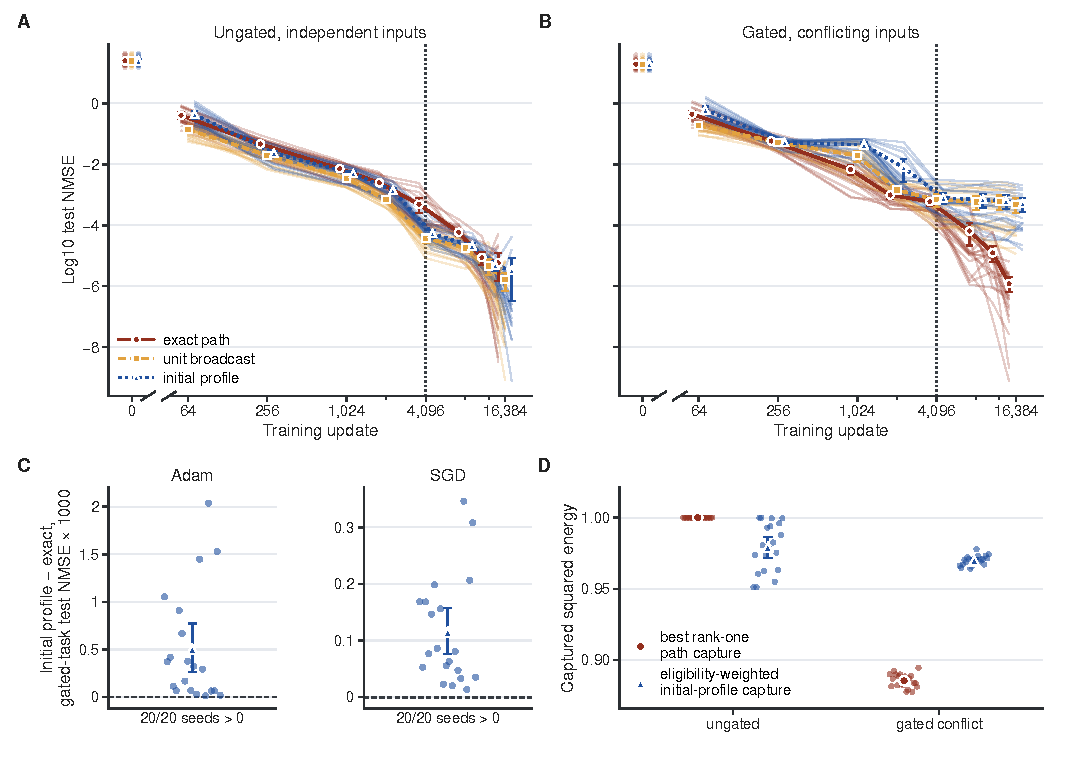
\includegraphics[width=\textwidth]{supplementary/curated/conductance_precision.pdf}
\caption{\textbf{A first conductance task produces a small precision benefit from exact credit.} \textbf{A,B}, Test normalized mean squared error (NMSE) under Adam at the nine saved checkpoints (0, 64, 256, 1,024, 2,048, 4,096, 8,192, 12,288 and 16,384 updates, joined by straight segments) for ungated independent inputs and gated conflicting inputs in the 16-conductance model, with exact-path credit, unit broadcast and the initial profile (the fixed calibrated broadcast). Curves show means and 95\% paired-seed bootstrap intervals across 20 fresh seeds; the vertical dotted line marks the original 4,096-update budget. All three rules share the initialization error (24.8 in \textbf{A}, 19.2 in \textbf{B}), above the drawn range; curves enter the frame before 64 updates. All fits continue to 16,384 updates with unchanged optimizer and minibatch state. On the ungated task the three rules are indistinguishable at 16,384 updates (exact $5.9\times10^{-6}$ [$1.5\times10^{-6}$, $1.2\times10^{-5}$], unit broadcast $1.6\times10^{-6}$ [$7.0\times10^{-7}$, $2.7\times10^{-6}$]); the precision benefit of exact credit is a gated-task effect. Unit-broadcast and initial-profile curves differ here because global gradient clipping can break Adam's invariance to fixed positive coordinate scaling. \textbf{C}, Gated-task NMSE differences, initial profile minus exact credit, at each fit's best validation checkpoint in the extended 16,384-update window, under Adam and under SGD, the latter at its separately selected rate with the same seeds and window. Points are the 20 paired seed differences; symbols and bars show their means and 95\% bootstrap intervals. The Adam gap is $0.000502$ [$0.000267$, $0.000772$] and the SGD gap is $0.000114$ [$0.000076$, $0.000157$], each positive in all 20 seeds; under Adam the mean gap thus stays below $6\times10^{-4}$ NMSE. \textbf{D}, Diagnostics at the exact-rule best-validation states distinguish the best rank-one capture of the six-compartment path field from capture by each student's fixed initial profile after weighting by local parameter eligibility. Both are squared-energy projection ratios with one freely fitted amplitude per example. Marks are means over 20 seeds with 95\% bootstrap intervals of the mean, narrower than the marker for three of the four points; ungated path capture is 1 by construction (effective rank 1.000 in every seed). High eligibility-weighted capture helps explain the small learning difference. Colours on this sheet: dark red is exact-path credit (\textbf{A,B}), the initial-profile-minus-exact gap (\textbf{C}) and rank-one path capture (\textbf{D}); orange is unit broadcast; blue is the initial profile (\textbf{A,B}) and eligibility-weighted profile capture (\textbf{D}); line style also separates the three rules in \textbf{A,B} (solid, dashed and dotted, in that order). Supplementary Fig.~\ref{fig:si_conductance_grouping} draws exact path green and fixed calibrated broadcast orange. The gated and ungated tasks change both inhibition and distractor dependence, so this first study is a task-family comparison. All 216 development fits, 240 fresh fits and their continuations are retained in Source Data.}
\label{fig:si_conductance_precision}
\label{fig:supp-conductance-small-effect}
\end{figure}

\begin{figure}[p]
\centering
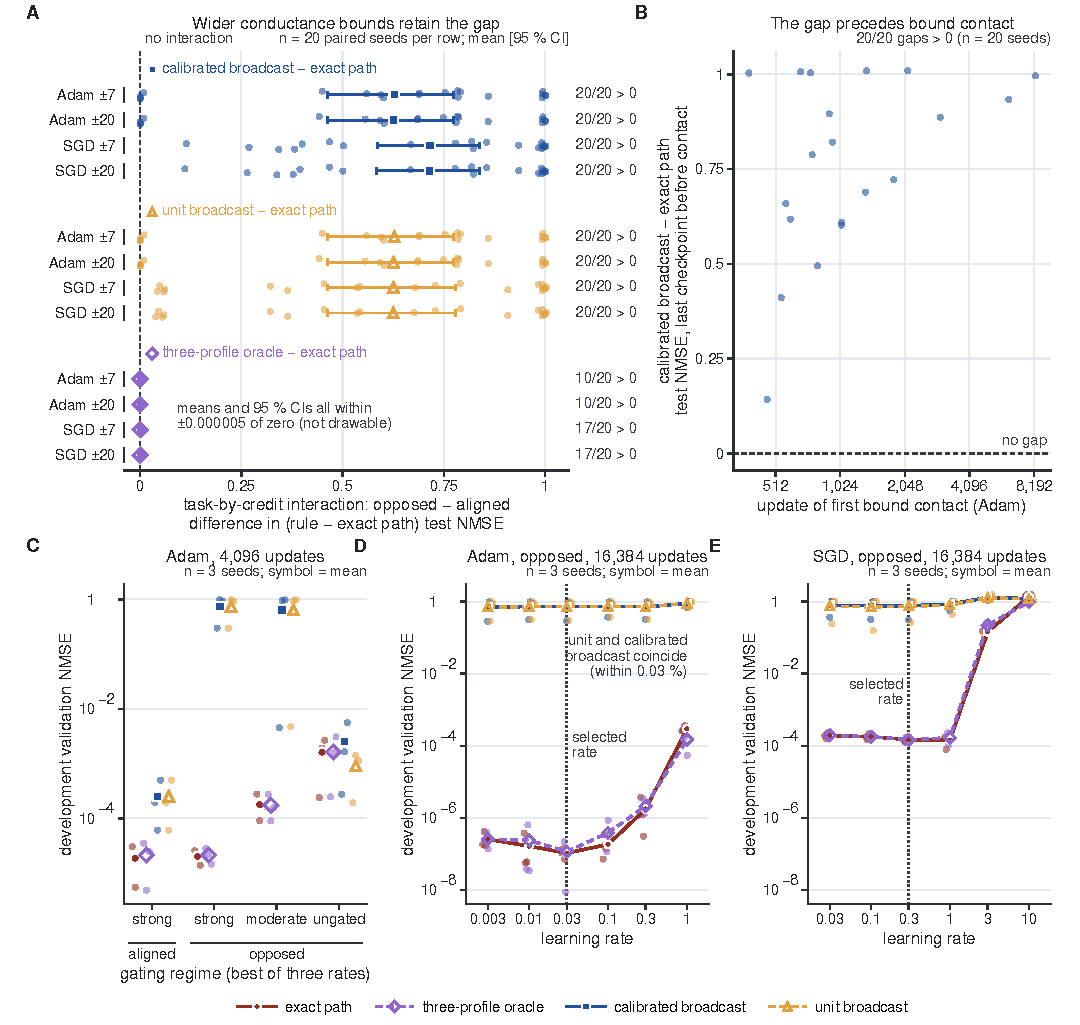
\includegraphics[width=\textwidth]{supplementary/curated/conductance_optimization.pdf}
\caption{\textbf{Parameter-range, development and rate controls retain the opposed-task broadcast deficit.} \textbf{A}, Task-by-credit interaction (opposed minus aligned calibrated-broadcast-minus-exact NMSE) under original $[-7,7]$ (open circles) and wider $[-20,20]$ (filled squares) log-conductance bounds with Adam and SGD; fits run to 16,384 updates. Symbols are twenty-seed means, bars 95\% paired bootstrap intervals; every seed is positive. Unit-broadcast rows are within 13\% and oracle rows below $4\times10^{-6}$. \textbf{B}, Initial-profile-minus-exact NMSE at each seed's last saved checkpoint before its fit first reaches an original bound: one dot per seed, no interval; all twenty are positive, and eleven share the 256 column, leaving seventeen visible marks. \textbf{C}, Four development regimes under Adam at the original 4,096-update budget (each rule's best of three rates; three development seeds): aligned strong, opposed strong, opposed moderate (parent inhibition one) and opposed ungated (zero); exact and oracle marks agree within 13\%, and the broadcast pair coincides except when ungated. \textbf{D,E}, Six-rate opposed-tuning sweeps under Adam and SGD at a 16,384-update budget, so exact-path values are lower than in \textbf{C} ($1.0\times10^{-7}$ against $2.0\times10^{-5}$ at Adam rate 0.03); dotted lines mark the originally selected rates. Points are three-seed means without error bars; seed ranges span up to a factor of 25, far below the three-decade rule separation at rates up to 1, and unit broadcast and initial profile coincide within 7.4\%. The improvement trigger was not reached; aligned sweeps and all 288 outcomes are in Source Data. Colours: dark red exact path (as in main Fig.~4), purple three-profile oracle, orange unit broadcast, blue open squares initial profile (main Fig.~4's calibrated broadcast); the dark red of \textbf{A} and lighter blue of \textbf{B} are not rule colours. Some broadcast fits reach the wider bounds; these are finite-budget controls, not a convergence proof.}
\label{fig:si_conductance_optimization}
\label{fig:supp-conductance-robustness}
\label{fig:supp-conductance-expanded-rates}
\end{figure}

\begin{figure}[p]
\centering
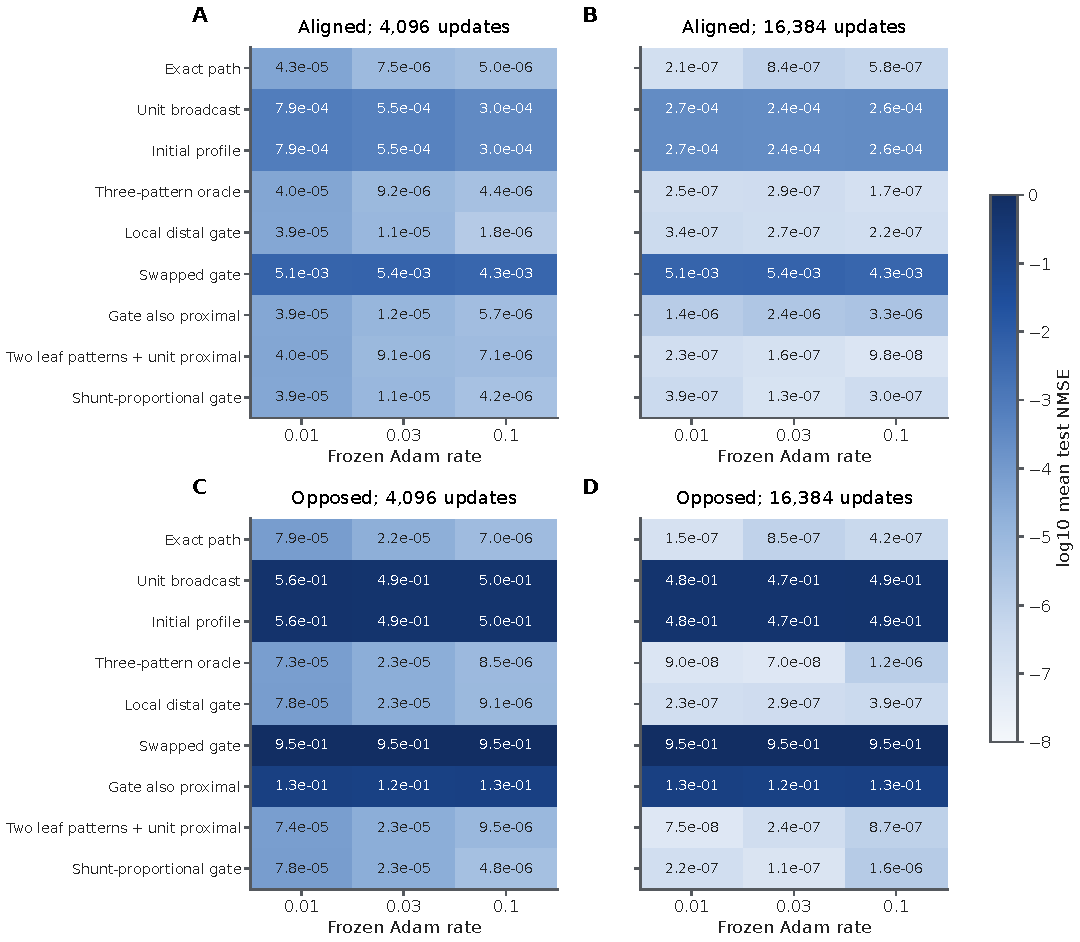
\includegraphics[width=\textwidth]{supplementary/curated/local_gate_controls.pdf}
\caption{\textbf{Local conductance gating is robust to rate choice but depends on where it is applied.} \textbf{A,B}, Aligned tuning at 4,096 and 16,384 updates. \textbf{C,D}, Opposed tuning at the same budgets. Every rule receives each of the three Adam rates on the x axis, fixed (`frozen') before the confirmatory seeds were run; the middle column, 0.03, is the primary rate and the outer columns are robustness conditions. Each cell prints the arithmetic mean test NMSE at validation-selected checkpoints over $n=20$ new paired seeds and is filled by the base-ten logarithm of that same number on the bar at right (0 is NMSE 1; $-8$ is $10^{-8}$). No interval is drawn: per-cell medians and 95\% whole-seed bootstrap intervals are tabulated in Source Data (\texttt{condition\_means.csv}), and the within-cell seed spread of $\log_{10}$ NMSE (median s.d. 0.54 decades) means that differences of less than about a decade between rows are not resolved by this table; the fill resolves only the failed-versus-accurate split, so finer comparisons are read from the printed digits. Row labels are those of the frozen render; in the vocabulary of main Fig.~5, `Initial profile' is the calibrated broadcast (profile fixed from the initial exact path factors), `Local distal gate' is the distal gate, `Gate also proximal' is the also-proximal placement and `Two leaf patterns + unit proximal' is the two-profile oracle. Unit broadcast and calibrated broadcast (`Initial profile') are two rules whose means agree to two significant figures in every cell, so the two rows are drawn identically and are read as one broadcast row; individual seeds differ by up to 3.1-fold between them. Exact path, the three-pattern oracle, the local distal gate and the shunt-proportional gate learn accurately. Swapping the gate fails; extending the gate to proximal compartments leaves a substantial opposed-task deficit. The two leaf patterns with unit proximal feedback isolate this placement effect. On the aligned task at 16,384 updates the gate-also-proximal means ($1.4$--$3.3\times10^{-6}$) are raised 17--25-fold above their medians ($0.8$--$2.0\times10^{-7}$) by one or two outlier seeds, and those medians match the accurate rules' ($0.5$--$1.9\times10^{-7}$), so the darker fill of that row in \textbf{B} is an outlier effect, not an aligned-task deficit; smaller outlier inflation (about tenfold) affects the two-leaf oracle at 0.03 and the shunt-proportional gate at 0.1 in \textbf{D}. These are supplied-context, bounded-conductance experiments; the local gate does not estimate arbitrary route coefficients. Both budgets and all rates and seeds remain included; the historical cancellation cohort of the same study is drawn at the main-text type scale in main Fig.~5G.}
\label{fig:si_local_gate_controls}
\label{fig:supp_local_gate_controls}
\end{figure}

\clearpage

% Curated from paper commit 7ee9157; scientific protocols are unchanged.
\section{Serial physical computation and training budgets}
\label{note:depth}

\subsection{Generator, architecture and primary comparison}
The \texttt{hierarchical\_gain\_load} task supplies 64 positive excitatory and 64 positive inhibitory rates. Fine, coarse and global Gaussian node fields generate three mean-corrected lognormal gain factors (hierarchy H3). The product of these factors modulates distal class-bearing excitation; separate inhibitory sensor blocks report each factor. For a signal-bearing coordinate,
\begin{equation}
 x_E=\max\{b_E+y\Delta+\epsilon_E,10^{-4}\}
 \exp\!\left(\sum_{\ell=1}^{3}\sigma_\ell z_\ell-
                 \tfrac12\sum_{\ell=1}^{3}\sigma_\ell^2\right),
 \label{eq:s_task_family_nested}
\end{equation}
where $y\in\{0,1\}$ is balanced class, $\Delta=0.80$, $\sigma_\ell=0.25$, $z_\ell$ are independent standard Gaussians and $\epsilon_E$ is independent Gaussian noise of SD 0.08. The same noise--floor--gain order applies to inhibitory rates. Class-independent middle/proximal excitation has baseline 0.02, so flooring makes its effective rate noise nonzero-mean. Each dataset contains 10,000 balanced examples.

Sensor alignment $\alpha$ changes correspondence without changing marginal Gaussian variance:
\begin{equation}
 s_\ell(\alpha)=\alpha z_\ell+\sqrt{1-\alpha^2}\,\xi_\ell,
 \qquad \xi_\ell\overset{\rm iid}{\sim}\mathcal N(0,1),
 \label{eq:s_task_family_alignment}
\end{equation}
with sensor noise independent of latent gains. Alignment uses $\alpha=1$; independent sensors use zero. A nonzero cyclic trial shift instead removes trial-specific access while preserving the entire inhibitory field. Reversed placement exchanges fine/global feature ranges across inventory tiers, preserving their 21/22/21 widths. An earlier three-cycle assignment changed candidate slots and was excluded before inference.

Branch factors run soma to distal. For factors $[b_1,\ldots,b_D]$, the nonsomatic count is $\sum_{j=1}^D\prod_{r=1}^jb_r$. D1 $[8]$, D2 $[2,3]$ and D3 $[2,1,2]$ each contain eight units per soma; D3's unary middle stage preserves that inventory. Structured masks place all tiers in D1, fine/coarse distally and global proximally in D2, and one tier per stage in D3. Every architecture has 66,178 trainable parameters, 14,336 active synapses, 21,760 candidate slots and 2,944 persistent state scalars per sample. Compartments use the directed positive-conductance division, identity reactivation and softplus-positive synapses.

Excluded calibration seeds 10100--10141 tested signal contrast, gain shift and child conductance. Contrast 0.24 with train/test gain SD 0.25/1.2 remained at chance despite improved training fits at depth. Coupling and contrast sweeps selected child conductance 16, contrast 0.80 and matched SD 0.25; contrast 0.72 missed the predefined D1 accessibility threshold (two-seed mean test accuracy at least 0.60 at every depth; D1 reached 0.597 at contrast 0.72 versus 0.609 at contrast 0.80). All failed calibration settings remain in Source Data.

The primary 270 fits crossed D1--D3, ten paired seeds 10200--10209 and nine conditions: aligned shunting BP; independent-sensor, shuffled-sensor or reversed-placement BP; aligned raw-additive BP; and aligned/reversed LocalCA with shared-soma or exact-path credit. The protocol required at least 9/10 aligned-BP seeds above 0.55 at every depth and every mean below 0.98. All conditions passed completeness, finite-metric, resource and no-fallback checks. Training used a 180-epoch cap and validation-loss early stopping with patience thirty. The BP recipe used Adam at 0.003; LocalCA retained split parameter groups with nominal rate 0.0008. Group rates, boosting, decay and update options are retained in the resolved configurations.

At that budget, aligned-BP D3 minus D1 was 30.86 percentage points; alignment-minus-control depth interactions exceeded 30 points. Aligned additive BP declined with depth. These contrasts separate forward composition from a credit-rule effect, whose budget dependence is evaluated below. A post hoc common-checkpoint audit found exact-path LocalCA gradients collinear with autograd (minimum cosine $0.9999999999994$), while shared-soma cosine declined from 0.946 at D1 to 0.767 at D3. This gradient diagnostic does not establish a converged learning requirement.

\subsection{Nonserial and point-model controls}
An all-active grouped star retains branch layers, masks and parameters but lets each nonsomatic layer read external inputs independently; child-aggregation parameters contribute only once at the soma. D1 logits match exactly. A literal grouped-point control additionally replaces child aggregation by direct projections to the soma, copying the corresponding initial scalar conductances. These controls retain resource counts while removing serial inheritance of branch states.

The star/point/credit-coordinate study comprised 200 fits on the same ten H3 seeds: 140 initial controls and sixty optimizer-matched soma-broadcast fits. Serial exceeded star by 30.81 percentage points at aligned D3 (95\% paired interval, 30.41--31.26), but fell below it by 0.43 points after reversal. Two unconstrained point MLPs matched active parameters (15,055) or nearest realizable total parameters (66,200 versus 66,178). At the 180-epoch budget, their mean accuracies, 0.9861 and 0.9902, exceeded the tree. This finite-budget comparison does not establish a final performance ceiling for the tree; its D3 exact-BP mean reached 0.99998 at ordinary stopping.

Soma-broadcast autograd preserves local synaptic derivatives but replaces nonsomatic loss derivatives by each unit's somatic derivative. Full BP exceeded it by 0.64 percentage points under the BP optimizer. Under the LocalCA optimizer, broadcast autograd and shared-soma LocalCA differed by only $-0.06$ points ($-0.23$ to 0.09), whereas changing the broadcast optimizer cost 13.47 points at 180 epochs. The optimizer-matched comparison was specified after discovering the recipe difference. It isolates that implementation contrast; autograd is not a biological mechanism. Full configurations and outcomes are in \texttt{source\_data/point\_dendrite\_credit\_controls/}.

Sixty additional literal grouped-point H3 fits used aligned/reversed placement and D1--D3 on the same seeds. Grouped-point means remained near 0.61 across depth. Serial-minus-grouped at aligned D3 was 30.87 points, reversing to $-0.44$ under placement reversal. These observations agree with the star control without retaining its child-aggregation modules.

\subsection{Alignment, hierarchy and task-family sensitivities}
The alignment interpolation was specified after endpoint outcomes but before intermediate fits. Ninety runs crossed $\alpha=0.25,0.50,0.75$, three depths and the original ten seeds. D3-minus-D1 effects at $\alpha=0,0.25,0.50,0.75,1$ were 0.019, 0.207, 0.820, 3.126 and 30.855 percentage points. The prespecified within-seed linear summary had mean slope 25.84 points per unit alignment, but the final interval contributed 27.73 points: the response is strongly nonlinear. Software records identify an unused optional-rule edit; all unique conditions passed resource checks (\texttt{source\_data/\allowbreak physical\_\allowbreak alignment\_\allowbreak dose/}).

The H2 follow-up fixed two 32-feature tiers, inventory 4/4 and D1 $[8]$/D2 $[4,1]$ before outcomes. Ten new seeds 10300--10309 crossed aligned/reversed placement, serial or literal grouped-point BP, and shared-soma or exact-path LocalCA (160 fits). No inherited signal, conductance or optimization setting was retuned. Aligned serial BP gained 30.84 points from D1 to D2; the placement interaction was 32.40 points. Grouped-point depth effects remained near zero. This is replication within the same synthetic mechanism family. Together with the sixty H3 grouped-point fits, all 220 outcomes are in \texttt{source\_data/\allowbreak remaining\_\allowbreak physical\_\allowbreak experiments/}.

H4 used four 16-feature tiers, inventory $[4,2,1,1]$ and D1--D4, adding D4 $[1,1,2,2]$. All depths retain the same eight-unit resources. The 360 fits crossed aligned/reversed placement, serial/grouped-point BP, both LocalCA rules and aligned raw-additive BP over seeds 10400--10409. An automatic D3 partition error stopped ninety configurations before outcomes; explicit grouping $[4],[2],[1+1]$ restored the intended counts, and only failed configurations were repeated. The main contrasts, 50,000-draw intervals, exact sign-flip tests and BH family were specified before analysis, with positive claims additionally requiring 8/10 concordant signs. Aligned BP accuracy peaked at D3: D4 minus D3 was $-1.46$ points ($-1.74$ to $-1.16$), although D4 minus D1 remained 25.63 points. This falsified the predefined simple depth-equals-hierarchy crossover. Exact-path LocalCA's 0.60-point D4--D3 gain failed the direction criterion (7/10); the shunting-minus-additive increment was also inconclusive. All reversed and null endpoints remain in \texttt{source\_data/physical\_depth\_h4\_factorial/}.

A paired additive-placement follow-up completed both placements at all three H3 and four H4 depths (140 fits, the original seeds and 180-epoch recipe). Neither placement reproduced the strong shunting depth benefit. Placement nevertheless mattered at H4: the depth-by-placement interaction was positive because reversed-placement accuracy declined with depth while aligned accuracy remained near chance (9.00 percentage points, 95\% paired interval 5.66--12.58; Holm-adjusted $P=0.0039$). The H3 interaction was inconclusive ($-2.65$ points, $-7.63$ to 3.18). Thus sensor placement can affect additive models too; the distinctive shunting result is successful serial computation under the matched placement. These same-seed sensitivity analyses, their frozen protocol and all 140 outcomes are retained in \texttt{source\_data/additional\_figure\_controls/}.

A same-seed computational repeat under source commit \texttt{a99c3a7} covered all 220 H2/grouped-point fits and 210 principal H3 fits. Median absolute accuracy drift was 0.030 percentage points, mean drift 0.154 and maximum drift 15.01 in a raw-additive control; 357/430 pairs were within 0.1 points. Principal shunting and local-credit directions persisted. Supplementary Table~\ref{tab:physical_reproducibility} retains this unfavorable reproducibility range; these reused seeds are not fresh replication.

The fixed-D3 task-family study used seeds 10500--10509 and crossed three generators, $\alpha=0,0.5,1$, serial and grouped-point composition and BP or exact-path LocalCA (360 fits). Nested factors use Eq.~\ref{eq:s_task_family_nested}. Flat factors retain the same product and marginal variances but assign each independent factor to the same deterministic eight-bin spatial partition. Local-ratio inputs give excitation and inhibition at each level correlated cumulative hierarchical fields, making divisive information locally available. All families retain 10,000 balanced examples, distal-only class signal and identical model resources. Primary architecture-by-alignment and between-family contrasts used 50,000 paired bootstrap draws and an 8/10 sign criterion. BP alignment interactions were 30.41, 22.26 and 1.30 percentage points for nested, flat and local-ratio tasks; LocalCA effects were 27.70, 12.37 and $-11.68$. The local-ratio reversal is retained in \texttt{source\_data/task\_family\_alignment/}.

\subsection{Longer training and metric dependence}
The original 180-epoch cohort and a subsequent 600-epoch restart study left all fifty D3 fits at their caps with decreasing validation loss. The latter used four GPU and six CPU seed blocks, matched across conditions within each seed. Its complete outcomes remain in \path{source_data/physical_depth_budget/} and \path{source_data/physical_depth_followup/}; these finite-budget results are superseded for the stopping comparison in main Fig.~7E--H.

The completed extension retained all six configurations and ten original seeds (10200--10209), frozen implementation \texttt{a99c3a7}, optimizer settings and thirty-epoch validation-loss patience, now using H200 GPUs throughout. Ten already stopped fits were retained. Seven runs resumed verified weights, optimizer, global random states and private data-loader generators; forty-three restarted the original seeds after launch or storage failures. Within each configuration, only output locations and the safety cap changed. The execution protocol records these differences. All sixty runs reached ordinary early stopping before their safety caps: 6,000 epochs for the ten retained runs and 24,000 for the fifty resumed or restarted runs.

D1 stopping epochs ranged from 110 to 746; D3 epochs ranged from 3,082 to 9,674. Every final model matched its validation-selected checkpoint exactly. Test metrics never selected settings or states. Curves carry stopped validation-best states forward, retaining ten seeds in each mean. The analysis retains every observed epoch and displays every epoch through 600, then a fixed logarithmic grid plus budget and stopping epochs. Intervals use 10,000 whole-seed bootstrap draws and are descriptive and pointwise.

Exact-BP D3 minus D1 accuracy at stopping was 38.869 (38.640 to 39.115) percentage points. The LocalCA exact-minus-shared accuracy difference changed from 10.96 points at epoch 180 to $-1.534$ ($-1.826$ to $-1.244$) at epoch 600, then returned to 0.150 (0.122 to 0.179) at stopping (10/10 positive seed differences). Exact-path LocalCA also retained lower final test cross-entropy: 0.0010 versus 0.0112 nats for shared-soma LocalCA, a paired difference of $-0.010$ ($-0.012$ to $-0.008$) nats. Thus the intermediate accuracy reversal was transient; the final difference was small in accuracy but clearer in loss.

The broadcast BP-minus-LocalCA recipe effect on accuracy shrank from 13.45 percentage points at epoch 180 to 0.02 ($-0.02$ to 0.06; 7/10 positive seeds) at ordinary stopping. Under the BP recipe, exact BP retained a small advantage over soma-broadcast autograd: 0.14 points (0.10 to 0.17; 10/10 positive seeds) and a test cross-entropy difference of $-0.013$ ($-0.017$ to $-0.009$) nats. These are paired means with descriptive 95\% bootstrap intervals.

\path{source_data/physical_depth_stopping_extension/} contains the frozen extension protocol, complete training histories, validation-selected seed trajectories, checkpoint and metric-file audits, paired contrasts and historical restart comparisons. The GPU restarts need not exactly reproduce the earlier mixed-device trajectories; budget comparisons use windows of the same new run. Reusing the original seeds makes this a stopping sensitivity analysis, not fresh independent confirmation. Ordinary early stopping does not prove global optimization convergence.

\begin{figure}[p]
\centering
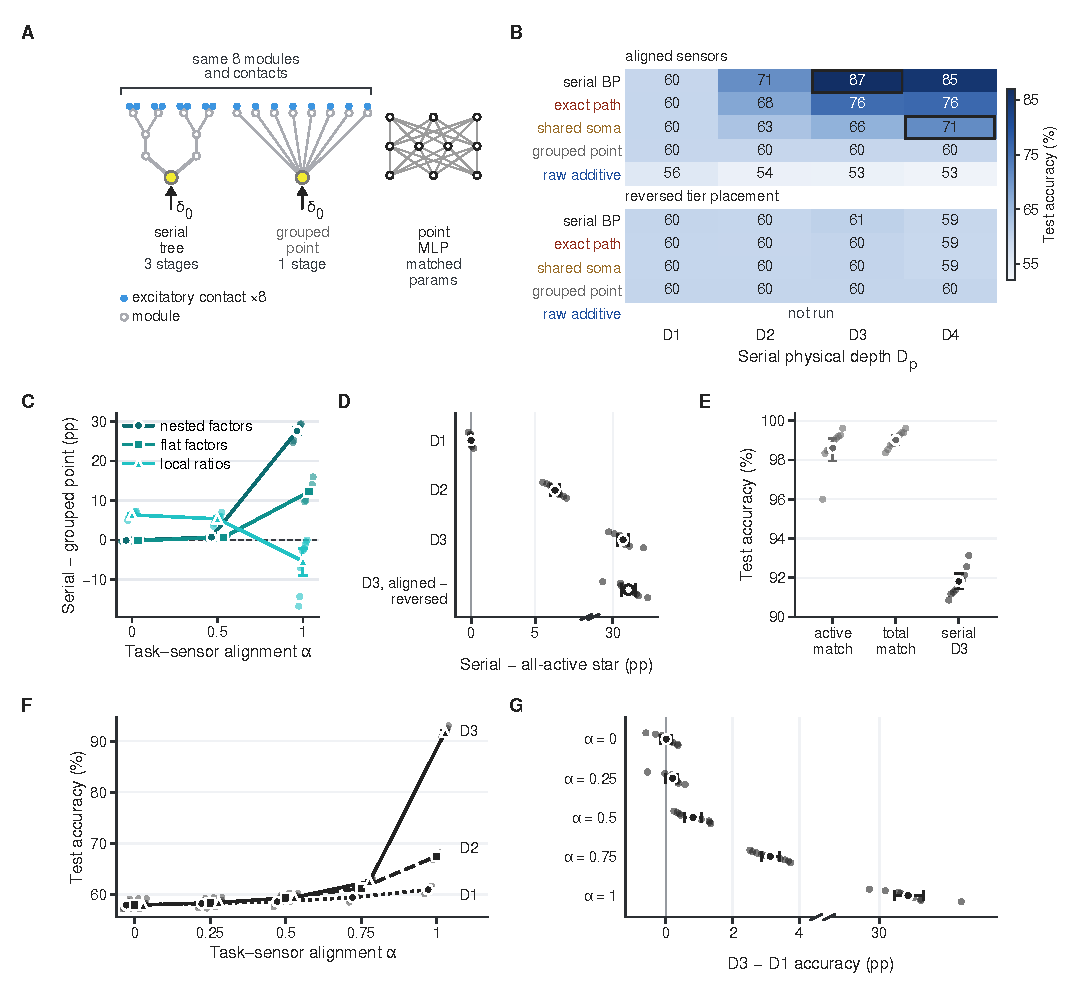
\includegraphics[width=\textwidth]{supplementary/curated/physical_architecture.pdf}
\caption{\textbf{Task-matched serial computation differs from grouped and flexible point controls.} \textbf{A}, Serial D3, resource-identical grouped-point and approximately parameter-matched flexible point networks. Only serial/grouped models share modules and contacts. \textbf{B}, Original-budget three-level aligned task across D1--D3 and feedback rules. \textbf{C}, Four-level task across D1--D4 under aligned/reversed sensor placement. \textbf{D}, Serial-minus-grouped accuracy at fixed D3 across nested, flat and local-ratio task families, under exact-path LocalCA. \textbf{E}, Serial-minus-grouped-star effects and their alignment interaction. \textbf{F}, Flexible point controls matched to active or total parameter count. Curves and differences use ten paired seeds per cohort and 95\% paired-seed bootstrap intervals. These task-calibrated, original-budget comparisons establish forward-computation dependence on task/placement, not an optimizer-independent requirement for resolved credit. Main Fig.~6 shows the longer-budget accuracy reversal and cross-entropy trajectory.}
\label{fig:si_physical_architecture}
\label{fig:supp_physical_depth_controls}
\label{fig:physicaldepth}
\end{figure}

\begin{figure}[p]
\centering
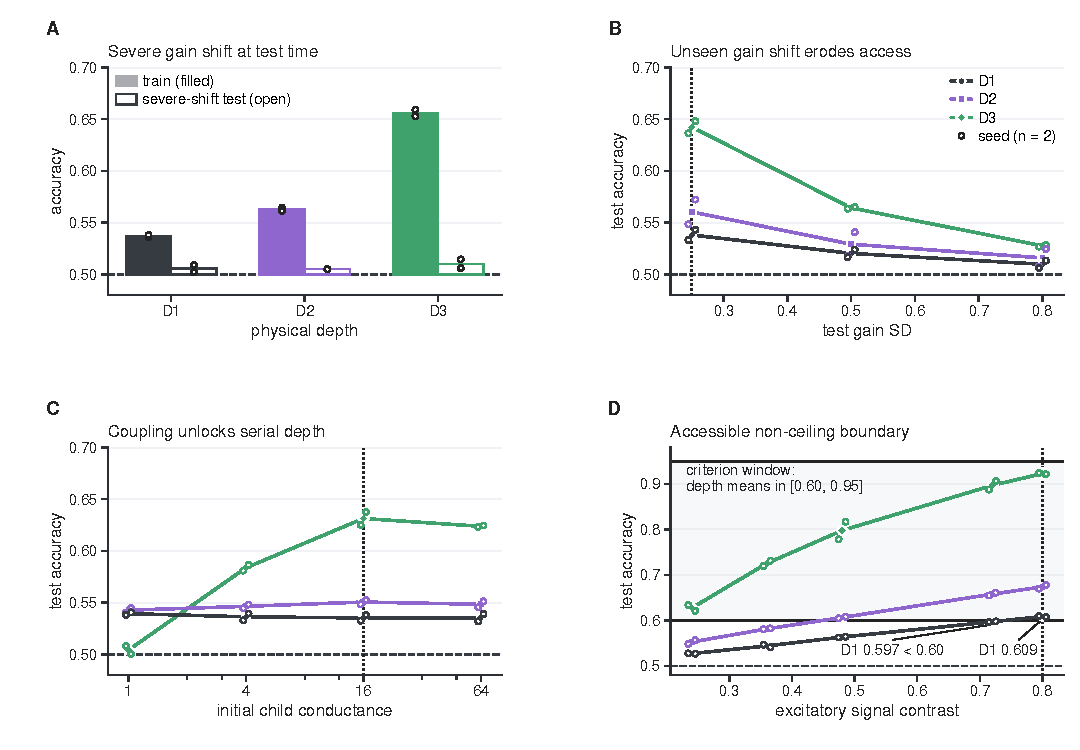
\includegraphics[width=\textwidth]{supplementary/curated/physical_calibration.pdf}
\caption{\textbf{Transparent calibration of the nonlinear physical-depth operating point.} All panels use the three-level hierarchical gain-load task and serial shunting morphologies D1 \([8]\), D2 \([2,3]\) and D3 \([2,1,2]\), each with eight nonsomatic compartments per soma. They test the prerequisite for the main hypothesis: whether the mechanism-matched divisive task is accessible at every depth before comparing depth benefits. \textbf{A}, The original aligned shunting-backpropagation (BP) pilot at signal contrast 0.24 fit the training distribution increasingly with depth but remained at chance under the prespecified severe gain shift (test gain standard deviation (SD) 1.2). Bars are two-seed means and dots are the individual exploratory seeds. \textbf{B}, With training gain SD fixed at 0.25, increasing unseen test gain variation eroded accessibility at every depth. The dotted line marks the matched train/test condition. \textbf{C}, At matched gain and signal contrast 0.24, stronger child coupling selectively made serial D3 computation accessible; the dotted line marks child conductance 16 used subsequently. \textbf{D}, At matched gain and child conductance 16, increasing excitatory signal contrast moved D1--D3 away from chance without saturating D1 or D2. The separately run 0.80 boundary (dotted line) met the predefined accessibility criterion and selected the operating point used for the analysis seeds. Lines show two-seed means; shading spans the two exploratory values and is not a confidence interval. All pilot, ladder and boundary seeds were excluded from the confirmatory contrasts.}
\label{fig:si_physical_calibration}
\label{fig:supp_nonlinear_depth_calibration}
\end{figure}

\begin{figure}[p]
\centering
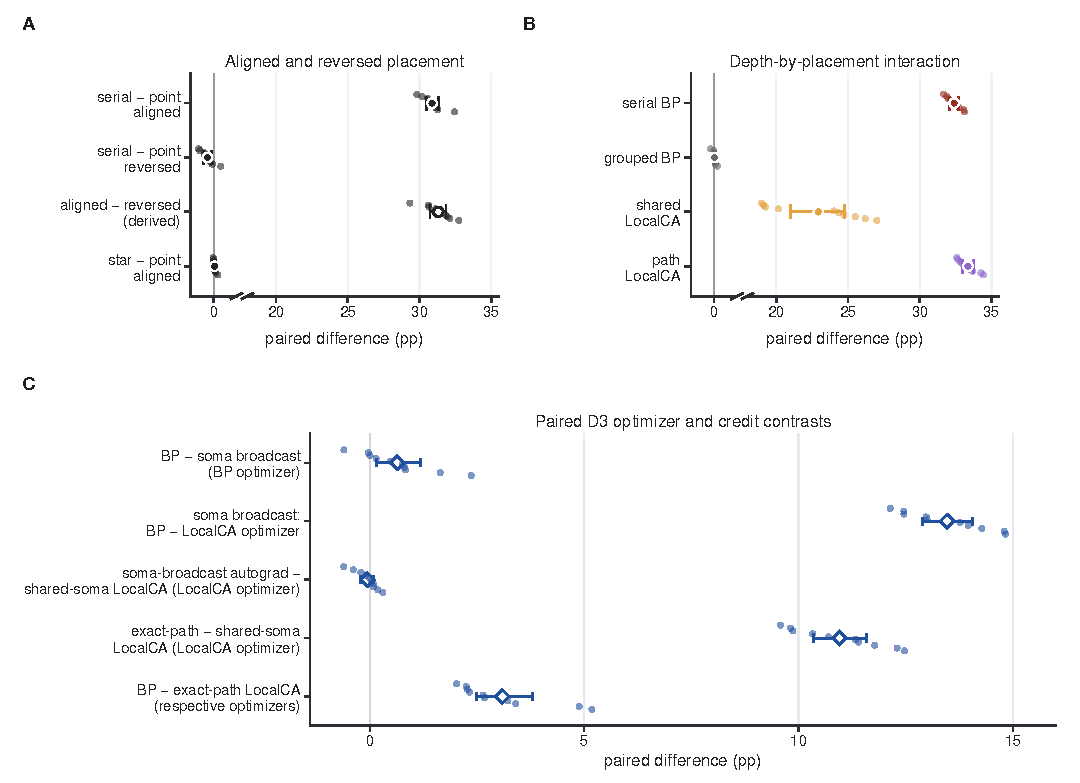
\includegraphics[width=\textwidth]{supplementary/curated/physical_optimizer.pdf}
\caption{\textbf{Physical-depth conclusions depend on alignment, task hierarchy and optimization.} \textbf{A}, Serial/point contrasts under aligned and reversed placement. \textbf{B}, Separate two-level task: depth-by-alignment interactions for serial/grouped-point backpropagation and shared/exact LocalCA. \textbf{C}, Original-budget D3 optimizer/credit-coordinate contrasts. Under the BP optimizer, full versus soma-broadcast differentiation differs by 0.64 points; under the split LocalCA optimizer, exact versus shared differs by 10.96 points; changing the broadcast optimizer costs 13.47 points. Means and intervals use ten paired seeds and 95\% bootstrap intervals. These earlier recipe-specific effects do not imply a converged credit advantage: at 600 epochs the LocalCA accuracy difference reverses, while exact credit retains lower cross-entropy (main Fig.~6). All D3 continuations hit the cap; D1 usually stops early.}
\label{fig:si_physical_optimizer}
\label{fig:supp_physical_depth_diagnostics}
\end{figure}

\clearpage

% Curated from paper commit 7ee9157; scientific protocols are unchanged.
\section{Anatomical dictionaries and controlled field alignment}
\label{note:anatomical_dictionaries}

\subsection{Reconstruction, cohorts and electrical normalization}
\label{note:microns}
The initial cohort comprises eight layer 2--5 intratelencephalic cells from MICrONS \citep{microns2025}. Stable nuclei were resolved in \texttt{minnie65\_public} materialization 1822; skeletons came from the MICrONS skeleton service and incoming contacts from \texttt{synapses\_pni\_2}. Degree-two chains were collapsed to branch-to-branch cables. Contacts were assigned to the nearest dendritic node and retained within $5\,\mu$m. Across cells, 28,669 E/I-classified contacts passed, with mean mapping fraction 0.980. Root traversal checked acyclicity and a unique path to the soma. Cell identifiers, contact counts and source assets are indexed in Supplementary Table~\ref{tab:source_index}.

Presynaptic coarse type supplied E/I identity where available. Otherwise the in-development \path{synapse_target_predictions_ssa_v2} table classified high-confidence spine targets as excitatory and shaft/soma targets as inhibitory. This proxy table lacks a stable public release identifier. Direct/proxy agreement was 73.01\% among 2,012 jointly labeled contacts (E/E 489, E/I 84, I/E 459, I/I 980). Principal comparisons were repeated on the 2,077 directly typed contacts. Coverage and error asymmetry are observed properties, not missing-at-random assumptions.

A non-overlapping robustness cohort was defined from a 55-cell convenience export before outcomes, resolved in public v661 and excluding the original eight by stable nucleus. Its 47 retained cells are from the same mouse and an earlier reconstruction release. Direct presynaptic labels were available for 11,024 incoming contacts (4.71\%) before mapping; 10,516 mapped contacts entered analysis. This layer-imbalanced cohort is not a population or independent-animal replication.

The second-animal cohort used published Pinky v185 mesh, soma-valence and dense-synapse data \citep{turner2022neocortex,microns_pinky_v185}. Before mesh or selected-cell contact counts were inspected, 362 excitatory soma rows were ordered along the second volume coordinate and split into twelve equal-count strata. Each stratum contributed the root nearest the global first/third-coordinate medians, with root-ID tie-breaking. This deterministic rule spans the volume while reducing boundary truncation; it is not random sampling. Mesh processing retained the largest face-plus-link-edge component and used meshparty TEASAR with $7.5\,\mu$m soma collapse and $12\,\mu$m invalidation. Radius was half the opposite-surface ray distance at mesh anchors (\texttt{embreex} 2.17.7.post7). Only presynaptic roots labeled in the published soma-valence table supplied E/I identities.

Pinky inherited v661 compression, mapping, normalization, dictionary ranking and 500-shuffle settings. Inclusion required at least twenty mapped typed inputs and three inhibitory inputs. All twelve cells processed; ten qualified, with excluded cells having nineteen and thirteen inputs. Their route-generated $K=4$ ancestry advantages over random routes, depth bins and shuffling agreed in direction with the other mouse. Cell-bootstrap intervals describe stability within each volume; two mice do not support a population-level animal test. In the equal-broadcast analysis below, only eight Pinky cells qualify at $K=8$ and none at $K=16$; lower-budget results retain the other eligible cells.

Raw axial coupling scales as radius squared over length, divided by its within-cell positive median and clipped to 0.05--20. Leak scales as radius times the larger of length and radius, similarly normalized and clipped to 0.1--10. Synaptic areas are divided by the median nonzero total area. These are normalized passive sensitivity weights, not fitted membrane conductances. The reconstructed model uses reciprocal coupling and a symmetric conductance matrix; the directed path product of Eq.~\ref{eq:s_path_gain} applies only to the artificial network.

For excitatory-bearing segment $i$ and inhibitory-bearing route site $k$, define
\begin{equation}
 \Gamma_{ik}=A_{ik}\beta_k,
 \label{eq:s_kernel}
\end{equation}
where $A_{ik}$ indicates that $k$ lies on the path from $i$ to soma and $\beta_k$ is its normalized inhibitory fraction. This ancestry kernel approximates route weighting; it is not the reciprocal Green's-function derivative. Excitatory-area-weighted singular values $s_j$ give participation rank $(\sum_js_j^2)^2/\sum_js_j^4$.

\subsection{Mapping, labels and cable compression}
\label{note:morphology_uncertainty}
The eight-cell uncertainty analysis crosses mapping thresholds 2, 5 and $10\,\mu$m with direct-only or hybrid labels (proxy probability at least 0.8). Radius factors are $\exp(\sigma_r z-\sigma_r^2/2)$ for independent standard Gaussian $z$, with $\sigma_r=0,0.25,0.5$ and five paired draws at each nonzero dose. Every condition reselects up to four routes by the same leverage. Jaccard overlap measures route changes; capture uses the fixed nominal field, sites and weights, isolating dictionary sensitivity rather than changing both sides of the comparison.

Compression preserves total length and length--radius product to rounding error, but mean-radius resistance $\ell/\bar r^2$ differs from the series sum $\sum_e\ell_e/r_e^2$. Median relative error was $-0.00200$, with minimum $-0.99717$. A second normalization uses inverse series resistance, retaining leak, synapses and clipping; radius perturbations rescale resistance inversely with squared radius. All 1,056 conditions remain. Nominal mean capture was 0.3293 under mean-radius and 0.3375 under series normalization; small mean changes do not negate substantial local resistance errors. Draws were averaged within cell and intervals used 5,000 cell resamples. Audits and cache hashes are in \texttt{source\_data/review\_morphology\_uncertainty/}.

\subsection{Route-generated capacity and spatial scales}
\label{note:structural_capacity}
Route-generated fields multiply independent amplitudes by Eq.~\ref{eq:s_kernel}. Dictionaries comprise a dense PCA oracle, selected real ancestry routes, random nonempty routes, cable-depth bins and independently shuffled ancestry columns preserving values and sparsity. Real routes rank by inhibitory fraction times descendant excitatory-area fraction. Fields and dictionaries are both transformed by square-root excitatory area before least squares (Eq.~\ref{eq:s_capture}). Twenty Monte Carlo streams each contain 384 fields and 64 randomized dictionaries per cell and budget; streams are averaged within cell before inference.

At $K=8$, original ancestry capture was 0.487 with 6.92\% dense wiring. The same model-matched construction favored ancestry in the direct-label subset and all 47 non-overlapping cells. These positive controls measure internal compressibility of the route family. The older replication reports one minus residual norm, which differs from squared-energy capture; Source Data retain each endpoint's definition.

A deterministic unbalanced tree-Haar basis tests route scales on all 55 cells, with the 47-cell cohort primary. A region $R$ is split at the descendant subtree closest to half its excitatory weight, giving $A\dot\cup B=R$. For site weights $w_i$ and region sums $W_A,W_B,W_R$,
\begin{equation}
 h_{R,i}=\begin{cases}
 \sqrt{w_i}\sqrt{W_B/(W_AW_R)},&i\in A,\\
 -\sqrt{w_i}\sqrt{W_A/(W_BW_R)},&i\in B,\\
 0,&i\notin R.
 \end{cases}
 \label{eq:s_irregular_haar}
\end{equation}
With $h_{0,i}=\sqrt{w_i/\sum_jw_j}$ these contrasts form a complete orthonormal basis \citep{gavish2010wavelets}. All bases were full rank, with maximum orthonormality error $4.44\times10^{-16}$. For $W=\operatorname{diag}(w_i)$,
\begin{equation}
 \widetilde\Gamma=(I-h_0h_0^{\mathsf T})W^{1/2}\Gamma,
 \qquad p_r=\frac{\|h_r^{\mathsf T}\widetilde\Gamma\|^2}
                       {\|\widetilde\Gamma\|_F^2}.
 \label{eq:s_irregular_wavelet_power}
\end{equation}
Coarse supports exceed one quarter of total weight; intermediate supports exceed one sixteenth but not one quarter; others are fine. A scale with $m_s$ of $n-1$ nonconstant dimensions has isotropic reference $m_s/(n-1)$. The anatomy null independently permutes raw route columns before weighting and centering, using 256 draws per cell.

Coarse modes contained 0.4065 of nonconstant energy but 0.1923 of dimensions in the 47-cell cohort. Enrichment over isotropic noise was 2.351 (95\% interval, 1.995--2.880). Actual-minus-permuted coarse energy was 0.0345 ($-0.0025$ to 0.0713), and intermediate/fine permutation contrasts were also null. The original eight-cell positive permutation contrast did not reproduce in the larger cohort. Coarse enrichment therefore does not establish special fine-layout organization.

\subsection{Passive response fields and equal broadcast budgets}
Separately generated fields use focal shunts at inhibitory-bearing segments of the reciprocal cable. Each dose is 0.001 times local leak-plus-synaptic conductance; a solved compensating current restores baseline somatic voltage. Each column of the response matrix $H$ is the field $t_i=d_{\rm sh}^{-1}\log[(|\gamma_i'|+\epsilon)/(|\gamma_i|+\epsilon)]$: $\gamma_i$ and $\gamma_i'$ are excitatory-conductance gradients before and after that shunt, $d_{\rm sh}=0.001$ is the relative dose, and $\epsilon=10^{-15}\max(1,\max_i|\gamma_i|)$. These signed log changes are divided by the relative dose before excitatory-contact-area weighting is applied in the capture calculation. The inherited normalized model uses E/I scales 0.35 and reversals 1 and $-0.2$. This generator is separate from Eq.~\ref{eq:s_kernel}, but remains ancestry-dependent through the passive identity in Section~\ref{note:shunt_transport}.

The original dictionaries lacked a common field in selected subtrees while depth bins included it. The correction gives every family one all-site broadcast and $K-1$ spatial columns at $K=1,2,4,8,16$ when permitted. The initial eight cells served as development data; the protocol and inputs were frozen before new passive-field results on the existing 47-cell and Pinky cohorts. This is a frozen follow-up on previously used anatomy, not new animal sampling.

Ancestry retains its outcome-independent leverage order. Random routes sample without replacement; site shuffles preserve each column's values/nonzeros and leave broadcast intact. Two hundred surrogate trees per cell preserve every node depth and parent out-degree by reassigning children among parent slots, keeping attributes with children, then recomputing ancestry and ranking. The depth dictionary uses broadcast plus the first $K-1$ inherited bins, preserving the original $K$-bin span. Equal column counts may have unequal numerical ranks or nonzero counts, which are reported.

For $Y=W^{1/2}H$ and normalized weighted constant $q$, let $R=(I-qq^{\mathsf T})Y$. Total capture is $\|P_DY\|_F^2/\|Y\|_F^2$ and residual capture is $\|P_DR\|_F^2/\|R\|_F^2$. Because every dictionary contains $q$, total capture equals broadcast capture plus one minus broadcast capture times residual capture. The constrained oracle adds the leading $K-1$ left singular vectors of $R$.

Randomized controls are averaged within cell before 20,000-draw bootstrap inference. Holm corrections cover four controls separately for each endpoint/cohort at primary $K=8$; other budgets are descriptive. The 65 operators and 149,331 dictionary evaluations remain in \texttt{source\_data/anatomy\_commonmode/}, including 148,200 randomized realizations. Validation checks weighted identities, ceilings, depth-span equivalence, ranks, common-mode coverage and exact ancestry/shuffle nonzero matching. Small Pinky domains explain near-saturation at eight columns.

\subsection{Observed inhibitory contacts and descendant domains}
\label{note:inhibitory_census}
The inhibitory census uses the complete stable-nucleus intersection of v661 and v795: twenty targets, with no outcome selection. An affine raw-to-slanted transform reproduced paired published locations within $10^{-6}\,\mu$m; five cross-release root changes were joined by stable nucleus. Mapping within $5\,\mu$m retained 114,775 of 116,401 inputs and 2,637 of 2,789 known inhibitory contacts, from 114 of 116 inhibitory cells. No unreported proofreading status was inferred.

One largest contact per published axonal clump avoids counting adjacent contacts as independent sites. Within-target/compartment candidate pools match log soma distance. For each site, a descendant-input indicator multiplied by square-root synapse size and normalized gives $r_k$; $r_k^{\mathsf T}r_l$ measures weighted domain overlap, not inhibitory activity correlation. The 402 connections with at least two clumps are nested within targets.

Primary target-level spatial associations were retested by averaging within 92 presynaptic axons and by jointly matching 3D and path distance over 500 assignments. Coarse tree-distance association survived axon aggregation; shared-path and descendant overlap did not. No endpoint survived joint geometry matching. Thus the census establishes spatial co-targeting, not geometry-independent credit organization. Capacity columns use actual inhibitory-bearing segments weighted by contact size, with 200 random/shuffled controls. Their target is the full actual-route matrix, making this another compressibility diagnostic. All primary and sensitivity endpoints are indexed in Supplementary Table~\ref{tab:source_index}.

\subsection{Optimization with explicitly imposed alignment}
\label{note:alignment_controlled}
Eight-cell kernels supply eight leverage-selected routes. For their weighted orthonormal basis $Q$, paired unit directions parallel and orthogonal to its span define
\begin{equation}
 \bm g(a)=\sqrt a\,\bm u_\parallel+\sqrt{1-a}\,\bm u_\perp,
 \qquad a=0,0.2,0.4,0.6,0.8,1.
\end{equation}
Capture in the chosen span is therefore exactly $a$ by construction. Eight random paths, depth bins and column-wise row shuffles are paired across alignment levels within each of forty streams per cell, each containing 256 fields. A positive diagonal quadratic uses curvature 0.5--1.5, permuted per stream. One-step updates match norm at 0.1 times exact-gradient norm; iterative projected descent uses step 0.25 for twenty steps. Progress is normalized to full-gradient progress. The median within-cell capture/progress correlation was 0.990. This establishes usefulness conditional on imposed alignment and oracle coefficients, not observed biological alignment or autonomous coefficient learning.

\begin{figure}[p]
\centering
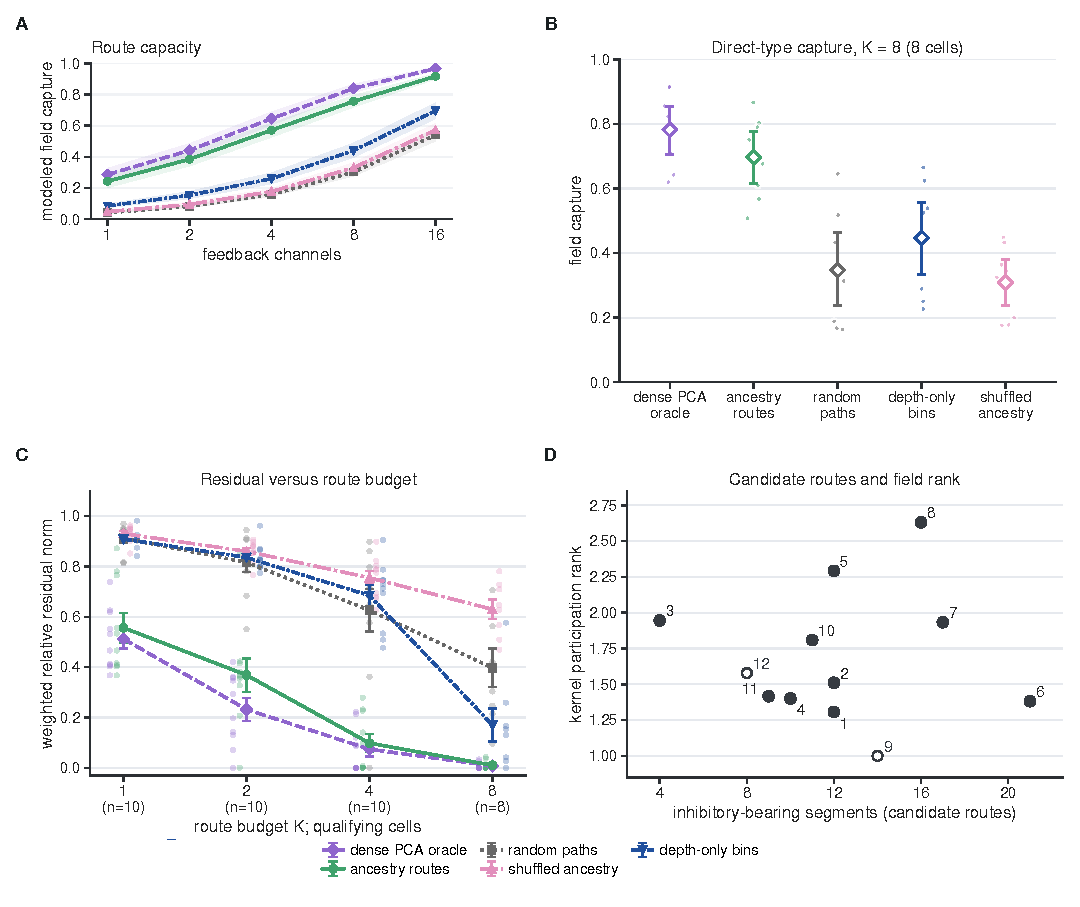
\includegraphics[width=\textwidth]{supplementary/curated/anatomy_capacity_controls.pdf}
\caption{\textbf{Cohort, label and arbor-size controls bound modeled anatomical capacity.} \textbf{A}, Route-generated field capture versus budget in 47 disjoint same-mouse cells; morphology routes use 8.1\% of dense-feedback wiring at eight channels. Twenty modeled streams are averaged within each cell; bands/bars are 95\% cell-bootstrap intervals. \textbf{B}, Initial eight-cell cohort: capture restricted to directly typed presynaptic contacts. \textbf{C,D}, Second-mouse Pinky cohort: relative residual norm versus route budget, and candidate-site count versus effective field rank. Eligibility changes from ten cells at $K\leq4$ to eight at $K=8$; small arbors approach the rank ceiling. Panel C uses mean $\pm$ s.e.m., and its residual norm is not squared-energy capture. All fields are model generated. Main Fig.~7 equalizes a common broadcast and leads with actual-tree surrogate controls; these route-generated comparisons are structural positive controls, not measured biological teaching signals.}
\label{fig:si_anatomy_capacity_controls}
\label{fig:supp_v661}
\label{fig:supp_morphology_detail}
\label{fig:supp_pinky}
\end{figure}

\begin{figure}[p]
\centering
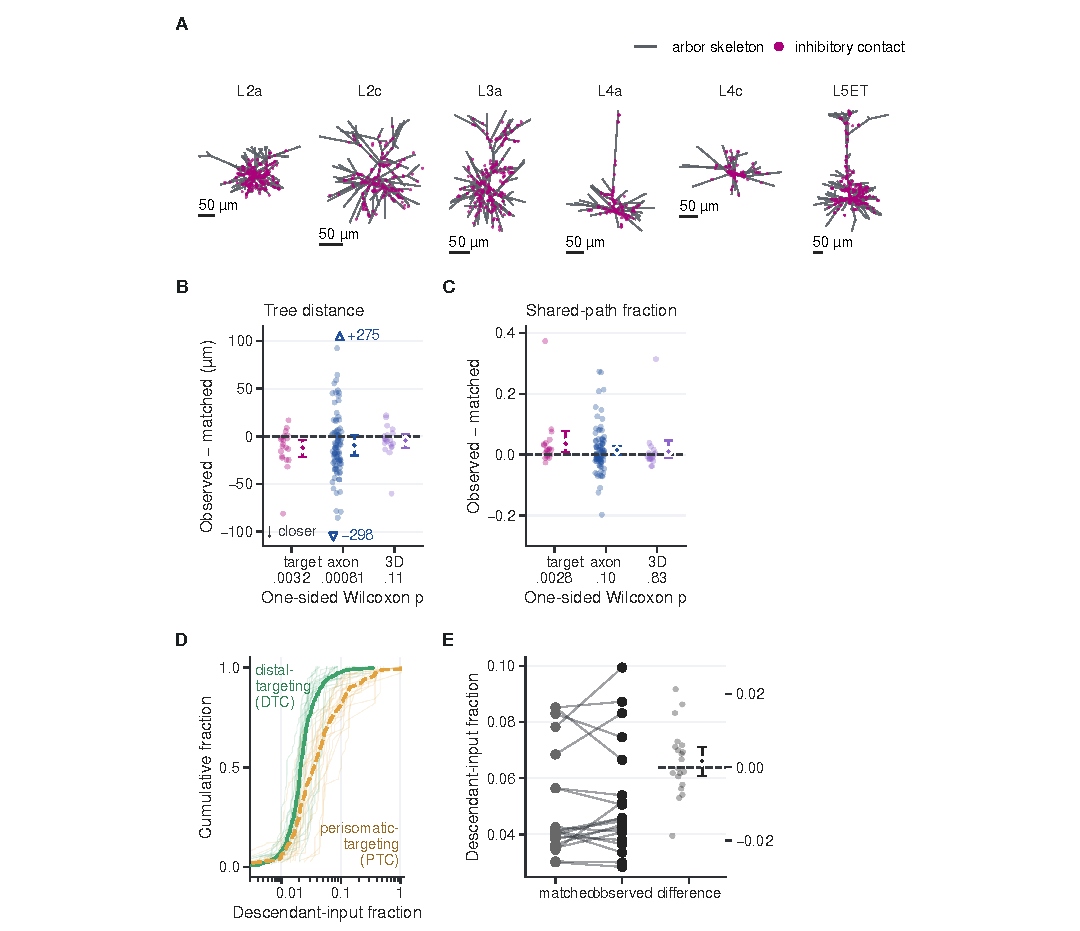
\includegraphics[width=\textwidth]{supplementary/curated/inhibitory_spatial_controls.pdf}
\caption{\textbf{Spatial matching limits apparent inhibitory targeting of ancestry domains.} \textbf{A}, Six layer-diverse reconstructions with mapped inhibitory contacts and physical scale bars. \textbf{B--D}, Observed-minus-matched tree distance, shared-path fraction and descendant-domain overlap in the twenty-target analysis, after aggregation within 92 presynaptic axons, and after joint path-distance/Euclidean matching. Symbols and intervals are means and 95\% bootstrap intervals over the displayed inferential unit. Only tree distance persists after axon aggregation; no endpoint persists after joint 3D matching. \textbf{E}, Descendant-input fraction by distal-dendrite- versus perisomatic-targeting class, retaining one contact per axonal clump. \textbf{F}, Inhibitory-contact domain size versus matched locations; no reliable overall localization advantage is detected. Cells derive from one mouse. These structural comparisons do not show that contacts carried teaching signals.}
\label{fig:si_inhibitory_spatial_controls}
\label{fig:supp_inhibitory}
\end{figure}

\begin{figure}[p]
\centering
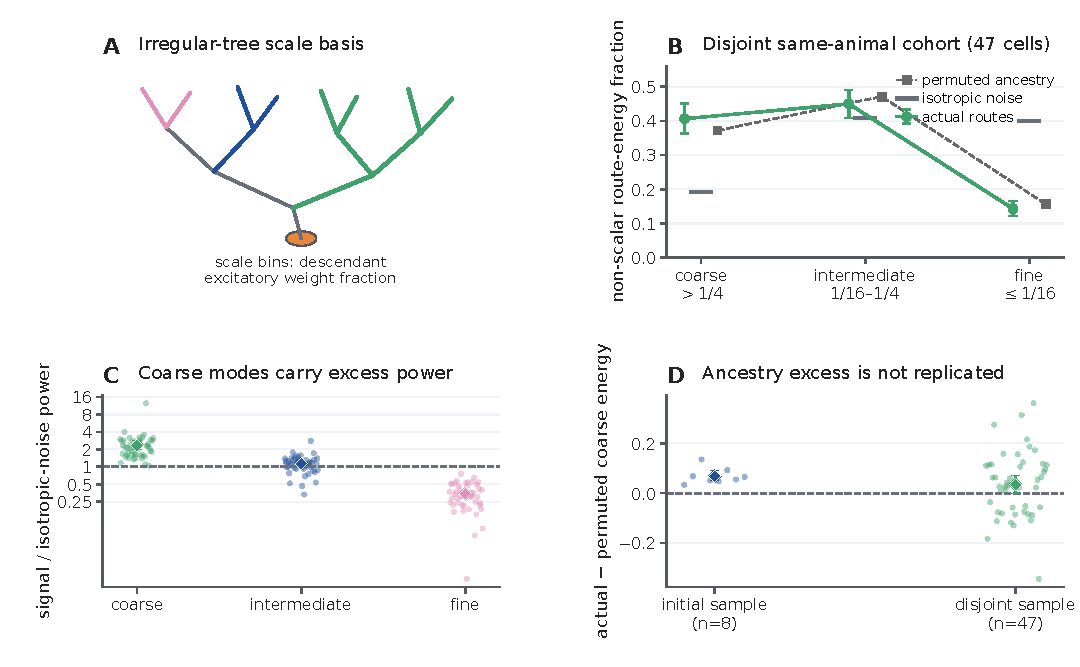
\includegraphics[width=\textwidth]{supplementary/curated/coarse_energy.pdf}
\caption{\textbf{Irregular reconstructed trees concentrate modeled route-field energy coarsely, but the anatomy-specific excess does not replicate.} \textbf{A}, Weighted unbalanced tree-Haar contrasts recursively partition each reconstructed arbor into coarse, intermediate and fine supports, defined by descendant excitatory-weight fractions \(>1/4\), \(1/16\)--\(1/4\) and \(\leq1/16\), respectively. \textbf{B}, Non-scalar conductance-weighted ancestry-route energy fraction in the disjoint 47-cell cohort, compared with column-permuted ancestry and dimension-matched isotropic noise. Actual-route points and intervals are cell means and 95\% cell-bootstrap intervals; null markers are cell means. \textbf{C}, Signal-to-isotropic-noise power by scale for all 47 cells; diamonds show means and 95\% cell-bootstrap intervals. \textbf{D}, Actual-minus-permuted coarse energy in the original and disjoint cohorts. The positive original-cohort contrast is not reliable in the 47-cell cohort. Cells are the inferential units; all reconstructions derive from one mouse. Modeled route fields are not measured teaching signals.}
\label{fig:si_coarse_energy}
\label{fig:supp_irregular_wavelets}
\end{figure}

\begin{figure}[p]
\centering
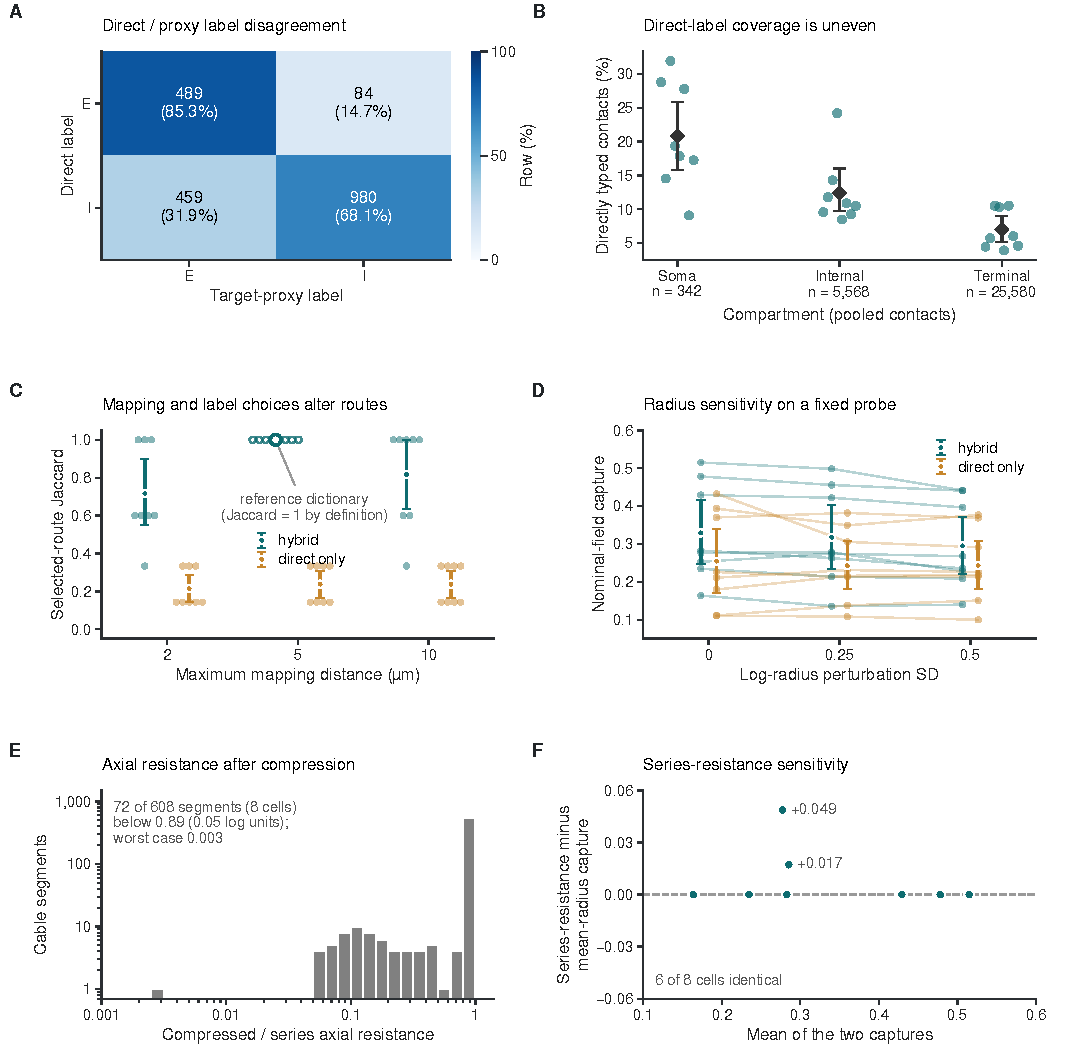
\includegraphics[width=\textwidth]{supplementary/curated/anatomy_preprocessing.pdf}
\caption{\textbf{Label coverage and geometric preprocessing affect anatomical route dictionaries.} All analyses use eight initial reconstructed cells from one mouse. \textbf{A}, Direct-presynaptic versus target-proxy excitatory/inhibitory (E/I) labels for 2,012 jointly labeled mapped contacts; counts and row percentages expose the asymmetric disagreement. Contacts are nested observations. \textbf{B}, Direct-label fraction by compartment: individual cells and cell means with 95\% cell-bootstrap intervals. Label availability is not assumed random. \textbf{C}, Jaccard overlap of the four selected routes with the nominal hybrid-label, $5\,\mu$m dictionary across mapping thresholds and label choices. \textbf{D}, Capture of the fixed nominal model-generated field under heterogeneous log-radius perturbations, indexed by their standard deviation (SD); five draws per nonzero dose are averaged within cell. Curves and bars in \textbf{C,D} show means and 95\% cell-bootstrap intervals (5,000 draws). \textbf{E}, Distribution of the mean-radius compressed axial resistance divided by the exact series sum over raw edges. Length preservation does not imply axial-resistance preservation. \textbf{F}, Paired cell capture under mean-radius and exact series-resistance normalizations, with leak terms held fixed. The diagonal marks equality. Across 1,056 retained sensitivity conditions, target fields, probe sites and weights remain those of the nominal model. These are preprocessing sensitivities, not calibrated geometric uncertainties or tests of endogenous task alignment.}
\label{fig:si_anatomy_preprocessing}
\label{fig:supp_morphology_uncertainty}
\end{figure}

\clearpage

% Curated from paper commit 7ee9157; original equations and protocol identities retained.
\section{Focal shunting and spatial transport}
\label{note:shunt_transport}

\subsection{Passive focal shunts attenuate a positive adjoint}

\begin{proposition}[No sign reversal in a passive grounded tree]
Let $G$ be a symmetric positive-definite nonsingular M-matrix, with
nonpositive off-diagonal entries. For a nonnegative adjoint source
$\bm s$, define $\bm q=G^{-1}\bm s$. Adding a
nonnegative shunt $\kappa$ at compartment $k$ gives
$G'=G+\kappa\bm e_k\bm e_k^{\mathsf T}$ and
\begin{equation}
\bm q'=\bm q-
\frac{\kappa q_k}{1+\kappa(G^{-1})_{kk}}G^{-1}\bm e_k.
\label{eq:s_sherman_shunt}
\end{equation}
Both $G^{-1}$ and $(G')^{-1}$ are elementwise nonnegative, hence
$0\leq\bm q'\leq\bm q$ componentwise. A focal passive shunt attenuates but
cannot reverse a positive adjoint field.
\end{proposition}

\noindent\emph{Proof.}
Equation~\ref{eq:s_sherman_shunt} is the Sherman--Morrison identity. A
nonsingular M-matrix has a nonnegative inverse; adding a nonnegative diagonal
term preserves the M-matrix property \citep{horn2013matrix}. The subtracted vector is nonnegative,
and $\bm q'=(G')^{-1}\bm s\geq0$. \hfill$\square$

This ordering does not by itself guarantee descendant selectivity relative to
a matched current injection; that spatial comparison depends on the Green's
function, focal site and electrotonic regime and is evaluated numerically in
the focal experiments.

\begin{corollary}[A focal shunt applies gains to its ancestry partition]
\label{cor:shunt_ancestry_gain}
Assume additionally that the nonzero off-diagonal entries of $G$ form a
connected tree rooted at the soma $s$, and that the adjoint source is
$\ell\bm e_s$ for a fixed scalar somatic loss derivative $\ell$. Write
$R=G^{-1}$ and $\bm h=R\bm e_s>0$. For a shunt at $k$, let
$\mathcal A_k$ be the vertices on the path from $s$ to $k$, including both
endpoints. For each $a\in\mathcal A_k$, define the disjoint block
$P_a=\{i:\operatorname{LCA}(i,k)=a\}$, where $\operatorname{LCA}$ is the
lowest common ancestor. Then
\begin{equation}
q'_i=\eta_a q_i\quad(i\in P_a),\qquad
\eta_a=1-\frac{\kappa R_{ks}R_{ak}}
{(1+\kappa R_{kk})R_{as}},\qquad
\eta_k=\frac{1}{1+\kappa R_{kk}}.
\label{eq:s_shunt_partition_gain}
\end{equation}
For finite $\kappa\geq0$, every gain satisfies $0<\eta_a\leq1$.
Let $B_k$ have columns $\bm 1_{P_a}$ and define the baseline-weighted
partition dictionary $D_k=\operatorname{diag}(\bm h)B_k$. With
$\Gamma_k=\operatorname{diag}(\eta_a)$,
\begin{equation}
\bm q=\ell D_k\bm 1,\qquad
\bm q'=\ell D_k\Gamma_k\bm 1.
\label{eq:s_shunt_partition_dictionary}
\end{equation}
Thus the adjoint effect is exactly a diagonal gain in this partition basis.
\end{corollary}

\noindent\emph{Proof.}
Removing a vertex $a$ separates a tree into components. If $a$ lies on the
path from $i$ to $j$, solving the source-free equations in the component
containing $i$, with boundary voltage at $a$, gives
$R_{ij}=R_{ia}R_{aj}/R_{aa}$. For
$a=\operatorname{LCA}(i,k)$, apply this identity to $(i,k)$ and $(i,s)$;
it also holds when an endpoint equals $a$. Hence
$R_{ik}/R_{is}=R_{ak}/R_{as}$. Substitution into
Eq.~\ref{eq:s_sherman_shunt} gives Eq.~\ref{eq:s_shunt_partition_gain}.
Positivity of both tree inverse matrices gives positive ratios, and the
preceding proposition bounds them by one. The formula also holds when
$\ell=0$, when both adjoints vanish. The disjoint blocks partition all
vertices, yielding Eq.~\ref{eq:s_shunt_partition_dictionary}.
\hfill$\square$

The block $P_k$ is the whole subtree below the shunt. For an ancestor $a$
above $k$, $P_a$ contains $a$ and its sister subtrees off the path to $k$.
If $c$ is the next vertex toward $k$, its indicator is
$\bm 1_{P_a}=\bm 1_{\mathrm{Desc}(a)}-\bm 1_{\mathrm{Desc}(c)}$,
whereas $\bm 1_{P_k}=\bm 1_{\mathrm{Desc}(k)}$. The gain field therefore
lies in the span of nested ancestry indicators. The diagonal form requires
the disjoint partition basis; an arbitrary selected set of overlapping
routes need not have diagonal gains. Even for the ancestry chain, a change
from partition to nested-subtree coordinates generally makes the gain
matrix non-diagonal, while preserving that full span.

For the synaptic gradient, the local driving force remains a separate factor:
$\gamma'_i=\eta_a q_i(E_{\mathrm E}-V'_i)$ for $i\in P_a$.
Its within-block variation is therefore not constrained to a single gain
relative to $\gamma_i=q_i(E_{\mathrm E}-V_i)$. The corollary describes
somatic-source adjoint transport on a passive tree, rather than the complete
synaptic update, a distributed-error source or a nonlinear finite-dose
response. It connects the morphology-defined dictionary to a conductance
gain without implying a learning advantage.

\begin{corollary}[Spectral size of a focal passive perturbation]
Under the preceding assumptions, let $\mathcal R=G^{-1}$ and
$\mathcal R'=(G+\kappa\bm e_k\bm e_k^{\mathsf T})^{-1}$. The inverse-operator change has
rank at most one, with rank one for $\kappa>0$, and
\begin{equation}
\lVert \mathcal R'-\mathcal R\rVert_2
=\frac{\kappa\lVert \mathcal R\bm e_k\rVert_2^2}
{1+\kappa \mathcal R_{kk}}
\leq
\frac{\kappa\lVert \mathcal R\rVert_2^2}
{1+\kappa/\lambda_{\max}(G)}.
\label{eq:s_focal_inverse_norm}
\end{equation}
Consequently, for any adjoint source $\bm s$,
$\lVert(\mathcal R'-\mathcal R)\bm s\rVert_2\leq
\lVert \mathcal R'-\mathcal R\rVert_2\lVert\bm s\rVert_2$.
\end{corollary}

\noindent\emph{Proof.}
Sherman--Morrison gives
$\mathcal R'-\mathcal R=-\kappa(\mathcal R\bm e_k)(\mathcal R\bm e_k)^{\mathsf T}/
(1+\kappa \mathcal R_{kk})$.
The norm of this symmetric outer-product matrix is its scalar coefficient times
$\lVert \mathcal R\bm e_k\rVert_2^2$. Use
$\lVert \mathcal R\bm e_k\rVert_2\leq\lVert \mathcal R\rVert_2$ and
$\mathcal R_{kk}\geq\lambda_{\min}(\mathcal R)=1/\lambda_{\max}(G)$ for the bound.
\hfill$\square$

Equation~\ref{eq:s_focal_inverse_norm} provides only a global magnitude ceiling
on the total adjoint change. It does not predict the localization contrast or
the observed crossover with membrane conductance. Those spatial effects depend
on the Green's-function profile and electrotonic length constant of the cable.

\subsection{Focal shunting perturbations}
\label{note:focal}

Route capacity does not show that conductance can selectively alter transport.
We therefore compared a focal shunt with a baseline-current-matched injection
at the same site of each reciprocal reconstructed cable and quantified the
resulting change in the exact modeled gradient.

\subsection{Adjoint formulation and baseline-current-matched current injection}

For passive conductance matrix $G$ and current-source vector $\bm b$, the
voltage vector was $\bm V=G^{-1}\bm b$. Let $\bm e_s$ select the somatic
coordinate and let $w_i$ denote the excitatory conductance at site $i$. For a
loss depending on somatic voltage, the adjoint error and conductance gradient
were
\begin{equation}
\bm q=G^{-1}\bm e_s\frac{\partial\mathcal L}{\partial V_s},
\qquad
\frac{\partial\mathcal L}{\partial w_i}=q_i(E_{\mathrm E}-V_i).
\end{equation}
Adding focal inhibitory conductance \(\kappa_k\) at node $k$, selected by
the coordinate vector $\bm e_k$, gives
\[
G'=G+\kappa_k\bm e_k\bm e_k^{\mathsf T},
\qquad
\bm b'=\bm b+\kappa_kE_{\mathrm I}\bm e_k .
\]
The shunt therefore changes both conductance loading and the forward source.
Holding the somatic loss derivative fixed, the Sherman--Morrison identity
gives the transport change
\begin{equation}
\bm q'=\bm q-
\frac{\kappa_kq_k}{1+\kappa_k(G^{-1})_{kk}}G^{-1}\bm e_k.
\label{eq:s_sherman}
\end{equation}
The reversal \(E_{\mathrm I}\) does not appear in
Eq.~\ref{eq:s_sherman} because the adjoint transport depends on \(G'\), not on
the forward source \(\bm b'\). It remains in the solved voltage and in every
inhibitory driving force.
Corollary~\ref{cor:shunt_ancestry_gain} supplies the exact partition-gain form. The full synaptic gradient additionally changes through its local driving force.

Let $r_k=(G^{-1})_{kk}>0$. Then
\begin{equation}
\Delta\bm q=-a_kG^{-1}\bm e_k,
\qquad
a_k=\frac{\kappa_kq_k}{1+\kappa_kr_k},
\qquad
\frac{\partial |a_k|}{\partial\kappa_k}
=\frac{|q_k|}{(1+\kappa_kr_k)^2}\geq0.
\label{eq:s_shunt_amplitude}
\end{equation}
The derivative is strictly positive when $q_k\neq0$; if $q_k=0$, the perturbation vanishes. Its amplitude saturates at $|q_k|/r_k$. For a nonzero perturbation, the normalized spatial profile is fixed by the Green's-function column $G^{-1}\bm e_k$ in this linear passive state. For a
descendant set $D(k)$ and a prespecified matched comparison set $C(k)$, define
\begin{equation}
S_k(D,C)=
\frac{\operatorname{median}_{i\in D(k)}|(G^{-1})_{ik}|}
{\operatorname{median}_{j\in C(k)}|(G^{-1})_{jk}|}.
\label{eq:s_electrotonic_selectivity}
\end{equation}
For $\kappa_k>0$, $q_k\neq0$ and a positive comparison median, the common amplitude $|a_k|$ cancels. Under these conditions, $S_k>1$ is necessary and sufficient for a positive descendant-minus-comparison contrast in absolute adjoint change at fixed $k$. It is only a transport-level criterion. Relative
or logarithmic changes additionally divide by the baseline $q_i$, and the full
synaptic gradient also contains the post-perturbation driving force. This is
why axial coupling, leak, background conductance and local input resistance
must be varied explicitly rather than inferred from topology alone.
The baseline-current-matched current injection applied
$\kappa_k(E_{\mathrm I}-V_k)$ at the same node without changing $G$. This equals the
current carried by the added shunt at the unperturbed voltage; its local
voltage effect matches the shunt only to first order in dose. An independently
solved state-matching compensatory current injection restored baseline somatic
voltage after both interventions. This is not a continuously adjusted voltage
clamp. The somatic scalar error was therefore fixed. Shunting changed adjoint
transport, whereas the current-injection control left it unchanged. Dendritic voltages
were not clamped, so both interventions could also change local driving forces.

\subsection{Prespecified endpoint and numerical validation}

Before running the analysis, we fixed the site-selection rule, primary dose,
comparison groups, and localization endpoint. Focal sites were selected by a
depth-stratified rule without access to gradient outcomes. A site required at
least three excitatory descendants and
three comparison sites. At most 16 eligible sites were sampled per cell across
quartiles of topological depth. The primary model used excitatory and
inhibitory synaptic scales of 0.35 and normalized reversal potentials
$E_{\mathrm E}=1$ and $E_{\mathrm I}=-0.2$. Synapses were classified as descendants, ancestors,
sister-subtree sites or unrelated sites. Unrelated synapses within each
template were matched to descendant cable depth. For baseline gradient $g_i$
and perturbed gradient $g_i'$, we defined
$m_i=\left|\log[(|g_i'|+\varepsilon)/(|g_i|+\varepsilon)]\right|$, where
$\varepsilon=10^{-15}\max(1,\max_i|g_i|)$. For each site, the localization
index was the median $m_i$ among descendants minus the median among
depth-matched unrelated synapses. Site effects were first averaged within cell.

The somatic loss was one-half the squared difference between somatic voltage
and a target one normalized unit below its baseline value. Conductance doses
were 0.25, 0.5, 1, and 2 times the local leak-plus-synaptic conductance. The
state-matching current was solved after each perturbation and then treated as
fixed when evaluating the post-intervention conductance gradient. The topology
control sampled 200 relation templates from other focal sites, stratified by
focal-site topological-depth quartile when another site was available;
otherwise it sampled another site in the same cell.

At unit dose, 101 sites in eight cells gave mean localization 0.104 for shunting and 0.035 for current injection. Their paired cell-level contrast was 0.069 log units (95\% interval, 0.053--0.086), positive in all eight cells. True relations also exceeded the depth-stratified relation control. The contrast grew with relative dose; Source Data retain every site, dose and template.

We separated the two factors in the exact gradient algebraically. Writing
$d_i=E_{\mathrm E}-V_i$ and $d'_i=E_{\mathrm E}-V'_i$, full shunting uses $q'_id'_i$,
adjoint-only substitution uses $q'_id_i$, and driving-force-only substitution
uses $q_id'_i$. At unit dose, their mean localization indices were 0.104,
0.130 and 0.026, respectively, compared with 0.035 for the current-injection
control. Adjoint-only minus driving-force-only localization was 0.104 (95\%
interval 0.080--0.125), positive in all eight cells.

Full shunting and the driving-force-only state provide a direct comparison
of adjoint transport: they share the same post-shunt voltage field and differ
only in whether the adjoint field is updated. Their localization difference was 0.079 and was positive in all
eight cells. This is the exact adjoint-replacement contrast plotted in main
Fig.~8C.

The gradient factors and localization statistic are nonlinear, so these four
outcomes do not form an additive decomposition. To allocate the
full-shunt-minus-current-injection contrast, we used two-factor Shapley values.
For $v_{00}$ equal to current-injection localization, $v_{10}$ adjoint-only,
$v_{01}$ driving-force-only and $v_{11}$ full-shunt localization,
\begin{align}
\phi_q&=\tfrac12[(v_{10}-v_{00})+(v_{11}-v_{01})],\\
\phi_d&=\tfrac12[(v_{01}-v_{00})+(v_{11}-v_{10})].
\end{align}
The allocations sum exactly to the full-shunt-minus-current contrast. Mean adjoint and driving-force allocations were 0.087 and $-0.017$, respectively: driving-force change partly cancelled the adjoint contribution. This is an algebraic allocation of a nonlinear statistic; the current-matched control is not a literal no-factor corner of a physical factorial. Repeating the allocation with the unperturbed field as its reference is retained in Source Data. Factor substitutions are not independent biological interventions.

All conductance matrices in the primary analysis were positive definite. The
somatic state-matching residual was numerically zero. Analytic adjoint gradients agreed
with finite differences to a maximum relative error of
$1.03\times10^{-6}$. The Source Data indexed in Table~\ref{tab:source_index} retain prespecified
conductance-scale and reversal-potential sensitivity runs. The direction of
the shunting-minus-current-injection effect was positive in every condition,
with seven or eight positive cells. These results establish the mechanism in a passive model on measured trees;
they do not establish endogenous inhibitory teaching signals in vivo.

With proxy-classified contacts removed, the primary
shunt-minus-current-injection contrast was 0.101 (0.075--0.129) across 55 sites
and was positive in all eight cells. In the independent, non-overlapping v661
sample, 45 cells supplied 235 eligible sites. The same contrast was 0.138
(0.116--0.162), positive in 45/45 cells. Forty cells
with at least two eligible sites supplied the reassigned-relation control; the
true relation exceeded this control by 0.118 (0.094--0.144), with
39 positive cells and one numerical tie (Supplementary
Fig.~\ref{fig:si_shunt_replication}A,B). Cells, rather than
sites or relation draws, were the
units of inference.

To test sensitivity to electrical calibration, we also computed axial and
leak conductances in physical units from the same compressed geometry. For
segment radius $r$, length $\ell$, axial resistivity $R_a$ and specific
membrane resistance $R_m$, a cylindrical non-root segment had axial conductance
$\pi r^2/(R_a\ell)$ and membrane leak $2\pi r\ell/R_m$; the root was assigned
spherical area $4\pi r^2$. All conductances were converted to nanosiemens (nS). Because MICrONS
synapse size is not an electrical conductance, synaptic sizes retained the
prespecified relative scaling with the median physical leak as reference. We
varied $R_a$ and $R_m$ while retaining the site-selection rule, relative dose, gradient definition and current-injection control. For each condition and intervention, we re-solved the compensating somatic current to restore that condition's baseline somatic voltage. The Source Data indexed in Table~\ref{tab:source_index} retain this electrotonic dependence. The large contrast observed under the normalized proxy was recovered only in
low-$R_m$, high-conductance settings; at
$R_a=150\,\Omega\,\mathrm{cm}$ and
$R_m=15{,}000\,\Omega\,\mathrm{cm}^2$ it was negligible or small. These are
sensitivity settings, not fits to the recorded cells, and the model remains
passive and steady-state.

A broader parameter matrix, specified before numerical validation, tested
membrane resistance, background conductance and dose definition jointly. It used
\(R_a=150\,\Omega\,\mathrm{cm}\) and crossed
\(R_m\in\{300,1000,15{,}000\}\,\Omega\,\mathrm{cm}^2\), distributed leak-like
background conductance of 0, 1 or 4 times baseline leak, and three dose
definitions. Relative-local doses were 0.25, 1 and 2 times membrane-plus-
synaptic conductance; fixed doses were 0.05, 0.5 and 5 nS; input-normalized
doses were 0.25, 1 and 4 times $[(G^{-1})_{kk}]^{-1}$. The same 101 sites in
eight cells supplied 16,362 site--condition--intervention rows. Every
conductance matrix was positive definite (minimum eigenvalue 0.107 nS) and the
maximum somatic-state residual was $3.33\times10^{-16}$.

At fixed absolute dose, the conductance-specific contrast did not follow the
raw focal-shunt localization alone. At 0.5 nS, shunt-minus-current-injection
localization was 0.0104 (0.0080--0.0126), 0.0073 (0.0044--0.0104), and
$-0.0039$ ($-0.0075$ to $-0.0004$) at $R_m=300$, 1,000 and 15,000,
respectively. At 5 nS the corresponding values were 0.0974, 0.0741 and 0.0061;
the last interval included zero. Distributed background conductance restored
the input-normalized effect in the high-resistance condition: at unit
input-conductance dose, the contrast changed from $-0.0004$ with no background
to 0.1210 and 0.2587 at background multipliers one and four. Across all 8,181
focal-shunt rows, every descendant gradient magnitude was attenuated, none was
enhanced and no sign flip occurred. The passive mechanism therefore selectively attenuated gradients; sign
reversal would require dynamics or active conductances absent from this phase (Supplementary Fig.~\ref{fig:si_shunt_sensitivity}).

\subsection{Weak-channel steady-state linearization check}

We checked the local-Jacobian calculation after adding weak
voltage-dependent currents to the high-conductance cable.
The physical reconstructed-tree system used
$R_a=150\,\Omega\,\mathrm{cm}$,
$R_m=1{,}000\,\Omega\,\mathrm{cm}^2$ and distributed background conductance
equal to baseline leak. Steady-state sodium (Na), potassium (K), calcium (Ca),
hyperpolarization-activated cyclic nucleotide-gated (HCN) and
N-methyl-D-aspartate receptor (NMDA) current families had fixed reversal
potentials, half-activation voltages, slopes and gate
powers specified in the predefined parameter file. Global and segment-level
maximal conductances were drawn independently from prespecified log-normal
distributions. Median maximal Na, K, Ca and HCN conductances were 0.06,
0.10, 0.025 and 0.05 times baseline leak, respectively; NMDA conductance was
0.15 times the excitatory conductance. Gate activation further scales these
currents. These prespecified weak-channel draws are not cell-specific
density estimates or a test of strongly regenerative operation.

For each draw, a residual-reducing Newton solve found the nonlinear steady
state. The predefined acceptance criteria required all voltages to lie in the
specified range, maximum absolute state residual below $10^{-10}$, and minimum
eigenvalue of the symmetrized local Jacobian above $10^{-8}$. The implicit-adjoint calculation
then used the exact inverse of this baseline Jacobian. For channel family $a$, let $\bar g_a$ be maximal conductance, $h_a(V)$ the
steady-state gating factor and $E_a$ the reversal potential. The current
$I_a(V)=\bar g_a h_a(V)(V-E_a)$ contributed the diagonal term
$\bar g_a[h_a(V)+h_a'(V)(V-E_a)]$; thus the baseline Jacobian includes
voltage-dependent gate derivatives. Focal shunting and a
baseline-current-matched current injection were evaluated at 0.25, 1 and 4
times local input conductance within this fixed local linearization.
Sherman--Morrison updated the Jacobian inverse for the added focal
conductance, and a compensating somatic current restored baseline somatic
voltage in that linearized system. The active gates and their derivatives
were not re-evaluated at a new nonlinear equilibrium after each finite dose.
Up to 256 attempts were permitted to obtain 64
accepted draws per cell. All first 64 attempts were accepted in every cell,
giving 512 equilibria, 101 focal sites and 38,784 site--draw--condition rows.
All values were finite, the largest equilibrium residual was
$9.51\times10^{-11}$ and the smallest Jacobian eigenvalue was 1.084.

Channel draws and focal sites were averaged within each of the eight cells
before inference. At doses 0.25, 1 and 4, mean shunt localization was 0.159,
0.529 and 1.339, respectively (Table~\ref{tab:source_index}). At unit dose,
shunting exceeded the current-injection control by 0.382 (95\% cell-bootstrap
interval 0.356--0.409), positive in 8/8 cells (two-sided Wilcoxon $P=0.0078$).
Every modeled descendant gradient was attenuated, none was enhanced or changed
sign, and descendant gradient energy fell to 0.330 of baseline. The dose
response closely followed the passive response at the same electrical
calibration. This agreement checks the weak-channel linearization; it does
not establish robustness to strongly active dendrites, channel kinetics or
spiking.

\subsection{Driving-force cancellation and the ancestry dependence of passive fields}
\label{sec:passive_field_diagnostics}
We reanalyzed the eight original cable operators used for the common-broadcast comparison. For each focal site, the perturbation was the original dose 0.001 with somatic voltage restored. The finite log-gradient difference divided by dose separates into an adjoint term and a driving-force term. Energy uses the original excitatory-area site weights and sums over focal perturbations. The full focal ancestry partition is defined separately for each shunt and is distinct from the seven selected routes in the budgeted anatomical dictionary.

Driving-force energy was 0.990--3.496 times full-field energy across cells; these are ratios of squared magnitudes, not amplitudes. Weighted centered correlations with the adjoint term were $-0.979$ to $-0.913$. The negative cross term explains why large components yield a smaller full response. The full response retained 0.9711--0.9993 of its energy in the focal partition. Reconstruction agrees with the original operators to $10^{-8}$; numerical decomposition closes to rounding error. Cellwise energies, correlations and partition captures are supplied in Source Data.

The passive corollary depends on a tree Green's function, a somatic adjoint source and a diagonal conductance change. Choosing other passive perturbations under the same assumptions does not make the anatomical field ancestry-neutral. The budgeted dictionary comparison measures compression within this response family. In the disjoint 47-cell cohort, actual ancestry exceeds the mean degree--depth surrogate in 38 cells, but in eleven cells more than half of 200 surrogates match or exceed the actual tree. This descriptive count uses tolerance $10^{-12}$ and retains the full within-cell distribution. A different error source, active dynamics or measured fields would be required to test beyond the present structural dependence.

\begin{figure}[p]
\centering
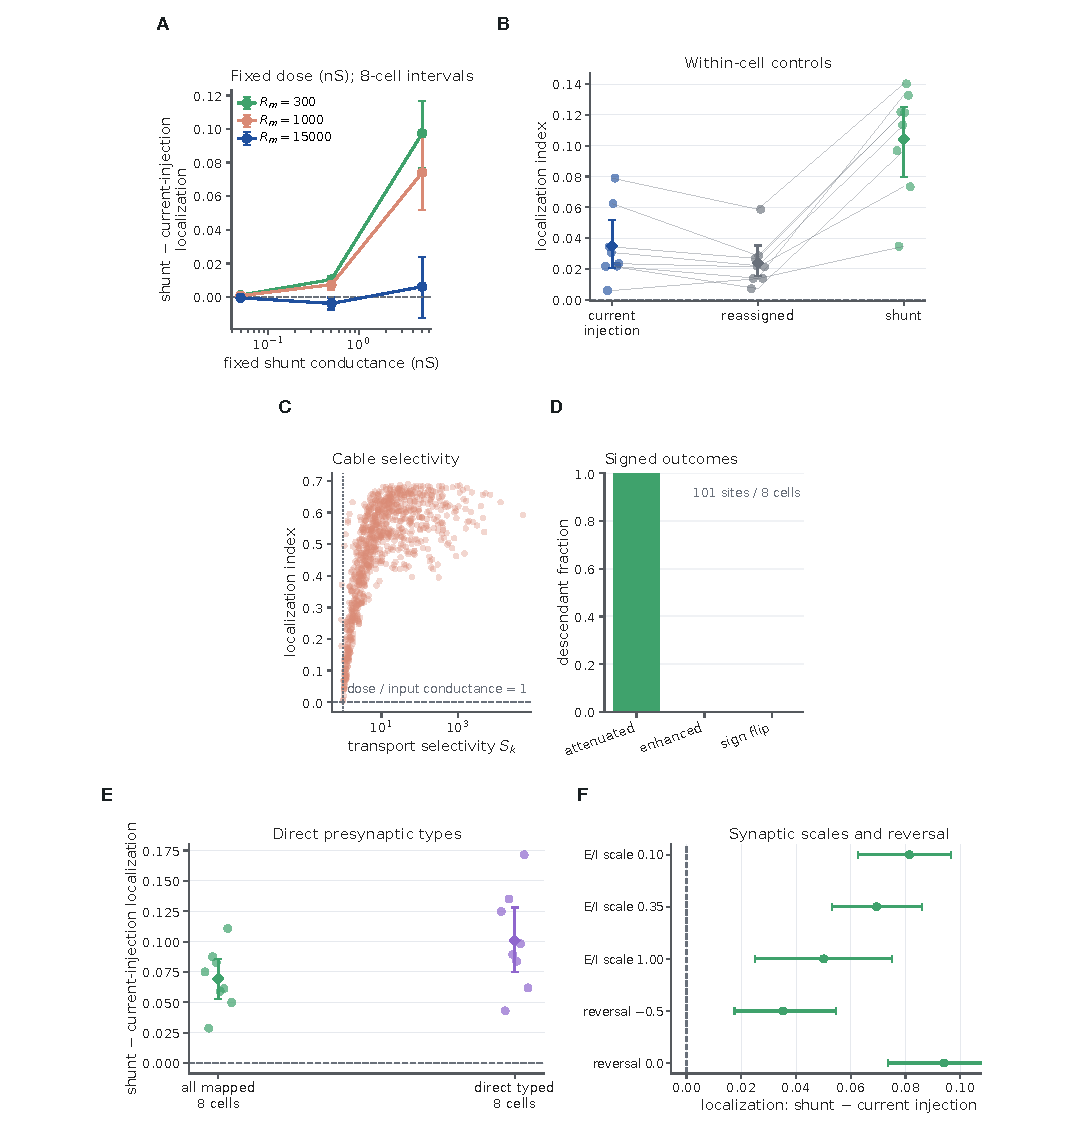
\includegraphics[width=\textwidth]{supplementary/curated/shunt_sensitivity.pdf}
\caption{\textbf{Dose, cable parameters and input mapping determine focal-shunt selectivity.} \textbf{A}, Shunt-minus-current-injection localization across fixed absolute doses at three membrane resistances ($R_m$ of 300, 1,000 and 15,000~$\Omega\,\mathrm{cm}^2$: one lightness step, marker and dash pattern each) and three background-conductance multipliers (column groups), on a symmetric-log axis that is linear within $\pm0.001$. The contrast is close to proportional to dose at every setting, and the $R_m$ ordering reverses with background: with no background the $R_m=15{,}000$ contrast stays near zero (slightly negative at 0.05 and 0.5~nS, an interval spanning zero at 5~nS), whereas at background multiplier four it is the largest of the three at every dose, with 8/8 cells positive. \textbf{B}, Shunt and matched-injection localization (grey lines pair cells) and the true relation against a reassigned foreign template (unpaired); positive favors the shunt or the true relation. \textbf{C}, Transport selectivity $S_k$ against full synaptic-gradient localization at unit input-conductance-normalized dose, 101 sites; descriptive site--regime points, $R_m$ colours as in \textbf{A}, background multipliers 0, 1 and 4 as filled, open and plus markers; dotted line, $S_k=1$. \textbf{D}, Signed census of the same sites at $R_m=1{,}000\,\Omega\,\mathrm{cm}^2$, background multiplier one, unit dose: fraction of descendant gradients attenuated, enhanced or sign reversed by shunt (attenuates only) and matched injection (enhances only), as in all 81 passive conditions. \textbf{E}, All mapped versus directly typed contacts (grey lines pair cells); the contrast increases in 8/8 cells. \textbf{F}, E/I scale and inhibitory-reversal sensitivity by row; open marker and band, the reference condition (E/I 0.35, reversal $-0.2$) and its interval; right column, cells with a positive contrast. \textbf{A,B,E,F}, means and 95\% cell-bootstrap intervals, eight cells.}
\label{fig:si_shunt_sensitivity}
\label{fig:supp_focal_matrix}
\label{fig:supp_focal_detail}
\end{figure}

\begin{figure}[p]
\centering
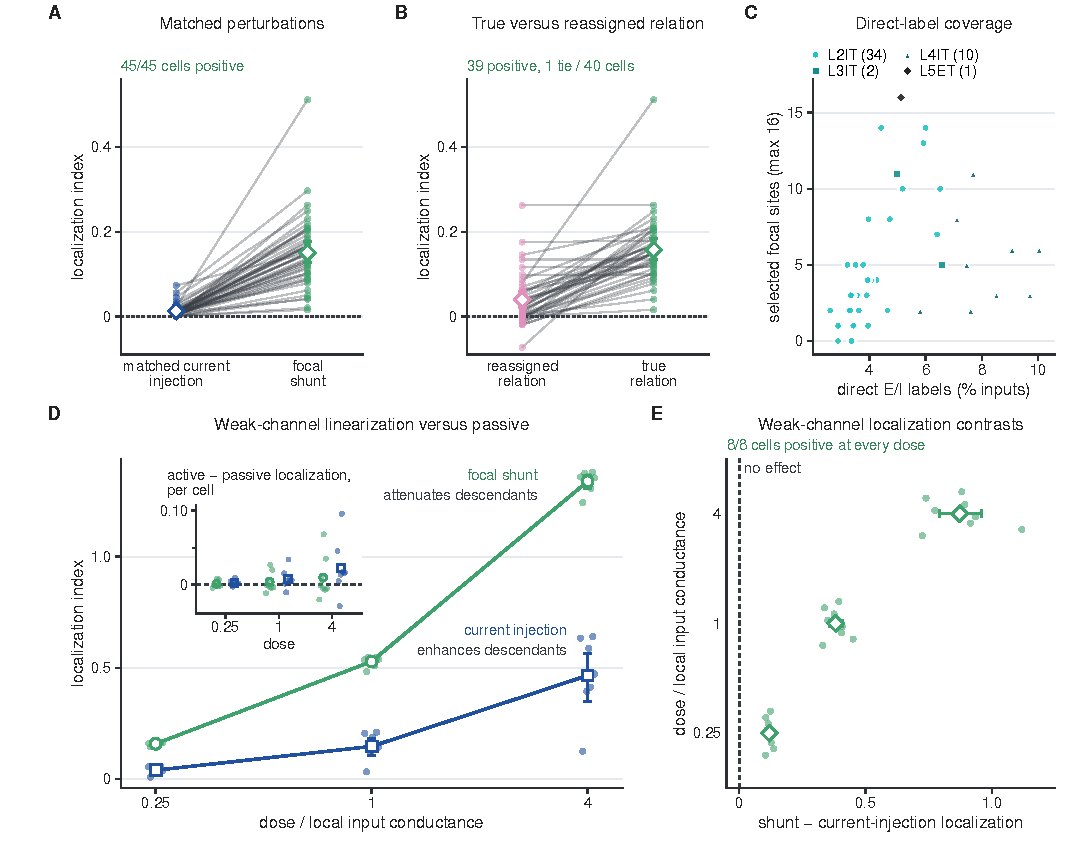
\includegraphics[width=\textwidth]{supplementary/curated/shunt_replication.pdf}
\caption{\textbf{Focal-shunt controls replicate structurally and under weak-channel linearization.} \textbf{A}, Focal shunt versus baseline-current-matched injection in 45 disjoint same-mouse cells (235 sites). \textbf{B}, True versus reassigned descendant relation templates in forty cells (230 sites); the true-relation column repeats the focal-shunt values of \textbf{A} for the forty cells that have a reassigned-relation partner. \textbf{C}, Direct E/I label coverage and the number of selected focal sites per cell, capped at 16 (one L5ET cell had 47 eligible sites); cell classes are ordinal colours within this panel. \textbf{D,E}, Separate initial eight-cell weak-channel ensemble: localization versus dose (dose divided by local input conductance) and paired shunt-minus-current contrasts. A fixed steady-state Jacobian (solid) is compared with the passive model (dashed); the two means differ by at most 0.010 localization units for the shunt and 0.023 for current injection at every dose, so the passive curve lies under the active one. Shunting attenuates descendants whereas matched current injection enhances them. Sixty-four channel draws and sites are averaged within each cell; intervals bootstrap cells and are narrower than the marker except at dose 4, and the contrast is positive in 8/8 cells at every dose (Wilcoxon $p=0.0078$). Weak conductances test local linearization near the passive response and do not establish robustness to regenerative dynamics or channel kinetics.}
\label{fig:si_shunt_replication}
\label{fig:supp_weak_channel_linearization}
\end{figure}

\clearpage

% Curated from paper commit 7ee9157; original equations and protocol identities retained.
\section{Measured responses, model diagnostics and detection sensitivity}
\label{note:measured_responses}

\subsection{Functional topology and task-derived credit}
\label{note:functional}

Anatomical routes can be available without aligning with the credit required
by a measured task. We therefore used recorded visual responses to define a
prediction objective on reconstructed target cells. Within each model, we
changed the backward field while holding the forward morphology fixed.

\subsection{Direct anatomy--function join}

Functionally imaged excitatory partners were linked to anatomical contacts
through MICrONS/CAVE and DANDI mappings. The analysis contained 69 connected
presynaptic partners across seven postsynaptic target cells. Automatic
matches came from
\texttt{coregistration\_auto\_phase3\_fwd\_apl\_vess\_combined\_v2} in
materialization 1822. We retained residual at most 10 and score at least zero,
then deduplicated each presynaptic root by ascending residual and descending
score. All mapped contacts from a retained presynaptic root contributed to its
partner-level contact summary. For the one-site-per-partner model, contacts
were first grouped by postsynaptic segment. The partner was assigned to the
segment with greatest summed contact size, breaking ties by synapse count, and
its major branch was the first segment below the soma on that segment's
ancestry chain. Thus a partner with contacts on several segments supplied one
activity feature and one modeled learning site; its total contact size and
synapse count still included all retained contacts.

The target universe was the initial eight-cell morphology convenience sample.
The analysis plan, specified before outcome inspection, included every target
in that sample with a DANDI scan and directly connected, functionally imaged
excitatory partners; seven targets qualified. Predefined inclusion criteria
required exactly one postsynaptic target in an
extract, agreement between partner and contact counts, at least five mapped
partners for the topology screen, at least two sites after any requested task
filter, and at least one nonempty inhibitory nested-subtree route. The primary
task analysis applied neither a manual-match restriction nor a repeat-reliability
threshold. The exact target/session/scan pairs are retained in the source records indexed in Table~\ref{tab:source_index}. The original analysis plan did not record a
deterministic rule for choosing among multiple eligible scans of the same
target. We therefore treat these scan choices as part of the initial
selected-scan sample, not as the output of a coverage-ranking procedure.
The omitted structural target, root 864691136043380566 (nucleus 292648), had
one source-data row, for session 8/scan 4, but
\texttt{has\_dandi\_asset=False} and no DANDI asset identifier or path. No
additional exclusion reason is inferred.

A deterministic sensitivity retained every automatic-conservative target--session--scan cohort with at least five imaged connected presynaptic roots: thirteen scans across the same seven targets. Statistics were computed within scan, averaged within target and inferred over targets. The mean partial shared-path correlation was $-0.0485$ (95\% target-bootstrap interval, $-0.224$ to 0.118), positive in three targets. The selected-scan and scan-complete analyses therefore both provide no evidence of preferential ancestry alignment. Full topology endpoints are indexed in Supplementary Table~\ref{tab:source_index}.

Each target had 464 trials and 280 unique condition hashes, of which 136 were
repeated. Trial families comprised 384 Clip, 40 Monet2 and 40 Trippy
presentations. For each trial and region of interest, the response was the
mean of the supplied \texttt{RoiResponseSeries} fluorescence trace over samples whose timestamps
fell from trial start through trial stop, including both endpoints. Start and
stop offsets were zero. These are the supplied fluorescence traces; our analysis did not deconvolve or apply additional raw-fluorescence preprocessing to them. No trials were dropped; every response used here was
finite. The records indexed in Table~\ref{tab:source_index} give target-level asset identifiers
and sample counts.

Functional similarity between two partners was the Pearson correlation of
their vectors of condition-mean fluorescence over the 136 condition identities with
at least two trials. Repeat reliability was computed separately for each
region of interest: successive occurrences of every repeated condition were assigned alternately
to two groups, responses were averaged within each group,
and the two vectors of condition means were compared by Spearman correlation.
No reliability correction was applied, and the primary cohort retained all
partners regardless of this diagnostic; thresholds of 0.1 and 0.2 were used
only in sensitivity analyses.

The controlled shared-ancestry statistic was computed separately within each
target. Functional similarity and shared-path fraction were rank transformed.
The two controls were $\log(1+d_{\mathrm{Euclidean}})$ and
$\log(1+|d_{\mathrm{soma},i}-d_{\mathrm{soma},j}|)$, where the second term is
the absolute difference in soma path length; each control was also rank
transformed. We regressed each ranked variable on an intercept and the two
ranked controls by ordinary least squares, then took the Pearson correlation
between the two residual vectors. The mean target-level partial-rank effect
was $-0.069$ with a target-bootstrap 95\% interval of $-0.251$ to 0.106;
three of seven targets had positive effects. Pairwise partner comparisons were
not treated as independent replicates.

Several features limit the interpretation of this cohort. MICrONS calcium
imaging measured excitatory neurons, the observed partners cover only a small
fraction of each target's complete inputs, and response reliability is modest.
The volume comes from one animal, and the recordings were not made during
learning.

\subsection{Task-derived branch credit}

A branch model predicted the standardized postsynaptic response from the
standardized responses of its connected presynaptic partners. Let $x_i$ be the
response of partner/site $i$, $w_i$ its input weight, and $b(i)$ the dominant
major branch receiving its contacts. Branch $b$ had summed input $d_b$,
activity $h_b$ and readout weight $v_b$; $c$ was an output bias. The fitted
prediction $\widehat y$ was
\begin{align}
d_b&=\sum_{i:b(i)=b}x_iw_i,
&h_b&=\tanh(d_b),
&\widehat y&=\sum_bv_bh_b+c.
\label{eq:s_branch_model}
\end{align}
For $N$ training trials with target responses $y_t$, the objective was
\begin{equation}
\frac{1}{2N}\sum_{t=1}^{N}(\widehat y_t-y_t)^2+
\frac{\lambda}{2}(\lVert\bm w\rVert_2^2+\lVert\bm v\rVert_2^2),
\qquad \lambda=10^{-3},
\label{eq:s_branch_objective}
\end{equation}
with no penalty on $c$. The exact voltage-space error at site $i$ was
$(\widehat y-y)v_{b(i)}[1-\tanh^2(d_{b(i)})]$.

Whole condition-hash stimulus identities, not trials of the same identity,
were split: 20\% of the 280 identities and all of their trials were held out.
Input columns and the target were standardized separately using training-set
means and sample standard deviations ($\mathrm{ddof}=1$); invalid or zero
scales were replaced by one and remaining nonfinite standardized values by
zero. A stable \texttt{SeedSequence} combined base seed 20260721, target root,
stream and replicate. There were ten fixed split and initialization replicates
per target.

With $n_{\mathrm{site}}$ input sites and $n_{\mathrm{branch}}$ occupied
branches, input weights were initialized as
$\mathcal N(0,0.12^2/n_{\mathrm{site}})$, branch readout weights as
$\mathcal N(0,0.25^2/n_{\mathrm{branch}})$, and $c=0$. Each method used
1,200 full-batch Adam steps with learning rate 0.015,
$(\beta_1,\beta_2)=(0.9,0.999)$ and $\epsilon=10^{-8}$. The exact model was
trained first. Its exact site-error fields on training trials defined the
dictionaries and its held-out exact field defined reported capture. All
projected-learning methods then restarted from the identical initial state.
Only the input-weight error was projected; $\bm v$ and $c$ always received
their exact gradients.

The primary budget requested four channels, reduced only when a target had
fewer sites or nonempty candidate routes. Ancestry candidates were columns
of ancestry multiplied by local inhibitory fraction $g_i/g_{\mathrm{tot}}$;
routes were ranked by this fraction times their descendant-site fraction.
Random paths sampled nonempty candidates uniformly without replacement.
Each ancestry-shuffle column was permuted independently over sites. Depth
controls were path-length quantile bins, scalar feedback was an all-ones
column, and the dense oracle used the leading right singular vectors of the
exact training error. Projectors used relative singular-value tolerance
$10^{-10}$. No held-out response was used to fit a dictionary.

Held-out normalized MSE divided a method's held-out MSE by the MSE of
predicting the training mean response. Replicates were averaged within target
before inference; the seven target cells were the units. Intervals used 20,000
target bootstrap draws. Paired method comparisons used two-sided Wilcoxon
tests, and the capture--utility analysis used method-label permutations
stratified within target.

The four-channel primary outcomes are retained in the Source Data indexed in Table~\ref{tab:source_index}.
The dense four-dimensional oracle nearly matched exact learning, establishing
that feedback dimension alone was not limiting in this surrogate. Ancestry routes
did not reliably outperform ancestry shuffling in capture or learning. The
within-target association between capture and normalized error was
$\rho=-0.150$ with a target-stratified method-label permutation $P=0.419$.
The target-bootstrap 95\% interval for $\rho$ was $-0.449$ to 0.144. The coefficients are
least-squares oracles and therefore upper bounds on the capacity of each
feedback family, not biologically implemented encoders.

Sensitivity analyses at one, two and eight channels, with direct manual
matches, with repeat-reliability thresholds, and with a linear branch model
did not establish a reliable morphology-specific learning benefit. Some
subsets improved morphology-specific capture without improving learning. The separation between capture and learning motivates the distinction
between anatomical route capacity and task alignment.

\subsection{Complete reconstructed-tree learning across all eligible scans}

To retain the complete spatial state, we replaced the major-branch reduction
with a segment-resolved model. Each complete compressed reconstruction was
instantiated as a reciprocal passive conductance system. Each imaged partner supplied a trainable
non-negative excitatory conductance at its dominant mapped segment. For
trial-specific soma prediction error, the exact input gradient factored into
the local term $x_i(E_{\mathrm E}-V_i)$ and the exact soma-to-segment adjoint from the
inverse conductance operator. Readout and bias parameters received exact
gradients under every method.

Restricted rules received scalar output error, local eligibility and one
fixed site profile lying in a four-route span. That profile was calibrated before training from
a conductance-weighted topology dictionary, an equal-rank random selection of
nonempty anatomical routes, or a column-value-preserving site shuffle. No
target response entered this calibration. Each trial scaled the same profile
by the scalar error; the rule did not infer four independent trial-dependent
coefficients. The comparison therefore tests this frozen-profile rule within
each dictionary, rather than all estimators its four-route span could support.
Ten seed-fixed splits per scan held
out complete stimulus identities. Runs were averaged within scan and then
within target. The resulting design contained four methods, 13 scans and ten
splits, for 520 fits. The exclusion criteria were missing routes, rank mismatch, nonfinite values,
incomplete scan coverage or failed finite-difference validation. None of the
runs met an exclusion criterion. One exact conductance coordinate per run agreed with finite
differences to maximum relative error $3.05\times10^{-7}$.

Let $\delta_i^{\rm out}$ be the scalar output error on trial $i$, $\bm v_0$ the baseline soma-to-site transfer profile and $P_D$ the projector into dictionary $D$. The delivered nonsomatic field is
\begin{equation}
 \widehat{\bm\delta}^{V}_{i,D}=\delta_i^{\rm out}P_D\bm v_0.
 \label{eq:micronsrestrictedcredit}
\end{equation}
This scalar-times-fixed-profile rule does not estimate four trial-dependent coefficients. Its prescribed updates $U_D$, with rows corresponding to trials and columns to trainable input coordinates, are compared with exact updates $U_{\rm exact}$ by
\begin{equation}
 \mathcal M_D=1-\frac{\|U_{\rm exact}-U_D\|_F^2}{\|U_{\rm exact}\|_F^2}.
 \label{eq:micronsupdatematch}
\end{equation}
Because these coefficients are prescribed, $\mathcal M_D$ is normalized update match rather than an optimal projection-capacity bound. Table~\ref{tab:functional_full_tree} retains all primary learning and geometry outcomes. Topology did not reliably improve learning over random or shuffled routes.

A retrospective geometry check separated this coefficient restriction from
the capacity of the fixed route spans. Full checkpoint states were not
archived, so we reexecuted the 130 exact-learning fits using their resolved
settings, stimulus splits and recorded random-route identities. At each
resulting checkpoint we compared the frozen profile, a trialwise exact-field
projection, and an eligibility-weighted update oracle. For fixed dictionary $\Phi$ and trial eligibility vector $\bm\ell_i$, define
$E_i=\operatorname{diag}(\bm\ell_i)$. The update oracle fitted
\[
\bm c_i^*=\operatorname*{arg\,min}_{\bm c}
\lVert\bm u_i-E_i\Phi\bm c\rVert_2^2,
\qquad \widehat{\bm u}_i=E_i\Phi\bm c_i^* .
\]
This is the best attainable per-trial update inside that dictionary's
eligibility-weighted span. Its normalized update match equals projected
energy capture. Split-level values were averaged within scan and then within
target, with 20,000 bootstrap draws over the seven targets.

The update oracle increased ancestry match from 0.2322 to 0.2436, compared with oracle matches 0.3847 for random routes and 0.4677 for shuffling. The unrestricted baseline transfer profile reached 0.9756 (95\% target interval, 0.9641--0.9858). Thus most exact-update geometry was already carried by one nearly fixed profile; restricting it to the selected ancestry supports removed useful coverage. Selected routes covered about 48\% of observed input coordinates, averaging 1.31 inputs per route, with six of thirteen scan dictionaries containing only single-input selected routes. Multiple observed inputs may map to the same physical segment. These geometric restrictions limit what the learning comparison can reveal about anatomical alignment.

Three of 130 replayed exact fits differed from archived NMSE by more than $10^{-5}$ (maximum $5.74\times10^{-4}$); maximum frozen-profile match drift was $2.57\times10^{-4}$. All fits are retained as reexecuted states, not asserted to reproduce every historical checkpoint exactly. \texttt{source\_data/fulltree\_within\_span\_oracle/} contains every geometry estimate and replay discrepancy. These common-state projections were not trained and do not establish eventual oracle-learning accuracy.

\subsection{Nested linear baselines and observed-input sensitivity}
\label{note:response_baselines}

To establish the predictive difficulty of the measured-response task, we fitted
an intercept-only training-mean predictor, ordinary least squares and ridge
regression on the same 130 outer stimulus-identity splits as the complete-tree
analysis. All 13 scans and seven targets were retained. Three inner folds
partitioned training stimulus identities; no outer test identity entered
preprocessing, reliability filtering or penalty selection. The primary linear models used the training-quantile input transform from
the complete-tree analysis
(10th and 90th percentiles, clipped at three), followed by column centering and
standardization using training data. These quantities were refitted inside
each inner fold. Raw standardized inputs supplied a secondary ridge reference.

Ridge regression minimized mean squared training error plus
$\lambda\|\bm w\|^2$, with an unpenalized intercept. The penalty grid was
$\{0,10^{-4},10^{-3},10^{-2},10^{-1},1,10,100\}$; the minimum mean
inner-fold validation error selected the penalty, with ties resolved toward
the earlier, smaller penalty. An eigendecomposition solved each fit. The
selected primary penalties were 0.1 in 90 splits, 1 in 36 and zero in four.
Held-out normalized MSE used the same training-mean denominator as the
nonlinear models. Archived nonlinear outcomes were read unchanged and paired
to the new linear fits; they were not refitted under the sensitivity masks.

Observed-input sensitivity used three explicit restrictions. First, the
manual-only mask retained partners with archived manual-match provenance.
Second, repeat reliability was the Spearman correlation between condition
means formed from alternating repeats; it was recomputed using only inner
training identities during tuning and only outer training identities for
the final fit. Partners passing thresholds 0, 0.1 or 0.2 were retained.
Third, five independent partner orderings per split defined nested masks
retaining 25\%, 50\% or 75\% of observed inputs, with at least one input.
Empty manual or reliability masks used the intercept-only model and were
retained. A separate measurement-noise series added Gaussian predictor noise
with SD 0.25, 0.5 or 1 in units of the training-standardized input, in both
training and test examples. The same underlying noise draws were paired
across doses. Noise was applied after the quantile transform and training
standardization; the intercept was refitted after perturbation.

The secondary baseline protocol was fixed before its outcomes but was not publicly preregistered. Its 3,380 evaluations are in \texttt{source\_data/review\_response\_baselines/}. Masks were averaged within split, ten splits within scan and scans within target; intervals use 20,000 resamples of seven targets. Input hashes and all reconstructed split counts matched retained records. A held-out-data substitution audit confirmed that tuning, masks and training reliability were unchanged. Historical split arrays were reconstructed with the unchanged helper and seed rule. These are descriptive sensitivities within one mouse.

Mean normalized MSE was 1 for the training mean, 0.807 for least squares and
0.803 for nested ridge (Supplementary Fig.~\ref{fig:si_measured_predictor_controls}).
Exact nonlinear learning reached 0.788, a paired nonlinear-minus-ridge
difference of $-0.0152$ (95\% target-bootstrap interval $-0.0271$ to
$-0.0042$; six of seven targets lower). The nonlinear model therefore provided a small predictive improvement over
this linear baseline on the measured task. The corresponding
subtree-minus-ridge difference was 0.0293 ($-0.0130$ to 0.0736), which
does not establish a benefit for the frozen subtree rule. Manual-only inputs
raised ridge MSE to 0.912, with 3.18 retained partners on average compared
with 8.98 for all inputs. Retaining only 25\% raised MSE to 0.917; adding
unit-SD predictor noise raised it to 0.869. The strictest reliability mask
retained 5.63 partners and reached MSE 0.837. These manipulations measure
sensitivity to degradation of the observed inputs. They neither recover
unobserved partners nor estimate the power of a complete-population experiment,
and do not establish that missing inputs explain the absence of preferential
ancestry alignment.

\subsection{Sensitivity of the measured ancestry-response test}
\label{note:measured_alignment_power}
We estimated detection sensitivity conditional on the observed sampling, using a Gaussian response model frozen before simulation. The analysis retained 125 partner observations of 102 presynaptic roots across thirteen scans and seven targets, including twenty target--partner combinations repeated across scans and two roots shared between targets. Each scan contained 136 repeated stimuli: 130 presented twice and six ten times. Original condition hashes identified 316 distinct repeated stimuli across scans. Pair tables, contact geometry, recording identities and the required observed responses are included in Source Data.

For each target arbor, an ancestry covariance was defined by the shared soma-to-common-ancestor path length divided by the geometric mean of the two soma-to-contact lengths. This is a positive-semidefinite Brownian path kernel; zero-depth contacts contributed independent diagonal components. The seven kernels were embedded in common presynaptic-root coordinates, summed and diagonal-normalized, so each shared root had one consistent latent response. Reliable tuning mixed independent Gaussian unit-specific and ancestry-correlated components with variance fractions $1-\lambda$ and $\lambda$, respectively. We tested $\lambda=0,0.05,\ldots,1$, retaining the actual partner sets and stimulus identities.

Measurement noise was calibrated to each recording's odd/even split-half Spearman reliability. Values were clipped to $[0,1]$ and converted to the Gaussian Pearson parameter $r_p=2\sin(\pi r_s/6)$; the two negative estimates remained archived and contributed zero reliable variance. With $h$ the mean inverse half-repeat count, trial responses had reliable variance $r_p$ and noise variance $(1-r_p)/h$. Condition-mean noise was divided by the actual repeat count. This matches the pooled Pearson second moment; its Spearman calibration is approximate because repeat counts vary. An independent 1,000-dataset audit found mean and maximum absolute Spearman discrepancies of 0.0020 and 0.0069, without retuning. A prespecified perfect-reliability comparison removed measurement noise.

In 4,000 simulated complete datasets, all pairwise similarities were computed from joint response matrices. The original partial-rank statistic controlled ranked Euclidean separation and soma-to-contact path-length difference; scan effects were averaged within target. Positive detection required a positive mean effect and an exact two-sided signed-rank $P\leq0.05$ over the seven targets. All 128 sign assignments were enumerated. For seven nonzero untied effects, the minimum two-sided $P$ is 0.015625, and six of 128 null sign assignments reject at 0.05. This discreteness does not imply a universal power ceiling below one. Gaussian draws were paired across signal fractions and reliability scenarios; Wilson intervals describe Monte Carlo uncertainty.

With measured reliability, the first sustained tested 80\% crossing was $\lambda=0.60$, bracketed by 0.55--0.60. Descriptive interpolation gave $\lambda=0.589$ and a mean simulated target-level partial-rank effect of 0.249. Detection at $\lambda=0.60$ was 80.85\% (95\% Monte Carlo interval, 79.60--82.04\%); the lower interval first exceeded 80\% at $\lambda=0.65$. At maximal specified signal, detection was 96.23\% (95.59--96.77\%). The zero-signal two-sided rejection rate was 4.95\% (4.32--5.67\%). Perfect reliability reduced the interpolated variance fraction to 0.206, with a similar mean partial-rank effect of 0.248 at detection. Thus similar detection thresholds on the observed-correlation scale coexist with a roughly 2.9-fold difference in the required underlying ancestry-signal fraction; measurement noise is not eliminated by this comparison. These sensitivity estimates assume the specified Gaussian ancestry covariance, reliability calibration and known shared-input dependence; they do not exclude weaker effects, other covariance patterns, unknown biological dependence or alignment involving unobserved partners.

\subsection{External signed-credit analysis and task-interference identity}
\label{note:animal_credit}

At the neuronal level, the framework gives a simpler prediction: when a
causal task assigns opposite learning signs to two neurons, their measured
plasticity-related contrasts should separate along the corresponding signed
coordinate. The following reanalysis tests that prediction but does not
address dendritic morphology.
The Francioni et al. workbook was downloaded from the source-data link of the
published article; file identity was verified by SHA-256
\texttt{be1b87481d0f1d1bffc85d8a4cabfd37b7055d640306afab5b3622de0ced8264}.
The animal-level contrasts in sheet ``Ext 13E'' were used directly. The endpoint was the difference in soma--dendrite residual, in z-score units, between error-reduction and error-increase epochs. P+ and P- denote populations assigned opposite causal signs in the source brain--computer-interface mapping. For the source-defined P+ and P- groups, we required the table's
signed-separation column to equal P+ minus P- to numerical precision. The orthonormal common and signed projections sum exactly to total
two-coordinate energy. Sheet ``5E'' supplied the four neuron-level
distributions in the display but was not used to increase the sample size of
the animal-level test.

For $n=6$ animals, the one-sided exact random-sign test enumerated all $2^6$ sign
assignments. Bootstrap intervals sampled animals with replacement. The
directions were fixed by the experimental mapping: P+ positive, P- negative,
and P+ minus P- positive. This is a retrospective test because the prediction
was formulated after publication of the experiment, although it was evaluated
from the numerical source table rather than the displayed figure.

\begin{figure}[p]
\centering
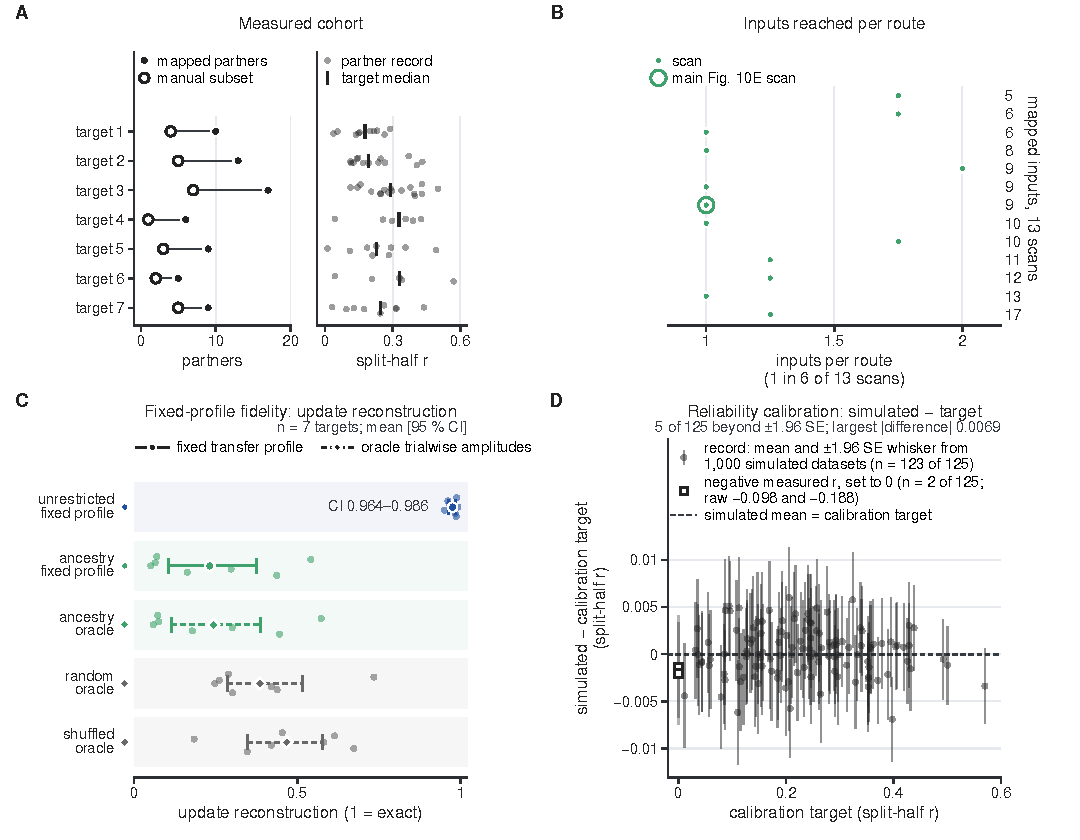
\includegraphics[width=\textwidth]{supplementary/curated/measured_transfer_geometry.pdf}
\caption{\textbf{The measured-response learning comparison is limited by mapped coverage and transfer geometry.} \textbf{A}, Number of mapped functional presynaptic partners for each of seven targets in one mouse. \textbf{B}, Actual four-route support for the scan selected by median mapped-input count, with identifier tie breaking; rows are input coordinates and columns selected routes. The selected supports are mostly single distal sites, rather than illustrative nested bands. \textbf{C}, Response-prediction NMSE for exact learning, treeless ridge and restricted dictionaries, with random and shuffled surrogate rows; dots are seven target means, diamonds and bars their means and 95\% target-bootstrap intervals, and the dotted line marks ridge. \textbf{D}, Common-checkpoint update reconstruction by the unrestricted fixed transfer profile, the restricted ancestry profile and oracle trialwise ancestry amplitudes. The unrestricted fixed profile is nearly sufficient because somatic error mainly scales a stable transfer vector; restricted rules underperform ridge. \textbf{E}, Mean split-half Spearman reliability in 1,000 independent calibration datasets versus the observed value, for 125 partner records; the two negative estimates are assigned zero reliable variance and the identity line is not fitted. Scans and splits are averaged within targets before inference; $n$ is seven targets in \textbf{C,D} and 125 partner--scan records in \textbf{E}, with 95\% bootstrap intervals throughout. Target-level associations for all four topology measures are in main Fig.~9C, and coverage across all thirteen scans is in main Fig.~9F. This is an offline passive-tree geometry diagnostic, distinct from the empirical ancestry-response association.}
\label{fig:si_measured_transfer_geometry}
\label{fig:supp_measured_detail}
\label{fig:supp_measured_alignment_power}
\label{fig:si_measured_topology}
\end{figure}

\begin{figure}[p]
\centering
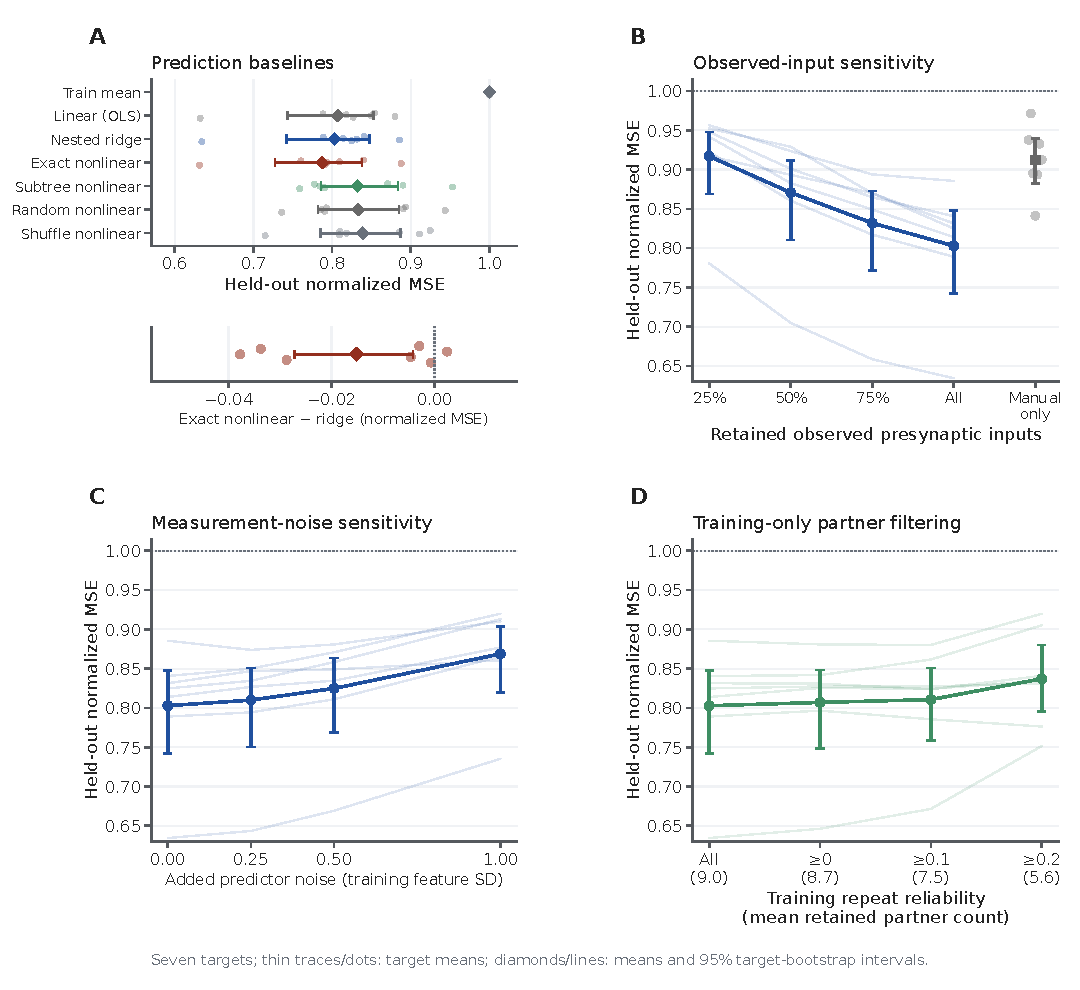
\includegraphics[width=\textwidth]{supplementary/curated/measured_predictor_controls.pdf}
\caption{\textbf{Linear baselines explain most measured-response prediction, and degrading observed inputs worsens performance.} Thirteen scans retain the complete-tree analysis's 130 outer stimulus-identity splits. All preprocessing, reliability masks and ridge tuning use training identities only. \textbf{A}, Training-mean, ordinary least-squares (OLS) and nested ridge-regression baselines against the matched nonlinear fits. Lower normalized MSE is better. Below, paired exact-nonlinear-minus-ridge differences show the small additional nonlinear benefit: mean $-0.0152$ (95\% interval $-0.0271$ to $-0.0042$). \textbf{B}, Ridge prediction when retaining nested random fractions of observed presynaptic inputs; five masks per split are averaged before inference. Manual-only partners are a separate provenance restriction, not a random retention dose. Empty masks use the training mean and remain included. \textbf{C}, Added Gaussian predictor noise in both training and test data, in units of training input standard deviation (SD) after the quantile transform. \textbf{D}, Reliability filtering based only on training repeats; parentheses give mean retained partner counts. Thin traces or dots show seven target means after averaging splits within scan and scans within target. Larger symbols and bars are means and 95\% target-bootstrap intervals (20,000 draws). All targets come from one mouse. Only ridge is refitted under the sensitivity conditions. Removing observed inputs does not recover unknown partners, establish population power or explain away the absence of preferential ancestry alignment.}
\label{fig:si_measured_predictor_controls}
\label{fig:supp_response_baselines}
\end{figure}

\begin{figure}[p]
\centering
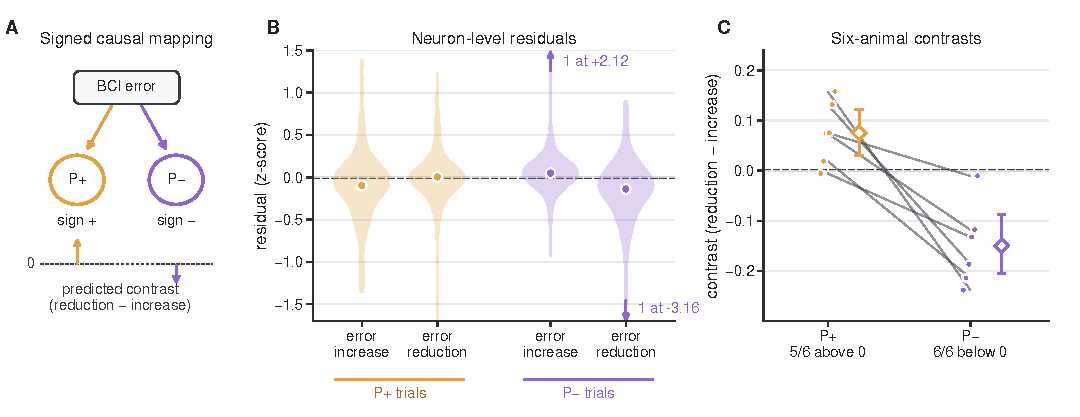
\includegraphics[width=\textwidth]{supplementary/curated/animal_credit_reanalysis.pdf}
\caption{\textbf{Published animal data are consistent with signed per-neuron teaching coordinates.} This reanalysis contains no reconstructed dendritic morphology and measures no within-tree learning signal; it tests only the sign of two neuron-level coordinates. \textbf{A}, In the source brain--computer-interface (BCI) experiment, P+ and P- populations had positive and negative causal decoder weights, predicting opposite dendritic residual contrasts. \textbf{B}, Descriptive neuron-level residual distributions from published source sheet ``5E'' for error-increasing (inc.) and error-reducing (red.) conditions, in the source z-score normalization; dots show means and bars show neuron-level standard errors. These bars are descriptive and are not animal-bootstrap intervals. The paired animal contrasts and mode-energy decomposition use $n=6$ animals and are reported in Table~\ref{tab:animal_credit}; animals are the inferential units for those tests. This retrospective external comparison is consistent with signed per-neuron information but does not resolve within-tree transport or uniquely identify a conductance mechanism. This reanalysis is restored as a figure so that the six-animal signed-credit comparison described in Methods has drawn support; the animal-level contrasts remain tabulated.}
\label{fig:si_animal_credit_reanalysis}
\label{fig:supp_animal_credit}
\end{figure}

\clearpage

% Curated from paper commit 7ee9157; original equations and protocol identities retained.
\section{Additional structure-selection analyses}
\label{note:selection_statistics}

\subsection{Prospective costed selection in tree-constrained linear learning}
\label{note:prospective_selection}

These secondary studies test structure selection separately from the main
credit comparisons. The first asks whether an initialization descent bound
can select a model for later learning. Five explicit 15-node trees supplied
eight labeled leaves: four balanced hierarchies with distinct leaf orders
and one contiguous comb. Each supplied orthonormal subtree-cut dictionaries
at $K=1,2,4,8$, giving 20 candidates per arm. Every candidate retained 64
trainable leaf-input weights. In the feedback-only arm, all candidates used
identity forward transfer $H_T=I_8$. In the joint arm, $H_T$ was the leaf
block of $(I_{15}+\kappa L_T)^{-1}$, where $L_T$ was the full-tree weighted
Laplacian, $\kappa=1$, unit leak was present at every node and edge
conductance was inverse embedded length. Internal nodes were retained.
For input $\bm x\in\mathbb R^8$, trainable weights
$W\in\mathbb R^{8\times8}$ and an imposed context decoder
$\bm a\in\mathbb R^8$, the scalar prediction was
$\bm a^{\mathsf T}H_TW\bm x$. Here $W$ denotes model weights. This passive-tree linear abstraction uses an imposed context readout, not a somatic voltage or the nonlinear physical-depth model.

A random orthogonal teacher mapped isotropic Gaussian inputs to labels.
Context decoders were sampled uniformly from the first $r$ columns of an
orthogonal basis $Q$, with $r\in\{1,2,4,8\}$ specifying the reference
credit rank. Observation-noise standard deviation (SD) was $\sigma_y=0$
or 0.75. At zero initialization, the exact reference
decoder-space credit second moment was
\[
S_0=(1+\sigma_y^2)Q\operatorname{diag}
(\underbrace{1/r,\ldots,1/r}_{r},0,\ldots,0)Q^{\mathsf T}.
\]
Rotation preserves this reference spectrum, but the joint arm's transfer can change transported-credit and parameter-gradient spectra. Angle and noise
comparisons shared underlying random draws within seed and rank. Five
development seeds (6100--6104) used angles $0,\pi/4,\pi/2$; 20 separate
confirmation seeds (7200--7219) used held-out angles $\pi/8,3\pi/8$.
The 16 rank--noise--angle conditions within each confirmation seed were
paired, giving 320 tasks per arm.

For dictionary projector $P$, the actual synaptic descent direction was
$\bm d_i=P H_T^{\mathsf T}\bm a_i\delta_i\bm x_i^{\mathsf T}$,
where $\delta_i$ was the scalar prediction error on example $i$. Inner products and covariances use the vectorized 64-coordinate update. Coefficients receive the known decoder and transfer, rather than a learned local encoder. Each candidate had
64 fixed task-decoder coefficients, $K$ channels, $8K$ possible context-to-
route encoder coefficients, eight nonzero delivery entries, 15 electrical
nodes and 14 edges. Let $\ell_T$ be the total cable length in the fixed two-dimensional
embedding and $\ell_{\max}$ the largest candidate length. The normalized
geometric cable cost was $\ell_T/\ell_{\max}$; the resource cost was
$C_T=K/8+0.1\ell_T/\ell_{\max}$. This declared cost proxy does not measure biological expenditure. Candidates with identical projectors but different cable costs remain identified as equivalence classes, not replicates.

Independent calibration, training and test sets contained 1,024, 2,048 and
4,096 examples. Calibration evaluated the actual routed update mean and
empirical single-example covariance, giving
$\E\|\bm d_{\mathrm{batch}}\|^2
=\|\E\bm d_i\|^2+\operatorname{tr}\operatorname{Cov}(\bm d_i)/32$
for minibatches of 32 independent and identically distributed (iid) draws. The initialization score was the bound at the
actual step $\eta=0.35$,
\[
U_T=\eta\bm g^{\mathsf T}\E\bm d_i-
\frac{\eta^2L_T^{\mathrm{cal}}}{2}
\left(\|\E\bm d_i\|^2+
\frac{\operatorname{tr}\operatorname{Cov}(\bm d_i)}{32}\right).
\]
Here $L_T^{\mathrm{cal}}$ is the largest Hessian eigenvalue of calibration half mean squared error (MSE), global in $W$. The bound concerns calibration loss, not independent-test or population loss. All weights
started at zero. Paired candidates received the same iid minibatch stream
for 256 updates, with checkpoints at 16, 64 and 256. Only the final checkpoint
defined the primary endpoint, test half-MSE plus $0.08C_T$.

Development's 4,800 fits fixed one nonnegative utility-to-final-loss scale $s\in[0,256]$ per arm, using within-task centered outcomes. The moment policy minimizes $\mathcal L_{\rm cal}(0)-sU_T+0.08C_T$. Development also fixes the constant, maximum-budget and known-rank policies; sampled and exact-expected random choice are references. All 3,200 confirmation choices were hash-sealed before training without retuning. The prospective protocol retains all 12,800 confirmation fits and 38,400 checkpoint rows, with no outcome exclusions.

Regret subtracts the retrospectively best candidate's costed loss on each task; this oracle is unavailable to selection. Intervals use 10,000 bootstrap draws over 20 whole-seed averages.
Moment-policy regret was 0.08055 (95\% interval 0.07262--0.08781) for
feedback-only selection and 0.10404 (0.09975--0.10791) for joint selection.
Fixed maximum-budget regret was 0.04495 and 0.04269; rank-only regret was
0.00831 and 0.00821. The moment selector lost to both in every seed average
in both arms. Rank-only improved over fixed by 0.03664 (0.03630--0.03697)
and 0.03448 (0.03427--0.03468). The retrospectively best budget equaled
the imposed rank on every confirmation task, while the contiguous balanced
tree won 308/320 feedback-only and 303/320 joint tasks. Thus the constructed family supports rank-dependent capacity but little fine tree selection.

Post hoc checks separate this failure from local prediction: the bound held in all 12,800 calibration conditions, and utility correlated 0.984/0.974 with first-update test improvement. Algebraic, covariance, derivative and source checks passed; 120 independent endpoints replayed within $5.55\times10^{-17}$. Complete matrices, policies and audits are in \texttt{source\_data/prospective\_morphology\_selection/}.

\subsection{Finite, noisy calibration of interaction-based tree selection}
\label{note:finite_calibration_morphology}

The finite-calibration study uses the eight-input, 28-coefficient model and twelve-candidate pool of Section~\ref{note:interaction_structure}, with four equally weighted families: four disjoint pairs, two complementary quartets, nested products of degrees 2/4/6/8, and a random-interaction control selecting four distinct degree-2--8 monomials. Input permutations, coefficient signs and magnitudes $\mathcal U[0.5,1.5]$ vary by task; coefficients are normalized to unit squared norm. Targets have zero mean and unit variance on uniform Rademacher inputs, without matched spectra across families.

The estimator receives input/output examples and all 255 nonconstant Walsh monomials, without family, planted support, true coefficients or derivatives. Lasso fits an unpenalized intercept and uses penalty $c\operatorname{sd}(y)\sqrt{2\log(256)/n_{\rm fit}}$, cyclic coordinate descent, tolerance $10^{-8}$ and at most 20,000 iterations. Five development blocks select $c$ from 0.15/0.35/0.65, fixing 0.15. Calibration budgets 64/256/1,024 cross Gaussian label-noise SD 0/0.5. The first 75\% of observations fit the estimator and pilots; the final 25\% is a calibration gate. Primary calibration therefore uses 192 fit observations out of 256 queries at SD 0.5.

The selector minimizes the maximum normalized centered-cut tail beyond rank one, breaking $10^{-10}$ ties by summed tails and candidate identifier. Only true-coefficient maximum tails are bounds; estimated tails and summed-tail tie-breaking are scores. Secondary subset dynamic programming searches beyond the pool at the primary condition.

Development fixes a constant candidate and an estimated-rank rule using the rank that explains 99.5\% of estimated input-gradient energy. Both reduce to \texttt{balanced\_p0}; sparse bins use the constant fallback. Other references are fixed shape representatives, exact uniform-random candidate expectation and a two-sweep ALS pilot. The pilot fits every candidate from one fixed initialization on the calibration-fit subset and chooses by gate MSE, then discards all pilot parameters. True-coefficient selectors and the retrospective best-trained candidate are privileged references.

Twenty new seed blocks supply eighty tasks; calibration inputs, scores, choices and adaptive trees were sealed before fitting. Pre-fit implementation repairs preserved those choices and are recorded in Source Data. Final fitting uses separate 1,024-example training data with noise SD 0.3, 32 ALS sweeps, two paired random restarts and output-preserving gauge normalization. Independent 512-example noisy validation chooses the restart. Twelve fixed candidates, one estimated adaptive tree and one true-coefficient adaptive reference give 2,240 fits; fixed candidate outcomes are reused across calibration conditions.

Primary evaluation uses clean-target MSE on 4,096 independent inputs and unit population variance; noisy-test and all-256-pattern errors are secondary. Streams can repeat patterns with independent observation identities/noise. Regret subtracts the best validation-selected fixed-pool result, retaining negative adaptive regret. Failed/nonfinite fits receive loss $10^6$, with warnings and counts retained.

The primary 256-query/noise-0.5 comparisons against development-best fixed and the two-sweep pilot use 10,000 whole-seed bootstrap draws, averaging families within seed, Bonferroni-adjusted 97.5\% intervals and a 0.01-NMSE margin. Other comparisons are descriptive. The exponential Walsh dictionary and ALS fitter constrain scalability and biological interpretation. Full outcomes and costs are in Source Data and Supplementary Fig.~\ref{fig:si_morphology_estimation}.

\subsection{Direct confirmation from noisy morphology estimates to gradient learning}
\label{note:morphology_end_to_end}

Twenty independent seed blocks 930910--930929 generate eighty new functions from the same four-family mixture. The fixed Lasso ($c=0.15$) receives 192 of 256 calibration observations at label-noise SD 0.5; the remaining 64 are reserved, unused. All estimated trees are hash-sealed before learning. The earlier best fixed balanced tree and a post-seal true-coefficient construction are references. Construction coefficients never initialize training.

Each of three trees receives exact path credit or unit root broadcast, giving 480 fits. The seven multi-affine units, 28 coefficients and root-only output are unchanged; broadcast replaces six nonroot sensitivities by one. All conditions share Gaussian nonbias initialization of SD 0.5, zero biases and independent calibration/training/test/minibatch streams. Coefficients remain in $[-2,2]$ and gradients are clipped at norm ten. Adam uses $(0.9,0.999)$ and $\epsilon=10^{-8}$, with inherited rates 0.01 for exact and 0.003 for broadcast. Thus comparisons are between frozen recipes, not common rates.

Learning uses 1,024 updates of 64 examples from a 2,048-example cache with label-noise SD 0.15, minimizing half-MSE divided by known target variance. Separate 4,096-example test data use fresh noise. No validation selection, retuning or continuation from calibration fits occurs. Primary noisy-test NMSE has expected floor 0.0225; clean test and all-pattern errors are secondary. Within-seed family-averaged comparisons use 10,000 bootstrap draws, adjusted 97.5\% intervals for the two primary contrasts and the same 0.01 effect margin. Fixed-minus-estimated exact-credit error was 0.45913 $[0.38489,0.53227]$; broadcast-minus-exact on estimated trees was 0.60750 $[0.56916,0.64610]$. Matching, quartet and nested tasks approached the floor with estimated-tree exact credit, while random interactions retained error and broadcast performed slightly better on matching.

Six full-horizon checks (seed 721000) are excluded; a documented pre-fit repair preserved settings and choices. Independent reconstruction reproduced all eighty trees and endpoints exactly. All 480 trajectories and validation records are in \path{source_data/morphology_calibration/end_to_end}. The pipeline demonstrates finite-data construction and learning within this class, not endpoint-optimal morphology.

\subsection{Finite-horizon forecasts for the contextual linear learner}
\label{note:finite_horizon_morphology}

A finite-horizon predictor tests the failed scalar extrapolation while retaining the candidate pool, $\eta=0.35$, minibatch size $B=32$, 256-update horizon and cost. Five original development seeds informed its design; the predictor was frozen before fresh calibration or training. Twenty new seeds (9300--9319)
crossed four ranks, two noise levels, two held-out angles, both transfer arms
and both training regimes. Every candidate was trained, yielding 25,600 new
fits and 76,800 checkpoint outcomes at updates 16, 64 and 256. Non-pilot scores were sealed before each seed's outcomes without endpoint tuning. The predictor separates mode-dependent dynamics from a scalar initial slope, motivated by deep linear learning and task alignment with kernel eigenfunctions \citep{lampinen2019generalization,canatar2021spectral}.

To forecast learning, we express the weights in route coordinates. For
orthonormal routes $\Phi$, the learner stays in $W=\Phi V$. For context
$j$ with decoder $\bm a_j$, define the effective route vector
$\bm c_j=\Phi^{\mathsf T}H_T^{\mathsf T}\bm a_j$.
The scalar prediction is $\bm c_j^{\mathsf T}V\bm x$ and the actual update
is minibatch descent in $V$. Let $\bm v=\operatorname{vec}(V)$ stack the route-coordinate weights.
For calibration example $i$ with input $\bm x_i$, label $y_i$ and effective
route vector $\bm c_i$, define
$\bm z_i=\operatorname{vec}(\bm c_i\bm x_i^{\mathsf T})$. With
$\E_i$ denoting an average over the calibration-fit examples, set
$H_{\rm emp}=\E_i[\bm z_i\bm z_i^{\mathsf T}]$ and
$\bm b_{\rm emp}=\E_i[y_i\bm z_i]$. Write
$H_{\rm emp}=U\operatorname{diag}(\lambda)U^{\mathsf T}$, with orthonormal
eigenvectors in $U$ and eigenvalues in $\lambda$. After $T$ updates,
full-batch descent from zero gives
\begin{equation}
 \bm v_T=U\operatorname{diag}\!\left(
 \frac{1-(1-\eta\lambda)^T}{\lambda}\right)U^{\mathsf T}\bm b_{\rm emp},
 \label{eq:s_spectral_forecast}
\end{equation}
The diagonal expression is evaluated separately at each eigenvalue, with
continuous value $\eta T$ when that eigenvalue is zero. The empirical selector
fits the first 512 calibration examples and evaluates on the other 512;
Eq.~\ref{eq:s_spectral_forecast} is exact for that full-batch surrogate,
not for the original cached-data SGD process.

For fresh inputs $\bm x\sim\mathcal N(0,I_d)$, where $d$ is the input
dimension, a smaller recurrence describes stochastic gradient descent (SGD).
Let $p_j$ be the context probabilities and $\bm t_j\in\mathbb R^d$ the
target coefficient vector in context $j$. Suppose
$y=\bm t_j^{\mathsf T}\bm x+\epsilon$, with independent zero-mean noise
of variance $\sigma_j^2$. The exact recurrence closes on the mean weights
$M=\E[V]\in\mathbb R^{K\times d}$ and the route-space variance matrix
$\Gamma=\E[(V-M)(V-M)^{\mathsf T}]$. The latter sums weight covariance
over the input coordinates; it is not the full vectorized parameter
covariance. Define
\begin{align}
 C&=\sum_jp_j\bm c_j\bm c_j^{\mathsf T},&
 D&=\sum_jp_j\bm c_j\bm t_j^{\mathsf T},&
 \bar G&=CM-D,\\
 R_j&=\|M^{\mathsf T}\bm c_j-\bm t_j\|^2+
                    \bm c_j^{\mathsf T}\Gamma\bm c_j,&
 A_\eta&=I-\eta C,\\
 J&=\sum_jp_j\bm c_j\bm c_j^{\mathsf T}
                  [(d+2)R_j+d\sigma_j^2],&
 K_G&=C\Gamma C+\bar G\bar G^{\mathsf T}.
\end{align}
Here $\bar G$ is the mean gradient, $R_j$ is the expected squared residual
excluding observation noise, $J$ is the second moment of the single-example
gradient Gram matrix, and $K_G$ is the corresponding second moment of the
conditional-mean gradient. For a fixed residual coefficient vector
$\bm e$, Gaussian fourth moments yield
$\E[(\bm e^{\mathsf T}\bm x-\epsilon)^2\|\bm x\|^2]
=(d+2)\|\bm e\|^2+d\sigma_j^2$. Conditioning first on the current
weights, the Gram of a minibatch-mean gradient is its conditional-mean Gram
plus $1/B$ times its conditional variance. Total covariance therefore gives
\begin{align}
 M_{t+1}&=M_t-\eta\bar G_t,\\
 \Gamma_{t+1}&=A_\eta\Gamma_t A_\eta^{\mathsf T}
                      +\frac{\eta^2}{B}(J_t-K_{G,t}),
 \label{eq:s_fresh_sgd_moments}\\
 \E[\mathcal L_T]&=\tfrac12\sum_jp_j[R_j(T)+\sigma_j^2].
\end{align}
The forecast updates noise with the residual and weight variance. It requires Gaussian input fourth moments and fresh independent minibatches; noise needs only the stated first two moments. This closure does not cover nonlinear targets, anisotropic inputs, adaptive optimizers or correlated samples.

The primary plug-in predictor estimates context frequencies, conditional
coefficient vectors and residual noise variances using 1,024 independent
calibration examples. Coefficients use ordinary least squares without an
intercept, and noise variances use residual degrees of freedom. Its recurrence
is exact for the fitted Gaussian population and is a plug-in approximation
for the generating population. Population-oracle versions instead receive
true teacher coefficients and noise moments and are labeled privileged.
The 16-step pilot performs real candidate updates and evaluates on
calibration observations; its computation is included. An observed-context-
count baseline chooses the smallest permitted $K$ covering the number of
distinct observed context vectors, followed by the cheapest tree. This and an observed-count-restricted conditioning baseline were frozen after development inspection, before new outcomes. Context count equals generating rank only in this constructed family.

We ran both fresh-example SGD and minibatches resampled from a fixed
2,048-example cache, retaining a common 4,096-example test set. Reusing a
cache makes later weights dependent on those examples and violates the fresh
recurrence's independence assumption. Population-oracle prediction minus
exact population loss of the realized weights quantifies that discrepancy.
All conditions are averaged within seed before 10,000 whole-seed bootstrap draws. Pointwise intervals for secondary comparisons carry no multiplicity-adjusted confirmation claim. Numerically constant cases retain undefined correlations with explicit defined-task counts, without outcome exclusions.

Supplementary Fig.~\ref{fig:si_finite_horizon} shows endpoint
regret and strong baselines, selection timing, and the forecast-versus-outcome
comparisons; the joint-arm cache sensitivity is retained in Source Data.
The complete timing and prediction outcomes are in Source Data (Table~\ref{tab:source_index}). The primary forecast reaches mean fixed-cache
regret $0.000064$ and $0.000042$ in the feedback and joint arms, while the
cheap observed-count baseline reaches $0.000134$ and $0.000197$. The scalar-score improvement therefore does not establish a large fine-selection advantage. Tests verify spectral forecasts against direct descent, stochastic moments against Gaussian quadrature, sealed choices and exclusion of training/test observations from predictors. Complete data, protocols and source hashes are in
\path{source_data/morphology_structure/} and
\path{source_data/morphology_finite_horizon/}.
\subsection{Statistical analysis, reproducibility and interpretation}
\label{note:statistics}

Central comparisons report paired effect sizes, the number of positive cell
or seed pairs, and 95\% intervals unless a different level is specified for
that analysis. Tests were two sided unless a direction had been specified
before analysis. Exact Wilcoxon signed-rank tests were used for
small paired cell cohorts. Reconstructed-cell intervals resampled cells first
and, where relevant, one Monte Carlo stream within cell. Measured-response
intervals resampled target cells. Artificial-network summaries used
independently initialized training runs. Inhibitory-census outcomes were first
averaged within postsynaptic target. Signed-credit intervals and exact sign
tests used animals; neuron-level source rows were descriptive only.

Bootstrap intervals used 20,000 draws unless an experiment's protocol states
otherwise; the Fashion-MNIST ladder, the physical-depth, H4 and task-family
cohorts and the external animal reanalysis used 50,000 paired draws.

Benjamini--Hochberg correction was applied within each prespecified comparison
family---the archived four-budget subtree scan across $K=1,2,4,8$, the six
bandwidth-matched routing contrasts and the H4 primary family. The additional four-budget ancestry-minus-best-control reanalysis enumerated
all $2^{20}$ paired sign assignments for a two-sided mean-difference test
and applied Holm correction across the four budgets. Accuracy differences
were reconstructed on the exact $1/2048$ test-count grid before testing.
Initialization-score correlation intervals used 5,000 whole-seed bootstrap
draws. The local-context soft-encoder analysis used Holm correction across its
three primary contrasts; the hard-readout follow-up remains exploratory. The prospective selection experiment resampled 20 whole seed blocks 10,000
times. The finite-horizon, morphology-calibration, credit and conductance studies
also used 10,000 whole-seed draws, retaining task, candidate and optimizer
conditions together within each seed. The two primary comparisons in each of the finite-calibration and
separate end-to-end experiments used Bonferroni-adjusted 97.5\% intervals and
a prespecified 0.01 improvement margin in normalized MSE (NMSE). Other bridge
intervals are pointwise and descriptive. Exhaustively enumerated structural targets have
no biological sampling interpretation. Response-baseline sensitivity retained seven
targets and 20,000 draws. Other parameter
sweeps and sensitivity analyses received no multiplicity correction, are
labeled secondary, and are not interpreted as independent confirmation.

Cross-mouse contrasts are summarized within volume; cell-level tests do not provide an animal-level $P$ value from two mice. The 12-cell Pinky
cohort was sized to span 12 equal-count spatial strata while keeping complete
mesh skeletonization and 500-shuffle processing feasible. The task-family
factorial used ten paired seeds, matching the sample size used for the
physical-depth experiments; positive directional language
requires a paired 95\% interval excluding zero and at least 8/10 seed signs.

Cross-architecture conclusions exclude pooled error-field metrics that mix
dendritic stages with a somatic stage whose reconstruction is exact by
construction. They also exclude unweighted path-gain dispersion as evidence
of gradient direction and post hoc comparisons between unmatched training
cohorts. Table~\ref{tab:claim_boundaries} records the supported
interpretation and boundary of each evidence class.

Each empirical main panel has a machine-readable table with values, independent and nested units, seeds, conditions and analysis version. Automated checks verify these figure inputs.
Authentication tokens, restricted caches, and raw data already hosted by
MICrONS or DANDI are not redistributed.

Source Data retain configurations, outcomes, exclusions, selections and hashes; software contains implementations, joins and figure builders. Manifests authenticate source identities and path translations without changing numerical settings. The source index maps compact tables to complete records.

An exact package lock was not archived for the June exact-transport or
backpropagation jobs, nor for the measured-response analysis. These versions
are therefore not guessed from the current environment. The complete July feedback analysis records Python 3.10.13, its Git identity
and selected source hashes. Its archived source state nevertheless includes
tracked modifications. Table~\ref{tab:regular_archive}
and the accompanying reproducibility README distinguish exact, partial and
unverifiable provenance fields.

\begin{figure}[p]
\centering
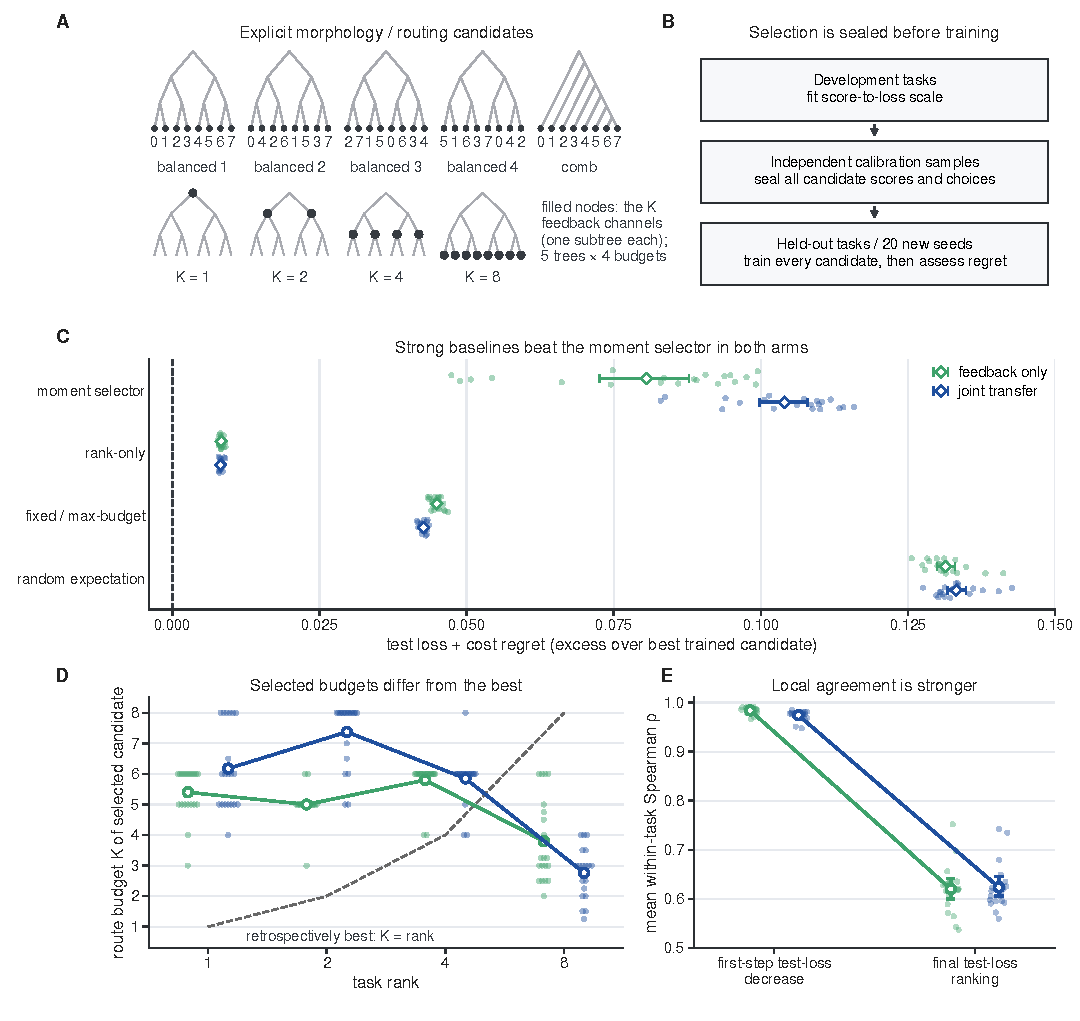
\includegraphics[width=\textwidth]{supplementary/curated/original_selector.pdf}
\caption{\textbf{The original scalar initialization score predicts a first step but fails at prospective endpoint selection.} \textbf{A}, Four balanced leaf assignments (balanced 1--4; the number under each leaf is the input index at that leaf slot) and one comb, each at route budgets $K=1,2,4,8$: twenty candidates with prescribed cost. Filled nodes mark the $K$ feedback channels, one subtree each. \textbf{B}, Development, independent calibration, sealed choices and confirmation training. \textbf{C}, Final test half-mean-squared-error (MSE) plus cost, expressed as excess over the best trained candidate, for the feedback-only (green) and joint passive-transfer (blue) arms; the dashed line marks zero regret. Small points are the twenty whole-seed means; open diamonds and whiskers are means and 95\% seed-bootstrap intervals (10,000 draws), which are narrower than the diamond in the rank-only, fixed / max-budget and random-expectation rows. The fixed / max-budget baseline (the development choice, which is also the maximum budget) and the privileged rank-only baseline outperform the moment selector; random expectation averages all candidates uniformly. \textbf{D}, Route budget of the candidate chosen by the moment selector versus imposed rank; small points are the twenty seed-block means, open circles their mean, and the gray dashed line the retrospectively best candidate's budget, which equals the rank in every task of both arms. \textbf{E}, Mean within-task Spearman correlation of initialization utility with the actual first-step test-loss decrease and with the final test-loss ranking; small points are the twenty seed-block means, open circles and whiskers their mean and 95\% interval resampling whole seeds ($n=20$ seed blocks). Colours in \textbf{D,E} as in \textbf{C}. All 12,800 confirmation candidate fits and 38,400 checkpoints remain included. Every model has a freely trained dense weight matrix; passive transfer changes conditioning and cost but does not necessarily restrict representation. This experiment is distinct from the locally connected multi-affine construction and the separately frozen finite-horizon follow-up.}
\label{fig:si_original_selector}
\label{fig:supp_original_prospective_selection}
\end{figure}

\begin{figure}[p]
\centering
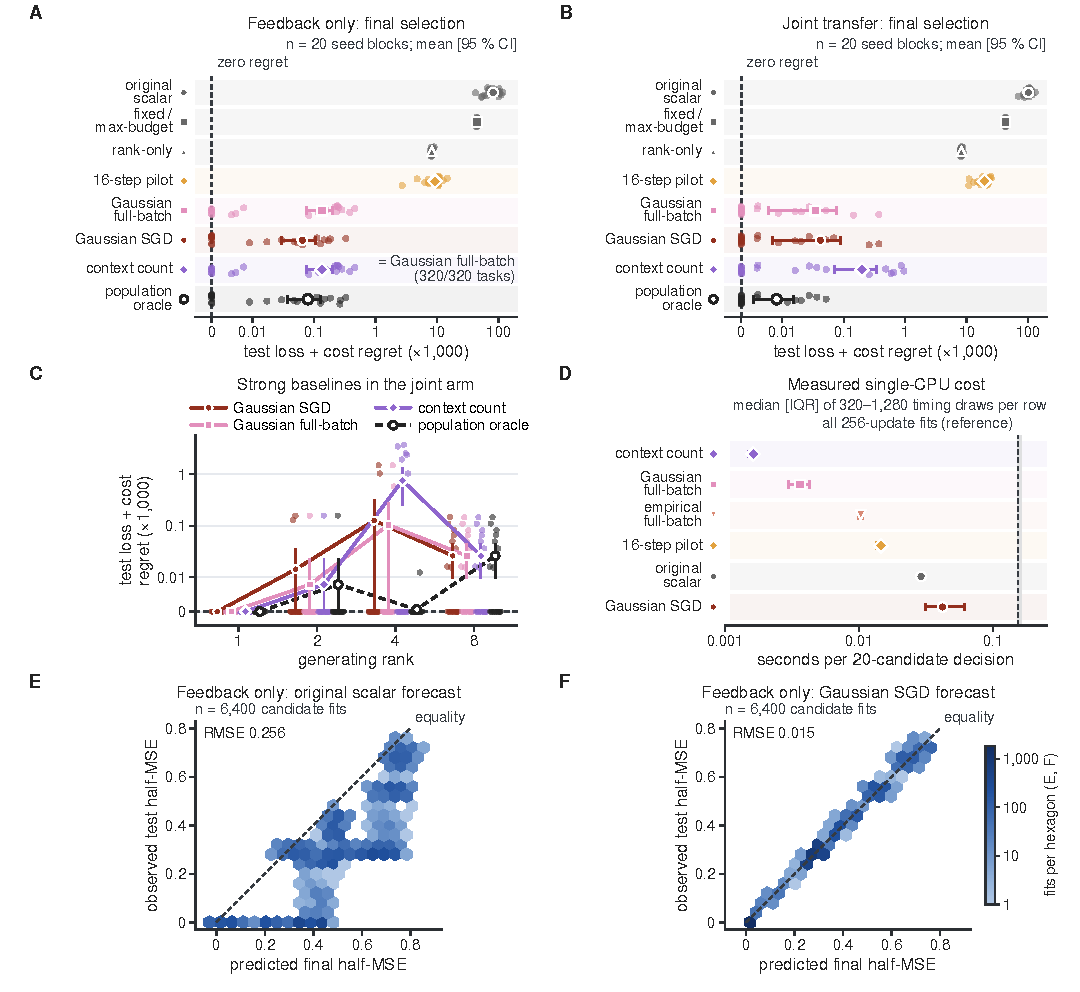
\includegraphics[width=\textwidth]{supplementary/curated/finite_horizon.pdf}
\caption{\textbf{Finite-horizon prediction improves selection but strong simple baselines remain.} \textbf{A,B}, Final costed-test-loss regret by imposed rank in the feedback-only and joint-transfer fixed-cache learners; regret is excess above the best trained candidate. \textbf{C}, Differences among strong selectors at each rank in the joint arm. The independently calibrated Gaussian SGD forecast improves over the original scalar utility; the full-batch and observed-context-count baselines remain competitive. All finite-horizon policies choose $K=r$ in this family, so improvement does not establish fine morphology selection. \textbf{D}, Median measured elapsed time on one central processing unit per twenty-candidate decision. Plug-in timings include calibration-model preparation, count-only time excludes shared calibration generation, and the pilot includes sixteen candidate updates; times measure these implementations, not hardware-independent complexity. \textbf{E}, Original scalar forecast versus final test half-mean-squared-error in the feedback-only arm. \textbf{F}, The calibration-derived Gaussian SGD forecast on the same cases and arm. Hexagons encode counts on a logarithmic color scale and dashed lines mark equality; the joint arm reproduces \textbf{E,F} and is retained in Source Data. The population-oracle forecast bias --- predicted minus exact population loss of the realized trained weights under fresh examples or finite-cache reuse --- is retained in Source Data: the fresh-example recurrence is exact under the stated Gaussian and conditional-linear assumptions, whereas cache reuse violates independence. Curves and whiskers in \textbf{A--D} are means and pointwise 95\% intervals from 10,000 whole-seed bootstrap draws over twenty seed blocks. All 25,600 candidate fits and both regimes are retained. These are linear-learning forecast tests, not a general nonlinear dendritic morphology law.}
\label{fig:si_finite_horizon}
\label{fig:supp_finite_horizon_selection}
\label{fig:supp_finite_horizon_prediction}
\end{figure}

\begin{figure}[p]
\centering
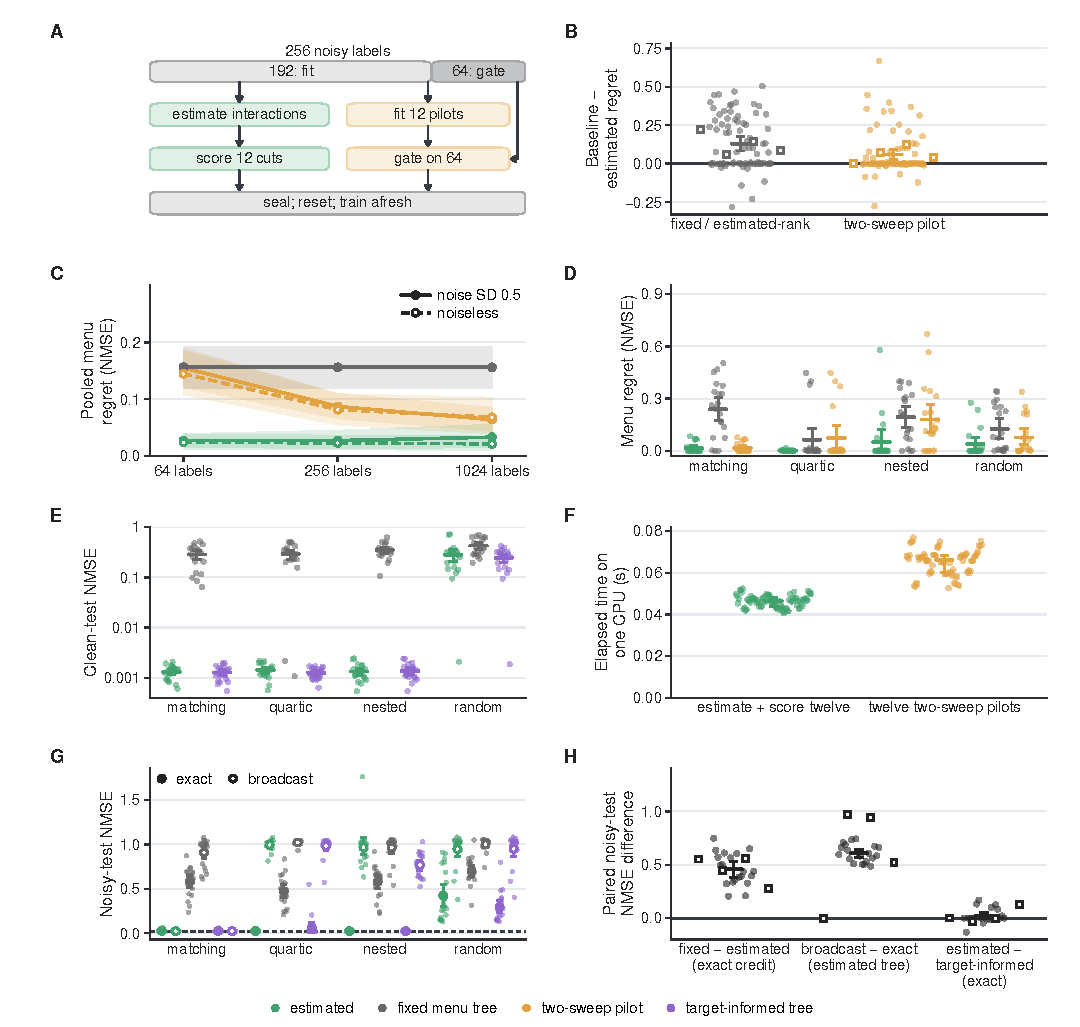
\includegraphics[width=\textwidth]{supplementary/curated/morphology_estimation.pdf}
\caption{\textbf{Finite calibration, adaptive construction and direct gradient learning.} \textbf{A}, Primary calibration: 256 labels, noise standard deviation (SD) 0.5; 192 observations for estimation/pilot fitting and 64 for pilot gating. The 255-term Walsh estimator receives no family labels, true support or coefficients. The pilot fits all twelve candidates for two sweeps. Choices are sealed; training restarts independently. \textbf{B}, Prespecified pooled fixed-baseline-minus-estimated and pilot-minus-estimated normalized mean squared error (NMSE). Whiskers are Bonferroni-adjusted 97.5\% paired bootstrap intervals; the dotted line marks the 0.01-NMSE meaningful-improvement margin. \textbf{C}, Excess clean-test NMSE above the best trained candidate across calibration sizes; solid curves use noise SD 0.5 and dashed curves no noise. \textbf{D}, Family-specific primary regret for estimated interactions, the development-fixed/estimated-rank baseline and the fitting pilot; pooled superiority is not uniform across families. \textbf{E}, Secondary adaptive trees trained with alternating least squares (ALS), versus the best trained twelve-candidate menu and a full-target construction oracle. Random-interaction errors remain. \textbf{F}, Elapsed time (median and interquartile range) on one CPU for eighty tasks: estimation/scoring of twelve trees versus pilot fitting/gating, excluding final training. \textbf{G,H}, Independent twenty-seed Adam cohort. \textbf{G}, Three structures and two credit rules in four non-isospectral families: filled symbols, exact credit (Adam 0.01); open, root broadcast (0.003). Label-noise floor: 0.0225; \textbf{E} uses clean targets. \textbf{H}, Fixed-minus-estimated error under exact credit and broadcast-minus-exact error on estimated trees use Bonferroni-adjusted 97.5\% intervals; estimated-minus-target-informed error under exact credit uses a pointwise 95\% interval. Target-informed construction is not a performance ceiling. Other whiskers: pointwise 95\% intervals, 10,000 whole-seed bootstrap draws ($n=20$); pooled statistics average families within seed. Both cohorts are independent of Supplementary Fig.~\ref{fig:si_oracle_profile_credit}.}
\label{fig:si_morphology_estimation}
\label{fig:supp_morphology_calibration}
\end{figure}

\clearpage

\section{Learned computations at retained checkpoints}
\label{note:checkpoint_computation}

This post hoc analysis makes the computations learned in main Figs.~5 and 6 visible. It uses every seed in each primary cohort and the original validation-selected states, without additional training, rate selection or selection of illustrative seeds. The two cohorts remain separate; they are not forty replicates of one experiment.

\paragraph{Single-neuron branch tuning.}
For each of the twenty opposed-target teacher--student seeds, we evaluated exact credit, the hard distal gate and broadcast at the primary Adam rate 0.03 and the state selected within 4,096 updates. Each seed's own teacher provides the reference. We varied the first feature over 65 values in $[-2,2]$ and integrated over the independent second feature using 32-point Gauss--Legendre quadrature for the uniform distribution on that interval. Context selected the left or right branch. The plotted quantity is the selected proximal branch's contribution to somatic voltage, $g_{p\to0}^{\rm den}V_p/(1+\sum_p g_{p\to0}^{\rm den})$, rather than its unweighted voltage: coupling changes can otherwise rescale an internal response without changing its somatic effect. Means and pointwise 95\% whole-seed bootstrap intervals use all twenty seeds and 10,000 resamples. The exact and gated learners recover the opposing tuning curves closely; broadcast produces weaker feature modulation (Fig.~\ref{fig:si_checkpoint_computation}A,B).

\paragraph{Population response surfaces.}
We evaluated all twenty original-bound Adam rescue seeds for resistance gating, augmentation and exact credit at their original selected rates and checkpoints. The model code is the verified execution snapshot. Each selected stream was evaluated on a uniform $25\times25$ feature grid over $[-2,2]^2$. At each grid point, sixteen fixed antithetic draws of the irrelevant streams approximate their uniform marginal distribution; the same draws are shared across rules and seeds. We multiply predictions by $(-1)^c$ to align the target sign across the four contexts, then average contexts within each seed. This makes the common target $T(z_1,z_2)=(\tanh z_1+\tanh z_2)/2+\tanh z_1\tanh z_2/4$. The plotted surfaces are seed means, not individual favorable examples. Per-context predictions are retained in Source Data.

To isolate the interaction, we subtract both one-feature marginal means and add the grand mean. With normalized trapezoidal grid weights $w$, this is
\[
I[F]_{ij}=F_{ij}-\sum_k w_kF_{ik}-\sum_k w_kF_{kj}+\sum_{k\ell}w_kw_\ell F_{k\ell}.
\]
The target interaction is $I[T]=\tanh z_1\tanh z_2/4$. Resistance gating reproduces much of the additive component but severely underestimates this interaction; augmentation and exact credit reproduce both (Fig.~\ref{fig:si_checkpoint_computation}C--J). For each seed we also report grid-weighted squared component error divided by target-component squared amplitude. Mean relative interaction error is 0.783 for resistance, $6.1\times10^{-5}$ for augmentation and $6.7\times10^{-5}$ for exact credit; corresponding additive errors are 0.00100, $1.0\times10^{-5}$ and $7.6\times10^{-6}$. These descriptive, context-averaged grid errors are not the ordinary-test NMSE and do not replace its primary comparisons. Marginalization and averaging can hide context-specific or seed-specific errors; the per-seed component values and per-context surfaces are retained. This analysis characterizes the existing selected states and does not establish a new convergence result.

Source records under \path{source_data/checkpoint_computation/} include the evaluation protocol, verified input hashes, all curves and surfaces, component errors and plotted summaries. The analysis script is \path{scripts/review_completion/checkpoint_computation.py}; the figure is rebuilt by \path{scripts/review_completion/checkpoint_figure.py}.

\clearpage
\begin{figure}[p]
\centering
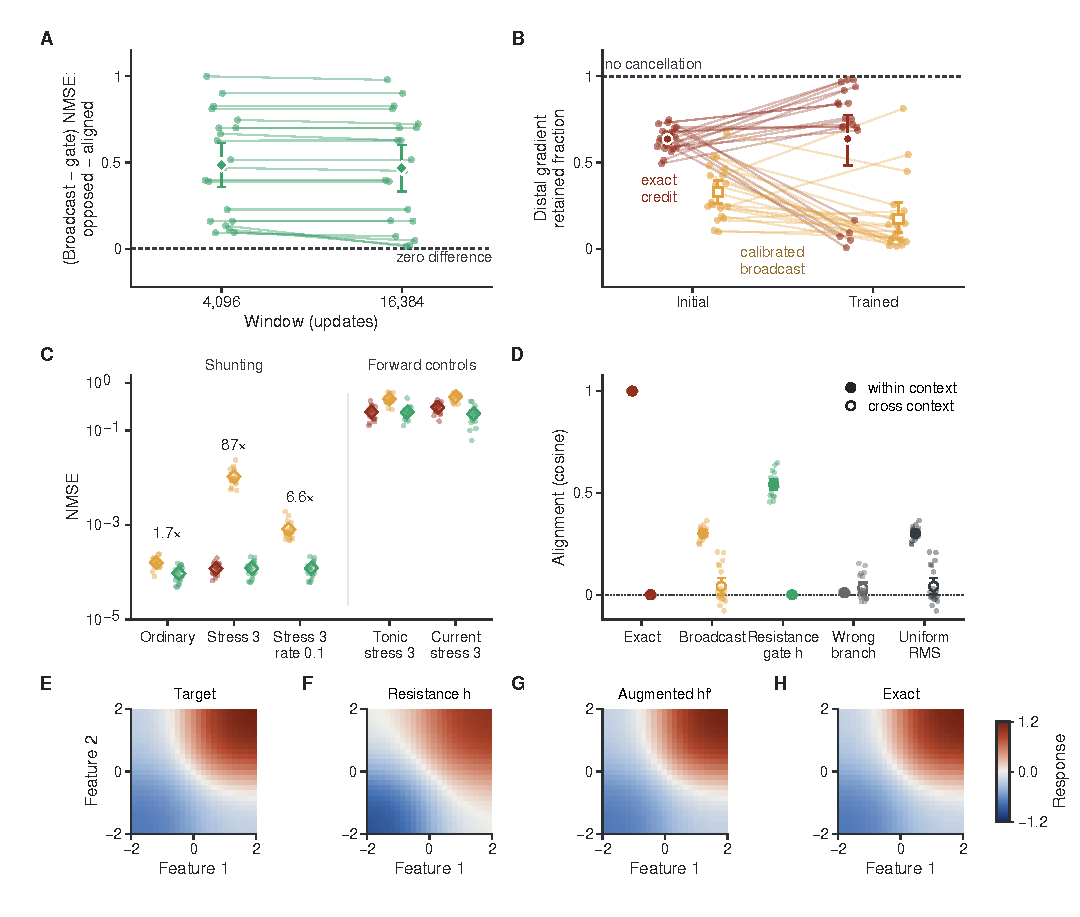
\includegraphics[width=\textwidth]{supplementary/curated/checkpoint_computation.pdf}
\caption{\textbf{Checkpoint responses show preserved branch tuning and recovery of the target interaction.}
\textbf{A,B}, Selected left/right proximal branches' contributions to somatic voltage in the opposed-target single-neuron task. Feature 1 varies; feature 2 is integrated over its uniform distribution. Dashed grey, teacher; amber, broadcast; green, hard distal gate; dotted red-brown, exact credit. Exact and gated curves nearly coincide. Lines and bands are means and pointwise 95\% whole-seed bootstrap intervals over twenty seeds, using the primary rate and validation-selected states within 4,096 updates.
\textbf{C--F}, Nonlinear-population target and learned response surfaces, with a common color scale. Predictions are averaged over sixteen irrelevant-stream draws and four sign-aligned contexts within each seed, then over the twenty rescue seeds. Each rule retains its original selected Adam rate and checkpoint. Feature axes span the ordinary training range.
\textbf{G--J}, The same surfaces after subtracting both one-feature marginal means and adding the grand mean. The shared interaction scale is distinct from the response scale above. Resistance gating underestimates the interaction; augmented and exact credit recover it. Colors encode response values, not learning-rule identity.
These are post hoc descriptions of existing checkpoints, with no new training cohort or outcome-based choice of examples. Full per-seed and per-context values are in Source Data: \texttt{checkpoint\_computation/}.}
\label{fig:si_checkpoint_computation}
\end{figure}
\clearpage


% Compact tables; repeated endpoint grids are available in the indexed Source Data.
\phantomsection
\section*{Reference tables and source-data index}
\addcontentsline{toc}{section}{Reference tables and source-data index}

\begin{table}[tbp]
\centering
\caption{Delivery profiles and coefficient sources. A useful span and an implementable coefficient rule are separate requirements.}
\label{tab:feedback_objects}
\small
\begin{tabularx}{\textwidth}{p{0.23\textwidth}X}
\toprule
Comparison & Field, information source and model \\
\midrule
Images & Twelve nonsomatic activation coordinates per $[3,3]$ tree. Neuron-specific error is supplied by the exact linear readout; $K=1/K=3$ coefficients project the exact activation field. Local output derivatives remain in eligibility. \\
Quadratic screens & Sixteen abstract parameter coordinates; exact/noisy projections and supplied or paired-probe reliability estimates. No forward neuron is simulated in the Haar screens. \\
Context and ancestry & Eight terminal blocks receive $\delta_i\Phi_{c_i,:}$. Context is supplied; the separate cue encoder learns coefficients before task training. \\
Multi-affine trees & Six nonroot unit errors receive exact paths, a unit or initial signed profile, or oracle-projected coefficients. Best-rank-one capture is a separate common-state diagnostic. \\
Conductance learning & Six nonsomatic voltages. Three-profile coefficients use current exact paths. Two leaf profiles plus unit proximal credit retain oracle amplitudes. The hard local rule instead gates distal somatic error by parent inhibition, retaining unit proximal credit; all 24 conductances learn. \\
Reconstructed arbors & Weighted input sites; broadcast plus ancestry supports. Free projection coefficients measure capacity for modeled passive fields. No encoder or biological learning is measured. \\
Measured-response models & Four-route spans contain one frozen baseline-transfer profile scaled by output error. Trialwise field/update oracles are geometry diagnostics and are not trained. \\
\bottomrule
\end{tabularx}
\end{table}

\begin{table}[tbp]
\centering
\caption{Regular-tree execution records. Missing historical software versions are not inferred from a current environment. Complete configurations, manifests and exclusion ledgers accompany Source Data.}
\label{tab:regular_archive}
\small
\begin{tabularx}{\textwidth}{p{0.26\textwidth}X}
\toprule
Cohort & Retained provenance \\
\midrule
120 MNIST feedback runs & Configurations, checkpoints, logs and hashes; Python 3.10.13; source identities \texttt{6c1aaa25}/\texttt{bd5f905e}. Scientific signatures and executable sources match across fields within architecture. Heterogeneous NVIDIA devices. \\
60 gradient-diagnostic runs & Same records; Python 3.10.13, source \texttt{4ba38bde} with archived tracked modifications and explicit source hashes; H200, 4.006 summed GPU-hours. \\
640 depth-feedback runs & 480 conductance-valid retained; configurations, curves, resource records and the complete validity ledger. Later inactive-source edits were checked for numerical equivalence. Heterogeneous NVIDIA devices, 73.29 summed GPU-hours. \\
160 diagnostic checkpoints & 120 valid; five fields/four step sizes per checkpoint, paired/clustered analysis and complete exclusions. No new training. \\
320 exact/BP repeats & Unmodified root \texttt{74792ca}, nested generator \texttt{4f3612a5}, configurations, seeds, checkpoints and scheduler records; H200. Signed additive and ReLU shunting inputs remain distinct. \\
20 exact-factorial / five BP references & Configurations, checkpoints, logs and grouped outcomes on A100-SXM4-40GB; 2.953/0.474 summed GPU-hours. Exact commit, Python and package versions were not recorded. \\
\bottomrule
\end{tabularx}
\end{table}

\begin{table}[tbp]
\centering
\caption{Repeated exact-transport/BP outcomes, averaged over four depths within each of ten paired seeds. Accuracy is a percentage and the contrast is percentage points, with a 20,000-draw paired 95\% interval. The full seed contrasts and descriptive tests remain in Source Data.}
\label{tab:clean_exact_bp}
\small
\begin{tabularx}{\textwidth}{p{0.28\textwidth}rrX}
\toprule
Task and core & Exact & BP & Exact minus BP (95\% interval) \\
\midrule
MNIST, raw additive & 97.013 & 97.008 & $0.005$ ($-0.028$ to $0.041$) \\
MNIST, shunting & 96.960 & 96.973 & $-0.013$ ($-0.047$ to $0.022$) \\
Noisy lines, raw additive & 33.378 & 33.490 & $-0.112$ ($-0.465$ to $0.247$) \\
Noisy lines, shunting (ReLU) & 36.690 & 36.788 & $-0.098$ ($-0.653$ to $0.390$) \\
\bottomrule
\end{tabularx}

The 320 runs form 160 method pairs. One depth-averaged MNIST additive seed was tied. Exact transport is an information-oracle implementation control; an interval containing zero is not an equivalence test.
\end{table}

\begin{table}[ht]
\centering
\caption{Outcome-independent conductance-validity accounting for the artificial-tree experiments. ``Included'' counts retained training runs, or checkpoints in the diagnostic row; these unit types are not added together. The entire inhibitory-dose family is excluded because its prespecified endpoint compares against invalid signed-input shunting cells.}
\label{tab:input_validity}
\small
\begin{tabular}{lrrrr}
\toprule
Experiment & Planned units & Invalid shunting & Unmatched controls & Included units \\
\midrule
Depth by feedback & 640 runs & 160 & 0 & 480 \\
Matched routing & 160 runs & 40 & 0 & 120 \\
Inhibitory dose & 400 runs & 200 & 200 & 0 \\
Spatial topology & 320 runs & 80 & 0 & 240 \\
Fixed-budget depth & 320 runs & 160 & 0 & 160 \\
Checkpoint diagnostic & 160 checkpoints & 40 & 0 & 120 \\
\bottomrule
\end{tabular}

\vspace{4pt}
\small The exclusion rule is task plus core plus resolved transfer
activation; no accuracy or gradient outcome enters it. The complete 1,840-run
validity table and all included row tables are supplied as Source Data.
\end{table}

\begin{table}[ht]
\centering
\caption{Complete reconstructed-tree learning across all eligible scans. Means average ten held-out-stimulus splits within each of 13 scans, then scans within each of seven target cells. Mean squared error (MSE) is normalized to the training-mean predictor. Each restricted learning rule scales one fixed site profile in a four-route span by scalar prediction error. Common-checkpoint update match is one minus normalized squared update error for that prescribed profile, rather than the best attainable projection into the full span.}
\label{tab:functional_full_tree}
\small
\begin{tabular}{lrrr}
\toprule
Teaching field & Normalized held-out MSE & Common-checkpoint update match & Fits \\
\midrule
Exact compartment error & 0.7877 & 1.0000 & 130 \\
Topology routes & 0.8321 & 0.2322 & 130 \\
Random routes & 0.8333 & 0.3584 & 130 \\
Site-shuffled routes & 0.8391 & 0.4392 & 130 \\
\bottomrule
\end{tabular}

\vspace{4pt}
\small Positive MSE improvement favors topology. Topology improved over
site shuffling by 0.0070 (95\% interval $-0.0207$ to 0.0321) and over random
routes by 0.0013 ($-0.0090$ to 0.0113). All restricted dictionaries had
identical effective rank within run. None of 520 fits was excluded. A
separate common-state diagnostic at 130 reexecuted exact-learning checkpoints
gave per-trial eligibility-weighted within-span oracle captures of 0.2436,
0.3847 and 0.4677 for ancestry, random and shuffled routes, respectively.
Those oracle values are geometric upper bounds at the evaluated states;
no oracle-feedback learning accuracy was measured.
\end{table}

\begin{table}[ht]
\centering
\caption{Retrospective six-animal signed-credit reanalysis of Francioni et al. source sheet ``Ext 13E''. The contrast is error-reduction minus error-increase soma--dendrite residual, in the source z-score units. P+ and P- denote populations with positive and negative causal decoder weights. Directions follow this published mapping; intervals bootstrap paired animal-level contrasts, retaining animals as the inferential unit.}
\label{tab:animal_credit}
\small
\begin{tabular}{lrrr}
\toprule
Contrast & Mean & 95\% interval & Ordered animals \\
\midrule
P+ & 0.0753 & $[0.0295,0.1214]$ & 5/6 positive \\
P- & $-0.1498$ & $[-0.2054,-0.0866]$ & 6/6 negative \\
P+ minus P- & 0.2251 & $[0.1416,0.3108]$ & 6/6 positive \\
\bottomrule
\end{tabular}

\vspace{4pt}
\small Exact one-sided random-sign permutation $P$ values were 0.0313,
0.0156, and 0.0156. The signed and common modes contained 83.7\% and 16.3\%
of pooled squared projection energy across the six animal contrast vectors,
respectively. The pooled fraction is a ratio of summed energies, not the
mean of animal-level fractions. The signed fraction was 45.8--97.1\% across individual animals,
with an animal-bootstrap 95\% interval of 60.6--95.7\% for the pooled
fraction and a leave-one-animal-out range of 76.5--90.2\%. Animal-level values
are provided in Source Data.
\end{table}

\begin{table}[tbp]
\centering
\small
\caption{Terminal outcomes in the balanced longer-budget follow-up. Rates are the original development-selected Adam rates. NMSE values are mean (median) across the same twenty previously examined seed blocks. The final column counts exact/profile fits with clean full-domain population NMSE below 0.02; this descriptive threshold was not used for stopping, selection or inference. Complete seedwise outcomes, validation-selected states, common-rate and SGD controls remain in Source Data.}
\label{tab:credit_rule_extension_endpoints}
\begin{tabular}{rlccc}
\toprule
Updates & Task & Exact NMSE & Initial-profile NMSE & Clean error $<0.02$ \\
 & & mean (median) & mean (median) & exact/profile counts \\
\midrule
1,024 & Pairwise & 0.0317 (0.0231) & 0.0236 (0.0236) & 19/20; 20/20 \\
1,024 & Quartic & 0.1516 (0.0465) & 0.9813 (1.0277) & 17/20; 0/20 \\
1,024 & Nested & 0.0230 (0.0229) & 0.7690 (0.7829) & 20/20; 0/20 \\
4,096 & Pairwise & 0.0232 (0.0231) & 0.0240 (0.0241) & 20/20; 20/20 \\
4,096 & Quartic & 0.0461 (0.0458) & 0.9624 (1.0205) & 20/20; 0/20 \\
4,096 & Nested & 0.0233 (0.0232) & 0.7913 (0.7853) & 20/20; 0/20 \\
8,192 & Pairwise & 0.0231 (0.0231) & 0.0243 (0.0243) & 20/20; 20/20 \\
8,192 & Quartic & 0.0463 (0.0463) & 0.9811 (1.0353) & 20/20; 0/20 \\
8,192 & Nested & 0.0233 (0.0233) & 0.8039 (0.7918) & 20/20; 0/20 \\
16,384 & Pairwise & 0.0232 (0.0232) & 0.0246 (0.0248) & 20/20; 20/20 \\
16,384 & Quartic & 0.0464 (0.0461) & 0.9994 (1.0769) & 20/20; 0/20 \\
16,384 & Nested & 0.0232 (0.0232) & 0.7944 (0.7826) & 20/20; 0/20 \\
\bottomrule
\end{tabular}
\end{table}


\begin{table}[tbp]
\centering
\caption{Same-seed physical-depth reproducibility. All 430 repeated fits used versioned source \texttt{a99c3a7} and passed completeness, finite-metric and resource checks. Accuracy differences are percentage points. This is computational repetition of existing seeds.}
\label{tab:physical_reproducibility}
\small
\begin{tabular}{lr}
\toprule
Measure & Value \\
\midrule
Repeated H2/grouped-point and principal H3 fits & 220 + 210 \\
Median absolute original/repeated accuracy difference & 0.030 \\
Mean absolute difference & 0.154 \\
Maximum absolute difference (raw-additive control) & 15.01 \\
Pairs within 0.1 points & 357/430 \\
Repeated H2/H3 aligned serial-BP depth effects & 30.84 / 30.86 \\
Repeated H2/H3 architecture-by-placement interactions & 32.43 / 31.27 \\
\bottomrule
\end{tabular}
\end{table}

\begin{table}[tbp]
\centering
\caption{Claim and evidence index. Each row identifies the question answered by the corresponding controlled comparison; scope and inferential details are stated once in its methods.}
\label{tab:claim_boundaries}
\pdfbookmark[2]{Claim and evidence index}{si-evidence-index}
\small
\begin{tabularx}{\textwidth}{p{0.22\textwidth}X}
\toprule
Question & Evidence and interpretation \\
\midrule
Which spatial distinctions matter? & Image, conflict and ancestry comparisons hold the forward model fixed while changing delivery. Their scope is within-arbor credit with the stated somatic signal. \\
Can the tree represent the task? & Centered-cut theorem and Boolean constructions characterize the scalar multi-affine class; they do not prove optimizer convergence. \\
Does a fixed profile learn? & Matched algebraic tasks and longer budgets separate learned credit geometry and finite-training performance. Oracle capture is distinct from a trained rule. \\
Can a local rule supply selection? & Fresh conductance gates use parent inhibition and somatic error without exact paths. Both signals are supplied; autonomous error generation is unresolved. \\
Does physical depth help? & Serial/divisive controls support task-dependent forward benefit. Longer training reverses the LocalCA accuracy effect and retains metric dependence. \\
What does anatomy supply? & Budgeted broadcast-plus-ancestry dictionaries compress modeled passive responses; topology-preserving surrogates test finer structure. \\
Can conductance change route gain? & The passive partition identity and reconstructed-cable interventions establish modeled transport; the weak-channel ensemble checks a local linearization. \\
Are the routes used in measured responses? & Seven-target analyses provide no evidence of preferential alignment. Simulated sensitivity is conditional on recorded coverage/reliability and the specified Gaussian model. \\
Can an initial score choose morphology? & The original scalar selector lost to a fixed tree. Finite-horizon and interaction estimators answer narrower selection questions under their declared priors. \\
\bottomrule
\end{tabularx}
\end{table}

\clearpage
\pdfbookmark[2]{Cohort and protocol index}{si-cohort-index}
\begin{longtable}{p{0.23\textwidth}p{0.35\textwidth}p{0.32\textwidth}}
\caption{Cohort and protocol index. Counts refer to runs within a study, not sums of independent replications. Detailed seed ranges, pairing, stopping and selection are given in the cited sections and source configurations.}\label{tab:experiment_cohorts}\\
\toprule
Question & Units and retained design & Protocol section \\
\midrule
\endfirsthead
\toprule Question & Units and retained design & Protocol section \\
\midrule
\endhead
Exact/rule screens & Fifty seeds per screen; fixed/adaptive conductance reliability 2,250/1,050 outcomes; same-span 4,800 checkpoint rows & \ref{note:exact_rules}; probes/checkpoints nested within seeds. \\
Images & Original MNIST/Fashion: 15/10 seeds, 90/60 fits; CIFAR: 20 seeds and 80 fits per architecture; random feedback 120 new fits; fresh dictionary 108 development and 190 fresh fits & \ref{note:credit_images}; CIFAR stopping extension reuses eight fits in two seed blocks; all stopping checks pass. Twelve short dictionary checks excluded. \\
Strict-scalar Fashion control & Ten new paired seeds per architecture, four rules, eighty fits; fixed 180 epochs & \ref{note:credit_images}; includes strict scalar and matched-width fallback; no retuning. \\
Additive placement control & Ten paired seeds per depth; three-/four-tier tasks, aligned/reversed placements: 140 fits & \ref{note:depth}; inherited 180-epoch budget and recipes; same-seed sensitivity. \\
Depth/input controls & 480/640 depth, 120/160 ownership, 240/320 spatial and 160/320 fixed-budget fits valid; separate 320-run exact/BP repeat & \ref{note:credit_images}; Table~\ref{tab:input_validity}. \\
Branch/ancestry & Twenty conflict seeds; ten two-branch seeds; twenty eight-context seeds and 2,700 fits; cue encoder 2,160 fits & \ref{note:conflict_ancestry}; hard cue readout exploratory. \\
Interaction/Boolean capacity & Census of 140 primary +24 nested targets; 164 constructions. Boolean: seven templates, fifteen trees and 49 exact constructions & \ref{note:interactions_boolean}; complete-domain analyses. \\
Algebraic learning & Twenty fresh seed blocks each: 3,600 restricted-credit and 1,200 matched-profile fits; Boolean 6,720 fits. Extension reuses 720 original algebraic trajectories & \ref{note:interactions_boolean}; no extension retuning/new seeds. \\
Conductance learning & Grouping 1,440 fits; first context study 240 fresh; opposed tuning 320 fresh; wider bounds 640 same-seed trajectories; added-rate development 288 fits & \ref{note:conductance_learning}; distinct models/cohorts. \\
Local conductance gate & Twenty new seeds, nine rules, two tasks, three rates: 1,080 trajectories to 16,384 updates & \ref{sec:local_conductance_gate}; protocol frozen after prior exploratory exposure. \\
Graded-context generalization & Three development seeds (135 fits), twenty fresh paired seeds (900 fits); three tasks, five rules, three rates & \ref{sec:gate_generalization}; fixed development-selected rates; Table~\ref{tab:gate_generalization}. \\
DendriNet selection & Three development seeds (180 fits), twenty fresh paired seeds (400 fits), plus 60 common-rate sensitivity fits on the same fresh seeds & \ref{sec:dendrinet_selection}; sixteen $[4,2]$ neurons; forward inhibition and distal-credit controls; Table~\ref{tab:dendrinet_selection}. \\
DendriNet parent sensitivity & Three development seeds (144 fits), twenty new paired seeds (320 fits), plus 60 common-rate fits on the same new seeds & \ref{sec:parent_sensitivity}; fixed nonlinear task; derivative, shuffle, optimizer and bound controls; Table~\ref{tab:parent_sensitivity}. \\
Interaction noise controls & Twenty new paired seed blocks; 720 trajectories to 16,384 updates across two tasks, three noise conditions and inherited selected/common rates & \ref{sec:noise_sensitivity}; new seeds, no noise-specific retuning; Table~\ref{tab:noise_sensitivity}. \\
DendriNet separable-target sensitivity & 100 same-seed trajectories: the twenty rescue seed blocks with nonlinear parents, five rules, common Adam rate 0.03 & \ref{sec:nonlinear_separable}; paired task sensitivity on reused seeds, not independent replication; Table~\ref{tab:nonlinear_separable}. \\
DendriNet context alignment & No new fits: the 400 archived selected checkpoints evaluated on 2,048 diagnostic examples; 128,000 matrix entries & \ref{sec:context_alignment}; checkpoint-only first-order diagnostic; Table~\ref{tab:context_alignment}. \\
Plain-SGD development check & Eighteen development fits: three original development seeds, six rates, 32,768 updates, exact BP only & \ref{sec:sgd_development}; development seeds and validation only; stopped under a predefined rule; Table~\ref{tab:sgd_development}. \\
Terminal gradient identity & 120 archived selected rescue states plus twenty paired initial states; 280 raw-gradient block comparisons & \ref{sec:gradient_scale_identity}; deterministic checkpoint-only identity check, no training. \\
Checkpoint computation displays & Twenty existing opposed-target single-neuron seeds and twenty existing population-rescue seeds; no new training & \ref{note:checkpoint_computation}; all original primary selected checkpoints, main Figs.~5F,G and 6D; Fig.~\ref{fig:si_checkpoint_computation}E--H. \\
Parent-state approximations & Three development seeds (99 fits), twenty new paired seeds (300 fits); selected/common policies reuse trajectories when rates coincide & \ref{note:optional_extensions}; eleven rules; 84 superseded development-pilot fits archived separately, not confirmation. \\
Learned inhibitory routing & Three development seeds (54 fits), a separate twenty new paired seeds (160 fits); six rules and selected/common rates & \ref{note:optional_extensions}; terminal cue contacts removed throughout; no recurrent training. \\
DendriNet exploratory matrix & Three development seeds; 540 fits across three populations, two tasks, three forwards and five rules & \ref{sec:dendrinet_selection}; includes mixture failures and the additive-representation floor; not pooled with confirmation. \\
Physical composition & Ten seeds per cohort; H3 270, point/optimizer 200, dose 90, grouped H3/H2 220, H4 360, task families 360; same-seed repeat 430; sixty same-seed fits in each budget/stopping extension & \ref{note:depth}; original seeds reused; all sixty final fits reached ordinary validation stopping. \\
Anatomy & Eight initial +47 disjoint cells in one mouse; twelve selected/ten eligible Pinky cells in a second. Equal-broadcast: 65 operators, 149,331 dictionary evaluations & \ref{note:anatomical_dictionaries}; separate cohort inference. \\
Inhibitory contacts/shunts & Census twenty targets, 92-axon sensitivity. Focal studies: eight initial cells, 45/47 disjoint cells eligible; 64 weak-channel draws per initial cell & \ref{note:inhibitory_census}, \ref{note:shunt_transport}; draws/sites nested in cells. \\
Measured responses & Seven targets/thirteen scans; ten splits, 520 full-tree fits, 130 geometry replays and 3,380 baseline evaluations & \ref{note:measured_responses}; target is inferential unit. \\
Detection sensitivity & 4,000 complete simulated datasets across 21 signal levels/two reliability scenarios; 1,000 repeat-calibration datasets & \ref{note:measured_alignment_power}; simulations are not biological replicates. \\
Structure selection & Original scalar 12,800 confirmation fits; finite-horizon 25,600 fresh fits; noisy calibration 2,240 and end-to-end 480 fits & \ref{note:selection_statistics}; sealed choices and independent observations. \\
Imposed/external controls & Eight arbors with forty streams each; six external animals & \ref{note:alignment_controlled}, \ref{note:animal_credit}; imposed and retrospective outcomes. \\
\bottomrule
\end{longtable}

\pdfbookmark[2]{Source-data index}{si-source-index}
\begin{longtable}{p{0.25\textwidth}p{0.67\textwidth}}
\caption{Source index for endpoint grids and metadata. All paths are relative to the released \texttt{source\_data/} directory. These records retain the complete per-unit outcomes, contrasts and exclusions behind condensed or omitted print tables; figure-source mappings provide the individual panel joins.}\label{tab:source_index}\\
\toprule
Evidence & Machine-readable record \\
\midrule
\endfirsthead
\toprule Evidence & Machine-readable record \\
\midrule
\endhead
CIFAR-10 feedback & \path{cifar10_additive_feedback_ladder_confirmatory/}; \path{cifar10_shunting_feedback_ladder_confirmatory/}: seed outcomes, condition summaries, paired contrasts and unchanged audit decisions. The original shunting audit is preserved; \path{cifar10_shunting_stopping_extension/} records the same-seed stopping extension with unchanged selected accuracies. \\
Fresh image/placement controls & \path{additional_figure_controls/}: complete 220-fit execution records and paired tests; \path{fashion_strict_scalar_control/}: four-rule Fashion-MNIST display tables. \\
Physical stopping extension & \path{physical_depth_stopping_extension/}: sixty complete run records, observed histories, selected metric and checkpoint audits, paired trajectories, stopping and historical restart comparisons. Earlier finite-budget records remain under \path{physical_depth_budget/} and \path{physical_depth_followup/}. \\
Two-branch controls & \path{trained_subtree_address/condition_summary.csv}; \path{trained_subtree_address/paired_contrasts.csv} \\
Graded-context generalization & \path{curated_publication/gate_generalization_endpoints.csv}; \path{curated_publication/gate_generalization_summary.csv}; \path{curated_publication/gate_generalization_contrasts.csv}; \path{curated_publication/gate_generalization_provenance.json} \\
DendriNet sensory selection & \path{curated_publication/inhibitory_selection_endpoints.csv}; \path{curated_publication/inhibitory_selection_contrasts.csv}; \path{curated_publication/inhibitory_selection_factorial.csv}; \path{curated_publication/inhibitory_selection_rate_contrasts.csv}; \path{curated_publication/inhibitory_selection_provenance.json} \\
DendriNet exploratory matrix & \path{curated_publication/inhibitory_transfer_pilot_endpoints.csv}; \path{curated_publication/inhibitory_transfer_pilot_provenance.json} \\
DendriNet parent sensitivity & \path{curated_publication/inhibitory_rescue_endpoints.csv}; \path{curated_publication/inhibitory_rescue_contrasts.csv}; \path{curated_publication/inhibitory_rescue_diagnostics.csv}; \path{curated_publication/inhibitory_rescue_common_contrasts.csv}; \path{curated_publication/inhibitory_rescue_provenance.json} \\
Interaction noise controls & \path{curated_publication/noise_controls_curves.csv}; \path{curated_publication/noise_controls_contrasts.csv}; \path{curated_publication/noise_controls_provenance.json} \\
DendriNet separable-target sensitivity & \path{curated_publication/nonlinear_separable_endpoints.csv}; \path{curated_publication/nonlinear_separable_contrasts.csv}; \path{curated_publication/nonlinear_separable_provenance.json} \\
DendriNet context alignment & \path{curated_publication/context_alignment_matrices.csv}; \path{curated_publication/context_alignment_seeds.csv}; \path{curated_publication/context_alignment_summary.csv}; \path{curated_publication/context_alignment_provenance.json} \\
Plain-SGD development check & \path{curated_publication/sgd_development_endpoints.csv}; \path{curated_publication/sgd_development_curves.csv}; \path{curated_publication/sgd_development_summary.csv}; \path{curated_publication/sgd_development_provenance.json} \\
Terminal gradient identity & \path{curated_publication/scaled_gradient_identity.csv}; \path{curated_publication/scaled_gradient_identity_provenance.json} \\
Checkpoint computation displays & \path{checkpoint_computation/branch_tuning.csv}; \path{checkpoint_computation/population_surfaces.csv}; \path{checkpoint_computation/component_errors.csv}; \path{checkpoint_computation/checkpoint_computation_provenance.json} \\
Parent-state approximations & \path{optional_extensions/development.csv}; \path{optional_extensions/endpoints.csv}; \path{optional_extensions/contrasts.csv}; \path{optional_extensions/proxy_fidelity.csv}; \path{optional_extensions/provenance.json}; protocols and retained pilot under the same prefix. \\
Learned inhibitory routing & \path{optional_extensions/routing.csv}; \path{optional_extensions/router_selected_state.csv}; \path{optional_extensions/histories.csv}; \path{optional_extensions/summary.csv}; \path{optional_extensions/fresh_protocol.json}; \path{optional_extensions/scope_amendment.json}. \\
Ancestry budgets & \path{trained_subtree_address_full_factorial/condition_summary.csv}; \path{review_evidence_reanalysis/ancestry_control_contrasts.csv} \\
Moment bound/reanalysis & \path{credit_phase_theory/primary_contrasts.csv}; \path{review_evidence_reanalysis/pooled_correlations.csv}; \path{review_evidence_reanalysis/moment_scores.csv} \\
Fixed/adaptive reliability & \path{positive_conductance_reliability_step_consistent/paired_contrasts.csv}; \path{adaptive_conductance_reliability/paired_contrasts.csv} \\
Same-span learning & \path{same_span_coefficient_learning/paired_contrasts.csv}; \path{same_span_coefficient_learning/condition_summary.csv} \\
Original image outcomes & \path{mnist_feedback_ladder/condition_summary.csv}; \path{figure2/feedback_gradient_runs.csv}; \path{figure2/exact_transport_and_backprop_runs.csv} \\
Strict scalar audit & \path{mnist_feedback_ladder/strict_scalar_implementation_audit.csv}; \path{mnist_feedback_ladder/strict_scalar_paired_contrasts.csv} \\
Valid depth/ownership & \path{prospective_input_validity/central_valid_condition_summary.csv}; \path{prospective_input_validity/routing_valid_paired_contrasts.csv} \\
Spatial coverage & \path{spatial_topology_audit/owner_metrics.csv}; \path{spatial_topology_audit/summary.csv} \\
Fixed-checkpoint step & \path{prospective_input_validity/mechanism_feedback_summary_valid.csv}; \path{prospective_input_validity/mechanism_paired_contrasts_valid.csv} \\
Operating-regime grids & \path{regular_tree_regimes/competence_summary.csv}; \path{regular_tree_regimes/depth_scaling_summary.csv}; \path{regular_tree_regimes/broadcast_noise_summary.csv} \\
Morphology inputs/positive controls & \path{figure3/cell_metrics.csv}; \path{figure3/routing_capacity_summary.json}; \path{figure3/typed_only_compression_curves.csv} \\
Passive-field controls & \path{reciprocal_routing/cell_method_capture.csv}; \path{reciprocal_routing/summary.json}; \path{anatomy_commonmode/} \\
Focal scale/reversal sensitivity & \path{figure4/summary.json}; \path{figure4/scale0p1_summary.json}; \path{figure4/scale1p0_summary.json}; \path{figure4/irev0_summary.json}; \path{figure4/irevm0p5_summary.json} \\
Physical/weak-channel shunts & \path{physical_cable_sensitivity/cell_primary_contrasts.csv}; \path{focal_selectivity_active_ensemble/condition_summary.csv} \\
Measured target/scan metadata & \path{figure5/functional_target_metrics.csv}; \path{figure5/functional_summary.json}; \path{functional_topology_all_scans/cell_metrics.csv} \\
Branch-model restricted credit & \path{figure5/task_target_method_means_ch4.csv}; \path{figure5/task_summary_ch4.json} \\
Inhibitory census controls & \path{microns_inhibitory_routes/target_metrics.csv}; \path{microns_inhibitory_routes/inhibitory_axon_metrics.csv}; \path{microns_inhibitory_routes/inhibitory_3d_matched_target_metrics.csv} \\
Imposed alignment & \path{alignment_controlled/cell_alignment_metrics.csv}; \path{alignment_controlled/cell_paired_contrasts.csv} \\
Physical rerun outliers & \path{physical_depth_clean_source_replication/historical_concordance.csv}; \path{physical_depth_clean_source_replication/seed_outcomes.csv} \\
Algebraic budget endpoints & \path{credit_rule_extension/summaries/all_budget_outcomes.csv}; \path{credit_rule_extension/summaries/compact_terminal_table.csv} \\
\bottomrule
\end{longtable}

\begin{table}[!htbp]
\centering
\caption{Local gating with graded context and independent sensory targets.
Mean held-out NMSE over twenty fresh paired seeds at development-selected
learning rates and validation-selected states within 4,096 updates. All rules
train the same seven-compartment conductance neuron and affine readout.
The graded teacher is model-generated; selection and mixture targets are
specified independently. Lower is better. Similar means do not establish
equivalence. The graded-mixture error remains appreciable even with exact
credit. Complete per-seed outcomes, other rates, bound contacts and descriptive
paired intervals are in the accompanying source tables; Section~S5 defines
the generators and rules.}
\label{tab:gate_generalization}
\small
\begin{tabular}{lrrr}
\toprule
Rule & Graded teacher & Sensory selection & Graded mixture \\
\midrule
Exact path & $1.74\times10^{-5}$ & $4.49\times10^{-5}$ & $0.0978$ \\
Unit broadcast & $0.00244$ & $1.95\times10^{-4}$ & $0.106$ \\
Proportional distal gate & $1.14\times10^{-5}$ & $3.88\times10^{-5}$ & $0.123$ \\
Relative-resistance gate & $1.96\times10^{-5}$ & $3.74\times10^{-5}$ & $0.0979$ \\
Swapped gate & $0.0947$ & $0.733$ & $0.295$ \\
\bottomrule
\end{tabular}
\end{table}

\begin{table}[!htbp]
\centering
\caption{Sensory selection in sixteen-neuron DendriNet populations.
Mean NMSE over twenty fresh paired seeds, using development-selected rates and
validation-selected checkpoints. Each neuron contains a $[4,2]$ tree. The
primary target is separable and uses identity outputs; the secondary target
contains within-stream interactions and uses nonlinear proximal outputs.
All five rules train the same forward model within a condition. Strong
distractors scale irrelevant latent inputs by three; ordinary test and stress
test samples are independent. Lower is better. Section~\ref{sec:dendrinet_selection}
defines targets, gating, controls, paired inference and limitations; per-seed
outcomes, intervals and bound contacts accompany Source Data.}
\label{tab:dendrinet_selection}
\small
\begin{tabular}{llrr}
\toprule
Condition & Learning rule & Ordinary test & Strong distractors \\
\midrule
Separable, shunting & Exact BP & $9.64\times10^{-5}$ & $1.19\times10^{-4}$ \\
 & Unit broadcast & $1.58\times10^{-4}$ & 0.0105 \\
 & Relative-resistance gate & $9.50\times10^{-5}$ & $1.21\times10^{-4}$ \\
 & Wrong-branch gate & $9.94\times10^{-4}$ & 0.0602 \\
 & Uniform RMS gate & $1.55\times10^{-4}$ & 0.0097 \\
\addlinespace
Separable, tonic & Exact BP & $3.64\times10^{-4}$ & 0.2435 \\
 & Unit broadcast & $3.44\times10^{-4}$ & 0.4570 \\
 & Relative-resistance gate & $1.62\times10^{-4}$ & 0.2420 \\
 & Wrong-branch gate & $3.77\times10^{-4}$ & 0.8909 \\
 & Uniform RMS gate & $3.12\times10^{-4}$ & 0.4167 \\
\addlinespace
Separable, current & Exact BP & $3.41\times10^{-4}$ & 0.3056 \\
 & Unit broadcast & $3.22\times10^{-4}$ & 0.5144 \\
 & Relative-resistance gate & $1.57\times10^{-4}$ & 0.2250 \\
 & Wrong-branch gate & $5.97\times10^{-4}$ & 0.5889 \\
 & Uniform RMS gate & $2.98\times10^{-4}$ & 0.4701 \\
\addlinespace
Interaction, shunting & Exact BP & $5.06\times10^{-5}$ & 0.0024 \\
 & Unit broadcast & 0.0471 & 0.0518 \\
 & Relative-resistance gate & 0.0511 & 0.0551 \\
 & Wrong-branch gate & 0.0564 & 0.1289 \\
 & Uniform RMS gate & 0.0489 & 0.0548 \\
\addlinespace
\bottomrule
\end{tabular}
\end{table}

\begin{table}[!htbp]
\centering
\caption{Parent-sensitivity rescue in the nonlinear DendriNet population.
Mean NMSE across twenty fresh paired seeds, at validation-selected states
within 4,096 updates. The fixed forward model contains sixteen $[4,2]$ trees
with nonlinear proximal outputs. Strong distractors multiply irrelevant
latent features by three without changing the label. Rates are selected
separately from development validation, except in the common-rate block.
Bound contacts count runs with any contact during training, not selected
states at a bound. The full-factor diagnostic implements exact BP
algebraically and is not an independent method. Wider-bound and common-rate
blocks reuse seed identities; common-rate exact, augmented and full-factor
rows reuse their primary fits. Section~\ref{sec:parent_sensitivity} defines
the rules, paired inference, sampling and numerical replay.
Source Data: \texttt{inhibitory\_rescue\_endpoints.csv} and
\texttt{inhibitory\_rescue\_common\_endpoints.csv}.}
\label{tab:parent_sensitivity}
\footnotesize
\begin{tabular}{lrrrr}
\toprule
Rule & Rate & Ordinary test & Strong distractors & Bound contacts \\
\midrule
\multicolumn{5}{l}{Adam; log-conductance bounds $[-9,9]$} \\
Exact BP & 0.03 & $4.49\times10^{-5}$ & 0.00262 & 0/20 \\
Unit broadcast & 0.1 & 0.04949 & 0.05327 & 20/20 \\
Resistance $h$ & 0.01 & 0.05039 & 0.05522 & 0/20 \\
Augmented $h f'_p$ & 0.03 & $6.02\times10^{-5}$ & 0.00169 & 0/20 \\
Shuffled $h f'_p$ & 0.1 & 0.04359 & 0.04488 & 20/20 \\
Full-factor diagnostic & 0.03 & $4.49\times10^{-5}$ & 0.00262 & 0/20 \\
\addlinespace
\multicolumn{5}{l}{Adam; wider bounds $[-12,12]$} \\
Exact BP & 0.03 & $4.49\times10^{-5}$ & 0.00262 & 0/20 \\
Resistance $h$ & 0.01 & 0.05039 & 0.05522 & 0/20 \\
Augmented $h f'_p$ & 0.03 & $6.02\times10^{-5}$ & 0.00169 & 0/20 \\
Shuffled $h f'_p$ & 0.1 & 0.04360 & 0.04481 & 19/20 \\
\addlinespace
\multicolumn{5}{l}{SGD; bounds $[-9,9]$} \\
Exact BP & 0.1 & 0.15035 & 0.21148 & 0/20 \\
Unit broadcast & 0.1 & 0.10310 & 0.13306 & 0/20 \\
Resistance $h$ & 0.1 & 0.07668 & 0.09061 & 0/20 \\
Augmented $h f'_p$ & 0.1 & 0.07550 & 0.08979 & 0/20 \\
Shuffled $h f'_p$ & 0.1 & 0.07689 & 0.09110 & 0/20 \\
Full-factor diagnostic & 0.1 & 0.15035 & 0.21148 & 0/20 \\
\addlinespace
\multicolumn{5}{l}{Adam; common rate; bounds $[-9,9]$} \\
Exact BP & 0.03 & $4.49\times10^{-5}$ & 0.00262 & 0/20 \\
Unit broadcast & 0.03 & 0.04946 & 0.07785 & 0/20 \\
Resistance $h$ & 0.03 & 0.05088 & 0.05408 & 18/20 \\
Augmented $h f'_p$ & 0.03 & $6.02\times10^{-5}$ & 0.00169 & 0/20 \\
Shuffled $h f'_p$ & 0.03 & 0.04769 & 0.05263 & 18/20 \\
Full-factor diagnostic & 0.03 & $4.49\times10^{-5}$ & 0.00262 & 0/20 \\
\bottomrule
\end{tabular}
\end{table}

\begin{table}[!htbp]
\centering
\small
\caption{Noise controls retain the interaction-dependent fixed-profile deficit. The endpoint is quartic-minus-pairwise calibrated-minus-exact clean-domain NMSE at 16,384 updates. Twenty new paired seeds use inherited selected rates or common Adam rate 0.003; the two policies reuse the same seed blocks. Intervals are descriptive 95\% whole-seed bootstrap intervals.}
\label{tab:noise_sensitivity}
\begin{tabular}{llrcc}
\toprule
Noise & Rate & Difference & 95\% interval & Positive seeds \\
\midrule
Fixed absolute & Selected & 0.9628 & [0.8979, 1.0201] & 20/20 \\
Noise free & Selected & 1.0302 & [0.9350, 1.1199] & 20/20 \\
Relative matched & Selected & 1.0072 & [0.9302, 1.0838] & 20/20 \\
Fixed absolute & Common & 0.9109 & [0.8462, 0.9646] & 20/20 \\
Noise free & Common & 0.9161 & [0.8393, 0.9709] & 20/20 \\
Relative matched & Common & 0.9114 & [0.8430, 0.9659] & 20/20 \\
\bottomrule
\end{tabular}
\end{table}
\begin{table}[!htbp]
\centering
\small
\caption{Nonlinear parents with a separable target. Test NMSE is reported in units of $10^{-5}$ at validation-selected states within 4,096 updates. All rules use Adam rate 0.03 and log bounds $[-9,9]$. Twenty seed blocks are reused from the rescue; these are a paired task sensitivity, not new independent replication. Bounds count any contact during training. Intervals are descriptive 95\% seed-bootstrap intervals.}
\label{tab:nonlinear_separable}
\begin{tabular}{lrcc}
\toprule
Rule & NMSE $\times10^5$ & 95\% interval & Bound contacts \\
\midrule
Exact BP & 5.097 & [4.691, 5.502] & 12/20 \\
Broadcast & 15.873 & [14.508, 17.366] & 0/20 \\
Resistance & 9.321 & [8.486, 10.195] & 0/20 \\
Resistance $\times f'$ & 7.523 & [6.731, 8.345] & 1/20 \\
Shuffled $f'$ & 8.956 & [8.205, 9.764] & 0/20 \\
\bottomrule
\end{tabular}
\end{table}
\begin{table}[!htbp]
\centering
\small
\caption{Context/update alignment at the original exact-trained separable-shunting checkpoints. Values are mean cosines with descriptive 95\% seed-bootstrap intervals. Within and cross average four diagonal or twelve off-diagonal context pairs within each seed before inference ($n=20$). Each delivered rule is evaluated at the same weights. Positive values indicate a first-order decrease of the recipient-context loss, not the effect of an Adam step. All 400 trained states and 128,000 entries remain in Source Data.}
\label{tab:context_alignment}
\begin{tabular}{llcc}
\toprule
Block & Delivery & Within context & Cross context \\
\midrule
Terminal & Exact & 1.0000 [1.0000, 1.0000] & 0.0007 [0.0001, 0.0014] \\
Terminal & Broadcast & 0.3020 [0.2892, 0.3152] & 0.0415 [0.0053, 0.0809] \\
Terminal & Resistance & 0.5412 [0.5179, 0.5653] & 0.0008 [0.0002, 0.0016] \\
Terminal & Wrong branch & 0.0108 [0.0089, 0.0128] & 0.0329 [0.0085, 0.0597] \\
Terminal & Uniform RMS & 0.3020 [0.2890, 0.3149] & 0.0415 [0.0059, 0.0807] \\
Proximal & Exact & 1.0000 [1.0000, 1.0000] & 0.0027 [-0.0002, 0.0062] \\
Proximal & Broadcast & 0.6600 [0.6420, 0.6777] & 0.0026 [0.0000, 0.0061] \\
Proximal & Resistance & 0.6600 [0.6417, 0.6777] & 0.0026 [0.0000, 0.0061] \\
Proximal & Wrong branch & 0.6600 [0.6416, 0.6777] & 0.0026 [-0.0000, 0.0061] \\
Proximal & Uniform RMS & 0.6600 [0.6413, 0.6778] & 0.0026 [0.0000, 0.0061] \\
Soma & Exact & 1.0000 [1.0000, 1.0000] & -0.0511 [-0.1073, -0.0022] \\
Soma & Broadcast & 1.0000 [1.0000, 1.0000] & -0.0511 [-0.1069, -0.0018] \\
Soma & Resistance & 1.0000 [1.0000, 1.0000] & -0.0511 [-0.1090, -0.0002] \\
Soma & Wrong branch & 1.0000 [1.0000, 1.0000] & -0.0511 [-0.1068, -0.0016] \\
Soma & Uniform RMS & 1.0000 [1.0000, 1.0000] & -0.0511 [-0.1070, 0.0000] \\
Readout & Exact & 1.0000 [1.0000, 1.0000] & 0.1979 [0.0271, 0.3873] \\
Readout & Broadcast & 1.0000 [1.0000, 1.0000] & 0.1979 [0.0244, 0.3875] \\
Readout & Resistance & 1.0000 [1.0000, 1.0000] & 0.1979 [0.0247, 0.3876] \\
Readout & Wrong branch & 1.0000 [1.0000, 1.0000] & 0.1979 [0.0273, 0.3853] \\
Readout & Uniform RMS & 1.0000 [1.0000, 1.0000] & 0.1979 [0.0250, 0.3836] \\
\bottomrule
\end{tabular}
\end{table}

\begin{table}[p]
\centering
\caption{Bounded plain-SGD development check. Exact BP uses the unchanged nonlinear-parent interaction task, three original development seeds and 32,768 updates. Values are validation-selected NMSE, with ranges across three seeds rather than inferential confidence intervals. The prespecified success criterion required all three values at one rate to be at most 0.001. No rate passed; no fresh cohort was launched and no test data were evaluated.}
\label{tab:sgd_development}
\begin{tabular}{rrrrr}
\toprule
Rate & Mean & Minimum & Maximum & Successful seeds \\
\midrule
0.003 & 0.88853 & 0.85190 & 0.90988 & 0/3 \\
0.01 & 0.22587 & 0.22020 & 0.23667 & 0/3 \\
0.03 & 0.08044 & 0.07698 & 0.08270 & 0/3 \\
0.1 & 0.05827 & 0.05534 & 0.06088 & 0/3 \\
0.3 & 0.03206 & 0.02500 & 0.04114 & 0/3 \\
1 & 1.08411 & 1.00910 & 1.14985 & 0/3 \\
\bottomrule
\end{tabular}
\end{table}

\begin{table}[p]
\centering
\caption{Local differentiation and supplied signals in the nonlinear DendriNet population. Here $\delta_u^V=\partial\mathcal L/\partial V_u$, $D_u$ and $\kappa_{ui}$ are defined in main Eq.~8, and $a_p=\tanh V_p$. Incoming child outputs and supplied signals are detached. Log-conductance eligibilities include $\partial g/\partial\theta=g$. The parent derivative in proximal eligibility is distinct from the ancestor derivative added to terminal credit.}
\label{tab:population_coordinates}
\small
\begin{tabular}{p{0.23\textwidth}p{0.20\textwidth}p{0.23\textwidth}p{0.20\textwidth}}
\toprule
Parameter block & Differentiated quantity & Supplied signal & Omitted transport \\
\midrule
Terminal input log-conductances & $V_i=a_i$ (identity output) & $\delta_u^V$, $\delta_u^Vh$, or $\delta_u^Vhf'_p$ & $\kappa_{ui}$; $f'_p$ without augmentation; $h$ under broadcast \\
Terminal-to-parent log-couplings & $a_p$, including $f'_p$ once & $\delta_u^V$ & $g_{p\to u}^{\rm den}/D_u$ \\
Proximal inhibitory log-conductances & $a_p$, including $f'_p$ once & $\delta_u^V$ & $g_{p\to u}^{\rm den}/D_u$ \\
Parent-to-soma log-couplings & $V_u$ & Exact $\delta_u^V$ & None \\
Readout weights and bias & Prediction & Exact loss derivative & None \\
\bottomrule
\end{tabular}
\end{table}

\clearpage
\bibliographystyle{\supplementbibliographystyle}
\bibliography{\supplementbibliography}
\end{document}
